%&pdfLaTeX
% !TEX encoding = UTF-8 Unicode
\documentclass[a4paper]{article}
\usepackage{ifxetex}
\ifxetex
\usepackage{fontspec}
\setmainfont[Mapping=tex-text]{STIXGeneral}
\else
\usepackage[T1]{fontenc}
\usepackage[latin1]{inputenc}
\fi
\usepackage{textcomp}

\usepackage{graphicx}
\usepackage{array}
\usepackage{fixltx2e}
\usepackage{amssymb}
\usepackage{fancyhdr}
\usepackage{amsmath}
\usepackage{float}
\usepackage{algpseudocode}
\usepackage{threeparttable}
\usepackage{xfrac}
\usepackage{tikz}
\usetikzlibrary{decorations.pathreplacing}
\renewcommand{\headrulewidth}{0pt}
\renewcommand{\footrulewidth}{0pt}

\setlength{\parindent}{0cm}
\setlength{\parskip}{0.18cm}
\usepackage[hmargin=2cm,vmargin=2.5cm,bindingoffset=0.0cm]{geometry}
\usepackage[pdfborder={0 0 0}]{hyperref}
\begin{document}

% \floatstyle{boxed}
\newfloat{program}{thHp}{prg}
\floatname{program}{Program}

%&pdfLaTeX
% !TEX encoding = UTF-8 Unicode
\documentclass[a4paper]{article}
\usepackage{ifxetex}
\ifxetex
\usepackage{fontspec}
\setmainfont[Mapping=tex-text]{STIXGeneral}
\else
\usepackage[T1]{fontenc}
\usepackage[latin1]{inputenc}
\fi
\usepackage{textcomp}

\usepackage{graphicx}
\usepackage{array}
\usepackage{fixltx2e}
\usepackage{amssymb}
\usepackage{fancyhdr}
\usepackage{amsmath}
\usepackage{float}
\usepackage{algpseudocode}
\usepackage{threeparttable}
\usepackage{xfrac}
\usepackage{tikz}
\usetikzlibrary{decorations.pathreplacing}
\renewcommand{\headrulewidth}{0pt}
\renewcommand{\footrulewidth}{0pt}

\setlength{\parindent}{0cm}
\setlength{\parskip}{0.18cm}
\usepackage[hmargin=2cm,vmargin=2.5cm,bindingoffset=0.0cm]{geometry}
\usepackage[pdfborder={0 0 0}]{hyperref}
\begin{document}

% \floatstyle{boxed}
\newfloat{program}{thHp}{prg}
\floatname{program}{Program}

%&pdfLaTeX
% !TEX encoding = UTF-8 Unicode
\documentclass[a4paper]{article}
\usepackage{ifxetex}
\ifxetex
\usepackage{fontspec}
\setmainfont[Mapping=tex-text]{STIXGeneral}
\else
\usepackage[T1]{fontenc}
\usepackage[latin1]{inputenc}
\fi
\usepackage{textcomp}

\usepackage{graphicx}
\usepackage{array}
\usepackage{fixltx2e}
\usepackage{amssymb}
\usepackage{fancyhdr}
\usepackage{amsmath}
\usepackage{float}
\usepackage{algpseudocode}
\usepackage{threeparttable}
\usepackage{xfrac}
\usepackage{tikz}
\usetikzlibrary{decorations.pathreplacing}
\renewcommand{\headrulewidth}{0pt}
\renewcommand{\footrulewidth}{0pt}

\setlength{\parindent}{0cm}
\setlength{\parskip}{0.18cm}
\usepackage[hmargin=2cm,vmargin=2.5cm,bindingoffset=0.0cm]{geometry}
\usepackage[pdfborder={0 0 0}]{hyperref}
\begin{document}

% \floatstyle{boxed}
\newfloat{program}{thHp}{prg}
\floatname{program}{Program}

%&pdfLaTeX
% !TEX encoding = UTF-8 Unicode
\documentclass[a4paper]{article}
\usepackage{ifxetex}
\ifxetex
\usepackage{fontspec}
\setmainfont[Mapping=tex-text]{STIXGeneral}
\else
\usepackage[T1]{fontenc}
\usepackage[latin1]{inputenc}
\fi
\usepackage{textcomp}

\usepackage{graphicx}
\usepackage{array}
\usepackage{fixltx2e}
\usepackage{amssymb}
\usepackage{fancyhdr}
\usepackage{amsmath}
\usepackage{float}
\usepackage{algpseudocode}
\usepackage{threeparttable}
\usepackage{xfrac}
\usepackage{tikz}
\usetikzlibrary{decorations.pathreplacing}
\renewcommand{\headrulewidth}{0pt}
\renewcommand{\footrulewidth}{0pt}

\setlength{\parindent}{0cm}
\setlength{\parskip}{0.18cm}
\usepackage[hmargin=2cm,vmargin=2.5cm,bindingoffset=0.0cm]{geometry}
\usepackage[pdfborder={0 0 0}]{hyperref}
\begin{document}

% \floatstyle{boxed}
\newfloat{program}{thHp}{prg}
\floatname{program}{Program}

\input{CRAMcodecs.ver}
\title{CRAM codec specification (version 3.1)}
\author{samtools-devel@lists.sourceforge.net}
\date{\headdate}
\maketitle


\begin{quote}\small
The master version of this document can be found at
\url{https://github.com/samtools/hts-specs}.\\
This printing is version~\commitdesc\ from that repository,
last modified on the date shown above.
\end{quote}

\begin{center}
\textit{license: Apache 2.0}
\end{center}
\vspace*{1em}

\newlength{\maxwidth}
\algnewcommand\algorithmicto{\text{ \textbf{to} }}
\algnewcommand\algorithmicin{\text{ \textbf{in} }}
\newcommand{\algalign}[2] % #1 = text to left, #2 = text to right
{\makebox[\maxwidth][l]{$#1{}$}${}#2$}
\algblockdefx[Foreach]{Foreach}{EndForeach}[1]{\textbf{foreach} #1 \textbf{do}}{\textbf{end foreach}}

\makeatletter
\newcommand*{\bdiv}{%
  \nonscript\mskip-\medmuskip\mkern5mu%
  \mathbin{\operator@font div}\penalty900\mkern5mu%
  \nonscript\mskip-\medmuskip
}
\newcommand*{\bitand}{%
  \nonscript\mskip-\medmuskip\mkern5mu%
  \mathbin{\operator@font AND}\penalty900\mkern5mu%
  \nonscript\mskip-\medmuskip
}
\newcommand*{\logand}{% keyword rather than mathematical operator
  \nonscript\mskip-\medmuskip\mkern5mu%
  \mathbin{\operator@font \textbf{and}}\penalty900\mkern5mu%
  \nonscript\mskip-\medmuskip
}
\newcommand*{\logor}{% keyword rather than mathematical operator
  \nonscript\mskip-\medmuskip\mkern5mu%
  \mathbin{\operator@font \textbf{or}}\penalty900\mkern5mu%
  \nonscript\mskip-\medmuskip
}
\newcommand*{\bitor}{%
  \nonscript\mskip-\medmuskip\mkern5mu%
  \mathbin{\operator@font OR}\penalty900\mkern5mu%
  \nonscript\mskip-\medmuskip
}
\newcommand*{\bitxor}{%
  \nonscript\mskip-\medmuskip\mkern5mu%
  \mathbin{\operator@font XOR}\penalty900\mkern5mu%
  \nonscript\mskip-\medmuskip
}
\newcommand\concat{\mathbin{+\mkern-10mu+\,}}
% \newcommand\concat{\mathbin{\oplus\,}}
% \newcommand\concat{\mathbin{\widetilde{+}\,}}
\newcommand\shiftl{\mathbin{<\mkern-3mu<\,}}
\newcommand\shiftr{\mathbin{>\mkern-3mu>\,}}
%\newcommand{\concat}{\ensuremath{+\!\!\!\!+\,}}
\makeatother

\section{introduction}

This document covers the compression and decompression algorithms
(codecs) specific to the CRAM format.  All bar the first of these were
introduced in CRAM v3.1.

It does not cover the CRAM format itself.  For that see \url{http://samtools.github.io/hts-specs/}.

\subsection{Pseudocode introduction}

Various parts of this specification are written in a simplistic
pseudocode.  This intentionally does not make explicit use of data
types and has minimal error checking.  The number of operators is kept
to a minimum, but some are necessary and may be language specific.
Due to the lack of explicit data types, we also have different
division operators to symbolise floating point and integer divisions.

The pseudocode doesn't prescribe any particular programming paradigm -
functional, precedural or object oriented - but it does have a few
implicit assumptions.  Variables are considered to be passed between
functions via unspecified means.  For example the Range Coder sets
$range$ and $code$ during creation and these are used during the
decoding steps, but are not explicitly passed in as variables.  We
make the implicit assumption they are simply local variables of the
particular usage of this range coder.  Other than ephemeral loop
counters, we do not reuse variable names so the intention should be
clear.

The exception to the above is occasionally we need to have multiple
instances of a particular data type, such as Order-1 decoding will
have many models.  Here we use an object oriented way of describing
the problem with $instance$.\textsc{Function} notation.

\subsection{Mathematical operators}

\begin{tabular}{rl}
\hline
\textbf{Operator} & \textbf{Description}\\
\hline
$a + b$       & Addition \\
$a - b$       & Subtraction \\
$a \times b$  & Multiplication \\
$a\ /\ b$     & Floating point division $a/b$\\
$a \bdiv b$   & Integer division $a/b$, equivalent to $\lfloor{a/b}\rfloor$\\
$a \bmod b$   & Integer modulo (remainder) $a - b\times(a \bdiv b)$\\
$a = b$       & Compares $a$ and $b$ variables, yielding true if they match, false otherwise\\
$a \gets b$   & Assigns value of $b$ to variable $a$\\
$a \shiftl b$ & Bit-wise left shift $a$ by $b$ bits, shifting in zeros \\
$a \shiftr b$ & Bit-wise right shift $a$ by $b$ bits, shifting in zeros \\
$a \bitand b$ & Bit-wise AND operator, joining values $a$, $b$\\
$a \bitor b$  & Bit-wise OR operator, joining values $a$, $b$\\
$a \logor b$  & Logical OR operator, joining expressions $a$, $b$\\
$a \logand b$ & Logical AND operator, joining expressions $a$, $b$\\
$a \concat b$ & String concatenation of $a$ and $b$: $ab$.\\
$V_i$         & Element $i$ of vector $V$.\\
              & The entire vector $V$ may be passed into a function.\\
$W_{i,j}$      & Element $i,j$ of two-dimensional vector $W$.\\
              & The entire vector $W$ or a one dimensional slice $W_i$ (of size $j$) may be passed into a function.\\
\hline
\end{tabular}

Note that string concatenation with the $\concat$ operator
assumes the left and right values are converted to string form.  For
example ``level'' $\concat 42$ will convert the integer 42 to ``42''
and produce the string ``level42''.

\subsection{Implicit functions}

\begin{tabular}{rl}
\hline
\textbf{Operator} & \textbf{Description}\\
\hline
\textsc{Min}$(a,\ b)$ & Smaller of $a$ and $b$\\
\textsc{Max}$(a,\ b)$ & Larger of $a$ and $b$\\
\textsc{ReadUint8} & Read an 8-bit unsigned integer (1 byte) from unspecified input source\\
\textsc{ReadUint32} & Read a 32-bit unsigned little-endian integer from unspecified input source\\
\textsc{ReadUint8}$(src)$ & Read an 8-bit unsigned integer (1 byte) from input $src$\\
\textsc{ReadUint32}$(src)$ & Read a 32-bit unsigned little-endian integer from input $src$\\
\textsc{ReadData}$(len)$ & Read $len$ bytes (8-bit unsigned) from an unspecified input source\\
\textsc{ReadData}$(len, src)$ & Read $len$ bytes (8-bit unsigned) from input $src$\\
\textsc{ReadChar}$(src)$ & Read a single character from input $src$\\
\textsc{ReadString}$(src)$ & Read a nul-terminated string from input $src$\\
\textsc{EOF} & Returns true if the input source is exhausted.\\
\textsc{Char}$(a)$ & Converts integer $a$ to a single character of appropriate ASCII value\\
\textsc{Length}$(a)$ & Returns length of string $a$ excluding any nul-termination bytes\\
\textsc{Swap}$(a,\ b)$ & Swaps the contents of $a$ and $b$ variables\\
\hline
\end{tabular}

Many of the input functions here and below are defined to read either
from an unspecified input source (such as the input file descriptor,
or a global buffer that has not been explicitly stated in the
pseudocode), but also have forms that may decode from specified inputs
/ buffers.  They both consume their input sources in the same manner,
using an implicit offset of how many bytes so far have been read.

\subsection{Other basic functions}

\begin{algorithmic}[1]
\Statex
\Statex \textit{Read a variable sized unsigned integer 7-bits at a time.}
\Statex \textit{Returns the value and number of bytes read, but caller is permitted to only use value in assignments.}
\Function{ReadUint7}{$source$} \Comment{If $source$ is unspecified then it is the default input stream}
  \State $value \gets 0$
  \State $length \gets 0$
  \Repeat
    \State $c \gets$ \Call{ReadUint8}{}
    \State $value \gets (value \shiftl 7) + (c \bitand 127)$
    \State $length \gets length + 1$
  \Until{$c < 128$}
  \State \Return ($value$, $length$) \Comment{or just $value$ if caller uses only that}
  \EndFunction
\end{algorithmic}

\section{rANS 4x8 - Asymmetric Numeral System}

% Lifted over from CRAMv3.tex

This is the rANS format first defined in CRAM v3.0.

rANS is the range-coder variant of the Asymmetric Numerical
System\footnote{J. Duda, \textit{Asymmetric numeral systems: entropy
    coding combining speed of Huffman coding with compression rate of
    arithmetic coding}, \url{http://arxiv.org/abs/1311.2540}}.

The structure of the external rANS codec consists of several
components: meta-data consisting of compression-order, and compressed
and uncompressed sizes; normalised frequencies of the alphabet systems
to be encoded, either in Order-0 or Order-1 context; and the rANS
encoded byte stream itself.

Here "Order" refers to the number of bytes of context used in
computing the frequencies. It will be 0 or 1.  Ignoring punctuation
and space, an Order-0 analysis of English text may observe that `e' is
the most common letter (12-13\%), and that `u' occurs only around 2.5\%
of the time.  If instead we consider the frequency of a letter in the
context of one previous letter (Order-1) then these statistics change
considerably;  we know that if the previous letter was `q' then `e'
becomes a rare letter while `u' is the most likely.

These observed frequencies are directly related to the amount of
storage required to encode a symbol (e.g. an alphabet
letter)\footnote{ C.E. Shannon, \textit{A Mathematical Theory of
    Communication}, Bell System Technical Journal, vol. 27,
    pp. 379-423, 623-656, July, October, 1948}.


\subsubsection*{\textbf{rANS 4x8 compressed data structure}}
A compressed data block consists of the following logical parts:

\begin{tabular}{|l|l|>{\raggedright}p{100pt}|>{\raggedright}p{220pt}|}
\hline
\textbf{Value data type} & \textbf{Name} & \textbf{Description}\tabularnewline
\hline
byte & order & the order of the codec, either 0 or 1\tabularnewline
\hline
int & compressed size & the size in bytes of frequency table and compressed blob\tabularnewline
\hline
int & data size & raw or uncompressed data size in bytes\tabularnewline
\hline
byte[] & frequency table & byte frequencies of input data written using RLE\tabularnewline
\hline
byte[] & compressed blob & compressed data\tabularnewline
\hline
\end{tabular}

\subsection{\textbf{Frequency table}}

The alphabet used here is simply byte values, so a maximum of 256
symbols as some values may not be present.

The symbol frequency table indicates which symbols are present and
what their relative frequencies are.  The total sum of symbol
frequencies are normalised to add up to 4095.

Formally, this is an ordered alphabet $\mathbb{A}$ containing symbols $s$ where
$s_{i}$ with the $i$-th symbol in $\mathbb{A}$, occurring with the frequency $freq_{i}$.

\subsubsection*{Order-0 encoding}

The normalised symbol frequencies are then written out as \{symbol,
frequency\} pairs in ascending order of symbol (0 to 255 inclusive).
If a symbol has a frequency of 0 then it is omitted.

To avoid storing long consecutive runs of symbols if all are present
(eg a-z in a long piece of English text) we use run-length-encoding on
the alphabet symbols.  If two consecutive symbols have non-zero
frequencies then a counter of how many other non-zero frequency
consecutive symbols is output directly after the second consecutive
symbol, with that many symbols being subsequently omitted.

For example for non-zero frequency symbols `a', `b', `c', `d' and `e'
we would write out symbol `a', `b' and the value 3 (to indicate `c',
`d' and `e' are also present).

The frequency is output after every symbol (whether explicit or
implicit) using ITF8 encoding. This means that frequencies 0-127 are
encoded in 1 byte while frequencies 128-4095 are encoded in 2 bytes.

Finally the symbol 0 is written out to indicate the end of the
symbol-frequency table.

As an example, take the string \texttt{abracadabra}.

\begin{minipage}[t]{0.5\textwidth}
Symbol frequency:
\\[8pt]
\begin{tabular}{ |r|r| }
\hline
Symbol & Frequency\\
\hline
a & 5 \\
b & 2 \\
c & 1 \\
d & 1 \\
r & 2 \\
\hline
\end{tabular}
\end{minipage}
\begin{minipage}[t]{0.5\textwidth}
Normalised to sum to 4095:
\\[8pt]
\begin{tabular}{ |r|r|}
\hline
Symbol & Frequency\\
\hline
a & 1863 \\
b &  744 \\
c &  372 \\
d &  372 \\
r &  744 \\
\hline
\end{tabular}
\end{minipage}

Encoded as:
\begin{verbatim}
0x61      0x87 0x47      # `a'           <1863>
0x62 0x02 0x82 0xe8      # `b' <+2: c,d>  <744>
          0x81 0x74      # `c' (implicit) <372>
          0x81 0x74      # `d' (implicit) <372>
0x72      0x82 0xe8      # `r'            <744>
0x00                     # <0>
\end{verbatim}


\subsubsection*{Order-1 encoding}

To encode Order-1 statistics typically requires a larger table as for
an $N$ sized alphabet we need to potentially store an $N$x$N$ matrix.
We store these as a series of Order-0 tables.

We start with the outer context byte, emitting the symbol if it is
non-zero frequency.  We perform the same run-length-encoding as we
use for the Order-0 table and end the contexts with a nul byte.  After
each context byte we emit the Order-0 table relating to that context.

One last caveat is that we have no context for the first byte in the
data stream (in fact for 4 equally spaced starting points, see
``interleaving" below).  We use the ASCII value (`\textbackslash0') as
the starting context and so need to consider this in our frequency
table.

Consider \texttt{abracadabraabracadabraabracadabraabracadabra} as
example input.

\begin{minipage}[t]{0.5\textwidth}
Observed Order-1 frequencies:
\\[8pt]
\begin{tabular}{ |r|r|r| }
\hline
Context & Symbol & Frequency\\
\hline
\textbackslash0 & a & 4 \\
\hline
a & a & 3 \\
  & b & 8 \\
  & c & 4 \\
  & d & 4 \\
\hline
b & r & 8 \\
\hline
c & a & 4 \\
\hline
d & a & 4 \\
\hline
r & a & 8 \\
\hline
\end{tabular}
\end{minipage}
\begin{minipage}[t]{0.5\textwidth}
Normalised (per Order-0 statistics):
\\[8pt]
\begin{tabular}{ |r|r|r|}
\hline
Context & Symbol & Frequency\\
\hline
\textbackslash0 & a & 4095 \\
\hline
a & a &  646 \\
  & b & 1725 \\
  & c &  862 \\
  & d &  862 \\
\hline
b & r & 4095 \\
\hline
c & a & 4095 \\
\hline
d & a & 4095 \\
\hline
r & a & 4095 \\
\hline
\end{tabular}
\end{minipage}


Encoded as:
\begin{verbatim}
0x00                 # `\0' context
0x61      0x8f 0xff  # a  <4095>
0x00                 # end of Order-0 table

0x61                 # `a' context
0x61      0x82 0x86  # a            <646>
0x62 0x02 0x86 0xbd  # b <+2: c,d> <1725>
          0x83 0x5e  # c (implicit) <862>
          0x83 0x5e  # d (implicit) <862>
0x00                 # end of Order-0 table

0x62 0x02            # `b' context, <+2: c, d>
0x72      0x8f 0xff  # r <4095>
0x00                 # end of Order-0 table

                     # `c' context (implicit)
0x61      0x8f 0xff  # a <4095>
0x00                 # end of Order-0 table

                     # `d' context (implicit)
0x61      0x8f 0xff  # a <4095>
0x00                 # end of Order-0 table

0x72                 # `r' context
0x61      0x8f 0xff  # a <4095>
0x00                 # end of Order-0 table

0x00                 # end of contexts
\end{verbatim}


\subsection{rANS entropy encoding}

The encoder takes a symbol $s$ and a current state $x$ (initially zero) to
produce a new state $x'$ with function $C$.

{
\setlength{\parindent}{1cm}
\indent $x' = C(s,x)$
}

The decoding function $D$ is the inverse of $C$ such that $C(D(x)) = x$.

{
\setlength{\parindent}{1cm}
\indent $D(x') = (s,x)$
}

The entire encoded message can be viewed as a series of nested $C$
operations, with decoding yielding the symbols in reverse order, much
like popping items off a stack.  This is where the asymmetric part of
ANS comes from.

As we encode into $x$ the value will grow, so for efficiency we ensure
that it always fits within known bounds. This is governed by

{
\setlength{\parindent}{1cm}
\indent $L \leq x < bL-1$
}


where $b$ is the base and $L$ is the lower-bound.

We ensure this property is true before every use of $C$ and after every
use of $D$.  Finally to end the stream we flush any remaining data out
by storing the end state of $x$.


\textbf{Implementation specifics}

We use an unsigned 32-bit integer to hold $x$. In encoding it is
initialised to zero. For decoding it is read little-endian from the
input stream.

Recall $freq_{i}$ is the frequency of the $i$-th symbol $s_{i}$ in alphabet
$\mathbb{A}$.  We define $cfreq_i$ to be cumulative frequency of all symbols
up to but not including $s_{i}$:

{
\setlength{\parindent}{1cm}
$ cfreq_{i} = \left\{
\begin{array}{l l}
0 & \quad \textrm{if $i < 1$} \\
cfreq_{i-1} + freq_{i-1} & \quad \textrm{if $i \geq 1$}
\end{array}
\right. $
% \\*[8pt]
% \indent $cfreq_{i} = \displaystyle \sum_{j=0}^{i-1} freq_j$
}


We have a reverse lookup table $cfreq\_to\_sym_c$ from 0 to 4095
(0xfff) that maps a cumulative frequency $c$ to a symbol $s$.

{
\setlength{\parindent}{1cm}
\indent   $cfreq\_to\_sym_c = s_{i} \quad where \quad c: \enskip cfreq_i \leq c <
cfreq_i + freq_i$
% \\*[8pt]
% \indent   $cfreq\_to\_sym_c = s_{i} ,
% \quad \forall c \in [cfreq_i, cfreq_i + freq_i)$
}


The $x' = C(s,x)$ function used for the ${i}-th symbol ${s} is:

{
\setlength{\parindent}{1cm}
\indent    $x' = (x/freq_i) \times \mathtt{0x1000} + cfreq_i + (x \bmod freq_i)$
}

The $D(x') = (s,x)$ function used to produce the $i$-th symbol $s$ and
a new state $x$ is:

{
\setlength{\parindent}{1cm}
\indent    $c = x' \bitand \mathtt{0xfff}$\\*
\indent    $s_{i} = cfreq\_to\_sym_{c}$\\*
\indent    $x = freq_{i} (x' / \mathtt{0x1000}) + c - cfreq_{i}$
}

Most of these operations can be implemented as bit-shifts and bit-AND,
with the encoder modulus being implemented as a multiplication by the
reciprocal, computed once only per alphabet symbol.

We use $L = \mathtt{0x800000}$ and $b = 256$, permitting us to flush out one byte
at a time (encoded and decoded in reverse order).

Before every encode $C(s,x)$ we renormalise $x$, shifting out the bottom 8
bits of $x$ until $x < \mathtt{0x80000} \times freq_i$.  After finishing encoding we
flush 4 more bytes (lowest 8-bits first) from $x$.

After every decoded $D(x')$ we renormalise $x'$, shifting in the bottom 8
bits until $x \geq \mathtt{0x800000}$.


\subsubsection*{Interleaving}

For efficiency, we interleave 4 separate rANS codecs at the same
time\footnote{F. Giesen, \textit{Interleaved entropy coders},
  \url{http://arxiv.org/abs/1402.3392}}.  For the Order-0 codecs these
simply encode or decode the 4 neighbouring bytes in cyclic fashion
using interleaved codec 1, 2, 3 and 4, sharing the same output buffer
(so the output bytes get interleaved).

For the Order-1 codec we cannot do this as we need to know the
previous byte value as the context for the next byte.  Therefore split
the input data into 4 approximately equal sized
fragments\footnote{This was why the `\textbackslash0' $\to$ `a'
  context in the example above had a frequency of 4 instead of 1.}
starting at $0$, $\lfloor{}len/4\rfloor{}$,
$\lfloor{}len/4\rfloor{}\times2$ and $\lfloor{}len/4\rfloor{}\times 3$.  Each
Order-1 codec operates in a cyclic fashion as with Order-0, all
starting with 0 as their state and sharing the same output buffer. Any
remainder, when the input buffer is not divisible by 4, is processed at
the end by the 4th rANS state.

We do not permit Order-1 encoding of data streams smaller than 4
bytes.

\newpage
\subsection{rANS decode pseudocode}

A na\"ive implementation of a rANS decoder, follows.
This pseudocode is for clarity only and is not expected to be performant and we would normally rewrite this to use lookup tables for maximum efficiency.
The function \textsc{ReadUint8} below is undefined, but is expected to fetch the next single unsigned byte from an unspecified input source.  Similarly for \textsc{ReadITF8} (variable size inetger) and \textsc{ReadUint32} (32-bit unsigned integer in little endian format).

\vskip 0.5cm

\begin{algorithmic}[1]
\Procedure{RansDecode}{$input,\ output$}
\settowidth{\maxwidth}{$n\_out$}
\State \algalign{order}{\gets} \Call{ReadUint8}{}\Comment{Implicit read from $input$}
\State \algalign{n\_in}{\gets} \Call{ReadUint32}{}
\State \algalign{n\_out}{\gets} \Call{ReadUint32}{}
\State \If{$order = 0$}
  \State \Call{RansDecode0}{$output,\ n\_out$}
\Else
  \State \Call{RansDecode1}{$output,\ n\_out$}
\EndIf
\EndProcedure
\end{algorithmic}


\subsubsection*{rANS order-0}

The Order-0 code is the simplest variant.
Here we also define some of the functions for manipulating the rANS state, which are shared between Order-0 and Order-1 decoders.

\vskip 0.5cm

\begin{algorithmic}[1]
\Statex (Reads a table of Order-0 symbol frequencies $F_i$
\Statex (and sets the cumulative frequency table $C_{i+1} = C_i+F_i$)
\Procedure{ReadFrequencies0}{$F, C$}
\State $s \gets$ \Call{ReadUint8}{}\Comment{Next alphabet symbol}
\State $last\_sym \gets s$
\State $rle \gets 0$
\Repeat
  \State $f \gets$ \Call{ReadITF8}{}
  \settowidth{\maxwidth}{$C_s$}
  \State \algalign{F_s}{\gets} $f$
  \If{$rle > 0$}
    \settowidth{\maxwidth}{rle\ }
    \State \algalign{rle}{\gets} $rle-1$
    \State \algalign{s}{\gets} $s+1$
  \Else
    \State $s \gets$ \Call{ReadUint8}{}
    \If{$s = last\_sym+1$}
      \State $rle \gets$ \Call{ReadUint8}{}
    \EndIf
  \EndIf
  \State $last\_sym \gets s$
\Until {$s = 0$}
\Statex \quad\ (Compute cumulative frequencies $C_i$ from $F_i$)
\State $C_0 \gets 0$
\For{$s\gets 0 \algorithmicto 255$}
  \State $C_{s+1} \gets C_s + F_s$
\EndFor
\EndProcedure

\Statex
\Statex (Bottom 12 bits of our rANS state $R$ are our frequency)
\Function{RansGetCumulativeFreq}{$R$}
  \State \Return $R\ \bitand$ 0xfff
\EndFunction
\Statex
\Statex (Convert frequency to a symbol. Find $s$ such that $C_s \le f < C_{s+1}$)
\Statex (We would normally implement this via a lookup table)
\Function{RansGetSymbolFromFreq}{$C, f$}
  \State $s \gets 0$
  \While{$f >= C_{s+1}$}
    \State $s \gets s+1$
  \EndWhile
  \State \Return $s$
\EndFunction
\Statex
\Statex (Compute the next rANS state $R$ given frequency $f$ and cumulative freq $c$)
\Function{RansAdvanceStep}{$R, c, f$}
  \State \Return $f \times (R \shiftr 12) + (R\ \bitand$ 0xfff$) - c$
\EndFunction
\Statex
\Statex (If too small, feed in more bytes to the rANS state $R$)
\Function{RansRenorm}{$R$}
  \While{$R < (1 \shiftl 23)$}
    \State $R \gets (R \shiftl 8) +$\ \Call{ReadUint8}{}
  \EndWhile
  \State \Return $R$
\EndFunction
\Statex
\Procedure{RansDecode0}{$output$, $nbytes$}
  \State \Call{ReadFrequencies0}{$F, C$}
  \For{$j\gets 0 \algorithmicto 3$}
    \State $R_j \gets$ \Call{ReadUint32}{}\Comment{Unsigned 32-bit little endian}
  \EndFor
  \For{$i\gets 0 \algorithmicto nbytes-1$}
    \State $j \gets i \bmod 4$
    \State $f \gets$ \Call{RansGetCumulativeFreq}{$R_j$}
    \State $s \gets$ \Call{RansGetSymbolFromFreq}{$C,\ f$}
    \State $output_i \gets s$
    \State $R_j \gets$\ \Call{RansAdvanceStep}{$R_j,\ C_s,\ F_s$}
    \State $R_j \gets$\ \Call{RansRenorm}{$R_j$}
  \EndFor
\EndProcedure
\end{algorithmic}

\subsubsection*{rANS order-1}

As described above, the decode logic is very similar to rANS Order-0 except we have a two dimensional array of frequencies to read and the decode uses the last character as the context for decoding the next one.
In the pseudocode we demonstrate this by using two dimensional vectors $C_{i,j}$ and $F_{i,j}$.
For simplicity, we reuse the Order-0 code by referring to $C_i$ and $F_i$ of the 2D vectors to get a single dimensional vector that operates in the same manner as the Order-0 code.
This is not necessarily the most efficient implementation.

Note the code for dealing with the remaining bytes when an output buffer is not an exact multiple of 4 is less elegant in the Order-1 code.
This is correct, but it is unfortunately a design oversight.

\vskip 0.5cm

\begin{algorithmic}[1]
\Statex (Reads a table of Order-1 symbol frequencies $F_{i,j}$
\Statex (and sets the cumulative frequency table $C_{i,j+1} = C_{i,j}+F_{i,j}$)
\Procedure{ReadFrequencies1}{$F, C$}
\State $sym \gets$ \Call{ReadUint8}{}\Comment{Next alphabet symbol}
\State $last\_sym \gets sym$
\State $rle \gets 0$
\Repeat
  \State \Call{ReadFrequencies0}{$F_i, C_i$}
  \If{$rle > 0$}
    \settowidth{\maxwidth}{sym}
    \State \algalign{rle}{\gets} $rle-1$
    \State \algalign{sym}{\gets} $sym+1$
  \Else
    \State $sym \gets$ \Call{ReadUint8}{}
    \If{$sym = last\_sym+1$}
      \State $rle \gets$ \Call{ReadUint8}{}
    \EndIf
  \EndIf
  \State $last\_sym \gets sym$
\Until {$sym = 0$}
\EndProcedure

\Statex
\Procedure{RansDecode1}{$output$, $nbytes$}
  \State \Call{ReadFrequencies1}{$F, C$}
  \For{$j\gets 0 \algorithmicto 3$}
    \State $R_j \gets$ \Call{ReadUint32}{}\Comment{Unsigned 32-bit little endian}
    \State $L_j \gets 0$
  \EndFor
  \State $i \gets 0$
  \While{$i < \lfloor nbytes/4 \rfloor$}
    \For{$j\gets 0 \algorithmicto 3$}
      \State $f \gets$ \Call{RansGetCumulativeFreq}{$R_j$}
      \State $s \gets$ \Call{RansGetSymbolFromFreq}{$C_{L_j},\ f$}
      \State $output_{i + j \times \lfloor nbytes/4 \rfloor} \gets s$
      \State $R_j \gets$\ \Call{RansAdvanceStep}{$R_j,\ C_{L_j,s},\ F_{L_j,s}$}
      \State $R_j \gets$\ \Call{RansRenorm}{$R_j$}
      \State $L_j \gets s$
    \EndFor
    \State $i \gets i+1$
  \EndWhile
  \Statex \ \ \ \ (Now deal with the remainder if buffer size is not a multiple of 4,)
  \Statex \ \ \ \ (using rANS state 3 exclusively.)
  \For{$i \gets i \times 4 \algorithmicto len-1$}
    \State $f \gets$ \Call{RansGetCumulativeFreq}{$R_3$}
    \State $s \gets$ \Call{RansGetSymbolFromFreq}{$C_{L_3},\ f$}
    \State $output_i \gets s$
    \State $R_3 \gets$\ \Call{RansAdvanceStep}{$R_3,\ C_{L_3,s},\ F_{L_3,s}$}
    \State $R_3 \gets$\ \Call{RansRenorm}{$R_3$}
    \State $L_3 \gets s$
  \EndFor
\EndProcedure
\end{algorithmic}

\section{rANS 4x16}

% FIXME: Maybe rANS Nx16 with interleaving size being a parameter, to
% permit SIMD optimisation.

CRAM version 3.1 defines an additional rANS entropy encoder, using
16-bit renormalisation instead of the 8-bit used in CRAM 3.0 and with
inbuilt bit-packing and run-length encoding.  The Order-1 rANS 4x16
encoder has also been modified to use a maximum frequency of 1024
instead of 4096.  This offers better cache performance for the large
Order-1 tables and usually has minimal impact on compression ratio.
(The 4x8 rANS entropy encoder is still available if the reduced
frequency range is a problem.)

Frequencies are now stored using uint7 format instead of ITF8.  The
tables are also stored differently, separating the list of symbols
present in the alphabet (those with frequency greater than zero) from
the frequencies themselves.  For the Order-1 frequency table this list
of symbols is those used in any context, thus we only have one
alphabet recorded for all contexts.  This means in some contexts
some (potentially many) symbols will have zero frequency.  To reduce
the Order-1 table size an additional zero run-length encoding step is
used.  Finally the Order-1 frequencies may optionally be compressed
using the Order-0 rANS 4x16 codec.

Frequencies must always add up to a power of 2, but do not necessarily
have to match the final power of two used in the Order-0 (4096) and
Order-1 (1024) entropy decoder algorithm.  A normalisation step is
applied after reading the frequencies to scale them appropriately.
This is required as the Order-1 frequencies may be scaled differently
for each context.

\subsection{Frequency tables}

\begin{algorithmic}[1]
\Statex (Reads a list of symbols used $A$ in our alphabet)
\Function{ReadAlphabet}{}
\State $s \gets$ \Call{ReadUint8}{}
\State $last\_sym \gets s$
\State $rle \gets 0$
\Repeat
  \State $A \gets (A,s)$ \Comment{Append $s$ to the symbol list $A$}
  \If{$rle > 0$}
    \settowidth{\maxwidth}{rle\ }
    \State \algalign{rle}{\gets} $rle-1$
    \State \algalign{s}{\gets} $s+1$
  \Else
    \State $s \gets$ \Call{ReadUint8}{}
    \If{$s = last\_sym+1$}
      \State $rle \gets$ \Call{ReadUint8}{}
    \EndIf
  \EndIf
  \State $last\_sym \gets s$
\Until {$s = 0$}
\State \Return $A$
\EndFunction
\end{algorithmic}

\vskip 0.5cm

\begin{algorithmic}[1]
\Statex (Reads a table of Order-0 symbol frequencies $F_i$
\Statex (and sets the cumulative frequency table $C_{i+1} = C_i+F_i$)
\Procedure{ReadFrequencies4x16\_0}{$F, C$}
\State $F \gets (0,\ ...)$ \Comment(Set to zero for all $i$)
\State $A \gets$ \Call{ReadAlphabet}{}
\Foreach{$i \algorithmicin A$}
  \State $F_i \gets$ \Call{ReadUint7}{}
\EndForeach
\State
\State \Call{NormaliseFrequencies4x16\_0}{$F,\ 12$}
\State
\State $C_0 \gets 0$
\For{$s\gets 0 \algorithmicto 255$}
  \State $C_{s+1} \gets C_s + F_s$
\EndFor
\EndProcedure
\end{algorithmic}

\begin{algorithmic}[1]
\Statex (Normalises a table of frequencies $F_i$ to sum to a specified power of 2.)
\Procedure{NormaliseFrequencies4x16\_0}{$F$, $bits$}
\State $tot \gets 0$
\For{$i\gets 0 \algorithmicto 255$}
  \State $tot \gets tot + F_i$
\EndFor
\If{$tot = 0 \logor tot = (1 \shiftl bits)$}
  \State \Return
\EndIf
\State
\State $shift \gets 0$
\While{$tot < (1 \shiftl bits)$}
  \State $tot \gets tot*2$
  \State $shift \gets shift+1$
\EndWhile
\State
\For{$i\gets 0 \algorithmicto 255$}
  \State $F_i \gets F_i \shiftl shift$
\EndFor
\EndProcedure
\end{algorithmic}

The Order-1 frequencies also store the complete alphabet of
observed symbols (ignoring context) followed by a table of frequencies for
each symbol in the alphabet.  Given many frequencies will be zero
where a symbol is present in one context but not in others, all zero
frequencies are followed by a run length to omit adjacent zeros.

The order-1 frequency table itself may still be quite large, so is
optionally compressed using the order-0 rANS4x16 codec.  This is
specified in the bottom bit of the first byte.  If this is 1, it is
followed by 7-bit encoded uncompressed and compressed lengths and then
the compressed frequency data.  The pseudocode here differs slightly
to elsewhere as it indicates the input sources, which are either the
uncompressed frequency buffer or the default (unspecified) source.
The top 4 bits of the first byte indicate the number of bits used for
the frequency tables.  Permitted values are 10 and 12.

% Should we just have a generic INPUT buffer so we can use either
% unspecified inputs or specified ones?

\begin{algorithmic}[1]
\Statex (Reads a table of Order-1 symbol frequencies $F_{i,j}$
\Statex (and sets the cumulative frequency table $C_{i,j+1} = C_{i,j}+F_{i,j}$)
\Procedure{ReadFrequencies4x16\_1}{$F, C, bits$}
\State $comp \gets$ \Call{ReadUint8}{}
\State $bits \gets comp \shiftr 4$
\If{$(comp \logand 1) \ne 0$}
  \State $u\_size \gets$ \Call{ReadUint7}{} \Comment{Uncompressed size}
  \State $c\_size \gets$ \Call{ReadUint7}{} \Comment{Compressed size}
  \State $c\_data \gets$ \Call{ReadData}{$c\_size$}
  \State $source \gets$ \Call{RansDecode4x16\_0}{$c\_data$} \Comment{Create $u\_size$ bytes of $source$ from $c\_data$}
\Else
  \State (define $source$ to be the default input stream)
\EndIf
\Statex
\State $F \gets ((0,\ ...),\ ...)$ \Comment(Set to zero for all $i$ and $j$)
\State $A \gets$ \Call{ReadAlphabet}{from $source$}
\Foreach{$i \algorithmicin A$}
  \State $run \gets 0$
  \Foreach{$j \algorithmicin A$}
    \If{$run > 0$}
      \State $run \gets run-1$ \Comment{$F_{i,j}$ is implicitly zero already}
    \Else
      \State $F_{i,j} \gets$ \Call{ReadUint7}{from $source$}
      \If{$F_{i,j} = 0$}
        \State $run \gets$ \Call{ReadUint8}{from $source$}
      \EndIf
    \EndIf
  \EndForeach
  \State \Call{NormaliseFrequencies4x16\_0}{$F_i$, $bits$}
  \State
  \State $C_{i,0} \gets 0$
  \For{$j\gets 0 \algorithmicto 255$}
    \State $C_{i,j+1} \gets C_{i,j} + F_{i,j}$
  \EndFor
\EndForeach
\EndProcedure
\end{algorithmic}

\subsection{rANS 4x16 Order-0}

To decode an Order-0 encoded byte stream we first decode the symbol
frequencies as described above and then decode the 4 interleaved rANS
streams.  This is similar to the old (4x8) rANS decoder, but the
\textsc{RansRenorm} function is replaced by a single 16-bit
renormalisation instead of a loop using 8-bit values.

\begin{algorithmic}[1]
\Function{RansGetCumulativeFreq4x16}{$R, bits$}
  \State \Return $R\ \bitand ((1 \shiftl bits) -1)$
\EndFunction
\Function{RansAdvanceStep4x16}{$R, c, f, bits$}
  \State \Return $f \times (R \shiftr bits) + (R\ \bitand ((1 \shiftl bits) -1) - c$
\EndFunction
\Statex
\Function{RansRenorm4x16}{$source$, $R$}
  \If{$R < (1 \shiftl 15)$}
    \State $R \gets (R \shiftl 16) +$\ \Call{ReadUint16}{$source$}
  \EndIf
  \State \Return $R$
\EndFunction
\Statex
\Function{RansDecode4x16\_0}{$len$}
  \State \Call{ReadFrequencies4x16\_0}{$F$, $C$}
  \For{$j \gets 0 \algorithmicto 3$}
    \State $R_j \gets$ \Call{ReadUint32}{}
  \EndFor
  \For{$i\gets 0 \algorithmicto len-1$}
    \State $j \gets i \bmod 4$
    \State $f \gets$ \Call{RansGetCumulativeFreq4x16}{$R_j,\ 12$}
    \State $s \gets$ \Call{RansGetSymbolFromFreq}{$C,\ f$}
    \State $out_i \gets s$
    \State $R_j \gets$\ \Call{RansAdvanceStep4x16}{$R_j,\ C_s,\ F_s,\ 12$}
    \State $R_j \gets$\ \Call{RansRenorm4x16}{$R_j$}
  \EndFor
  \State \Return $out$
\EndFunction
\end{algorithmic}

\subsection{rANS 4x16 Order-1}

The Order-1 code is comparable to Order-0 but with an extra dimension
(the previous value) to the $F$ and $C$ matrices and a more complex
system for storing the frequencies.  The frequencies may also add up
to either 1024 or 4096 (10 or 12 bits).

The 4 rANS streams aren't interleaved either, but in distinct regions.
This makes the handling of data that isn't a multiple of 4 is a little
more complex too.

\begin{algorithmic}[1]
\Function{RansDecode4x16\_1}{$len$}
  \State \Call{ReadFrequencies4x16\_1}{$F$, $C$, $bits$}
  \For{$j \gets 0 \algorithmicto 3$}
    \State $R_j \gets$ \Call{ReadUint32}{}
    \State $L_j \gets 0$
  \EndFor
  \Statex (The primary unrollable loop)
  \For{$i\gets 0 \algorithmicto \lfloor len/4 \rfloor - 1$}
    \For{$j\gets 0 \algorithmicto 3$}
        \State $f \gets$ \Call{RansGetCumulativeFreq4x16}{$R_j,\ bits$}
      \State $s \gets$ \Call{RansGetSymbolFromFreq}{$C_{L_j},\ f$}
      \State $out_{i + j \times \lfloor len/4 \rfloor} \gets s$
      \State $R_j \gets$\ \Call{RansAdvanceStep4x16}{$R_j,\ C_{L_j, s},\ F_{L_j, s},\ bits$}
      \State $R_j \gets$\ \Call{RansRenorm4x16}{$R_j$}
      \State $L_j \gets s$
    \EndFor
  \EndFor
  \Statex (The remainder for data not a multiple of 4 in size, using $R_3$ throughout.)
  \For{$i \gets i \times 4 \algorithmicto len-1$}
    \State $f \gets$ \Call{RansGetCumulativeFreq4x16}{$R_3,\ bits$}
    \State $s \gets$ \Call{RansGetSymbolFromFreq}{$C_{L_3},\ f$}
    \State $out_i \gets s$
    \State $R_3 \gets$\ \Call{RansAdvanceStep4x16}{$R_3,\ C_{L_3,s},\ F_{L_3,s},\ bits$}
    \State $R_3 \gets$\ \Call{RansRenorm4x16}{$R_3$}
    \State $L_3 \gets s$
  \EndFor
  \State \Return $out$
\EndFunction
\end{algorithmic}

\subsection{rANS 4x16 Run Length Encoding}
\label{sec:ransRLE}

For symbols that occur many times in succession, we can replace them
with a single symbol and a count.  In this specification, run lengths
are always provided for certain symbol values (even if the run length
is 1) and never for the other symbols (even if many are consecutive).

The data stream is split into two: meta-data holding run-lengths
and the run-removed data itself.

\begin{table}[h]
\centering
% \caption {Meta data format}
\begin{tabular}{lllp{9cm}}
\textbf{Bytes} & \textbf{Type} & \textbf{Name} & \textbf{Description}\\
\hline
? & uint7   & $rle\_meta\_len$     & RLE meta-data-size times 2. The bottom bit is a flag to indicate whether $rle\_meta$ is uncompressed (1) or compressed (0). \\
? & uint7   & $rle\_len$           & Size of uncompressed data before \textsc{DecodeRLE} is applied \\
? & uint7   & $(comp\_meta\_len)$  & Only stored if bottom bit of $rle\_meta$ is unset.  Size of compressed RLE meta data. \\
? & uint8[] & $rle\_meta$          & RLE meta-data.  Decompress with \textsc{RansDecode4x16\_0} if bottom bit of $rle\_meta\_len$ is unset. \\
\end{tabular}
\end{table}

The meta-data format starts with the count of symbols which have runs
associated with them (zero being interpreted as all of them) and the
list of these symbol values.  This is followed by the run lengths
encoded as variable sized integers in the \emph{int7} format.

\begin{algorithmic}[1]
\Statex (Reads and optionally uncompresses the blob of run-lengths and the array $L$)
\Statex (indicating which symbols have associates run-lengths.)
\Function{DecodeRLEMeta}{}
  \State $rle\_meta\_len \gets $\Call{ReadUint7}{}
  \State $len \gets $\Call{ReadUint7}{} \Comment{Length of uncompressed O0/O1 data, pre-expansion}
  \If{$rle\_meta\_len \bitand 1$}
    \State $rle\_meta \gets $\Call{ReadData}{$\lfloor{}rle\_meta\_len/2\rfloor{}$}
  \Else
    \State $comp\_meta\_len \gets $\Call{ReadUint7}{}
    \State $rle\_meta \gets $\Call{ReadData}{$comp\_meta\_len$}
    \State $rle\_meta \gets $\Call{RansDecode4x16\_0}{$rle\_meta\_len/2$, $source = rle\_meta$}
    \EndIf

  \Statex
  \State $n \gets$ \Call{ReadUint8}{$metadata$}
  \If{$n = 0$}
    \State $n \gets 256$
  \EndIf
  \For{$i \gets 0 \algorithmicto n-1$}
    \State $s \gets$ \Call{ReadUint8}{$metadata$}
    \State $L_s \gets 1$
  \EndFor
  \Statex
  \State \Return ($L$, $rle\_meta$, $len$)
\EndFunction
\end{algorithmic}

The use of the run length meta-data occurs when expanding the
uncompressed data, after Order-0 or Order-1 data decompression.

\begin{algorithmic}[1]
\Statex (Expands data ($in$) using run-length metadata)
\Function{DecodeRLE}{$in$, $L$, $metadata$, $in\_len$}
  \State $j \gets 0$
  \For{$i \gets 0 \algorithmicto in\_len - 1$}
    \State $sym \gets$ \Call{ReadUint8}{$in$}
    \If{$L_s$}
      \State $run \gets$ \Call{ReadUint7}{$metadata$}
      \For{$k \gets 0 \algorithmicto run$}
          \State $out_{j+k} \gets s$
      \EndFor
      \State $j \gets j + run + 1$
    \Else
      \State $out_j \gets s$
      \State $j \gets j + 1$
    \EndIf
  \EndFor
  \State \Return $out$
\EndFunction
\end{algorithmic}


\subsection{rANS 4x16 Bit Packing}
\label{sec:ranspack}

If the alphabet of used symbols in the uncompressed data stream is
small - no more than 16 - then we can pack multiple symbols together
to form bytes prior to compression.  This permits 2, 4, 8 and infinite
(all symbols are the same) numbers per byte.  The distinct
symbol values do not need to be adjacent as a mapping table $P$
converts mapped value $x$ to original symbol $P_x$.

The packed format is split into uncompressed meta-data (below) and the compressed packed data.

\begin{table}[h]
\centering
% \caption {Meta data format}
\begin{tabular}{lllp{9cm}}
\textbf{Bytes} & \textbf{Type} & \textbf{Name} & \textbf{Description}\\
\hline
1      & byte   & $nsym$ & Number of distinct symbols\\
$nsym$ & byte[] & $syms$ & Symbol map \\
-?     & int7   & $len$  & Length of packed data
\end{tabular}
\end{table}

The first meta-data byte holds $nsym$, the number of distinct values, followed
by $nsym$ bytes to construct the $P$ map.  If $nsym = 1$ then the byte
stream is a stream of constant values and no bit-packing is done (we
know every value already).  If $nsym = 2$ then each symbol is 1 bit (8
per byte), if $2 < nsym \le 4$ symbols are 2 bits each (4 per byte)
and if $4 < nsym \le 16$ symbols are 4 bits each (2 per byte). It is
not permitted to have $nsym > 16$ or $nsym = 0$ as bit packing is not
possible. Bits are unpacked from low to high.

Decoding this meta-data is implemented by the \textsc{DecodePackMeta}
function below.

\begin{algorithmic}[1]
\Function{DecodePackMeta}{}
  \State $nsym \gets $\Call{ReadUint8}{}
  \For{$i \gets 0$ to $nsym-1$}
    \State $P_i \gets $ \Call{ReadUint8}{}
  \EndFor
  \State $len \gets $ \Call{ReadUint7}{}
  \State \Return $(P,\ nsym, \ len)$
\EndFunction
\end{algorithmic}

After uncompressing the main data stream, it should be unpacked using
\textsc{DecodePack} below.  The format of this data stream is packed
data as described above.

\begin{algorithmic}[1]
\Function{DecodePack}{$data$, $P$, $nsym$, $len$}
  \State $j \gets 0$ \Comment{Index into $data$; $i$ is index into output}
  \If{$nsym \le 1$} \Comment{Constant value}
    \For{$i \gets 0$ to $len-1$}
      \State $out_i \gets P_0$
    \EndFor
  \Statex
  \ElsIf{$nsym \le 2$} \Comment{1 bit per value}
    \For{$i \gets 0$ to $len-1$}
      \If{$i \bmod 8 = 0$}
        \State $v \gets data_j$
        \State $j \gets j+1$
      \EndIf
      \State $out_i \gets P_{(v \bitand 1)}$
      \State $v = v \shiftr 1$
    \EndFor
  \Statex
  \ElsIf{$nsym \le 4$} \Comment{2 bits per value}
    \For{$i \gets 0$ to $len-1$}
      \If{$i \bmod 4 = 0$}
        \State $v \gets data_j$
        \State $j \gets j+1$
      \EndIf
      \State $out_i \gets P_{(v \bitand 3)}$
      \State $v = v \shiftr 2$
    \EndFor
  \Statex
  \ElsIf{$nsym \le 16$} \Comment{4 bits per value}
    \For{$i \gets 0$ to $len-1$}
      \If{$i \bmod 2 = 0$}
        \State $v \gets data_j$
        \State $j \gets j+1$
      \EndIf
      \State $out_i \gets P_{(v \bitand 15)}$
      \State $v = v \shiftr 4$
    \EndFor
  \Statex
  \Else
    \State \Call{Error}{}
  \EndIf
  \Statex
  \State \Return out
\EndFunction
\end{algorithmic}


\subsection{rANS 4x16 with N-way interleaving / striping}
\label{sec:ransstripe}

If we have a series of 32-bit values, we can get better compression by
treating it as a series of 4 8-bit values representing the first to
last bytes in each 32-bit word, than we can by simply processing it as
a stream of 8-bit values.
Each $4{th}$ byte is sent to its own stream producing 4 interleaved streams, so the $1^{st}$ stream will hold data from byte 0, 4, 8, etc while the $2^{nd}$ stream will hold data from byte 1, 5, 9, etc.
Each of those four streams is then itself compressed using this compression format.

For example an input block of small unsigned 32-bit little-endian numbers may use RLE for the first three streams as they are mostly zero, and a non-RLE Order-0 entropy encoder of the last stream.

In the general case we describe this as $N$-way interleaved streams.
We can consider this interleaving process to be equivalent to a table
transpose of $M$ rows by $N$ columns to $N$ rows by $M$ columns,
followed by compressing each $N$ row independently.

The byte stream consists of a 7-bit encoded uncompressed combined
length, a byte holding the value of $N$, followed by $N$ compressed
lengths also 7-bit encoded.  Finally the data sub-streams themselves,
each a valid $cdata$ stream, follow.

Normally our $cdata$ format will include the decoded size, but with
\textsc{Stripe} we can omit this from the internal compressed sub-streams
as given the total length we know how to compute the sub-lengths.

Reproducing the original uncompressed data involves decoding the $N$
sub-streams and interleaving them together again (reversing the table
transpose).  The uncompressed data length may not necessary be an exact
multiple of $N$, in which case the latter uncompressed sub-streams may
be 1 byte shorter.

As an example starting with input data $D$ we define the transposed data $T$ as:

\hspace{1cm}
$D = aA\underline{A}bB\underline{B}cC\underline{C}dD\underline{D}e$

\hspace{1cm}
$T = [\ abcde,\ ABCD,\ \underline{A}\underline{B}\underline{C}\underline{D}\ ]$

Note our example data is not a multiple of $N$ long, missing
$E\underline{E}$, which gives $T$ fragments of length [5, 4, 4].

If $D_i$ is the $i^{th}$ character in $D$ and $T_{j,i}$ is the
$i^{th}$ character of the $j^{th}$ substring in $T$, transformations
between $D$ and $T$ are defined as:

\hspace{1cm}
$T_{j,i} = D_{i N +j}$

\hspace{1cm}
$D_i = T_{(i \bmod N),\ (i \bdiv N)}$


% Example:
% echo -n aA0bB1cC2dD3eE | perl -e '@D=split("",<>); $L=scalar(@D);$N=3;for($j=0;$j<$N;$j++) {for($i=0;$i<$L/$N;$i++){$R[$j][$i]=$D[$i*$N + $j]}} print @{$R[0]}," ",@{$R[1]}, " ", @{$R[2]},"\n";for($i=0;$i<$L;$i++){$T[$i]=$R[$i%$N][$i/$N]} print @T,"\n"'


% ---
% Alternative phrasing, transform D to R as a single strings both L
% long, rather than R being a collection of N strings of length L/N.
%
% This can be considered as a data rotation by stride size $N$.  For
% example the string $D$ with stride $N = 3$ could be rotated to form
% string $R$ (spacing added for clarity only):
%
% \hspace{1cm}
% $D = $aA\underline{A} bB\underline{B} cC\underline{C} dD\underline{D} eE\underline{E} 
%
% \hspace{1cm}
% $R = $abcde ABCDE \underline{A}\underline{B}\underline{C}\underline{D}\underline{E}
%
% The 3 portions of $R$ can then be individually compressed using their
% own rANS frequency tables for potentially better compression ratio.
%
% With data length $L$ being an exact multiple of stride $N$ the
% sub-strings each have an identical sub-length $S$ of $L/N$
% ($S = [5, 5, 5]$ in the above example).  If the data $D$ is not a multiple
% of $N$, some later fragments may be 1 character shorter.  For example:
%
% \hspace{1cm}
% $D = $aA\underline{A} bB\underline{B} cC\underline{C} dD\underline{D}  e
%
% \hspace{1cm}
% $R = $abcde ABCD \underline{A}\underline{B}\underline{C}\underline{D}
%
% These sub-lengths $S$ and their cumulative lengths $C$ can be computed via:
%
% \hspace{1cm}
% $S_i = \left\lfloor{}\frac{L}{N}\right\rfloor{} + ((L \bmod N) > i)$
% \quad $\forall{i < N}$
%
% \hspace{1cm}
% $C_0 = 0$ \quad\quad $C_{i+1} = S_i + C_i$
%
% In the definition of $S_i$ above, the $>$ symbol is being used as a
% boolean operator that evaluates to 0 (false) or 1 (true).
% For example a string of length $L = 13$ and stride size $N = 3$ gives $S =
% [5, 4, 4]$ and $C = [0, 5, 9, 13]$.

%% L multiple of N case below:
%%
%% A data $D$ of length $L$ being a multiple of $N$ can be rotated to
%% form $N$ fragments, producing a new data $R$ and back again via:
%%
%% \hspace{1cm}
%% $R_i = D_{((i \times N)\bmod L) + \frac{i}{L/N}}$
%%
%% \hspace{1cm}
%% $D_i = R_{((i \times \frac{L}{N})\bmod L) + \lfloor\frac{i}{N}\rfloor}$

%These cumulative lengths may be used to unrotate $R$ to form the
%original data $D$:
%
%\hspace{1cm}
%$D_i = R_{\lfloor\frac{i}{n}\rfloor + C_{(i \bmod N)}}$

% % echo -n abcde0123ABCD \
% % | perl -e 'use POSIX qw/ceil floor/;$/=undef;@R=split("",<>);$N=3;$L=scalar(@R);for ($i=0;$i<$N;$i++) {$S[$i]=floor($L/$N) + (($L % $N)>$i)}; $C[0]=0;for ($i=0;$i<$N;$i++) {$C[$i+1]=$C[$i]+$S[$i]} for ($i=0;$i<$L;$i++) {$T[$i]=$R[$C[$i%$N] + floor($i/$N)]};print @T,"\n"'
% %
% % => aA0bB1cC2dD3e


\vskip 0.5cm

\begin{algorithmic}[1]
\Function{RansDecodeStripe}{$len$}
  \State $N \gets $\Call{ReadUint8}{}
  \For{$j \gets 0$ to $N$} \Comment{Fetch N compressed lengths}
    \State $clen_j \gets $\Call{ReadUint7}{}
  \EndFor
  \Statex
  \For{$j \gets 0$ to $N$} \Comment{Decode N streams}
    \State $ulen_j \gets (len \bdiv N) + ((len \bmod N) > j)$
\Comment{$(x > y)$ expression being 1 if true, 0 if false}
    \State $T_j \gets $\Call{RansDecode4x16}{$ulen_j$}
  \EndFor
  \Statex
%  \For{$i \gets 0$ to $len - 1$} \Comment{Interleave}
%    \State $out_i \gets T_{(i \bmod N),\ (i \bdiv N)}$
%  \EndFor
  \For{$j \gets 0$ to $N - 1$} \Comment{Interleave}
    \For{$i \gets 0$ to $ulen_j - 1$}
      \State $out_{i \times N + j} \gets T_{j,i}$
    \EndFor
  \EndFor
  \State \Return $out$
\EndFunction
\end{algorithmic}

\subsection{Combined rANS 4x16 Format}

We combine the Order-0 and Order-1 rANS 4x16 encoder with optional
run-length encoding, bit-packing and four-way interleaving into a
single data stream.

% Discussion:
%
% We could move clen[] to the top of this so the format itself starts
% with the length of the compressed byte stream.  This removes it from
% STRIPE
%
% This then permits concatenation of rANS streams so we permit
% multiple blocks, bringing it into line with gzip, bzip2, lzma, etc
% which all permit this.

\begin{table}[h]
\centering
\begin{tabular}{|r|r|r|r|p{9cm}|l|}
\hline
\multicolumn{2}{|r|}{\textbf{Bits} } & \textbf{Type}  & \textbf{Name} & \multicolumn{2}{p{9cm}|}{\textbf{Description}} \\
\hline
\multicolumn{2}{|r|}{8} & uint8 & $flag$ & \multicolumn{2}{p{9cm}|}{Data format bit field}\\
\cline{1-6}

\multicolumn{6}{|l|}{}\\[-0.3em]
\multicolumn{6}{|l|}{\textit{Unless \textsc{NoSize} flag is set:} } \\
\cline{2-5}
& ? & uint7 & ulen & Uncompressed length & \\
\cline{2-5}

\multicolumn{6}{|l|}{}\\[-0.3em]
\multicolumn{6}{|l|}{\textit{If \textsc{Stripe} flag is set:} } \\
\cline{2-5}
& ? & uint8 & N & Number of sub-streams & \\
& ? & uint7[] & clen[] & N copies of compressed sub-block length & \\
& ? & uint8[] & cdata[] & N copies of Compressed data sub-block (recurse) & \\
\cline{2-5}

\multicolumn{6}{|l|}{}\\[-0.7em]
\multicolumn{6}{|l|}{\textit{If \textsc{Cat} flag is set (and \textsc{Stripe} flag is unset):} } \\
\cline{2-5}
& ? & uint8[] & udata & Uncompressed data stream & \\
\cline{2-5}

\multicolumn{6}{|l|}{}\\[-0.7em]
\multicolumn{6}{|l|}{\textit{If \textsc{Pack} flag is set (and neither \textsc{Stripe} or \textsc{Cat} flags are set):} } \\
\cline{2-5}
& ? & uint8[] & pack\_meta & Pack lookup table & \\
\cline{2-5}

\multicolumn{6}{|l|}{}\\[-0.7em]
\multicolumn{6}{|l|}{\textit{If \textsc{RLE} flag is set (and neither \textsc{Stripe} or \textsc{Cat} flags are set):} } \\
\cline{2-5}
& ? & uint8[] & rle\_meta & RLE meta-data.\\
\cline{2-5}

\multicolumn{6}{|l|}{}\\[-0.7em]
\multicolumn{6}{|l|}{\textit{If neither \textsc{Stripe} or \textsc{Cat} flags are set:} } \\
\cline{2-5}
& ? & uint8[] & cdata & Entropy encoded data stream (see \textsc{Order} flag) & \\
\cline{2-5}
\multicolumn{6}{|l|}{}\\
\hline
\end{tabular}
\end{table}

The first byte of our generalised data stream is a bit-flag detailing the type of transformations and entropy encoders to be combined, followed by optional meta-data, followed by the actual compressed data stream.
The bit-flags are defined below, but note not all combinations are permitted.

\begin{threeparttable}[t]
\begin{tabular}{llll}
\hline
\textbf{Bit AND value} & \textbf{Code} & \textbf{Description} \\
\hline
1 & \textsc{Order} & Order-0 or Order-1 entropy coding. \\
2 & reserved & Reserved (for possible order-2/3)\\
4 & reserved & Reserved \\
8 & \textsc{Stripe}\tnote{\textbf{a}} & N-way interleaving of byte streams.\\
16 & \textsc{NoSize} & original size is not recorded (for use by \textsc{Stripe})\\
32 & \textsc{Cat} & Data is uncompressed\\
64 & \textsc{RLE} & Run length encoding, with runs and literals encoded separately\\
128 & \textsc{Pack} & Pack 2, 4, 8 or infinite symbols per byte.\\
\hline
\end{tabular}
\begin{tablenotes}
\item{\textbf{a.}} Not to be used in conjunction with other bit-field
  values except \textsc{NoSize}.
\end{tablenotes}
\end{threeparttable}

Bit-packing and run length encoding transforms have their own
meta-data, which is decoded prior to the main compressed data stream.
After decoding, these transforms are applied in order of RLE followed
by unpack as required and in that order.

For example a $flag$ data-format value of 193 indicates a byte stream
should decode the pack meta-data, the RLE meta-data, the compressed
data itself, and then apply the RLE followed by Unpack transforms to
yield the original uncompressed data.

\textsc{RansDecode4x16} describes the decoding of the generalised RANS 4x16 decoder.

\begin{algorithmic}[1]
\Function{RansDecode4x16}{$len$}
  \State $flags \gets $\Call{ReadUint8}{}
  \If{$flags \bitand$ \textsc{NoSize} $\ne 0$}
    \State $len \gets$\Call{ReadUint7}{}
  \EndIf
  \If{$flags \bitand$ \textsc{Stripe}}
    \State $data \gets $\Call{RansDecodeStripe}{$len$}
    \State \Return $data$
  \EndIf{}
  \Statex \Comment{Read meta-data}
  \If{$flags \bitand$ \textsc{Pack}}
    \State $pack\_len \gets len$
    \State $(P,\ nsym,\ len) \gets $\Call{DecodePackMeta}{}
  \EndIf
  \If{$flags \bitand$ \textsc{RLE}}
    \State $rle\_len \gets len$
    \State $(L,\ rle\_meta,\ len) \gets $\Call{DecodeRLEMeta}{}
  \EndIf
  \Statex \Comment{Uncompress main data block}
  \If{$flags \bitand$ \textsc{Cat}}
    \State $data \gets $\Call{ReadData}{$len$}
  \ElsIf{$flags \bitand$ \textsc{Order}}
    \State $data \gets $\Call{RansDecode4x16\_1}{$len$}
  \Else
    \State $data \gets $\Call{RansDecode4x16\_0}{$len$}
  \EndIf
  \Statex \Comment{Apply data transformations}
  \If{$flags \bitand$ \textsc{RLE}}
    \State $data \gets $\Call{DecodeRLE}{$data$, $L$, $rle\_meta$, $rle\_len$}
  \EndIf
  \If{$flags \bitand$ \textsc{Pack}}
    \State $data \gets $\Call{DecodePack}{$data$, $P$, $nsym$, $pack\_len$}
  \EndIf
  \State \Return $data$
  \EndFunction
\end{algorithmic}

The specifics of each sub-format are described below, in the order (minus meta-data specific shuffling) they are applied.

\begin{itemize}
\item{\textbf{\textsc{Stripe}}:}
rANS 4x16 with N-way interleaving (see Section~\ref{sec:ransstripe}).

\item{\textbf{\textsc{NoSize}}:}
Do not store the size of the uncompressed data stream.
This information is not required when the data stream is one of the four sub-streams in the \textsc{Stripe} format.

\item{\textbf{\textsc{Cat}}:}
If present, the order bit flag is ignored.

The uncompressed data stream is the same as the compressed stream.
This is useful for very short data where the overheads of compressing are too high.

\item{\textbf{\textsc{Order}}:}
Bit field defining order-0 (unset) or order-1 (set) entropy encoding, as described above by the \textsc{RansDecode4x16\_0} and \textsc{RansDecode4x16\_1} functions.

\item{\textbf{\textsc{RLE}}:}
Bit field defining whether Run Length Encoding has been applied to the data.  If set, the reverse transorm will be applied using \textsc{DecodeRLE} after Order-0 or Order-1 uncompression (see Section~\ref{sec:ransRLE}).

\item{\textbf{\textsc{Pack}}:}
Bit field indicating the data was packed prior to compression (see Section~\ref{sec:ranspack}).  If set, unpack the bits after any RLE decoding has been applied (if required) using the \textsc{DecodePack} function.

\end{itemize}

\section{Range coding}

The range coder is a byte-wise arithmetic coder that operates by
repeatedly reducing a probability range (for example 0.0 to 1.0) one
symbol (byte) at a time with the complete compressed data can be
represented by any value within the final range.

This is easiest demonstrated with a worked example, so let us imagine
we have an alphabet of 4 symbols, `t', `c', `g', and `a' with
probabilities 0.2, 0.3, 0.3 and 0.2 respectively.  We can construct a
cumulative distribution table and apply probability ranges to each of
the symbols:

\begin{tabular}{rrrr}
\hline
\textbf{Symbol} & \textbf{Probability} & \textbf{Range low} & \textbf{Range high}\\
\hline
t & 0.2 & 0.0 & 0.2 \\
c & 0.3 & 0.2 & 0.5 \\
g & 0.3 & 0.5 & 0.8 \\
a & 0.2 & 0.8 & 1.0 \\
\hline
\end{tabular}

As a \emph{conceptual example} (note: this is not how it is implemented in practice, see below) using arbitrary precision floating point mathematics this could operate as follows.

If we wish to encode a message, such as ``cat'' then we will encode
one symbol at a time (`c', `a', `t') successively reducing the
initial range of 0.0 to 1.0 by the cumulative distribution for that
symbol.  At each point the new range is adjusted to be the proportion
of the previous range covered by the cumulative symbol range.  See the
table footnotes below for the worked mathematics.

\begin{threeparttable}[t]
\begin{tabular}{rrrrr}
\hline
\textbf{Range low} & \textbf{Range high} & \textbf{Symbol} & \textbf{Symbol low} & \textbf{Symbol high}\\
\hline
0.000 & 1.000 & c & 0.2 & 0.5\\
0.200 & 0.500 & a & 0.8 & 1.0\\
0.440\tnote{\textbf{a}} & 0.500\tnote{\textbf{a}} & t & 0.0 & 0.2\\
0.440 & 0.452 & <end>\\
\hline
\end{tabular}
\begin{tablenotes}
\item{\textbf{a.}} Old range 0.2 to 0.5 plus symbol range 0.8 to 1.0 gives an updated range of 0.44 to 0.5:\\
 $0.2 + 0.8\times(0.5-0.2) = 0.44$\\
$0.2 + 1.0\times(0.5-0.2) = 0.50$
\end{tablenotes}
\end{threeparttable}

Our final range is 0.44 to 0.452 with any value in that range representing
``cat'', thus 0.45 would suffice.  A pictorial example of this process is below.

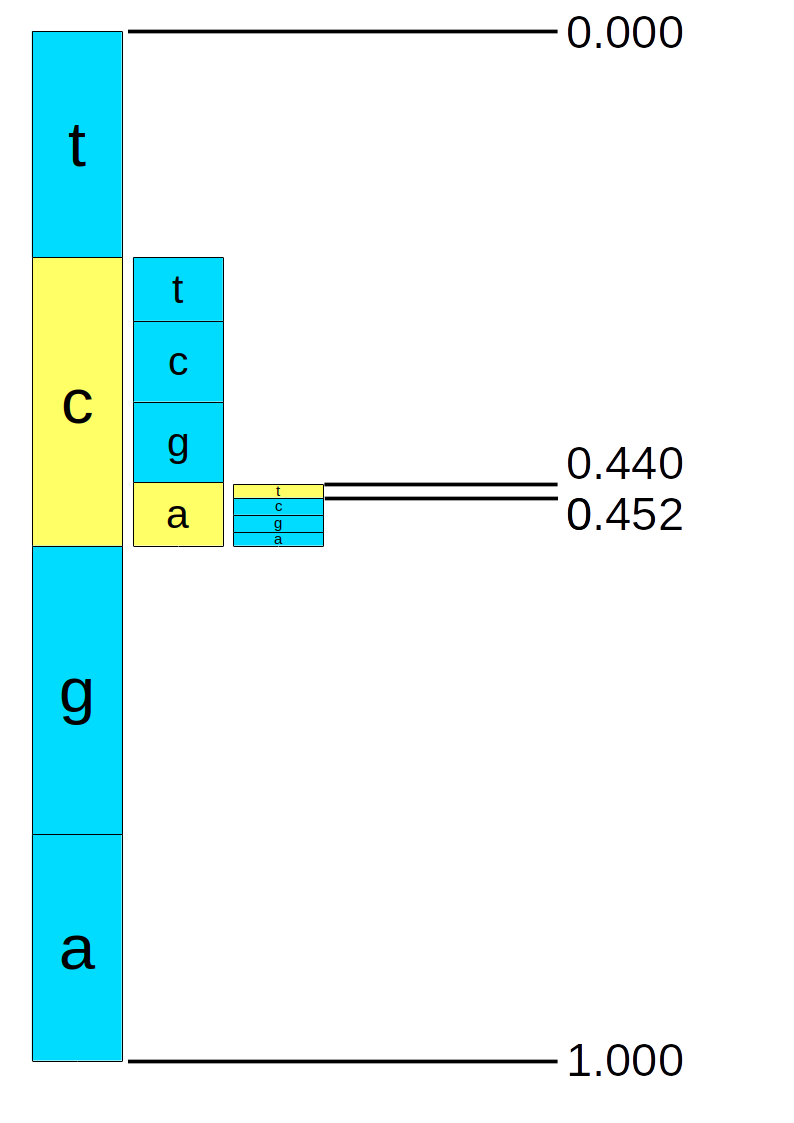
\includegraphics[height=250pt, keepaspectratio=true]{img/range_code.png}

Decoding is simply the reverse of this.  In the above picture we can see that 0.45 would read off `c', `a' and `t' by repeatedly comparing the symbol ranges to the current range and using those to identify the symbol and produce a new range.

\begin{threeparttable}[t]
\begin{tabular}{rrrr}
\hline
\textbf{Range low} & \textbf{Range high} & \textbf{Fraction into range} & \textbf{Symbol}\\
\hline
0.000 & 1.000 & 0.450 & c\\
0.200 & 0.500 & 0.833\tnote{\textbf{a}} & a\\
0.440\tnote{\textbf{b}} & 0.500 & 0.167 & t\\
\hline
\end{tabular}
\begin{tablenotes}
\item{\textbf{a.}} 0.45 into range 0.2 to 0.5: $(0.45-0.2)/(0.5-0.2) = 0.833$.
This falls within the 0.8 to 1.0 symbol range for `a'.
\item{\textbf{b.}} `a' symbol range 0.8 to 1.0 applied to range 0.2 to 0.5:  $0.2+0.8\times(0.5-0.2) = 0.44$ and $0.2+1.0\times(0.5-0.2) = 0.5$.
\end{tablenotes}
\end{threeparttable}

Note: The above example not how the actual implementation works\footnote{This implementation was designed by Eugene Shelwein, based on Michael Schindler's earlier work.}.
For efficiency, we use integer values having a starting range of 0 to $2^{32}-1$.
We write out the top 8-bits of the range when low and high become the same value.
Special care needs to be taken to handle small values are are numerically close but stradding a top byte value, such as 0x37ffba20 to 0x38000034.
The decoder does not need to do anything special here, but the encoder must track the number of 0xff or 0x00 values to emit in order to avoid needing arbitrary precision integers.

Pseudocode for the range codec decoding follows.
This implementation uses code (next few bytes in the current bit-stream) and range instead of low and high, both 32-bit unsigned integers.
This specification focuses on decoding, but given the additional complexity of the precision overflows in encoder we describe this implementation too.

\textsc{RangeDecodeCreate} initialises the range coder, reading the first bytes of the compressed data stream.

\begin{algorithmic}[1]
\Function{RangeDecodeCreate}{}
  \settowidth{\maxwidth}{range\ }
  %\State \algalign{low}{\gets} $0$\Comment{32-bit unsigned}
  \State \algalign{range}{\gets} $2^{32}-1$\Comment{Maximum 32-bit unsigned value}
  \State \algalign{code}{\gets} $0$\Comment{32-bit unsigned}
  \For{$i \gets 0$ to $4$}
    \State $code \gets (code \shiftl 8) + $\Call{ReadUint8}{}
  \EndFor
  \State $code \gets code \bitand 2^{32}-1$
  \State \Return this range coder ($range$, $code$)
\EndFunction
\end{algorithmic}

Decoding each symbol is in two parts; getting the current frequency and updating the range.

\begin{algorithmic}[1]
\Function{RangeGetFreq}{$tot\_freq$}
  \State $range \gets range \bdiv tot\_freq$
  \State \Return $code \bdiv range$
\EndFunction
\end{algorithmic}

\begin{algorithmic}[1]
\Procedure{RangeDecode}{$sym\_low, sym\_freq, tot\_freq$}
  \settowidth{\maxwidth}{range\ }
  \State \algalign{code}{\gets} $code - sym\_low \times range$
  \State \algalign{range}{\gets} $range \times sym\_freq$

  \While{$range < 2^{24}$} \Comment{Renormalise}
    \settowidth{\maxwidth}{range\ }
    \State \algalign{range}{\gets} $range \shiftl 8$
    \State \algalign{code}{\gets} $(code\shiftl8) + $\Call{ReadUint8}{}
  \EndWhile
\EndProcedure
\end{algorithmic}

As mentioned above, the encoder is more complex as it cannot shift out the top byte until it has determined the value.
This can take a considerable while if our current low / high (low + range) are very close but span a byte boundary, such as 0x37ffba20 to 0x38000034, where ultimately we will later emit either 0x37 or 0x38.
To handle this case, when the range gets too small but the top bytes still differ, the encoder caches the top byte of low (0x37) and keeps track of how many 0xff or 0x00 values will need to be written out once we finally observe which value the range has shrunk to.

The \textsc{RangeEncode} function is a straight forward reversal of the \textsc{RangeDecode}, with the exception of the special code for shifting the top byte out of the $low$ variable.

\begin{algorithmic}[1]
\Procedure{RangeEncode}{$sym\_low, sym\_freq, tot\_freq$}
  \settowidth{\maxwidth}{old\_low\ }
  \State \algalign{old\_low}{\gets} $low$
  \State \algalign{range}{\gets} $range \bdiv tot\_freq$
  \State \algalign{low}{\gets} $low + sym\_low \times range$
  \State \algalign{range}{\gets} $range \times sym\_freq$

  \Statex
  \If{low < old\_low}
    \State $carry \gets 1$ \Comment{overflow}
  \EndIf
  \While{$range < 2^{24}$} \Comment{Renormalise}
    \settowidth{\maxwidth}{range\ }
    \State \algalign{range}{\gets} $range \shiftl 8$
    \State \Call{RangeShiftLow}{}
  \EndWhile
\EndProcedure
\end{algorithmic}

\textsc{RangeShiftLow} is the main heart of the encoder renormalisation.
It tracks the total number of extra bytes to emit and $carry$ indicates whether they are a string of 0xFF or 0x00 values.

\begin{algorithmic}[1]
\Procedure{RangeShiftLow}{}
  \If{$low < $ 0xff000000 $\logor carry \ne 0$}
    \If{$carry = 0$}
      \State \Call{WriteByte}{$cache$} \Comment{top byte $cache$ plus FFs}
      \While{$FFnum > 0$}
        \State \Call{WriteByte}{0xff}
        \State $FFnum \gets FFnum - 1$
      \EndWhile
    \Else
      \State \Call{WriteByte}{$cache + 1$} \Comment{top byte $cache+1$ plus 00s}
      \While{$FFnum > 0$}
        \State \Call{WriteByte}{0}
        \State $FFnum \gets FFnum - 1$
      \EndWhile
    \EndIf
    \State $cache \gets low \shiftr 24$ \Comment{Copy of top byte ready for next flush}
    \State $carry \gets 0$
  \Else
    \State $FFnum \gets FFnum + 1$
  \EndIf
  \Statex
  \State $low \gets low \shiftl 8$
\EndProcedure
\end{algorithmic}

For completeness, the Encoder initialisation and finish functions are below.

\begin{algorithmic}[1]
\Procedure{RangeEncodeStart}{}
  \settowidth{\maxwidth}{FFnum\ }
  \State \algalign{low}{\gets} $0$
  \State \algalign{range}{\gets} $2^{32}-1$
  \State \algalign{FFnum}{\gets} $0$
  \State \algalign{carry}{\gets} $0$
  \State \algalign{cache}{\gets} $0$
\EndProcedure
\end{algorithmic}

\begin{algorithmic}[1]
\Procedure{RangeEncodeEnd}{}
  \For{$i \gets 0$ to $4$} \Comment{Flush any residual state in $low$}
    \State \Call{RangeShiftLow}{}
  \EndFor
\EndProcedure
\end{algorithmic}


\subsection{Statistical Modelling}

The probabilities passed to the range coder may be fixed for all scenarios (as we had in the ``cat'' example), or they may be adaptive and context aware.
For example the letter `u' occurs around 3\% of time in English text, but if the previous letter was `q' it is close to 100\% and if the previous letter was `u' it is close to 0\%.
Using the previous letter is known as an Order-1 entropy encoder, but the context can be anything.
We can also adaptively adjust our probabilities as we encode or
decode, learning the likelihoods and thus avoiding needing to store
frequency tables in the data stream covering all possible contexts.

To do this we use a statistical model, containing an array of symbols $S$ and their frequencies $F$.
The sum of these frequences must be less than $2^{16}-32$.
When they get too high, they are renormalised by approximately halving the frequencies (ensuring none drop to zero).

Typically an array of models are used where the array index represents the current context.

To encode any symbol the entropy encoder needs to know the frequency of the symbol to encode, the cumulative frequencies of all symbols prior to this symbol, and the total of all frequencies.
For decoding a cumulative frequency is obtained given the frequency total and the appropriate symbol is found matching this frequency.
Symbol frequencies are updated after each encode or decode call and the symbols are kept in order of most-frequent symbol first in order to  reduce the overhead of scanning through the cumulative frequencies.

\textsc{ModelCreate} initialises a model by setting every symbol to have a frequency of 1.
(At no point do we permit any symbol to have zero frequency.)

\begin{algorithmic}[1]
\Function{ModelCreate}{$num\_sym$}
  \State $total\_freq \gets num\_sym$
  \State $max\_sym \gets num\_sym-1$
  \For{$i \gets 0$ to $max\_sym$}
    \State $S_i \gets i$
    \State $F_i \gets 1$
  \EndFor
  \State \Return this model ($total\_freq$, $max\_sym$, $S$, $F$)
\EndFunction
\end{algorithmic}

\textsc{ModelDecode} is called once for each decoded symbol.
It returns the next symbol and updates the model frequencies automatically.

\begin{algorithmic}[1]
\Function{ModelDecode}{rc}
  \State $freq \gets$ $rc.$\Call{RangeGetFrequency}{$total\_freq$}
  \State $x \gets 0$
  \State $acc \gets 0$
  \While{$acc + F_x \le freq$}
    \State $acc \gets acc + F_x$
    \State $x \gets x+1$
  \EndWhile
  \State $rc.$\Call{RangeDecode}{$acc,\ F_x,\ total\_freq$}
  \State $F_x \gets F_x + 16$ \Comment{Update model frequencies}
  \State $total\_freq \gets total\_freq + 16$
  \If{$total\_freq > 2^{16}-17$}
    \State \Call{ModelRenormalise}{}
  \EndIf
  \State $sym \gets S_x$
  \If{$x > 0 \logand F_x > F_{x-1}$}
    \State \Call{Swap}{$F_x$, $F_{x-1}$}
    \State \Call{Swap}{$S_x$, $S_{x-1}$}
  \EndIf
  \State \Return $sym$
\EndFunction
\end{algorithmic}

\textsc{ModelRenormalise} is called whenever the total frequencies get too high.
The frequencies are halved, taking sure to avoid any zero frequencies being created.

\begin{algorithmic}[1]
\Procedure{ModelRenormalise}{}
  \State $total\_freq \gets 0$
  \For{$i \gets 0$ to $max\_sym$}
    \State $F_i \gets F_i - (F_i \bdiv 2)$
    \State $total\_freq \gets total\_freq + F_i$
  \EndFor
\EndProcedure
\end{algorithmic}

\subsection{Order-0 and Order-1 Encoding}

We can combine the model defined above and the range coder to provide a simple function to perform Order-0 entropy decoder.

\begin{algorithmic}[1]
\Function{DecodeOrder0}{$len$}
  \State $max\_sym \gets $\Call{ReadUint8}{}
  \If{$max\_sym = 0$}
    \State $max\_sym \gets 256$
  \EndIf
  \State $model\_lit \gets $\Call{ModelCreate}{$max\_sym$}
  \Statex
  \State $rc \gets $\Call{RangeDecodeCreate}{}
  \For{$i \gets 0$ to $len-1$}
    \State $out_i \gets model\_lit.$\Call{ModelDecode}{$rc$}
  \EndFor
  \State \Return $out$
\EndFunction
\end{algorithmic}

The Order-1 variant simply uses an array of models and selects the appropriate model based on the previous value encoded or decoded.
This array index is our ``context''.

\begin{algorithmic}[1]
\Function{DecodeOrder1}{$len$}
  \State $max\_sym \gets $\Call{ReadUint8}{}
  \If{$max\_sym = 0$}
    \State $max\_sym \gets 256$
  \EndIf
  \For{$i \gets 0$ to $max\_sym-1$}
    \State $model\_lit_i \gets $\Call{ModelCreate}{$max\_sym$}
  \EndFor
  \Statex
  \State $rc \gets $\Call{RangeDecodeCreate}{}
  \State $last \gets 0$
  \For{$i \gets 0$ to $len-1$}
    \State $out_i \gets model\_lit_{last}.$\Call{ModelDecode}{$rc$}
    \State $last \gets out_i$
  \EndFor
  \State \Return $out$
\EndFunction
\end{algorithmic}

\subsection{RLE with Order-0 and Order-1 Encoding}

The \textsc{DecodeOrder0} and \textsc{DecodeOrder1} codecs can be expanded to include a count of how many runs of each symbol should be decoded.
Both order 0 and order 1 variants are possible.

After the symbol is decoded, the run length must be decoded to
indicate how many \emph{extra} copies of this symbol occur.  Long runs
are broken into a series of lengths of no more than 3.  If length 3
is decoded it indicates we must decode an additional length and add to
the current one.  The context used for the run length model is the
symbol itself for the initial run, 256 for the first continuation run
(if $\ge 4$) and 257 for any further continuation runs.  Thus encoding
10 `A' characters would first store symbol `A' followed by run length
3 (with context `A'), length 3 (context 256), length 3 (context
257), and length 1 (context 258).

For example, if we have the string ``RRRRUNN'' we will decode
symbol `R' run 3, symbol `U' run 0, symbol `N' run 1.

\begin{algorithmic}[1]
\Function{DecodeRLE0}{$len$}
  \State $max\_sym \gets $\Call{ReadUint8}{}
  \If{$max\_sym = 0$}
    \State $max\_sym \gets 256$
  \EndIf
  \State $model\_lit \gets $\Call{ModelCreate}{$max\_sym$}

  \For{$i \gets 0$ to $257$}
    \State $model\_run_i \gets $\Call{ModelCreate}{$4$}
  \EndFor
  \Statex
  \State $rc \gets $\Call{RangeDecodeCreate}{}
  \State $i \gets 0$
  \While{$i < len$}
    \State $out_i \gets model\_lit.$\Call{ModelDecode}{$rc$}
    \State $part \gets model\_run_{out_i}.$\Call{ModelDecode}{$rc$}
    \State $run \gets part$
    \State $rctx \gets 256$
    \While{$part = 3$}
      \State $part \gets model\_run_{rctx}.$\Call{ModelDecode}{$rc$}
      \State $rctx \gets 257$
      \State $run \gets run + part$
    \EndWhile
    \For{$j \gets 1$ to $run$}
      \State $out_{i+j} \gets out_i$
    \EndFor
    \State $i \gets run+1$
  \EndWhile
  \State \Return $out$
\EndFunction
\end{algorithmic}

The order-1 run length variant is identical to order-0 except the
previous symbol is used as the context for the next literal.  The
context for the run length does not change.

\begin{algorithmic}[1]
\Function{DecodeRLE1}{$len$}
  \State $max\_sym \gets $\Call{ReadUint8}{}
  \If{$max\_sym = 0$}
    \State $max\_sym \gets 256$
  \EndIf
  \For{$i \gets 0$ to $max\_sym-1$}
    \State $model\_lit_i \gets $\Call{ModelCreate}{$max\_sym$}
  \EndFor
  \For{$i \gets 0$ to $257$}
    \State $model\_run_i \gets $\Call{ModelCreate}{$4$}
  \EndFor
  \Statex
  \State $rc \gets $\Call{RangeDecodeCreate}{}
  \State $last \gets 0$
  \State $i \gets 0$
  \While{$i < len$}
    \State $out_i \gets model\_lit_{last}.$\Call{ModelDecode}{$rc$}
    \State $last \gets out_i$
    \State $part \gets model\_run_{last}.$\Call{ModelDecode}{$rc$}
    \State $run \gets part$
    \State $rctx \gets 256$
    \While{$part = 3$}
      \State $part \gets model\_run_{rctx}.$\Call{ModelDecode}{$rc$}
      \State $rctx \gets 257$
      \State $run \gets run + part$
    \EndWhile
    \For{$j \gets 1$ to $run$}
      \State $out_{i+j} \gets last$
    \EndFor
    \State $i \gets run+1$
  \EndWhile
  \State \Return $out$
\EndFunction
\end{algorithmic}

%\subsection{General Purpose Entropy Encoder}

We wrap up the Order-0 and 1 entropy encoder, both with and without run length encoding, into a data stream that specifies the type of encoded data and also permits a number of additional transformations to be applied.
These transformations support bit packing (for example a data block with only 4 distinct values can be packed with 4 values per byte), no-op for tiny data blocks where entropy encoding would grow the data and N-way interleaving of the 8-bit components of a 32-bit value.

\begin{table}[h]
\centering
\begin{tabular}{|r|r|r|r|p{9cm}|l|}
\hline
\multicolumn{2}{|r|}{\textbf{Bits} } & \textbf{Type}  & \textbf{Name} & \multicolumn{2}{p{9cm}|}{\textbf{Description}} \\
\hline
\multicolumn{2}{|r|}{8} & uint8 & $flag$ & \multicolumn{2}{p{9cm}|}{Data format bit field}\\
\cline{1-6}

\multicolumn{6}{|l|}{}\\[-0.3em]
\multicolumn{6}{|l|}{\textit{Unless \textsc{NoSize} flag is set:} } \\
\cline{2-5}
& ? & uint7 & ulen & Uncompressed length & \\
\cline{2-5}

\multicolumn{6}{|l|}{}\\[-0.3em]
\multicolumn{6}{|l|}{\textit{If \textsc{Stripe} flag is set:} } \\
\cline{2-5}
& ? & uint8 & N & Number of sub-streams & \\
& ? & uint7[] & clen[] & N copies of compressed sub-block length & \\
& ? & uint8[] & cdata[] & N copies of Compressed data sub-block (recurse) & \\
\cline{2-5}

\multicolumn{6}{|l|}{}\\[-0.7em]
\multicolumn{6}{|l|}{\textit{If \textsc{Cat} flag is set (and \textsc{Stripe} flag is unset):} } \\
\cline{2-5}
& ? & uint8[] & udata & Uncompressed data stream & \\
\cline{2-5}

\multicolumn{6}{|l|}{}\\[-0.7em]
\multicolumn{6}{|l|}{\textit{If \textsc{Pack} flag is set (and neither \textsc{Stripe} or \textsc{Cat} flags are set):} } \\
\cline{2-5}
& ? & uint8[] & pack\_meta & Pack lookup table & \\
\cline{2-5}

\multicolumn{6}{|l|}{}\\[-0.7em]
\multicolumn{6}{|l|}{\textit{If neither \textsc{Stripe} or \textsc{Cat} flags are set:} } \\
\cline{2-5}
& ? & uint8[] & cdata & Entropy encoded data stream (see \textsc{Order} / \textsc{RLE} / \textsc{Ext} flags) & \\
\cline{2-5}
\multicolumn{6}{|l|}{}\\
\hline
\end{tabular}
\end{table}

The first byte of our generalised data stream is a bit-flag detailing the type of transformations and entropy encoders to be combined, followed by optional meta-data, followed by the actual compressed data stream.
The bit-flags are defined below, but note not all combinations are permitted.

\begin{threeparttable}[t]
\begin{tabular}{llll}
\hline
\textbf{Bit AND value} & \textbf{Code} & \textbf{Description} \\
\hline
1 & \textsc{Order}\tnote{\textbf{a}} & Order-0 or Order-1 entropy coding. \\
2 & reserved & Reserved (for possible order-2/3)\\
4 & \textsc{Ext} & ``External'' compression via bzip2\\
8 & \textsc{Stripe}\tnote{\textbf{b}} & N-way interleaving of byte streams.\\
16 & \textsc{NoSize} & original size is not recorded (used by \textsc{Stripe})\\
32 & \textsc{Cat}\tnote{\textbf{b}} & Data is uncompressed\\
64 & \textsc{RLE}\tnote{\textbf{a}} & Run length encoding, with runs and literals encoded separately\\
128 & \textsc{Pack} & Pack 2, 4, 8 or infinite symbols per byte.\\
\hline
\end{tabular}
\begin{tablenotes}
\item{\textbf{a.}} Has no effect when \textsc{Ext} flag is set.
\item{\textbf{b.}} Not to be used in conjunction with other flags
  except \textsc{Pack} and \textsc{NoSize}.
\end{tablenotes}
\end{threeparttable}

Of these \textsc{Stripe} is the most complex.
As with the rANS4x16 encoder, the data is rearranged such that every
$N^{th}$ byte is adjacent in a single block producing N distinct sub-blocks.
Each of the N streams is then itself compressed using this compression format.

For example an input block of small unsigned 32-bit little-endian numbers may use RLE for the first three streams as they are mostly zero, and a non-RLE Order-0 entropy encoder of the last stream.
Normally our data format will include the decoded size, but with \textsc{Stripe} we can omit this from the internal compressed streams as we know their size will be a computable fraction of the combined data.

The data layout differs for each of these bit types, as described below in the \textsc{ArithDecode} function.
Some of these can be used in combination, so the order needs to be observed.
The Pack format has additional meta data.
This is decoded first, before entropy decoding and finally expanding thespecified pack transformation after decompression.
For example value 193 is indicates a byte stream should be decoded with an RLE aware order-1 entropy encoder and then unpacked.

\begin{algorithmic}[1]
\Function{ArithDecode}{$len$}
  \State $flags \gets $\Call{ReadUint8}{}
  \If{$flags \bitand$ \textsc{NoSize} $\ne 0$}
    \State $len \gets$\Call{ReadUint7}{}
  \EndIf
  \If{$flags \bitand$ \textsc{Stripe}}
    \State $data \gets $\Call{DecodeSTRIPE}{$len$}
    \State \Return $data$
  \EndIf{}
  \If{$flags \bitand$ \textsc{Pack}}
    \State $pack\_len \gets len$
    \State $(P,\ nsym,\ len) \gets $\Call{DecodePackMeta}{}
  \EndIf
  \Statex \Comment{Entropy Decoding}
  \If{$flags \bitand$ \textsc{Cat}}
    \State $data \gets $\Call{ReadData}{$len$}
  \ElsIf{$flags \bitand$ \textsc{Ext}}
    \State $data \gets $\Call{DecodeEXT}{$len$}
  \ElsIf{$flags \bitand$ \textsc{RLE}}
    \If{$flags \bitand$ \textsc{Order}}
      \State $data \gets $\Call{DecodeRLE1}{$len$}
    \Else
      \State $data \gets $\Call{DecodeRLE0}{$len$}
    \EndIf
  \Else
    \If{$flags \bitand$ \textsc{Order}}
      \State $data \gets $\Call{DecodeOrder1}{$len$}
    \Else
      \State $data \gets $\Call{DecodeOrder0}{$len$}
    \EndIf
  \EndIf
  \Statex \Comment{Apply data transformations}
  \If{$flags \bitand$ \textsc{Pack}}
    \State $data \gets $\Call{DecodePack}{$data$, $P$, $nsym$, $pack\_len$}
  \EndIf
  \State \Return $data$
  \EndFunction
\end{algorithmic}

The specifics of each sub-format are described below, in the order (minus meta-data specific shuffling) they are applied.

\begin{itemize}
\item{\textbf{\textsc{Stripe}}:}
The byte stream consists of a 7-bit encoded uncompressed length and a
byte holding the number of substreams $N$, and their 7-bit encoded
compressed data streams lengths.  This is then followed by the
substreams themselves, each of which is a valid $cdata$ stream as
defined above, hence this offers a recursive mechanism as each
substream has its own format byte.

The total uncompressed byte stream is then an interleaving of one byte
in turn from each of the N substreams (in order of 1st to Nth).  Thus
an array of 32-bit unsigned integers could be unpacked using
\textsc{Stripe} to compress each of the 4 8-bit components together with
their own algorithm.

\begin{algorithmic}[1]
\Function{RansDecodeStripe}{$len$}
  \State $N \gets $\Call{ReadUint8}{}
  \For{$j \gets 0$ to $N$} \Comment{Fetch N compressed lengths}
    \State $clen_j \gets $\Call{ReadUint7}{}
  \EndFor
  \Statex
  \For{$j \gets 0$ to $N$} \Comment{Decode N streams}
    \State $ulen_j \gets (len \bdiv N) + ((len \bmod N) > j)$
\Comment{$(x > y)$ expression being 1 if true, 0 if false}
    \State $T_j \gets $\Call{ArithDecode}{$ulen_j$}
  \EndFor
  \Statex
%  \For{$i \gets 0$ to $len - 1$} \Comment{Interleave}
%    \State $out_i \gets T_{(i \bmod N),\ (i \bdiv N)}$
%  \EndFor
  \For{$j \gets 0$ to $N - 1$} \Comment{Interleave}
    \For{$i \gets 0$ to $ulen_j - 1$}
      \State $out_{i \times N + j} \gets T_{j,i}$
    \EndFor
  \EndFor
  \State \Return $out$
\EndFunction
\end{algorithmic}

\item{\textbf{\textsc{NoSize}}:}
Do not store the size of the uncompressed data stream.
This information is not required when the data stream is one of the four sub-streams in the \textsc{Stripe} format.

\item{\textbf{\textsc{Cat}}:}
If present, all other bit flags should be nul, with the possible
exception of \textsc{NoSize} or \textsc{Pack}.

The uncompressed data stream is the same as the compressed stream.
This is useful for very short data where the overheads of compressing are too high.

\item{\textbf{\textsc{Order}}:}
Bit field defining order-0 (unset) or order-1 (set) entropy encoding, as described above by the \textsc{DecodeOrder0} and \textsc{DecodeOrder1} functions.

\item{\textbf{\textsc{RLE}}:}
Bit field defining whether the Order-0 and Order-1 encoding should also use a run-length.
When set, the \textsc{DecodeRLE0} and \textsc{DecodeRLE1} functions will be used instead of \textsc{DecodeOrder0} and \textsc{DecodeOrder1}.

\item{\textbf{\textsc{Ext}}:}
Instead of using the adaptive arithmetic coder for decompression (with or without RLE), this uses an compression codec defined in an ``external'' library.
Currently the only supported such codec is Bzip2.
In future more may be added, so the magic number \emph{must} be validated to check the codec being used.

Given bzip2 is already supported elsewhere in CRAM, the purpose of adding it here is to permit bzip2 compression after \textsc{Pack} and \textsc{Stripe} transformations.
This may be tidied up in later CRAM releases to clarify the separation between compression codecs and data transforms, but that requires more major restructuring so for compatibility with v3.0 these have been placed into this single codec.

\begin{algorithmic}[1]
\Function{DecodeExt}{$len$}
  \If{Bzip2 magic number is present}
    \State \Return \Call{DecodeBzip2}{$len$}
  \Else
    \State Error
  \EndIf
\EndFunction
\end{algorithmic}

\item{\textbf{\textsc{Pack}}:}
Data containing only 1, 2, 4 or 16 distinct values can have multiple
values packed into a single byte (infinite, 8, 4 or 2).  The distinct
symbol values do not need to be adjacent as a mapping table $P$
converts mapped value $x$ to original symbol $P_x$.

The packed format is split into uncompressed meta-data (below) and the
compressed packed data as described in the rANS 4x16 bit-packing section.
The same \textsc{DecodePackMeta} and \textsc{DecodePack} functions are used.

\end{itemize}

\section{Name tokenisation codec}

Sequence names (identifiers) typically follow a structured pattern and compression based on columns within those structures usually leads to smaller sizes.
The sequence name (identifier) tokenisation relies heavily on the General Purpose Entropy Encoder described above.

As an example, take a series of names:

\begin{verbatim}
I17_08765:2:123:61541:01763#9
I17_08765:2:123:1636:08611#9
I17_08765:2:124:45613:16161#9
\end{verbatim}

We may wish to tokenise each of these into 7 tokens, e.g.
``I17\_08765:2:'', ``123'', ``:'', ``61541'', ``:'', ``01763''and
``\#9''. Some of these are multi-byte strings, some single characters,
and some numeric, possibily with a leading zero.  We also observe some
regularly have values that match the previous line (the initial prefix
string, colons, ``\#9'') while others are numerically very close to the
value in the previous line (124 vs 123).

The name tokeniser compares each name against a previous name (which
is not necessarily the one immediately prior) and encodes this name
either as a series of differences to the previous name or marking it
as an exact duplicate.  A maximum of 128 tokens are permitted within
any single read name.

Token IDs (types) are listed below.

\begin{tabular}{lllp{10cm}}
\hline
\textbf{ID} & \textbf{Type} & \textbf{Value} & \textbf{Description}\\
\hline
 0 & TYPE    & Type    & Used to determine the type of token at a given position. \\
\hline
 5 & DUP     & Integer (distance) & The entire name is a duplicate of an earlier one.  Used in position 0 only.\\
 6 & DIFF    & Integer (distance) & The entire name is differs to earlier ones.  Used in position 0 only.\\
\hline
 1 & STRING  & String  & A nul-terminated string of characters \\
 2 & CHAR    & Byte    & A single character \\
 7 & DIGITS  & $0 \le$ Int $< 2^{32}$ & A numerical value, not containing a leadng zero \\
 3 & DIGITS0 & $0 \le$ Int $< 2^{32}$ & A numerical value possibly starting in leading zeros \\
 4 & DZLEN   & Int length & Length of associated DIGITS0 token.\\
 8 & DELTA  & $0 \le$ Int $< 256$   & A numeric value being stored as the difference to the numeric value of this token on the previous name. \\
 9 & DELTA0 & $0 \le$ Int $< 256$ & As DELTA, but for numeric values starting with leading zeros \\
10 & MATCH   & (none) & This token is identical type and value to the same position in the previous name (NB: not permitted for DELTA/DELTA0)\\
11 & NOP & (none) & Does nothing\\
12 & END     & (none) & Marks end of name\\
\hline
\end{tabular}

The tokens and values are stored in a 2D array of byte streams,
$B_{pos,type}$, where pos 0 is reserved for name meta-data (whether it
is a duplicate name) and pos 1 onwards is for the first, second and
later tokens.  $Type$ is one of the token types listed above,
corresponding to the type of data being stored.  Some token types may
also have associated values.  $B_{pos,\texttt{TYPE}}$ ($type$) holds the token
type itself and that is then used to retrieve any associated
value(s) if appropriate from $B_{pos,type}$.  Thus multiple types at the same token
position will have their values encoded in distinct data streams,
e.g. if position 5 is of type either DIGITS or DELTA then data streams
will exist for $B_{5,\texttt{TYPE}}$, $B_{5,\texttt{DIGITS}}$ and $B_{5, \texttt{DELTA}}$.
Decoding per name continues until a token of type END is observed.

More detail on the token types is given below.

\begin{itemize}
\item{\textbf{TYPE}:}
This is the first token fetched at each token position.  It holds the
type of the token at this position, which in turn may then require
retrieval from type-specific data streams at this position.

For position 0, the TYPE field indicates whether this record is an
exact duplicate of a prior read name or has been encoded as a delta to
an earlier one.

\item{\textbf{DUP}, \textbf{DIFF}:}
These types are fetched for position 0, at the start of each new
identifier.  The value is an integer value describing how many reads
before this (with 1 being the immediately previous name) we are
comparing against.  When we refer to ``previous name'' below, we
always mean the one indicated by the DIFF field and not the one
immediately prior to the current name.

The first record will have a DIFF of zero and no delta or match
operations are permitted.

\item{\textbf{STRING}:}
We fetch one byte at a time from the value byte stream, appending to the
name buffer until the byte retrieved is zero.  The zero byte is not
stored in the name buffer.
For purposes of token type MATCH, a match is defined as entirely
matching the string including its length.

\item{\textbf{CHAR}:}
Fetch one single byte from the value byte stream and append to the name buffer.

\item{\textbf{DIGITS}:}
Fetch 4 bytes from the value byte stream and intrepret these as a little
endian unsigned integer.  This is appended to the name buffer as
string of base-10 digits, most significant digit first.  Larger
values may be represented, but will require multiple DIGITS tokens.
Negative values may be encoded by treating the minus sign as a CHAR or
STRING and storing the absolute value.

\item{\textbf{DIGITS0}, \textbf{DZLEN}:}
This fetches the 4 byte value from $B_{pos,DIGITS0}$ and a 1 byte
length from $B_{pos,DZLEN}$.  As per DIGITS, the value is intrepreted as a
little endian unsigned integer.  The length indicates the total
size of the numeric value when displayed in base 10 which must be
greater than $\log_{10}(value)$ with any remaining length indicating
the number of leading zeros.  For example if DIGITS0 value is 123 and
DZLEN length is 5 the string ``00123'' must be appended to the name.

For purposes of the MATCH type, both value and length must match.

\item{\textbf{DELTA}:}
Fetch a 1 byte value and add this to the DIGITS value from the
previous name.
The token in the prior name must be of type DIGITS or DELTA.

MATCH is not supported for this type.

\item{\textbf{DELTA0}:}
As per DELTA, but the 1 byte value retrieved is added to the DIGITS0
value in the previous name.  No DZLEN value is retrieved, with the
length from the previous name being used instead.
The token in the prior name must be of type DIGITS0 or DELTA0.

MATCH is not supported for this type.

\item{\textbf{MATCH}:}
This token matches the token at the same position in the previous
name.  (The previous name is permitted to also have a MATCH token at
this position, in which case it recurses to its previous name.)

MATCH is only valid when the token being matched against is CHAR,
STRING, DIGITS, DIGITS0 or MATCH.  (I.e. matching a numeric delta will not
repeat the delta increment.)

No value is needed for MATCH tokens.

\item{\textbf{NOP}:}
This token type does nothing.
The purpose of this is simply to permit skipping tokens in order to
keep token numbers in sync, such as when processing ``10'' vs ``-10''
with the latter needing an additional ``-'' token.

\item{\textbf{END}:}
Marks the end of the name.  A nul byte is added to the name output
buffer.  No value is needed for END tokens.
\end{itemize}

Decoding needs some simple functions to read successive bytes from our token byte streams, as 8-bit characters or unsigned integers, as 32-bit unsigned integers and nul-terminated strings.  We reuse the \textsc{ReadUint32} and related functions with the byte array specified as input.

\begin{algorithmic}[1]
\Statex
\Statex \textit{(Convert an integer to a string form in base-10 digits, at least $len$ bytes long with leading zeros)}
\Function{LeftPadNumber}{$val,\ len$}
  \State $str \gets val$ \Comment{Implicit language-specific Integer to String conversion}
  \While{\Call{Length}{$str$} < $len$}
    \State $str \gets$ `$0$' $ \concat str$
  \EndWhile
  \State \Return $str$
\EndFunction
\end{algorithmic}

For the main name decoding loop, we use a single dimensional array of
names decoded so far, $N$, and a two dimensional array of their tokens
$T$ (indexed by name number $n$ and token position $t$ within that
name).  We define a function to decode the $n^{th}$ name ($N_n$) using
a previous $m^{th}$ name ($N_m$).  The tokens $T$ are used in
\texttt{MATCH} and \texttt{DELTA} token types to copy data from when
constructing the name.

Now we have the basic primitives for pulling from the $B$ byte
streams, decoding the $n^{th}$ individual name is as
follows\footnote{For simplicity of algorithm description, we take a
  flexible approach as to whether we read/write $T$ in numeric or
  string form.  For example a \texttt{DELTA} token will fetch the
  previous token as a string, interpret it as a numeric value, add to
  it, and then write it back as a string.  Practical implementations
  may wish to separate out T into distinct integer and string
  arrays.}:


\begin{algorithmic}[1]
\Statex
\Statex \textit{(Decodes the $n^{th}$ name, returning $N_n$ and updating globals $N_n$ and $T_n$)}
\Function{DecodeSingleName}{$n$}
  \State $type \gets$ \Call{ReadUint8}{$B_{0,\textit{TYPE}}$}
  \State $dist \gets$ \Call{ReadUint32}{$B_{0,type}$}
  \State $m \gets n-dist$
  \If{$type = $ \texttt{DUP}}
    \State $N_n \gets N_m$
    \State $T_n \gets T_m$ \Comment{Copy for all $T_{n,*}$}
    \State \Return $N_n$
  \EndIf
  \Statex
  \State $t \gets 1$ \Comment{Token number $t$}
  \Repeat
    \State $type \gets$ \Call{ReadUint8}{$B_{t,\texttt{TYPE}}$}
    \If{$type = $ \texttt{CHAR}}
      \State $T_{n,t} \gets$ \Call{ReadChar}{$B_{t,\texttt{CHAR}}$}
    \ElsIf{$type = $ \texttt{STRING}}
      \State $T_{n,t} \gets$ \Call{ReadString}{$B_{t,\texttt{STRING}}$}
    \ElsIf{$type = $ \texttt{DIGITS}}
      \State $T_{n,t} \gets$ \Call{ReadUint32}{$B_{t,\texttt{DIGITS}}$}
    \ElsIf{$type = $ \texttt{DIGITS0}}
      \State $d \gets$ \Call{ReadUnt32}{$B_{t,\texttt{DIGITS0}}$}
      \State $l \gets$ \Call{ReadUint8}{$B_{t,\texttt{DZLEN}}$}
      \State $T_{n,t} \gets$ \Call{LeftPadNumber}{$d,\ l$}
    \ElsIf{$type = $ \texttt{DELTA}}
      \State $T_{n,t} \gets T_{m,t} + $ \Call{ReadUint8}{$B_{t,\texttt{DELTA}}$}
    \ElsIf{$type = $ \texttt{DELTA0}}
      \State $d \gets T_{m,t} + $ \Call{ReadUint8}{$B_{t,\texttt{DELTA0}}$}
      \State $l \gets$ \Call{Length}{$T_{m,t}$} \Comment{String length including leading zeros}
      \State $T_{n,t} \gets$ \Call{LeftPadNumber}{$d,\ l$}
    \ElsIf{$type = $ \texttt{MATCH}}
      \State $T_{n,t} \gets T_{m,t}$
    \Else
      \State $T_{n,t} \gets$\ `'
    \EndIf
    \State $N_n \gets N_n \concat T_{n,t}$
    \State $t \gets t+1$
  \Until{$type = $ \texttt{END}}
  \State \Return $N_n$
\EndFunction
\end{algorithmic}

Given a complex name with both position and type specific values, this
can lead to many separate data streams.  The name tokeniser codec is
a format within a format, as the multiple byte streams $B_{pos,type}$
are serialised into a single byte stream.

The serialised data stream starts with two unsigned little endiand 32-bit
integers holding the total size of uncompressed name buffer and the
number of read names.  This is followed the array elements
themselves.

Token types, $ttype$ holds one of the token ID values listed above
in the list above, plus special values to indicate certain additional
flags.  Bit 6 (64) set indicates that this entire token data stream is a
duplicate of one earlier.  Bit 7 (128) set indicates the token
is the first token at a new position.  This way we only need to store
token types and not token positions.

The total size of the serialised stream needs to be already known, in
order to determine when the token types finish.

\begin{tabular}{|r|r|r|l|l|p{10cm}|}
\hline
\multicolumn{3}{|r|}{\textbf{Bytes}} & \textbf{Type} & \textbf{Name} & \textbf{Description}\\
\hline
\multicolumn{3}{|r|}{4} & uint32 & $uncomp\_length$ & Length of uncompressed name buffer\\
\multicolumn{3}{|r|}{4} & uint32 & $num\_reads$ & Number of read names\\
\multicolumn{3}{|r|}{1} & uint8  & $use\_arith$ & Whether compression is arithmetic (1) or rANS4x16 (0)\\
\hline
\multicolumn{6}{|l|}{\quad\textit{For each token data stream}}\\
\cline{2-6}
& \multicolumn{2}{r|}{1} & uint8 & $ttype$ & Token type code plus flags (64=duplicate, 128=next token position).\\
\cline{2-6}
& \multicolumn{5}{l|}{\textit{If ttype AND 64 (duplicate)}}\\
\cline{3-6}
& & 1 & uint8 & $dup\_pos$  & Duplicate from this token position\\
& & 1 & uint8 & $dup\_type$ & Duplicate from this token type ID\\
\cline{3-6}
& \multicolumn{5}{l|}{\textit{else if not duplicate}}\\
\cline{3-6}
& & ? & i7 & $clen$ & compressed length (7-bit encoding)\\
& & $clen$ & $cdata$ & stream & compressed data stream\\
\hline
\end{tabular}

A few tricks are used to remove some byte streams.  In addition to the explicit marking of duplicate bytes streams, if a byte stream of token types is entirely MATCH apart from the very first value it is discarded.  It is possible to regenerate this during decode by observing the other byte streams.  For example if we have a byte stream $B_{5,DIGITS}$ but no $B_{5,TYPE}$ then we assume the contents of $B_{5,TYPE}$ consist of one DIGITS type followed by as many MATCH types as are needed.

The $cdata$ stream itself is as described in the General Purpose Entropy Encoder section above, with the \textsc{ArithDecode} function.

\begin{algorithmic}[1]
\Statex
\Statex \textit{(Decodes and uncompressed the serialised token byte streams)}
\Function{DecodeTokenByteStreams}{$use\_arith$}
  \State $sz \gets 0$
  \State $t \gets -1$
  \Repeat
    \State $ttype \gets$ \Call{ReadUint8}{}
    \State $tok\_new \gets ttype \bitand 128$
    \State $tok\_dup \gets ttype \bitand 64$
    \State $type \gets ttype \bitand 63$
    \If{$tok\_new \ne 0$}
      \State $t \gets t+1$
      \If{$type \ne \texttt{TYPE}$}
        \State $B_{t,\texttt{TYPE}} \gets (type, \texttt{TOK\_MATCH}, \texttt{TOK\_MATCH}, ...)$\Comment{for $nnames-1$ times}
      \EndIf
    \EndIf
    \Statex
    \If{$tok\_dup \ne 0$}
       \State $dup\_pos \gets$ \Call{ReadUint8}{}
       \State $dup\_type \gets$ \Call{ReadUint8}{}
       \State $B_{t,type} \gets B_{dup\_pos,dup\_type}$
    \Else
      \State $clen \gets$ \Call{ReadUint7}{}
      \State $data \gets$ \Call{ReadData}{$clen$}
      \If{$use\_arith$}
        \State $B_{t,type} \gets$ \Call{ArithDecode}{}
      \Else
        \State $B_{t,type} \gets$ \Call{RansDecode4x16}{}
      \EndIf
    \EndIf
  \Until{\Call{EOF}{}}
  \State \Return $B$
\EndFunction
\end{algorithmic}

\begin{algorithmic}[1]
\Statex
\Statex \textit{(Decodes the $n^{th}$ name, returning $N_n$ and updating $N_n$ and $T_n$)}
\Function{DecodeNames}{}
  \State $ulen \gets$ \Call{ReadUint32}{}
  \State $nnames \gets$ \Call{ReadUint32}{}
  \State $use\_arith \gets$ \Call{ReadUint8}{}
  \State $B \gets$ \Call{DecodeTokenByteStreams}{$use\_arith$}

  \For{$n \gets 0$ to $nnames-1$}
    \State $N_n \gets$ \Call{DecodeSingleName}{$n$}
  \EndFor
  \State \Return $N$
\EndFunction
\end{algorithmic}


\section{FQZComp quality codec}

% Ideas to explore and TODO list:
%
% 1. Move param do_rev to global part.  It's all or nothing
%
% 2. Delta updates immediately on base 0 to base 1.  Maybe delay
%    initialisation so prevq is 1st base qual.
%
% 3. ReadArray pseudocode needs fixing.
%
% 4. Add param sel_offset to subtract from decoded sel.
%    Eg if we have 2 params and max_sel 3 (0..3) then we may want
%    sel 0/1 for 1st param and sel 0/1 (sel_offset 2) for 2nd?
%
% 5. Add len_bytes to param so we don't need Model_len[4] always.
%
% 6. Permit do_term and term_sym to put in newlines (or whatever)
%    after each record. (See 7 below for example)
%
% 7. Add dmap to apply to quals before doing the prevq != q check.
%    Reason is maybe we're not compressing qualities!  Eg SA:Z: tag
%    may be best using dmap , = 1 and everything else = 0.  Then
%    ``chr4,100,5,blah''; becomes delta 000012223456666.  dtab to
%    divide by 2 then allows it to track token number.
%    Each semi-colon separated text is a new record (qlen) and they're
%    joined together with term_sym (6. above).
%
% 8. Consider adding selector as context for model len, rev and dup.
%    This is important on mixed data sets.  Do we want full sel, or
%    quantised stab[sel]?

The FQZComp quality codec uses an adaptive statistical model to
predict the next quality value in a given context (comprised of
previous quality values, position along this sequence, whether the
sequence is the second in a pair, and a running total of number of
times the quality has changed in this sequence).

For each quality value, the models produce probabilities for all
possible next quality values, which are passed into an arithmetic
entropy encoder to encode or decode the actual next quality value.
The models are then updated based on the actual next quality in order
to learn the statistical properties of the quality data stream.  This
step wise update process is identical for both encoding and decoding.

The algorithm is a generalisation on the original fqzcomp program,
described in \textit{Compression of FASTQ and SAM Format Sequencing
  Data} by Bonfield JK, Mahoney MV (2013). PLoS ONE 8(3):
e59190. \url{https://doi.org/10.1371/journal.pone.0059190}

\subsection{FQZComp Models}

The FQZComp process utilises knowledge of the read lengths, complement
(qualities reversed) status, and a generic parameter selector, but in
order to maintain a strict separation between CRAM data series this
knowledge is stored (duplicated) within the quality data stream
itself.  Note the complement model is only needed in CRAM 3.1 as CRAM
4 natively stores the quality in the original orientation already.
Both reversed and duplication models have no context and are boolean
values.

The parameter selector model also has no context associated with it
and encodes $max\_sel$ distrinct values.  The selector value may be
quantised further using $stab$ to reduce the selector to fewer
sets of parameters.  This is useful if we wish to use the selector
bits directly in the context using the same parameters.  The selector
is arbitrary and may be used for distinguishing READ1 from READ2, as
a precalculated ``delta'' instead of the running total, distinguishing
perfect alignments from imperfect ones, or any other factor that is
shown to improve quality predictability and increase compression
ratio (average quality, number of mismatches, tile, swathe, proximity
to tile edge, etc).

The quality model has a 16-bit context used to address an array of
$2^{16}$ models, each model permitting $max\_sym$ distinct quality
values.  The context used is defined by the FQZcomp parameters, of
which there may be multiple sets, selected using the selector model.
There are 4 read length models each having $max\_sym$ of 256.  Each
model is used for the 4 successive bytes in a 32-bit length value.

\begin{center}
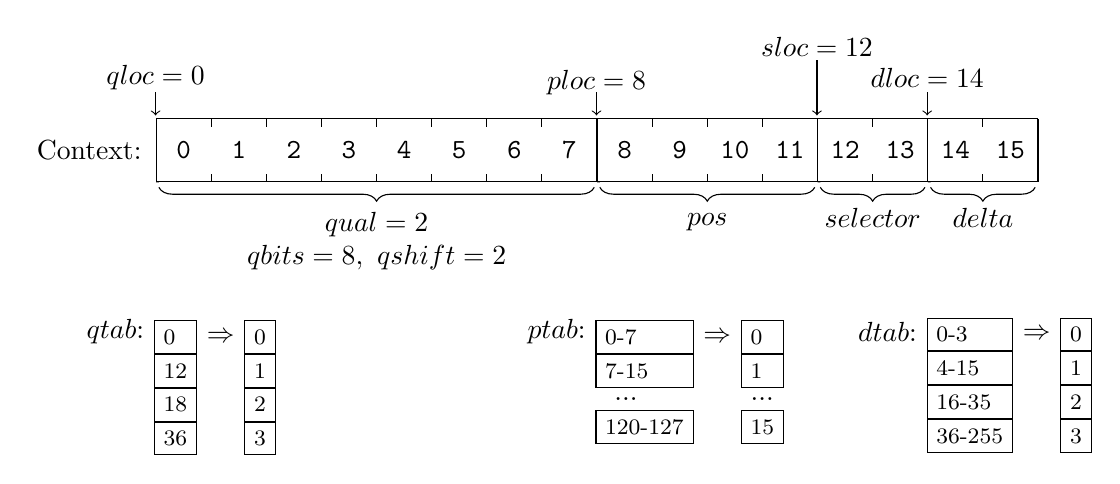
\begin{tikzpicture}[
  boxed/.style={rectangle, draw=black, text width=1cm},
  boxed1/.style={rectangle, draw=black},
  boxed2/.style={rectangle, draw=black, text width=.3cm},
  boxed3/.style={rectangle, draw=black, text width=0.85cm},
]
\newcommand{\x}{0.7cm}
\node at (-0.5, 0) {Context:};
\draw[-] (0*\x+.5*\x,-0.4) -- (0*\x+.5*\x,+0.4);
\foreach \w/\i [count=\n] in {
  3/0, 3/1, 3/2, 3/3, 3/4, 3/5, 3/6, 0/7,   % qual
  3/8, 3/9, 3/10, 0/11,                     % pos
  3/12, 0/13,                               % selector
  3/14, 0/15} {                             % delta
    \draw[-] (\n*\x+.5*\x,-0.4)  -- (\n*\x+.5*\x,-\w/10);
    \draw[-] (\n*\x+.5*\x,\w/10) -- (\n*\x+.5*\x, 0.4);
    \draw[-] (\n*\x-.5*\x,-0.4)  -- (\n*\x+.5*\x,-0.4);
    \draw[-] (\n*\x-.5*\x, 0.4)  -- (\n*\x+.5*\x, 0.4);
    \node(N\n)[minimum height=1cm,minimum width=\x,xshift=\n*\x,font=\ttfamily](N\n){\i};
}
\draw[<-] ([yshift=1pt]N1.north west)+(0,-0.1cm) -- +(0,0.2cm)
    node[yshift=5pt]{$qloc=0$};
\draw[<-] ([yshift=1pt]N9.north west)+(0,-0.1cm) -- +(0,0.2cm)
    node[yshift=3.5pt]{$ploc=8$};
\draw[<-] ([yshift=1pt]N13.north west)+(0,-0.1cm) -- +(0,0.6cm)
    node[yshift=5pt]{$sloc=12$};
\draw[<-] ([yshift=1pt]N15.north west)+(0,-0.1cm) -- +(0,0.2cm)
    node[yshift=5pt]{$dloc=14$};
\draw[decoration={brace,mirror,amplitude=5pt,raise=2pt, post=moveto, pre length=1pt, post length=1pt},decorate]
  (0.5*\x,-0.4) -- node[below=6pt] {\begin{tabular}{c}$qual \shiftl= 2$\\$qbits=8,\ qshift=2$\end{tabular}} +(8*\x,0);
\draw[decoration={brace,mirror,amplitude=5pt,raise=2pt, post=moveto, pre length=1pt, post length=1pt},decorate]
  (8.5*\x,-0.4) -- node[below=8pt] {$pos$} +(4*\x,0);
\draw[decoration={brace,mirror,amplitude=5pt,raise=2pt, post=moveto, pre length=1pt, post length=1pt},decorate]
  (12.5*\x,-0.4) -- node[below=6pt] {$selector$} +(2*\x,0);
\draw[decoration={brace,mirror,amplitude=5pt,raise=2pt, post=moveto, pre length=1pt, post length=1pt},decorate]
  (14.5*\x,-0.4) -- node[below=6pt] {$delta$} +(2*\x,0);

\node[right] (Q) at ([yshift=-1.8cm,xshift=-1cm]N1.south west) {$qtab$:};
\node[above right,boxed2] (Q0) at (Q.south east)  {\footnotesize{0}};
\node[below right,boxed2] (Q1) at (Q0.south west) {\footnotesize{12}};
\node[below right,boxed2] (Q2) at (Q1.south west) {\footnotesize{18}};
\node[below right,boxed2] (Q3) at (Q2.south west) {\footnotesize{36}};

\node[right] (Qeq) at (Q0.east) {$\Rightarrow$};
\node[      right,boxed1] (q0) at (Qeq.east) {\footnotesize{0}};
\node[below right,boxed1] (q1) at (q0.south west) {\footnotesize{1}};
\node[below right,boxed1] (q2) at (q1.south west) {\footnotesize{2}};
\node[below right,boxed1] (q3) at (q2.south west) {\footnotesize{3}};

%\node[right] (P) at ([xshift=3cm]Q.east) {$ptab$:};
\node[right] (P) at ([yshift=-1.8cm,xshift=-1cm]N9.south west) {$ptab$:};
\node[above right,boxed] (P0)   at (P.south east)  {\footnotesize{0-7}};
\node[below right,boxed] (P8)   at (P0.south west) {\footnotesize{7-15}};
\node[below right]       (P16)  at (P8.south west) {\ ...};
\node[below right,boxed] (P124) at (P16.south west) {\footnotesize{120-127}};

\node[right] (Peq) at (P0.east) {$\Rightarrow$};
\node[      right,boxed2] (p0)   at (Peq.east) {\footnotesize{0}};
\node[below right,boxed2] (p8)   at (p0.south west) {\footnotesize{1}};
\node[below right       ] (p16)  at (p8.south west) {...};
\node[below right,boxed2] (p124) at (p16.south west) {\footnotesize{15}};

%\node[right] (D) at ([xshift=4cm]P.east) {$dtab$:};
\node[right] (D) at ([yshift=-1.8cm,xshift=-1cm]N15.south west) {$dtab$:};
\node[above right,boxed3] (D0) at (D.south east)  {\footnotesize{0-3}};
\node[below right,boxed3] (D1) at (D0.south west) {\footnotesize{4-15}};
\node[below right,boxed3] (D2) at (D1.south west) {\footnotesize{16-35}};
\node[below right,boxed3] (D3) at (D2.south west) {\footnotesize{36-255}};

\node[right] (Ded) at (D0.east) {$\Rightarrow$};
\node[      right,boxed1] (d0) at (Ded.east) {\footnotesize{0}};
\node[below right,boxed1] (d1) at (d0.south west) {\footnotesize{1}};
\node[below right,boxed1] (d2) at (d1.south west) {\footnotesize{2}};
\node[below right,boxed1] (d3) at (d2.south west) {\footnotesize{3}};

\end{tikzpicture}
\end{center}

The entropy encoder used is shared between all models, so the bit
streams are multiplexed together.

The 16-bit quality value context is constructed by adding sub-contexts
together consisting of previous quality values, position along the
current record, a running count (per record) of how many times the
quality value has differed to the previous one (delta), and an
arbitrary stored selector value, each shifted to a defined location
within the combined context value ($qloc$, $ploc$, $dloc$ and
$sloc$ respectively).  The qual, pos and delta sub-contexts are
computed from the previous data while the selector, if used, is read
directly from the compressed data stream.  The selector may be used to
switch parameter sets, or simply to group quality strings into
arbitrary user-defined sub-sets.  The numeric values for each of these
components can be passed through lookup tables ($qtab$ for quality,
$ptab$ for positions, $dtab$ for running delta and $stab$ for turning
the selector $s$ into a parameter index $x$).  These all convert the
monotonically increasing range 0$\rightarrow$M to a (usually smaller)
monotonically increasing 0$\rightarrow$N.  For example if we wish to
use the approximate position along a 100 byte string, we may uniformly
map 0$\rightarrow$127 to 0$\rightarrow$15 to utilise 4 bits of our
16-bit combined context.

As some sequencing instruments produce binned qualities, e.g. 0, 10, 25,
35, these values are squashed to incremental values from 0 to
$max\_sym-1$ where $max\_sym$ is the maximum number of distinct
quality values observed.  If this transform is required, the flag
$have\_qmap$ will be set and a mapping table ($qmap$) will hold the
original quality values.  The decoded qualities will be the smaller
mapped range.

The quality sub-context is constructed by shifting left the previous
quality sub-context by $qshift$ bits and adding the current quality
after passing through the $qmap$ squashing process and if defined
through the $qtab$ lookup table.  The quality context is limited to
$qbits$ long and is added to the combined context starting at bit
$qloc$.  The quality sub-context is reset to zero at the start of each
new record.
\footnote{For example if we have 4 quality values in use -- 0, 10, 25 and
35 -- we will be encoding quality values 0, 1, 2 and 3.  We may wish to
define $qbits$ to be 6 and $qshift$ to be 2 such that the previous 3
quality values can be used as context, for the prediction of the next
quality value.  There will likely be little reason to use $qtab$ in
this scenario, but an encoder could define $qtab$ to convert \{0, 1, 2, 3\}
to \{0, 0, 0, 1\} and use $qshift$ of 1 instead, giving us
knowledge of which of the previous 6 values were maximum quality.}

The position context is simply the number of remaining quality values
in this record, so is a value starting at record length (minus 1) and
decrementing.  As with the quality context it may be passed through a
lookup table $ptab$ before shifting left by $ploc$ bits and adding to
the combined context.

Delta is a count of the number of times the quality value has changed
from one value to a different one.  Thus a run of identical values
will not increase delta.  It gets reset to zero at the start of every
record.  It may be adjusted by the $dtab$ lookup table and is shifted
by $dloc$ before adding to the combined context.

The selector value may also be used as a sub-context, if the $do\_sel$
paramter is set.  The initial context value (reset per record) is
defined within each parameter set, providing a more general purpose
alternative to adding the selector value at a defined location
($sloc$) into the context.

Thus the full context can be updated after each decoded quality with
the following pseudocode.  Note for brevity this is assuming the
$pos$, $delta$, $prevq$, $qctx$ and $sel$ parameters referred are global and updateable.

\begin{algorithmic}[1]
\Function{FQZUpdateContext}{$params, q$}
  \State $ctx \gets params.context$ \Comment{Also the initial value}
  \State $qctx \gets (qctx \shiftl params.qshift) + qtab_q$
  \State $ctx   \gets ctx + ((qctx \bitand (2^{params.qbits}-1)) \shiftl params.qloc)$
  \If{$params.pflags \bitand 32$} \Comment{$have\_ptab$}
    \State $p \gets $\Call{Min}{$pos$, $1023$}
    \State $ctx \gets ctx + (ptab_p \shiftl params.ploc)$
  \EndIf
  \If{$params.pflags \bitand 64$} \Comment{$have\_dtab$}
    \State $d \gets $\Call{Min}{$delta$, $255$}
    \State $ctx \gets ctx + (dtab_d \shiftl params.dloc)$
    \If{$prevq \ne q$}
      \State $delta \gets delta+1$
    \EndIf
    \State $prevq \gets q$
  \EndIf
  \If{$params.pflags \bitand 8$} \Comment{$do\_sel$}
    \State $ctx \gets ctx + (sel \shiftl params.sloc)$
  \EndIf
  \State \Return $ctx\bitand (2^{16}-1)$
\EndFunction
\end{algorithmic}

In summary context is produced using the following models:

\begin{table}[h]
\centering
\begin{tabular}{lrlp{9cm}}
 Model & Max symbol & Context size & Description\\
\hline
$model\_qual$ & $max\_sym$ & $2^{16}$ & Primary model for quality values \\
$model\_len$  & 256        & 4       & Read length models with the context 0-3 being successive byte numbers (little endian order) \\
$model\_rev$  & 2          & none    & Used if $pflags.do\_rev$ is defined.  Indicating which strings to reverse. \\
$model\_dup$  & 2          & none    & Used if $pflags.do\_dup$ is defined.  Indicates if this whole string is a duplicate of the last one \\
$model\_sel$  & $max\_sel$ & none    & Used if $gflags.multi\_param$ or $pflags.do\_sel$ are defined. \\
\end{tabular}
\end{table}

\pagebreak
\subsection{FQZComp Data Stream}

The start of an FQZComp data stream consists of the parameters used by
the decoder. The data layout is as follows.

\begin{table}
\centering
\begin{tabular}{|r|r|r|r|r|p{8cm}|l|l|}
\hline
\multicolumn{3}{|r|}{\textbf{Bits} }                   & \textbf{Type}  & \textbf{Name}                  & \multicolumn{3}{p{8.8cm}|}{\textbf{Description}} \\
\hline
\multicolumn{3}{|r|}{8}                                & uint8          & $version$                      & \multicolumn{3}{p{8.8cm}|}{FQZComp format version: must be 5}\\
\hline
\multicolumn{3}{|r|}{8}                                & uint8          & $gflags$                       & \multicolumn{3}{p{8.8cm}|}{Global FQZcomp bit-flags. From lowest bit to highest:}\\
\multicolumn{3}{|r|}{}                                 &                &                                & \multicolumn{3}{p{8.8cm}|}{1: $multi\_param$: indicates more than one parameter block is present.  Otherwise set $nparam = 1$} \\
\multicolumn{3}{|r|}{}                                 &                &                                & \multicolumn{3}{p{8.8cm}|}{2: $have\_stab$: indicates the parameter selector is mapped through $stab$.  Otherwise set $stab_i = i$} \\
\multicolumn{3}{|r|}{}                                 &                &                                & \multicolumn{3}{p{8.8cm}|}{4: $do\_rev$: $model\_revcomp$ will be used. (CRAM v3.1)} \\
\hline

\multicolumn{8}{|l|}{}\\[-0.7em]
\multicolumn{8}{|l|}{\textit{If $multi\_param$ gflag is set:} } \\
\cline{2-7}
                       & \multicolumn{2}{r|}{8}        & uint8          & \multicolumn{1}{r|}{$nparam$ } & \multicolumn{2}{p{8.4cm}|}{Number of parameter blocks (defaults to 1)} & \\
\cline{2-7}

\multicolumn{8}{|l|}{}\\[-0.5em]
\multicolumn{8}{|l|}{\textit{If $have\_stab$ gflag is set:} }                                                                                                                                 \\
\cline{2-7}
                       & \multicolumn{2}{r|}{8}        & uint8          & $max\_sel$                     & \multicolumn{2}{p{8.4cm}|}{Maximum parameter selector value} & \\
                       & \multicolumn{2}{r|}{variable} & table          & $stab$                         & \multicolumn{2}{p{8.4cm}|}{Parameter selector table} & \\
\cline{2-7}
\multicolumn{8}{|l|}{}\\
\hline
\hline
\multicolumn{8}{|l|}{}\\[-0.7em]
\multicolumn{8}{|l|}{\textit{Parameter block: repeated $nparam$ times: (selected via $model\_sel$ and $stab$)}} \\
\cline{2-7}
                       & \multicolumn{2}{r|}{16}        & uint16        & $context$                      & \multicolumn{2}{p{8.4cm}|}{Starting context value} & \\
\cline{2-7}
                       & \multicolumn{2}{r|}{8}        & uint8          & $pflags$                       & \multicolumn{2}{p{8.4cm}|}{Per-parameter block bit-flags. From lowest bit to highest:} & \\
                       & \multicolumn{2}{r|}{}         &                &                                & \multicolumn{2}{p{8.4cm}|}{1: Reserved} & \\
                       & \multicolumn{2}{r|}{}         &                &                                & \multicolumn{2}{p{8.4cm}|}{2: $do\_dedup$: model\_dup will be used} & \\
                       & \multicolumn{2}{r|}{}         &                &                                & \multicolumn{2}{p{8.4cm}|}{4: $do\_len$: model\_len will be used for every record.} & \\
                       & \multicolumn{2}{r|}{}         &                &                                & \multicolumn{2}{p{8.4cm}|}{8: $do\_sel$: model\_sel will be used.} & \\
                       & \multicolumn{2}{r|}{}         &                &                                & \multicolumn{2}{p{8.4cm}|}{16: $have\_qmap$: indicates quality map is present} & \\
                       & \multicolumn{2}{r|}{}         &                &                                & \multicolumn{2}{p{8.4cm}|}{32: $have\_ptab$: Load $ptab$, otherwise position contexts are unused} & \\
                       & \multicolumn{2}{r|}{}         &                &                                & \multicolumn{2}{p{8.4cm}|}{64: $have\_dtab$: Load $dtab$, otherwise delta contexts are unused} & \\
                       & \multicolumn{2}{r|}{}         &                &                                & \multicolumn{2}{p{8.4cm}|}{128: $have\_qtab$: Load $qtab$, otherwise set $qtab_i = i$} &\\
\cline{2-7}
                       & \multicolumn{2}{r|}{8}        & uint8          & $max\_sym$                     & \multicolumn{2}{p{8.4cm}|}{Total number of distinct quality values} & \\
\cline{2-7}
                       & \multicolumn{2}{r|}{4}        & uint4 (high)   & $qbits$                        & \multicolumn{2}{p{8.4cm}|}{Total number of bits for quality context} & \\
                       & \multicolumn{2}{r|}{4}        & uint4 (low)    & $qshift$                       & \multicolumn{2}{p{8.4cm}|}{Left bit shift per successive quality in quality context} & \\
                       & \multicolumn{2}{r|}{4}        & uint4 (high)   & $qloc$                         & \multicolumn{2}{p{8.4cm}|}{Bit position of quality context} & \\
                       & \multicolumn{2}{r|}{4}        & uint4 (low)    & $sloc$                         & \multicolumn{2}{p{8.4cm}|}{Bit position of selector context} & \\
                       & \multicolumn{2}{r|}{4}        & uint4 (high)   & $ploc$                         & \multicolumn{2}{p{8.4cm}|}{Bit position of position context} & \\
                       & \multicolumn{2}{r|}{4}        & uint4 (low)    & $dloc$                         & \multicolumn{2}{p{8.4cm}|}{Bit position of delta context }& \\
\cline{2-7}

& \multicolumn{6}{l|}{} & \\[-0.7em]
\multicolumn{1}{|l|}{} & \multicolumn{6}{l|}{ \textit{If $have\_map$ pflag is set:} } & \\
\cline{3-6}
                       &  & variable                   & uint8[$max\_sym$]          & $qmap$             & Map for unbinning quality values. & & \\
\cline{3-6}

& \multicolumn{6}{l|}{} & \\[-0.5em]
\multicolumn{1}{|l|}{} & \multicolumn{6}{l|}{ \textit{If $have\_qtab$ pflag is set:} } & \\
\cline{3-6}
                       &  & variable                   & table          & $qtab$                         & Quality context lookup table & & \\
\cline{3-6}

& \multicolumn{6}{l|}{} & \\[-0.5em]
\multicolumn{1}{|l|}{} & \multicolumn{6}{l|}{ \textit{If $have\_tab$ pflag is set:} } & \\
\cline{3-6}
                       &  & variable                   & table          & $ptab$                         & Position context lookup table & & \\
\cline{3-6}

& \multicolumn{6}{l|}{} & \\[-0.5em]
\multicolumn{1}{|l|}{} & \multicolumn{6}{l|}{ \textit{If $have\_tab$ pflag is set:} } & \\
\cline{3-6}
                       &  & variable                   & table          & $dtab$                         & Delta context lookup table & & \\
\cline{3-6}
& \multicolumn{6}{l|}{} & \\
\cline{2-7}
\multicolumn{8}{|l|}{}\\
\hline
\end{tabular}
\end{table}

% As an example configuration, with 8 distinct quality values we would
% use $qmap$ to encode/decode qualities in the range 0-7 and can do
% Order-3 entropy encoding by setting $qbits=9$ and $qshift=3$.  This
% leaves 7 bits remaining, which would could distribute as 3 bits of
% position (perhaps pos/16 or pos/32 to get approximate location), 3
% bits of running delta/4, and a bit to distinguish READ1 from READ2.
% Disagramatically the combined context layout would look this this:
%
% \includegraphics[width=250pt, keepaspectratio=true]{img/fqz_bits.png}
% FIXME: read2 becomes selector?
%
% In parameter terms we would use these values in the parameter block:
%
% \begin{tabular}{lrl}
% \hline
% \textbf{Field} & \textbf{Value} & \textbf{Note}\\
% \hline
% qbits  & 9  & 3 bit each $\implies$ Order-3 Markov model \\
% qshift & 3  & E.g. HiSeq X 8-binned, as 3 bit qmap \\
% qloc   & 0  & No $qtab$ needed, but $qmap$ converts qual to 0-7 range.\\
% \hline
% ploc   & 9  & With $ptab$ performing pos/32 function.\\
% \hline
% dloc   & 12 & With $dtab$ performing delta/4 function.\\
% \hline
% rloc   & 15 & 1 bit, iff $do\_read2$ flag is set\\
% \hline
% \end{tabular}
%
% FIXME: our worked example should include actual bytes for qmap, ptab
% and dtab too.


\textsc{FQZDecodeParams} below describes the pseudocode for reading
the parameter block.

\begin{algorithmic}[1]
\Procedure{FQZDecodeParams}{}
  \State $vers \gets $\Call{ReadUint8}{}
  \If{$vers \ne 5$}
    \State ERROR
  \EndIf
  \State $gflags \gets$ \Call{ReadUint8}{}
  \If{$gflags \bitand 1$} \Comment{$multi\_param$}
    \State $nparam \gets$ \Call{ReadUint8}{}
    \State $max\_sel \gets nparam$
  \Else
    \State $nparam \gets 1$
    \State $max\_sel \gets 0$
  \EndIf
  \If{$gflags \bitand 2$} \Comment{$have\_stab$}
    \State $max\_sel \gets$ \Call{ReadUint8}{}
    \State $stab \gets$ \Call{ReadArray}{$256$}
  \EndIf
  \State $max\_sym \gets 0$
  \For{$p \gets 0$ to $nparam-1$}
    \State $param_p \gets$ \Call{FQZDecodeSingleParam}{}
    \If {$max\_sym < param_p.max\_sym$}
      \State $max\_sym \gets param_p.max\_sym$ \Comment{Maximum across all param sets}
    \EndIf
  \EndFor
\EndProcedure
\end{algorithmic}

\begin{algorithmic}[1]
\Function{FQZDecodeSingleParam}{}
  \settowidth{\maxwidth}{p.have\_qtab\ }
  \State \algalign{p.context}{\gets} \Call{ReadUint16}{}
  \State \algalign{p.flags}{\gets} \Call{ReadUint8}{}
%  \State \algalign{have\_qtab}{\gets}    $p.flags\bitand 128$
%  \State \algalign{have\_dtab}{\gets}    $p.flags\bitand 64$
%  \State \algalign{have\_ptab}{\gets}    $p.flags\bitand 16$
%  \State \algalign{do\_rev}{\gets}    $flags\bitand 16$
%  \State \algalign{do\_sel}{\gets} $flags\bitand 8$
%  \State \algalign{do\_len}{\gets}    $flags\bitand 4$
%  \State \algalign{do\_dedup}{\gets}  $flags\bitand 2$
%  \State \algalign{have\_qmap}{\gets}   $flags\bitand 1$
  \State \algalign{p.max\_sym}{\gets} \Call{ReadUint8}{}
  \State \algalign{p.first\_len}{\gets} $1$

  \settowidth{\maxwidth}{p.qshift\ }
  \State \algalign{x}{\gets} \Call{ReadUint8}{}
  \State \algalign{p.qbits}{\gets} $x \bdiv 16$
  \State \algalign{p.qshift}{\gets} $x \bmod 16$
  \State \algalign{x}{\gets} \Call{ReadUint8}{}
  \State \algalign{p.qloc}{\gets} $x \bdiv 16$
  \State \algalign{p.sloc}{\gets} $x \bmod 16$
  \State \algalign{x}{\gets} \Call{ReadUint8}{}
  \State \algalign{p.ploc}{\gets} $x \bdiv 16$
  \State \algalign{p.dloc}{\gets} $x \bmod 16$

  \If{$p.flags\bitand 1$} \Comment{Have qmap}
    \For{$i \gets 0$ to $p.max\_sym-1$}
      \State $p.qmap_i \gets$ \Call{ReadUint8}{}
    \EndFor
  \EndIf

  \If{$p.flags\bitand 128$} \Comment{Have qtab}
    \State $p.qtab \gets$ \Call{ReadArray}{$256$}
  \Else
    \For{$i \gets 0$ to $256$}
      \State $p.qtab_i \gets i$
    \EndFor
  \EndIf

  \If{$p.flags\bitand 16$} \Comment{Have ptab}
    \State $p.ptab \gets$ \Call{ReadArray}{$1024$}
  \EndIf

  \If{$p.flags\bitand 64$} \Comment{Have dtab}
    \State $p.qtab \gets$ \Call{ReadArray}{$256$}
  \EndIf

  \State \Return $p$
\EndFunction
\end{algorithmic}

\textsc{FQZCreateModels} creates the decoder models based on the above
parameters and the shared range coder.

\begin{program}[H]
\begin{algorithmic}[1]
\Procedure{FQZCreateModels}{}
  \State $rc \gets $\Call{RangeDecodeCreate}{}
  \For{$i \gets 0$ to $3$}
    \State $model\_len_i \gets $\Call{ModelCreate}{$256$}
  \EndFor
  \For{$i \gets 0$ to $2^{16}-1$}
    \State $model\_qual_i \gets $\Call{ModelCreate}{$max\_sym+1$}
  \EndFor
  \State $model\_dup \gets $\Call{ModelCreate}{$2$}
  \State $model\_rev \gets $\Call{ModelCreate}{$2$}
  \If{$max\_sel > 0$}
    \State $model\_sel \gets $\Call{ModelCreate}{$max\_sel+1$}
  \EndIf
\EndProcedure
\end{algorithmic}
\end{program}

\textsc{ReadArray} reads an array $A$ of size $n$ which maps values 0
to $n-1$ to a smaller range (0 to $m-1$), both monotonically
increasing.  For efficiency this is done using a two-level run length
encoding.

Assuming $m < n$ there will be runs of the same value.  We measure run
lengths for all values (even if they are zero).  For example an array
$A = \{0,1,3,4,5,6,7,7,7,7\}$ may be converted to run lengths $R =
\{1,1,0,1,1,1,1,4\}$.  To keep values in this array fitting within one
byte, long runs are broken down in a successive series of 255 values,
so a run of length 600 becomes 255 255 90.

This array $R$ is no longer monotonically increasing but may still
have repeated values, so is run-length encoded by storing the number
of additional values whenever the last two lengths match.  This
converts $R$ to $R2 = \{1, 1, +0, 0, 1, 1, +2, 4\}$ where the `+'
symbol is shown purely to indicate the values representing the
additional run-length copy numbers.  (This also now turns the example
run of 600 above into 255 255 0 90.)

The final array $R2$ is the stored data stream.  The decoder process
is the reverse of the above, starting by converting $R2$ to $R$ and
then $A$.  The following pseudocode demonstrates this process.

\begin{algorithmic}[1]
\Function{ReadArray}{n}
\State $i,j,z \gets 0$
\State $last \gets -1$
\While{$z < n$} \Comment{Convert $R2$ to $R$}
  \State $run \gets $ \Call{ReadUint8}{}
  \State $R_j \gets run$
  \State $j \gets j+1$
  \State $z \gets z + run$
  \If{$run = last$}
    \State $copy \gets $ \Call{ReadUint8}{}
    \For{$x \gets 1 $ to $copy$}
      \State $R_j \gets run$
      \State $j \gets j+1$
    \EndFor
    \State $z \gets z + run \times copy$
  \EndIf
  \State $last \gets run$
\EndWhile
\Statex
\State $i,j,z \gets 0$
\While{$z < n$} \Comment{Convert $R$ to $A$}
  \State $run\_len \gets 0$
  \Repeat
    \State $part \gets R_j$
    \State $j \gets j + 1$
    \State $run\_len \gets run\_len + part$
  \Until{$part \ne 255$}
  \For{$x \gets 1 $ to $run\_len$}
    \State $A_z \gets i$
    \State $z \gets z+1$
  \EndFor
  \State $i \gets i+1$
\EndWhile
\Statex
\State \Return $A$
\EndFunction
\end{algorithmic}

The main loop decodes data in the following order per read:  read
length (if not fixed), the flag for whether this is read 2 (if
needed), a bit flag to indicate if the quality is duplicated (if
needed), followed by record length number of quality values using
various data gathered since the start of this read as context.

The output of this function is an array of quality values in the
variable $output$, indexed with the $i^{th}$ value via $output_i$.
The output buffer is a concatenation of all quality values for each
record.  The record lengths are recorded, but note this is the number
of qualities encoded in CRAM for this sequence record and this does
not necessarily have to match the number of base calls (for example
where qualities are explicitly specified for SNP bases but not
elsewhere).

\algnewcommand{\algorithmicgoto}{\textbf{go to}}%
\algnewcommand{\Goto}[1]{\algorithmicgoto\ \texttt{#1}}%
\algnewcommand{\Label}{\State\unskip}

\begin{algorithmic}[1]
\Function{FQZNewRecord}{}
  \State $sel \gets 0$
  \State $x \gets 0$
  \If{$max\_sel > 0$} \Comment{Find parameter selector}
    \State $sel \gets model\_sel.$\Call{ModelDecode}{$rc$}
    \If{$have\_stab$}
       \State $x \gets stab_{sel}$
    \EndIf
  \EndIf
  \State $param \gets params_x$

  \Statex
  \If{$param.do\_len \logor param.first\_len$} \Comment{Decode read length}
    \State $rec\_len \gets $\Call{DecodeLength}{rc}
    \State $param.last\_len \gets rec\_len$
    \If{$param.do\_len = 0$}
      \State $param.first\_len = 0$
    \EndIf
  \Else
    \State $rec\_len \gets param.last\_len$
  \EndIf
  \State $pos \gets rec\_len$

  \Statex
  \If{$param.do\_rev$} \Comment{Check if needs reversal}
    \State $rev_{rec} \gets model\_rev.$\Call{ModelDecode}{$rc$}
    \State $len_{rec} \gets rec\_len$
  \EndIf
  \State $rec \gets rec+1$

  \Statex
  \State $is\_dup \gets 0$
  \If{$do\_dedup$} \Comment{Duplicate last string if appropriate}
    \If{$model\_dup.$\Call{ModelDecode}{$rc$} > 0}
      \State $is\_dup \gets 1$
    \EndIf
  \EndIf
  \Statex
  \State $qctx \gets 0$
  \State $delta \gets 0$
  \State $prevq \gets 0$
  \State \Return $x$\Comment{Tabulated parameter selector}
\EndFunction
\end{algorithmic}

\begin{algorithmic}[1]
\Procedure{FQZDecode}{}
  \State $buf\_len \gets$ \Call{ReadUint7}{}
  \State \Call{FQZDecodeParams}{}
  \State \Call{FQZCreateModels}{}
  \State $i \gets 0$\Comment{Position in total quality block}
  \State $pos \gets 0$\Comment{Remaining base count current quality string}
  \Label \texttt{next\_record:}
  \While{$i < buf\_len$}
    \If{$pos = 0$}\Comment{Reset state at start of each new record}
      \State $x \gets $\Call{FQZNewRecord}{}
      \If {$is\_dup = 1$}
        \For{$j \gets 0$ to $rec\_len-1$}
          \State $output_{i+j} \gets output_{i+j-rec\_len}$
        \EndFor
        \State $i \gets i+rec\_len$
        \State $pos \gets 0$
        \State \Goto{next\_record}
      \EndIf

      \Statex
      \State $param \gets params_x$
      \State $ctx \gets param.context$
    \EndIf
    \Statex
    \State $q \gets model\_qual_{ctx}.$\Call{ModelDecode}{$rc$}
    \Comment{Decode a single quality value}
    \If{$param.have\_qmap$}
      \State $output_i \gets qmap_q$
    \Else
      \State $output_i \gets q$
    \EndIf
    \Statex
    \State $ctx \gets $\Call{FQZUpdateContext}{$param, q$}\Comment{Also updates qlast, prevq and delta}
    \Statex
    \State $i \gets i + 1$
    \State $pos \gets pos - 1$
  \EndWhile
  \If{$do\_rev$}
    \State \Call{ReverseQualities}{$output,\ buf\_len,\ rev,\ len$}
  \EndIf
\EndProcedure
\end{algorithmic}

Read lengths are encoded as 4 8-bit bytes, each having its own model.

\begin{algorithmic}[1]
\Function{DecodeLength}{rc}
\State $rec\_len \gets model\_len_0.$\Call{ModelDecode}{$rc$}
\State $rec\_len \gets rec\_len + (model\_len_1.$\Call{ModelDecode}{$rc$}$ \shiftl 8)$
\State $rec\_len \gets rec\_len + (model\_len_2.$\Call{ModelDecode}{$rc$}$ \shiftl 16)$
\State $rec\_len \gets rec\_len + (model\_len_3.$\Call{ModelDecode}{$rc$}$ \shiftl 24)$
\State \Return $rec\_len$
\EndFunction
\end{algorithmic}

For CRAM v4.0 quality values are stored in their original FASTQ
orientation.  For CRAM v3.1 they are stored in their alignment
orientation and it may be beneficial for compression purposes to
reverse them first.  If so $do\_rev$ will be set and the
\textsc{ReverseQualities} procedure called below after decoding.

\begin{algorithmic}[1]
\Procedure{ReverseQualities}{$qual,\ qual\_len,\ rev,\ len$}
\State $rec \gets 0$
\State $i \gets 0$
\While{$i < qual\_len$}
  \If{$rev_{rec} \ne 0$}
    \State $j \gets 0$
    \State $k \gets len_{rec}-1$
    \While{$j < k$}
      \State \Call{Swap}{$qual_{i+j}$, $qual_{i+k}$}
      \State $j \gets j+1$
      \State $k \gets k-1$
    \EndWhile
    \State $i \gets i + len_{rec}$
    \State $rec \gets rec+1$
  \EndIf
\EndWhile
\EndProcedure
\end{algorithmic}




\end{document}

\title{CRAM codec specification (version 3.1)}
\author{samtools-devel@lists.sourceforge.net}
\date{\headdate}
\maketitle


\begin{quote}\small
The master version of this document can be found at
\url{https://github.com/samtools/hts-specs}.\\
This printing is version~\commitdesc\ from that repository,
last modified on the date shown above.
\end{quote}

\begin{center}
\textit{license: Apache 2.0}
\end{center}
\vspace*{1em}

\newlength{\maxwidth}
\algnewcommand\algorithmicto{\text{ \textbf{to} }}
\algnewcommand\algorithmicin{\text{ \textbf{in} }}
\newcommand{\algalign}[2] % #1 = text to left, #2 = text to right
{\makebox[\maxwidth][l]{$#1{}$}${}#2$}
\algblockdefx[Foreach]{Foreach}{EndForeach}[1]{\textbf{foreach} #1 \textbf{do}}{\textbf{end foreach}}

\makeatletter
\newcommand*{\bdiv}{%
  \nonscript\mskip-\medmuskip\mkern5mu%
  \mathbin{\operator@font div}\penalty900\mkern5mu%
  \nonscript\mskip-\medmuskip
}
\newcommand*{\bitand}{%
  \nonscript\mskip-\medmuskip\mkern5mu%
  \mathbin{\operator@font AND}\penalty900\mkern5mu%
  \nonscript\mskip-\medmuskip
}
\newcommand*{\logand}{% keyword rather than mathematical operator
  \nonscript\mskip-\medmuskip\mkern5mu%
  \mathbin{\operator@font \textbf{and}}\penalty900\mkern5mu%
  \nonscript\mskip-\medmuskip
}
\newcommand*{\logor}{% keyword rather than mathematical operator
  \nonscript\mskip-\medmuskip\mkern5mu%
  \mathbin{\operator@font \textbf{or}}\penalty900\mkern5mu%
  \nonscript\mskip-\medmuskip
}
\newcommand*{\bitor}{%
  \nonscript\mskip-\medmuskip\mkern5mu%
  \mathbin{\operator@font OR}\penalty900\mkern5mu%
  \nonscript\mskip-\medmuskip
}
\newcommand*{\bitxor}{%
  \nonscript\mskip-\medmuskip\mkern5mu%
  \mathbin{\operator@font XOR}\penalty900\mkern5mu%
  \nonscript\mskip-\medmuskip
}
\newcommand\concat{\mathbin{+\mkern-10mu+\,}}
% \newcommand\concat{\mathbin{\oplus\,}}
% \newcommand\concat{\mathbin{\widetilde{+}\,}}
\newcommand\shiftl{\mathbin{<\mkern-3mu<\,}}
\newcommand\shiftr{\mathbin{>\mkern-3mu>\,}}
%\newcommand{\concat}{\ensuremath{+\!\!\!\!+\,}}
\makeatother

\section{introduction}

This document covers the compression and decompression algorithms
(codecs) specific to the CRAM format.  All bar the first of these were
introduced in CRAM v3.1.

It does not cover the CRAM format itself.  For that see \url{http://samtools.github.io/hts-specs/}.

\subsection{Pseudocode introduction}

Various parts of this specification are written in a simplistic
pseudocode.  This intentionally does not make explicit use of data
types and has minimal error checking.  The number of operators is kept
to a minimum, but some are necessary and may be language specific.
Due to the lack of explicit data types, we also have different
division operators to symbolise floating point and integer divisions.

The pseudocode doesn't prescribe any particular programming paradigm -
functional, precedural or object oriented - but it does have a few
implicit assumptions.  Variables are considered to be passed between
functions via unspecified means.  For example the Range Coder sets
$range$ and $code$ during creation and these are used during the
decoding steps, but are not explicitly passed in as variables.  We
make the implicit assumption they are simply local variables of the
particular usage of this range coder.  Other than ephemeral loop
counters, we do not reuse variable names so the intention should be
clear.

The exception to the above is occasionally we need to have multiple
instances of a particular data type, such as Order-1 decoding will
have many models.  Here we use an object oriented way of describing
the problem with $instance$.\textsc{Function} notation.

\subsection{Mathematical operators}

\begin{tabular}{rl}
\hline
\textbf{Operator} & \textbf{Description}\\
\hline
$a + b$       & Addition \\
$a - b$       & Subtraction \\
$a \times b$  & Multiplication \\
$a\ /\ b$     & Floating point division $a/b$\\
$a \bdiv b$   & Integer division $a/b$, equivalent to $\lfloor{a/b}\rfloor$\\
$a \bmod b$   & Integer modulo (remainder) $a - b\times(a \bdiv b)$\\
$a = b$       & Compares $a$ and $b$ variables, yielding true if they match, false otherwise\\
$a \gets b$   & Assigns value of $b$ to variable $a$\\
$a \shiftl b$ & Bit-wise left shift $a$ by $b$ bits, shifting in zeros \\
$a \shiftr b$ & Bit-wise right shift $a$ by $b$ bits, shifting in zeros \\
$a \bitand b$ & Bit-wise AND operator, joining values $a$, $b$\\
$a \bitor b$  & Bit-wise OR operator, joining values $a$, $b$\\
$a \logor b$  & Logical OR operator, joining expressions $a$, $b$\\
$a \logand b$ & Logical AND operator, joining expressions $a$, $b$\\
$a \concat b$ & String concatenation of $a$ and $b$: $ab$.\\
$V_i$         & Element $i$ of vector $V$.\\
              & The entire vector $V$ may be passed into a function.\\
$W_{i,j}$      & Element $i,j$ of two-dimensional vector $W$.\\
              & The entire vector $W$ or a one dimensional slice $W_i$ (of size $j$) may be passed into a function.\\
\hline
\end{tabular}

Note that string concatenation with the $\concat$ operator
assumes the left and right values are converted to string form.  For
example ``level'' $\concat 42$ will convert the integer 42 to ``42''
and produce the string ``level42''.

\subsection{Implicit functions}

\begin{tabular}{rl}
\hline
\textbf{Operator} & \textbf{Description}\\
\hline
\textsc{Min}$(a,\ b)$ & Smaller of $a$ and $b$\\
\textsc{Max}$(a,\ b)$ & Larger of $a$ and $b$\\
\textsc{ReadUint8} & Read an 8-bit unsigned integer (1 byte) from unspecified input source\\
\textsc{ReadUint32} & Read a 32-bit unsigned little-endian integer from unspecified input source\\
\textsc{ReadUint8}$(src)$ & Read an 8-bit unsigned integer (1 byte) from input $src$\\
\textsc{ReadUint32}$(src)$ & Read a 32-bit unsigned little-endian integer from input $src$\\
\textsc{ReadData}$(len)$ & Read $len$ bytes (8-bit unsigned) from an unspecified input source\\
\textsc{ReadData}$(len, src)$ & Read $len$ bytes (8-bit unsigned) from input $src$\\
\textsc{ReadChar}$(src)$ & Read a single character from input $src$\\
\textsc{ReadString}$(src)$ & Read a nul-terminated string from input $src$\\
\textsc{EOF} & Returns true if the input source is exhausted.\\
\textsc{Char}$(a)$ & Converts integer $a$ to a single character of appropriate ASCII value\\
\textsc{Length}$(a)$ & Returns length of string $a$ excluding any nul-termination bytes\\
\textsc{Swap}$(a,\ b)$ & Swaps the contents of $a$ and $b$ variables\\
\hline
\end{tabular}

Many of the input functions here and below are defined to read either
from an unspecified input source (such as the input file descriptor,
or a global buffer that has not been explicitly stated in the
pseudocode), but also have forms that may decode from specified inputs
/ buffers.  They both consume their input sources in the same manner,
using an implicit offset of how many bytes so far have been read.

\subsection{Other basic functions}

\begin{algorithmic}[1]
\Statex
\Statex \textit{Read a variable sized unsigned integer 7-bits at a time.}
\Statex \textit{Returns the value and number of bytes read, but caller is permitted to only use value in assignments.}
\Function{ReadUint7}{$source$} \Comment{If $source$ is unspecified then it is the default input stream}
  \State $value \gets 0$
  \State $length \gets 0$
  \Repeat
    \State $c \gets$ \Call{ReadUint8}{}
    \State $value \gets (value \shiftl 7) + (c \bitand 127)$
    \State $length \gets length + 1$
  \Until{$c < 128$}
  \State \Return ($value$, $length$) \Comment{or just $value$ if caller uses only that}
  \EndFunction
\end{algorithmic}

\section{rANS 4x8 - Asymmetric Numeral System}

% Lifted over from CRAMv3.tex

This is the rANS format first defined in CRAM v3.0.

rANS is the range-coder variant of the Asymmetric Numerical
System\footnote{J. Duda, \textit{Asymmetric numeral systems: entropy
    coding combining speed of Huffman coding with compression rate of
    arithmetic coding}, \url{http://arxiv.org/abs/1311.2540}}.

The structure of the external rANS codec consists of several
components: meta-data consisting of compression-order, and compressed
and uncompressed sizes; normalised frequencies of the alphabet systems
to be encoded, either in Order-0 or Order-1 context; and the rANS
encoded byte stream itself.

Here "Order" refers to the number of bytes of context used in
computing the frequencies. It will be 0 or 1.  Ignoring punctuation
and space, an Order-0 analysis of English text may observe that `e' is
the most common letter (12-13\%), and that `u' occurs only around 2.5\%
of the time.  If instead we consider the frequency of a letter in the
context of one previous letter (Order-1) then these statistics change
considerably;  we know that if the previous letter was `q' then `e'
becomes a rare letter while `u' is the most likely.

These observed frequencies are directly related to the amount of
storage required to encode a symbol (e.g. an alphabet
letter)\footnote{ C.E. Shannon, \textit{A Mathematical Theory of
    Communication}, Bell System Technical Journal, vol. 27,
    pp. 379-423, 623-656, July, October, 1948}.


\subsubsection*{\textbf{rANS 4x8 compressed data structure}}
A compressed data block consists of the following logical parts:

\begin{tabular}{|l|l|>{\raggedright}p{100pt}|>{\raggedright}p{220pt}|}
\hline
\textbf{Value data type} & \textbf{Name} & \textbf{Description}\tabularnewline
\hline
byte & order & the order of the codec, either 0 or 1\tabularnewline
\hline
int & compressed size & the size in bytes of frequency table and compressed blob\tabularnewline
\hline
int & data size & raw or uncompressed data size in bytes\tabularnewline
\hline
byte[] & frequency table & byte frequencies of input data written using RLE\tabularnewline
\hline
byte[] & compressed blob & compressed data\tabularnewline
\hline
\end{tabular}

\subsection{\textbf{Frequency table}}

The alphabet used here is simply byte values, so a maximum of 256
symbols as some values may not be present.

The symbol frequency table indicates which symbols are present and
what their relative frequencies are.  The total sum of symbol
frequencies are normalised to add up to 4095.

Formally, this is an ordered alphabet $\mathbb{A}$ containing symbols $s$ where
$s_{i}$ with the $i$-th symbol in $\mathbb{A}$, occurring with the frequency $freq_{i}$.

\subsubsection*{Order-0 encoding}

The normalised symbol frequencies are then written out as \{symbol,
frequency\} pairs in ascending order of symbol (0 to 255 inclusive).
If a symbol has a frequency of 0 then it is omitted.

To avoid storing long consecutive runs of symbols if all are present
(eg a-z in a long piece of English text) we use run-length-encoding on
the alphabet symbols.  If two consecutive symbols have non-zero
frequencies then a counter of how many other non-zero frequency
consecutive symbols is output directly after the second consecutive
symbol, with that many symbols being subsequently omitted.

For example for non-zero frequency symbols `a', `b', `c', `d' and `e'
we would write out symbol `a', `b' and the value 3 (to indicate `c',
`d' and `e' are also present).

The frequency is output after every symbol (whether explicit or
implicit) using ITF8 encoding. This means that frequencies 0-127 are
encoded in 1 byte while frequencies 128-4095 are encoded in 2 bytes.

Finally the symbol 0 is written out to indicate the end of the
symbol-frequency table.

As an example, take the string \texttt{abracadabra}.

\begin{minipage}[t]{0.5\textwidth}
Symbol frequency:
\\[8pt]
\begin{tabular}{ |r|r| }
\hline
Symbol & Frequency\\
\hline
a & 5 \\
b & 2 \\
c & 1 \\
d & 1 \\
r & 2 \\
\hline
\end{tabular}
\end{minipage}
\begin{minipage}[t]{0.5\textwidth}
Normalised to sum to 4095:
\\[8pt]
\begin{tabular}{ |r|r|}
\hline
Symbol & Frequency\\
\hline
a & 1863 \\
b &  744 \\
c &  372 \\
d &  372 \\
r &  744 \\
\hline
\end{tabular}
\end{minipage}

Encoded as:
\begin{verbatim}
0x61      0x87 0x47      # `a'           <1863>
0x62 0x02 0x82 0xe8      # `b' <+2: c,d>  <744>
          0x81 0x74      # `c' (implicit) <372>
          0x81 0x74      # `d' (implicit) <372>
0x72      0x82 0xe8      # `r'            <744>
0x00                     # <0>
\end{verbatim}


\subsubsection*{Order-1 encoding}

To encode Order-1 statistics typically requires a larger table as for
an $N$ sized alphabet we need to potentially store an $N$x$N$ matrix.
We store these as a series of Order-0 tables.

We start with the outer context byte, emitting the symbol if it is
non-zero frequency.  We perform the same run-length-encoding as we
use for the Order-0 table and end the contexts with a nul byte.  After
each context byte we emit the Order-0 table relating to that context.

One last caveat is that we have no context for the first byte in the
data stream (in fact for 4 equally spaced starting points, see
``interleaving" below).  We use the ASCII value (`\textbackslash0') as
the starting context and so need to consider this in our frequency
table.

Consider \texttt{abracadabraabracadabraabracadabraabracadabra} as
example input.

\begin{minipage}[t]{0.5\textwidth}
Observed Order-1 frequencies:
\\[8pt]
\begin{tabular}{ |r|r|r| }
\hline
Context & Symbol & Frequency\\
\hline
\textbackslash0 & a & 4 \\
\hline
a & a & 3 \\
  & b & 8 \\
  & c & 4 \\
  & d & 4 \\
\hline
b & r & 8 \\
\hline
c & a & 4 \\
\hline
d & a & 4 \\
\hline
r & a & 8 \\
\hline
\end{tabular}
\end{minipage}
\begin{minipage}[t]{0.5\textwidth}
Normalised (per Order-0 statistics):
\\[8pt]
\begin{tabular}{ |r|r|r|}
\hline
Context & Symbol & Frequency\\
\hline
\textbackslash0 & a & 4095 \\
\hline
a & a &  646 \\
  & b & 1725 \\
  & c &  862 \\
  & d &  862 \\
\hline
b & r & 4095 \\
\hline
c & a & 4095 \\
\hline
d & a & 4095 \\
\hline
r & a & 4095 \\
\hline
\end{tabular}
\end{minipage}


Encoded as:
\begin{verbatim}
0x00                 # `\0' context
0x61      0x8f 0xff  # a  <4095>
0x00                 # end of Order-0 table

0x61                 # `a' context
0x61      0x82 0x86  # a            <646>
0x62 0x02 0x86 0xbd  # b <+2: c,d> <1725>
          0x83 0x5e  # c (implicit) <862>
          0x83 0x5e  # d (implicit) <862>
0x00                 # end of Order-0 table

0x62 0x02            # `b' context, <+2: c, d>
0x72      0x8f 0xff  # r <4095>
0x00                 # end of Order-0 table

                     # `c' context (implicit)
0x61      0x8f 0xff  # a <4095>
0x00                 # end of Order-0 table

                     # `d' context (implicit)
0x61      0x8f 0xff  # a <4095>
0x00                 # end of Order-0 table

0x72                 # `r' context
0x61      0x8f 0xff  # a <4095>
0x00                 # end of Order-0 table

0x00                 # end of contexts
\end{verbatim}


\subsection{rANS entropy encoding}

The encoder takes a symbol $s$ and a current state $x$ (initially zero) to
produce a new state $x'$ with function $C$.

{
\setlength{\parindent}{1cm}
\indent $x' = C(s,x)$
}

The decoding function $D$ is the inverse of $C$ such that $C(D(x)) = x$.

{
\setlength{\parindent}{1cm}
\indent $D(x') = (s,x)$
}

The entire encoded message can be viewed as a series of nested $C$
operations, with decoding yielding the symbols in reverse order, much
like popping items off a stack.  This is where the asymmetric part of
ANS comes from.

As we encode into $x$ the value will grow, so for efficiency we ensure
that it always fits within known bounds. This is governed by

{
\setlength{\parindent}{1cm}
\indent $L \leq x < bL-1$
}


where $b$ is the base and $L$ is the lower-bound.

We ensure this property is true before every use of $C$ and after every
use of $D$.  Finally to end the stream we flush any remaining data out
by storing the end state of $x$.


\textbf{Implementation specifics}

We use an unsigned 32-bit integer to hold $x$. In encoding it is
initialised to zero. For decoding it is read little-endian from the
input stream.

Recall $freq_{i}$ is the frequency of the $i$-th symbol $s_{i}$ in alphabet
$\mathbb{A}$.  We define $cfreq_i$ to be cumulative frequency of all symbols
up to but not including $s_{i}$:

{
\setlength{\parindent}{1cm}
$ cfreq_{i} = \left\{
\begin{array}{l l}
0 & \quad \textrm{if $i < 1$} \\
cfreq_{i-1} + freq_{i-1} & \quad \textrm{if $i \geq 1$}
\end{array}
\right. $
% \\*[8pt]
% \indent $cfreq_{i} = \displaystyle \sum_{j=0}^{i-1} freq_j$
}


We have a reverse lookup table $cfreq\_to\_sym_c$ from 0 to 4095
(0xfff) that maps a cumulative frequency $c$ to a symbol $s$.

{
\setlength{\parindent}{1cm}
\indent   $cfreq\_to\_sym_c = s_{i} \quad where \quad c: \enskip cfreq_i \leq c <
cfreq_i + freq_i$
% \\*[8pt]
% \indent   $cfreq\_to\_sym_c = s_{i} ,
% \quad \forall c \in [cfreq_i, cfreq_i + freq_i)$
}


The $x' = C(s,x)$ function used for the ${i}-th symbol ${s} is:

{
\setlength{\parindent}{1cm}
\indent    $x' = (x/freq_i) \times \mathtt{0x1000} + cfreq_i + (x \bmod freq_i)$
}

The $D(x') = (s,x)$ function used to produce the $i$-th symbol $s$ and
a new state $x$ is:

{
\setlength{\parindent}{1cm}
\indent    $c = x' \bitand \mathtt{0xfff}$\\*
\indent    $s_{i} = cfreq\_to\_sym_{c}$\\*
\indent    $x = freq_{i} (x' / \mathtt{0x1000}) + c - cfreq_{i}$
}

Most of these operations can be implemented as bit-shifts and bit-AND,
with the encoder modulus being implemented as a multiplication by the
reciprocal, computed once only per alphabet symbol.

We use $L = \mathtt{0x800000}$ and $b = 256$, permitting us to flush out one byte
at a time (encoded and decoded in reverse order).

Before every encode $C(s,x)$ we renormalise $x$, shifting out the bottom 8
bits of $x$ until $x < \mathtt{0x80000} \times freq_i$.  After finishing encoding we
flush 4 more bytes (lowest 8-bits first) from $x$.

After every decoded $D(x')$ we renormalise $x'$, shifting in the bottom 8
bits until $x \geq \mathtt{0x800000}$.


\subsubsection*{Interleaving}

For efficiency, we interleave 4 separate rANS codecs at the same
time\footnote{F. Giesen, \textit{Interleaved entropy coders},
  \url{http://arxiv.org/abs/1402.3392}}.  For the Order-0 codecs these
simply encode or decode the 4 neighbouring bytes in cyclic fashion
using interleaved codec 1, 2, 3 and 4, sharing the same output buffer
(so the output bytes get interleaved).

For the Order-1 codec we cannot do this as we need to know the
previous byte value as the context for the next byte.  Therefore split
the input data into 4 approximately equal sized
fragments\footnote{This was why the `\textbackslash0' $\to$ `a'
  context in the example above had a frequency of 4 instead of 1.}
starting at $0$, $\lfloor{}len/4\rfloor{}$,
$\lfloor{}len/4\rfloor{}\times2$ and $\lfloor{}len/4\rfloor{}\times 3$.  Each
Order-1 codec operates in a cyclic fashion as with Order-0, all
starting with 0 as their state and sharing the same output buffer. Any
remainder, when the input buffer is not divisible by 4, is processed at
the end by the 4th rANS state.

We do not permit Order-1 encoding of data streams smaller than 4
bytes.

\newpage
\subsection{rANS decode pseudocode}

A na\"ive implementation of a rANS decoder, follows.
This pseudocode is for clarity only and is not expected to be performant and we would normally rewrite this to use lookup tables for maximum efficiency.
The function \textsc{ReadUint8} below is undefined, but is expected to fetch the next single unsigned byte from an unspecified input source.  Similarly for \textsc{ReadITF8} (variable size inetger) and \textsc{ReadUint32} (32-bit unsigned integer in little endian format).

\vskip 0.5cm

\begin{algorithmic}[1]
\Procedure{RansDecode}{$input,\ output$}
\settowidth{\maxwidth}{$n\_out$}
\State \algalign{order}{\gets} \Call{ReadUint8}{}\Comment{Implicit read from $input$}
\State \algalign{n\_in}{\gets} \Call{ReadUint32}{}
\State \algalign{n\_out}{\gets} \Call{ReadUint32}{}
\State \If{$order = 0$}
  \State \Call{RansDecode0}{$output,\ n\_out$}
\Else
  \State \Call{RansDecode1}{$output,\ n\_out$}
\EndIf
\EndProcedure
\end{algorithmic}


\subsubsection*{rANS order-0}

The Order-0 code is the simplest variant.
Here we also define some of the functions for manipulating the rANS state, which are shared between Order-0 and Order-1 decoders.

\vskip 0.5cm

\begin{algorithmic}[1]
\Statex (Reads a table of Order-0 symbol frequencies $F_i$
\Statex (and sets the cumulative frequency table $C_{i+1} = C_i+F_i$)
\Procedure{ReadFrequencies0}{$F, C$}
\State $s \gets$ \Call{ReadUint8}{}\Comment{Next alphabet symbol}
\State $last\_sym \gets s$
\State $rle \gets 0$
\Repeat
  \State $f \gets$ \Call{ReadITF8}{}
  \settowidth{\maxwidth}{$C_s$}
  \State \algalign{F_s}{\gets} $f$
  \If{$rle > 0$}
    \settowidth{\maxwidth}{rle\ }
    \State \algalign{rle}{\gets} $rle-1$
    \State \algalign{s}{\gets} $s+1$
  \Else
    \State $s \gets$ \Call{ReadUint8}{}
    \If{$s = last\_sym+1$}
      \State $rle \gets$ \Call{ReadUint8}{}
    \EndIf
  \EndIf
  \State $last\_sym \gets s$
\Until {$s = 0$}
\Statex \quad\ (Compute cumulative frequencies $C_i$ from $F_i$)
\State $C_0 \gets 0$
\For{$s\gets 0 \algorithmicto 255$}
  \State $C_{s+1} \gets C_s + F_s$
\EndFor
\EndProcedure

\Statex
\Statex (Bottom 12 bits of our rANS state $R$ are our frequency)
\Function{RansGetCumulativeFreq}{$R$}
  \State \Return $R\ \bitand$ 0xfff
\EndFunction
\Statex
\Statex (Convert frequency to a symbol. Find $s$ such that $C_s \le f < C_{s+1}$)
\Statex (We would normally implement this via a lookup table)
\Function{RansGetSymbolFromFreq}{$C, f$}
  \State $s \gets 0$
  \While{$f >= C_{s+1}$}
    \State $s \gets s+1$
  \EndWhile
  \State \Return $s$
\EndFunction
\Statex
\Statex (Compute the next rANS state $R$ given frequency $f$ and cumulative freq $c$)
\Function{RansAdvanceStep}{$R, c, f$}
  \State \Return $f \times (R \shiftr 12) + (R\ \bitand$ 0xfff$) - c$
\EndFunction
\Statex
\Statex (If too small, feed in more bytes to the rANS state $R$)
\Function{RansRenorm}{$R$}
  \While{$R < (1 \shiftl 23)$}
    \State $R \gets (R \shiftl 8) +$\ \Call{ReadUint8}{}
  \EndWhile
  \State \Return $R$
\EndFunction
\Statex
\Procedure{RansDecode0}{$output$, $nbytes$}
  \State \Call{ReadFrequencies0}{$F, C$}
  \For{$j\gets 0 \algorithmicto 3$}
    \State $R_j \gets$ \Call{ReadUint32}{}\Comment{Unsigned 32-bit little endian}
  \EndFor
  \For{$i\gets 0 \algorithmicto nbytes-1$}
    \State $j \gets i \bmod 4$
    \State $f \gets$ \Call{RansGetCumulativeFreq}{$R_j$}
    \State $s \gets$ \Call{RansGetSymbolFromFreq}{$C,\ f$}
    \State $output_i \gets s$
    \State $R_j \gets$\ \Call{RansAdvanceStep}{$R_j,\ C_s,\ F_s$}
    \State $R_j \gets$\ \Call{RansRenorm}{$R_j$}
  \EndFor
\EndProcedure
\end{algorithmic}

\subsubsection*{rANS order-1}

As described above, the decode logic is very similar to rANS Order-0 except we have a two dimensional array of frequencies to read and the decode uses the last character as the context for decoding the next one.
In the pseudocode we demonstrate this by using two dimensional vectors $C_{i,j}$ and $F_{i,j}$.
For simplicity, we reuse the Order-0 code by referring to $C_i$ and $F_i$ of the 2D vectors to get a single dimensional vector that operates in the same manner as the Order-0 code.
This is not necessarily the most efficient implementation.

Note the code for dealing with the remaining bytes when an output buffer is not an exact multiple of 4 is less elegant in the Order-1 code.
This is correct, but it is unfortunately a design oversight.

\vskip 0.5cm

\begin{algorithmic}[1]
\Statex (Reads a table of Order-1 symbol frequencies $F_{i,j}$
\Statex (and sets the cumulative frequency table $C_{i,j+1} = C_{i,j}+F_{i,j}$)
\Procedure{ReadFrequencies1}{$F, C$}
\State $sym \gets$ \Call{ReadUint8}{}\Comment{Next alphabet symbol}
\State $last\_sym \gets sym$
\State $rle \gets 0$
\Repeat
  \State \Call{ReadFrequencies0}{$F_i, C_i$}
  \If{$rle > 0$}
    \settowidth{\maxwidth}{sym}
    \State \algalign{rle}{\gets} $rle-1$
    \State \algalign{sym}{\gets} $sym+1$
  \Else
    \State $sym \gets$ \Call{ReadUint8}{}
    \If{$sym = last\_sym+1$}
      \State $rle \gets$ \Call{ReadUint8}{}
    \EndIf
  \EndIf
  \State $last\_sym \gets sym$
\Until {$sym = 0$}
\EndProcedure

\Statex
\Procedure{RansDecode1}{$output$, $nbytes$}
  \State \Call{ReadFrequencies1}{$F, C$}
  \For{$j\gets 0 \algorithmicto 3$}
    \State $R_j \gets$ \Call{ReadUint32}{}\Comment{Unsigned 32-bit little endian}
    \State $L_j \gets 0$
  \EndFor
  \State $i \gets 0$
  \While{$i < \lfloor nbytes/4 \rfloor$}
    \For{$j\gets 0 \algorithmicto 3$}
      \State $f \gets$ \Call{RansGetCumulativeFreq}{$R_j$}
      \State $s \gets$ \Call{RansGetSymbolFromFreq}{$C_{L_j},\ f$}
      \State $output_{i + j \times \lfloor nbytes/4 \rfloor} \gets s$
      \State $R_j \gets$\ \Call{RansAdvanceStep}{$R_j,\ C_{L_j,s},\ F_{L_j,s}$}
      \State $R_j \gets$\ \Call{RansRenorm}{$R_j$}
      \State $L_j \gets s$
    \EndFor
    \State $i \gets i+1$
  \EndWhile
  \Statex \ \ \ \ (Now deal with the remainder if buffer size is not a multiple of 4,)
  \Statex \ \ \ \ (using rANS state 3 exclusively.)
  \For{$i \gets i \times 4 \algorithmicto len-1$}
    \State $f \gets$ \Call{RansGetCumulativeFreq}{$R_3$}
    \State $s \gets$ \Call{RansGetSymbolFromFreq}{$C_{L_3},\ f$}
    \State $output_i \gets s$
    \State $R_3 \gets$\ \Call{RansAdvanceStep}{$R_3,\ C_{L_3,s},\ F_{L_3,s}$}
    \State $R_3 \gets$\ \Call{RansRenorm}{$R_3$}
    \State $L_3 \gets s$
  \EndFor
\EndProcedure
\end{algorithmic}

\section{rANS 4x16}

% FIXME: Maybe rANS Nx16 with interleaving size being a parameter, to
% permit SIMD optimisation.

CRAM version 3.1 defines an additional rANS entropy encoder, using
16-bit renormalisation instead of the 8-bit used in CRAM 3.0 and with
inbuilt bit-packing and run-length encoding.  The Order-1 rANS 4x16
encoder has also been modified to use a maximum frequency of 1024
instead of 4096.  This offers better cache performance for the large
Order-1 tables and usually has minimal impact on compression ratio.
(The 4x8 rANS entropy encoder is still available if the reduced
frequency range is a problem.)

Frequencies are now stored using uint7 format instead of ITF8.  The
tables are also stored differently, separating the list of symbols
present in the alphabet (those with frequency greater than zero) from
the frequencies themselves.  For the Order-1 frequency table this list
of symbols is those used in any context, thus we only have one
alphabet recorded for all contexts.  This means in some contexts
some (potentially many) symbols will have zero frequency.  To reduce
the Order-1 table size an additional zero run-length encoding step is
used.  Finally the Order-1 frequencies may optionally be compressed
using the Order-0 rANS 4x16 codec.

Frequencies must always add up to a power of 2, but do not necessarily
have to match the final power of two used in the Order-0 (4096) and
Order-1 (1024) entropy decoder algorithm.  A normalisation step is
applied after reading the frequencies to scale them appropriately.
This is required as the Order-1 frequencies may be scaled differently
for each context.

\subsection{Frequency tables}

\begin{algorithmic}[1]
\Statex (Reads a list of symbols used $A$ in our alphabet)
\Function{ReadAlphabet}{}
\State $s \gets$ \Call{ReadUint8}{}
\State $last\_sym \gets s$
\State $rle \gets 0$
\Repeat
  \State $A \gets (A,s)$ \Comment{Append $s$ to the symbol list $A$}
  \If{$rle > 0$}
    \settowidth{\maxwidth}{rle\ }
    \State \algalign{rle}{\gets} $rle-1$
    \State \algalign{s}{\gets} $s+1$
  \Else
    \State $s \gets$ \Call{ReadUint8}{}
    \If{$s = last\_sym+1$}
      \State $rle \gets$ \Call{ReadUint8}{}
    \EndIf
  \EndIf
  \State $last\_sym \gets s$
\Until {$s = 0$}
\State \Return $A$
\EndFunction
\end{algorithmic}

\vskip 0.5cm

\begin{algorithmic}[1]
\Statex (Reads a table of Order-0 symbol frequencies $F_i$
\Statex (and sets the cumulative frequency table $C_{i+1} = C_i+F_i$)
\Procedure{ReadFrequencies4x16\_0}{$F, C$}
\State $F \gets (0,\ ...)$ \Comment(Set to zero for all $i$)
\State $A \gets$ \Call{ReadAlphabet}{}
\Foreach{$i \algorithmicin A$}
  \State $F_i \gets$ \Call{ReadUint7}{}
\EndForeach
\State
\State \Call{NormaliseFrequencies4x16\_0}{$F,\ 12$}
\State
\State $C_0 \gets 0$
\For{$s\gets 0 \algorithmicto 255$}
  \State $C_{s+1} \gets C_s + F_s$
\EndFor
\EndProcedure
\end{algorithmic}

\begin{algorithmic}[1]
\Statex (Normalises a table of frequencies $F_i$ to sum to a specified power of 2.)
\Procedure{NormaliseFrequencies4x16\_0}{$F$, $bits$}
\State $tot \gets 0$
\For{$i\gets 0 \algorithmicto 255$}
  \State $tot \gets tot + F_i$
\EndFor
\If{$tot = 0 \logor tot = (1 \shiftl bits)$}
  \State \Return
\EndIf
\State
\State $shift \gets 0$
\While{$tot < (1 \shiftl bits)$}
  \State $tot \gets tot*2$
  \State $shift \gets shift+1$
\EndWhile
\State
\For{$i\gets 0 \algorithmicto 255$}
  \State $F_i \gets F_i \shiftl shift$
\EndFor
\EndProcedure
\end{algorithmic}

The Order-1 frequencies also store the complete alphabet of
observed symbols (ignoring context) followed by a table of frequencies for
each symbol in the alphabet.  Given many frequencies will be zero
where a symbol is present in one context but not in others, all zero
frequencies are followed by a run length to omit adjacent zeros.

The order-1 frequency table itself may still be quite large, so is
optionally compressed using the order-0 rANS4x16 codec.  This is
specified in the bottom bit of the first byte.  If this is 1, it is
followed by 7-bit encoded uncompressed and compressed lengths and then
the compressed frequency data.  The pseudocode here differs slightly
to elsewhere as it indicates the input sources, which are either the
uncompressed frequency buffer or the default (unspecified) source.
The top 4 bits of the first byte indicate the number of bits used for
the frequency tables.  Permitted values are 10 and 12.

% Should we just have a generic INPUT buffer so we can use either
% unspecified inputs or specified ones?

\begin{algorithmic}[1]
\Statex (Reads a table of Order-1 symbol frequencies $F_{i,j}$
\Statex (and sets the cumulative frequency table $C_{i,j+1} = C_{i,j}+F_{i,j}$)
\Procedure{ReadFrequencies4x16\_1}{$F, C, bits$}
\State $comp \gets$ \Call{ReadUint8}{}
\State $bits \gets comp \shiftr 4$
\If{$(comp \logand 1) \ne 0$}
  \State $u\_size \gets$ \Call{ReadUint7}{} \Comment{Uncompressed size}
  \State $c\_size \gets$ \Call{ReadUint7}{} \Comment{Compressed size}
  \State $c\_data \gets$ \Call{ReadData}{$c\_size$}
  \State $source \gets$ \Call{RansDecode4x16\_0}{$c\_data$} \Comment{Create $u\_size$ bytes of $source$ from $c\_data$}
\Else
  \State (define $source$ to be the default input stream)
\EndIf
\Statex
\State $F \gets ((0,\ ...),\ ...)$ \Comment(Set to zero for all $i$ and $j$)
\State $A \gets$ \Call{ReadAlphabet}{from $source$}
\Foreach{$i \algorithmicin A$}
  \State $run \gets 0$
  \Foreach{$j \algorithmicin A$}
    \If{$run > 0$}
      \State $run \gets run-1$ \Comment{$F_{i,j}$ is implicitly zero already}
    \Else
      \State $F_{i,j} \gets$ \Call{ReadUint7}{from $source$}
      \If{$F_{i,j} = 0$}
        \State $run \gets$ \Call{ReadUint8}{from $source$}
      \EndIf
    \EndIf
  \EndForeach
  \State \Call{NormaliseFrequencies4x16\_0}{$F_i$, $bits$}
  \State
  \State $C_{i,0} \gets 0$
  \For{$j\gets 0 \algorithmicto 255$}
    \State $C_{i,j+1} \gets C_{i,j} + F_{i,j}$
  \EndFor
\EndForeach
\EndProcedure
\end{algorithmic}

\subsection{rANS 4x16 Order-0}

To decode an Order-0 encoded byte stream we first decode the symbol
frequencies as described above and then decode the 4 interleaved rANS
streams.  This is similar to the old (4x8) rANS decoder, but the
\textsc{RansRenorm} function is replaced by a single 16-bit
renormalisation instead of a loop using 8-bit values.

\begin{algorithmic}[1]
\Function{RansGetCumulativeFreq4x16}{$R, bits$}
  \State \Return $R\ \bitand ((1 \shiftl bits) -1)$
\EndFunction
\Function{RansAdvanceStep4x16}{$R, c, f, bits$}
  \State \Return $f \times (R \shiftr bits) + (R\ \bitand ((1 \shiftl bits) -1) - c$
\EndFunction
\Statex
\Function{RansRenorm4x16}{$source$, $R$}
  \If{$R < (1 \shiftl 15)$}
    \State $R \gets (R \shiftl 16) +$\ \Call{ReadUint16}{$source$}
  \EndIf
  \State \Return $R$
\EndFunction
\Statex
\Function{RansDecode4x16\_0}{$len$}
  \State \Call{ReadFrequencies4x16\_0}{$F$, $C$}
  \For{$j \gets 0 \algorithmicto 3$}
    \State $R_j \gets$ \Call{ReadUint32}{}
  \EndFor
  \For{$i\gets 0 \algorithmicto len-1$}
    \State $j \gets i \bmod 4$
    \State $f \gets$ \Call{RansGetCumulativeFreq4x16}{$R_j,\ 12$}
    \State $s \gets$ \Call{RansGetSymbolFromFreq}{$C,\ f$}
    \State $out_i \gets s$
    \State $R_j \gets$\ \Call{RansAdvanceStep4x16}{$R_j,\ C_s,\ F_s,\ 12$}
    \State $R_j \gets$\ \Call{RansRenorm4x16}{$R_j$}
  \EndFor
  \State \Return $out$
\EndFunction
\end{algorithmic}

\subsection{rANS 4x16 Order-1}

The Order-1 code is comparable to Order-0 but with an extra dimension
(the previous value) to the $F$ and $C$ matrices and a more complex
system for storing the frequencies.  The frequencies may also add up
to either 1024 or 4096 (10 or 12 bits).

The 4 rANS streams aren't interleaved either, but in distinct regions.
This makes the handling of data that isn't a multiple of 4 is a little
more complex too.

\begin{algorithmic}[1]
\Function{RansDecode4x16\_1}{$len$}
  \State \Call{ReadFrequencies4x16\_1}{$F$, $C$, $bits$}
  \For{$j \gets 0 \algorithmicto 3$}
    \State $R_j \gets$ \Call{ReadUint32}{}
    \State $L_j \gets 0$
  \EndFor
  \Statex (The primary unrollable loop)
  \For{$i\gets 0 \algorithmicto \lfloor len/4 \rfloor - 1$}
    \For{$j\gets 0 \algorithmicto 3$}
        \State $f \gets$ \Call{RansGetCumulativeFreq4x16}{$R_j,\ bits$}
      \State $s \gets$ \Call{RansGetSymbolFromFreq}{$C_{L_j},\ f$}
      \State $out_{i + j \times \lfloor len/4 \rfloor} \gets s$
      \State $R_j \gets$\ \Call{RansAdvanceStep4x16}{$R_j,\ C_{L_j, s},\ F_{L_j, s},\ bits$}
      \State $R_j \gets$\ \Call{RansRenorm4x16}{$R_j$}
      \State $L_j \gets s$
    \EndFor
  \EndFor
  \Statex (The remainder for data not a multiple of 4 in size, using $R_3$ throughout.)
  \For{$i \gets i \times 4 \algorithmicto len-1$}
    \State $f \gets$ \Call{RansGetCumulativeFreq4x16}{$R_3,\ bits$}
    \State $s \gets$ \Call{RansGetSymbolFromFreq}{$C_{L_3},\ f$}
    \State $out_i \gets s$
    \State $R_3 \gets$\ \Call{RansAdvanceStep4x16}{$R_3,\ C_{L_3,s},\ F_{L_3,s},\ bits$}
    \State $R_3 \gets$\ \Call{RansRenorm4x16}{$R_3$}
    \State $L_3 \gets s$
  \EndFor
  \State \Return $out$
\EndFunction
\end{algorithmic}

\subsection{rANS 4x16 Run Length Encoding}
\label{sec:ransRLE}

For symbols that occur many times in succession, we can replace them
with a single symbol and a count.  In this specification, run lengths
are always provided for certain symbol values (even if the run length
is 1) and never for the other symbols (even if many are consecutive).

The data stream is split into two: meta-data holding run-lengths
and the run-removed data itself.

\begin{table}[h]
\centering
% \caption {Meta data format}
\begin{tabular}{lllp{9cm}}
\textbf{Bytes} & \textbf{Type} & \textbf{Name} & \textbf{Description}\\
\hline
? & uint7   & $rle\_meta\_len$     & RLE meta-data-size times 2. The bottom bit is a flag to indicate whether $rle\_meta$ is uncompressed (1) or compressed (0). \\
? & uint7   & $rle\_len$           & Size of uncompressed data before \textsc{DecodeRLE} is applied \\
? & uint7   & $(comp\_meta\_len)$  & Only stored if bottom bit of $rle\_meta$ is unset.  Size of compressed RLE meta data. \\
? & uint8[] & $rle\_meta$          & RLE meta-data.  Decompress with \textsc{RansDecode4x16\_0} if bottom bit of $rle\_meta\_len$ is unset. \\
\end{tabular}
\end{table}

The meta-data format starts with the count of symbols which have runs
associated with them (zero being interpreted as all of them) and the
list of these symbol values.  This is followed by the run lengths
encoded as variable sized integers in the \emph{int7} format.

\begin{algorithmic}[1]
\Statex (Reads and optionally uncompresses the blob of run-lengths and the array $L$)
\Statex (indicating which symbols have associates run-lengths.)
\Function{DecodeRLEMeta}{}
  \State $rle\_meta\_len \gets $\Call{ReadUint7}{}
  \State $len \gets $\Call{ReadUint7}{} \Comment{Length of uncompressed O0/O1 data, pre-expansion}
  \If{$rle\_meta\_len \bitand 1$}
    \State $rle\_meta \gets $\Call{ReadData}{$\lfloor{}rle\_meta\_len/2\rfloor{}$}
  \Else
    \State $comp\_meta\_len \gets $\Call{ReadUint7}{}
    \State $rle\_meta \gets $\Call{ReadData}{$comp\_meta\_len$}
    \State $rle\_meta \gets $\Call{RansDecode4x16\_0}{$rle\_meta\_len/2$, $source = rle\_meta$}
    \EndIf

  \Statex
  \State $n \gets$ \Call{ReadUint8}{$metadata$}
  \If{$n = 0$}
    \State $n \gets 256$
  \EndIf
  \For{$i \gets 0 \algorithmicto n-1$}
    \State $s \gets$ \Call{ReadUint8}{$metadata$}
    \State $L_s \gets 1$
  \EndFor
  \Statex
  \State \Return ($L$, $rle\_meta$, $len$)
\EndFunction
\end{algorithmic}

The use of the run length meta-data occurs when expanding the
uncompressed data, after Order-0 or Order-1 data decompression.

\begin{algorithmic}[1]
\Statex (Expands data ($in$) using run-length metadata)
\Function{DecodeRLE}{$in$, $L$, $metadata$, $in\_len$}
  \State $j \gets 0$
  \For{$i \gets 0 \algorithmicto in\_len - 1$}
    \State $sym \gets$ \Call{ReadUint8}{$in$}
    \If{$L_s$}
      \State $run \gets$ \Call{ReadUint7}{$metadata$}
      \For{$k \gets 0 \algorithmicto run$}
          \State $out_{j+k} \gets s$
      \EndFor
      \State $j \gets j + run + 1$
    \Else
      \State $out_j \gets s$
      \State $j \gets j + 1$
    \EndIf
  \EndFor
  \State \Return $out$
\EndFunction
\end{algorithmic}


\subsection{rANS 4x16 Bit Packing}
\label{sec:ranspack}

If the alphabet of used symbols in the uncompressed data stream is
small - no more than 16 - then we can pack multiple symbols together
to form bytes prior to compression.  This permits 2, 4, 8 and infinite
(all symbols are the same) numbers per byte.  The distinct
symbol values do not need to be adjacent as a mapping table $P$
converts mapped value $x$ to original symbol $P_x$.

The packed format is split into uncompressed meta-data (below) and the compressed packed data.

\begin{table}[h]
\centering
% \caption {Meta data format}
\begin{tabular}{lllp{9cm}}
\textbf{Bytes} & \textbf{Type} & \textbf{Name} & \textbf{Description}\\
\hline
1      & byte   & $nsym$ & Number of distinct symbols\\
$nsym$ & byte[] & $syms$ & Symbol map \\
-?     & int7   & $len$  & Length of packed data
\end{tabular}
\end{table}

The first meta-data byte holds $nsym$, the number of distinct values, followed
by $nsym$ bytes to construct the $P$ map.  If $nsym = 1$ then the byte
stream is a stream of constant values and no bit-packing is done (we
know every value already).  If $nsym = 2$ then each symbol is 1 bit (8
per byte), if $2 < nsym \le 4$ symbols are 2 bits each (4 per byte)
and if $4 < nsym \le 16$ symbols are 4 bits each (2 per byte). It is
not permitted to have $nsym > 16$ or $nsym = 0$ as bit packing is not
possible. Bits are unpacked from low to high.

Decoding this meta-data is implemented by the \textsc{DecodePackMeta}
function below.

\begin{algorithmic}[1]
\Function{DecodePackMeta}{}
  \State $nsym \gets $\Call{ReadUint8}{}
  \For{$i \gets 0$ to $nsym-1$}
    \State $P_i \gets $ \Call{ReadUint8}{}
  \EndFor
  \State $len \gets $ \Call{ReadUint7}{}
  \State \Return $(P,\ nsym, \ len)$
\EndFunction
\end{algorithmic}

After uncompressing the main data stream, it should be unpacked using
\textsc{DecodePack} below.  The format of this data stream is packed
data as described above.

\begin{algorithmic}[1]
\Function{DecodePack}{$data$, $P$, $nsym$, $len$}
  \State $j \gets 0$ \Comment{Index into $data$; $i$ is index into output}
  \If{$nsym \le 1$} \Comment{Constant value}
    \For{$i \gets 0$ to $len-1$}
      \State $out_i \gets P_0$
    \EndFor
  \Statex
  \ElsIf{$nsym \le 2$} \Comment{1 bit per value}
    \For{$i \gets 0$ to $len-1$}
      \If{$i \bmod 8 = 0$}
        \State $v \gets data_j$
        \State $j \gets j+1$
      \EndIf
      \State $out_i \gets P_{(v \bitand 1)}$
      \State $v = v \shiftr 1$
    \EndFor
  \Statex
  \ElsIf{$nsym \le 4$} \Comment{2 bits per value}
    \For{$i \gets 0$ to $len-1$}
      \If{$i \bmod 4 = 0$}
        \State $v \gets data_j$
        \State $j \gets j+1$
      \EndIf
      \State $out_i \gets P_{(v \bitand 3)}$
      \State $v = v \shiftr 2$
    \EndFor
  \Statex
  \ElsIf{$nsym \le 16$} \Comment{4 bits per value}
    \For{$i \gets 0$ to $len-1$}
      \If{$i \bmod 2 = 0$}
        \State $v \gets data_j$
        \State $j \gets j+1$
      \EndIf
      \State $out_i \gets P_{(v \bitand 15)}$
      \State $v = v \shiftr 4$
    \EndFor
  \Statex
  \Else
    \State \Call{Error}{}
  \EndIf
  \Statex
  \State \Return out
\EndFunction
\end{algorithmic}


\subsection{rANS 4x16 with N-way interleaving / striping}
\label{sec:ransstripe}

If we have a series of 32-bit values, we can get better compression by
treating it as a series of 4 8-bit values representing the first to
last bytes in each 32-bit word, than we can by simply processing it as
a stream of 8-bit values.
Each $4{th}$ byte is sent to its own stream producing 4 interleaved streams, so the $1^{st}$ stream will hold data from byte 0, 4, 8, etc while the $2^{nd}$ stream will hold data from byte 1, 5, 9, etc.
Each of those four streams is then itself compressed using this compression format.

For example an input block of small unsigned 32-bit little-endian numbers may use RLE for the first three streams as they are mostly zero, and a non-RLE Order-0 entropy encoder of the last stream.

In the general case we describe this as $N$-way interleaved streams.
We can consider this interleaving process to be equivalent to a table
transpose of $M$ rows by $N$ columns to $N$ rows by $M$ columns,
followed by compressing each $N$ row independently.

The byte stream consists of a 7-bit encoded uncompressed combined
length, a byte holding the value of $N$, followed by $N$ compressed
lengths also 7-bit encoded.  Finally the data sub-streams themselves,
each a valid $cdata$ stream, follow.

Normally our $cdata$ format will include the decoded size, but with
\textsc{Stripe} we can omit this from the internal compressed sub-streams
as given the total length we know how to compute the sub-lengths.

Reproducing the original uncompressed data involves decoding the $N$
sub-streams and interleaving them together again (reversing the table
transpose).  The uncompressed data length may not necessary be an exact
multiple of $N$, in which case the latter uncompressed sub-streams may
be 1 byte shorter.

As an example starting with input data $D$ we define the transposed data $T$ as:

\hspace{1cm}
$D = aA\underline{A}bB\underline{B}cC\underline{C}dD\underline{D}e$

\hspace{1cm}
$T = [\ abcde,\ ABCD,\ \underline{A}\underline{B}\underline{C}\underline{D}\ ]$

Note our example data is not a multiple of $N$ long, missing
$E\underline{E}$, which gives $T$ fragments of length [5, 4, 4].

If $D_i$ is the $i^{th}$ character in $D$ and $T_{j,i}$ is the
$i^{th}$ character of the $j^{th}$ substring in $T$, transformations
between $D$ and $T$ are defined as:

\hspace{1cm}
$T_{j,i} = D_{i N +j}$

\hspace{1cm}
$D_i = T_{(i \bmod N),\ (i \bdiv N)}$


% Example:
% echo -n aA0bB1cC2dD3eE | perl -e '@D=split("",<>); $L=scalar(@D);$N=3;for($j=0;$j<$N;$j++) {for($i=0;$i<$L/$N;$i++){$R[$j][$i]=$D[$i*$N + $j]}} print @{$R[0]}," ",@{$R[1]}, " ", @{$R[2]},"\n";for($i=0;$i<$L;$i++){$T[$i]=$R[$i%$N][$i/$N]} print @T,"\n"'


% ---
% Alternative phrasing, transform D to R as a single strings both L
% long, rather than R being a collection of N strings of length L/N.
%
% This can be considered as a data rotation by stride size $N$.  For
% example the string $D$ with stride $N = 3$ could be rotated to form
% string $R$ (spacing added for clarity only):
%
% \hspace{1cm}
% $D = $aA\underline{A} bB\underline{B} cC\underline{C} dD\underline{D} eE\underline{E} 
%
% \hspace{1cm}
% $R = $abcde ABCDE \underline{A}\underline{B}\underline{C}\underline{D}\underline{E}
%
% The 3 portions of $R$ can then be individually compressed using their
% own rANS frequency tables for potentially better compression ratio.
%
% With data length $L$ being an exact multiple of stride $N$ the
% sub-strings each have an identical sub-length $S$ of $L/N$
% ($S = [5, 5, 5]$ in the above example).  If the data $D$ is not a multiple
% of $N$, some later fragments may be 1 character shorter.  For example:
%
% \hspace{1cm}
% $D = $aA\underline{A} bB\underline{B} cC\underline{C} dD\underline{D}  e
%
% \hspace{1cm}
% $R = $abcde ABCD \underline{A}\underline{B}\underline{C}\underline{D}
%
% These sub-lengths $S$ and their cumulative lengths $C$ can be computed via:
%
% \hspace{1cm}
% $S_i = \left\lfloor{}\frac{L}{N}\right\rfloor{} + ((L \bmod N) > i)$
% \quad $\forall{i < N}$
%
% \hspace{1cm}
% $C_0 = 0$ \quad\quad $C_{i+1} = S_i + C_i$
%
% In the definition of $S_i$ above, the $>$ symbol is being used as a
% boolean operator that evaluates to 0 (false) or 1 (true).
% For example a string of length $L = 13$ and stride size $N = 3$ gives $S =
% [5, 4, 4]$ and $C = [0, 5, 9, 13]$.

%% L multiple of N case below:
%%
%% A data $D$ of length $L$ being a multiple of $N$ can be rotated to
%% form $N$ fragments, producing a new data $R$ and back again via:
%%
%% \hspace{1cm}
%% $R_i = D_{((i \times N)\bmod L) + \frac{i}{L/N}}$
%%
%% \hspace{1cm}
%% $D_i = R_{((i \times \frac{L}{N})\bmod L) + \lfloor\frac{i}{N}\rfloor}$

%These cumulative lengths may be used to unrotate $R$ to form the
%original data $D$:
%
%\hspace{1cm}
%$D_i = R_{\lfloor\frac{i}{n}\rfloor + C_{(i \bmod N)}}$

% % echo -n abcde0123ABCD \
% % | perl -e 'use POSIX qw/ceil floor/;$/=undef;@R=split("",<>);$N=3;$L=scalar(@R);for ($i=0;$i<$N;$i++) {$S[$i]=floor($L/$N) + (($L % $N)>$i)}; $C[0]=0;for ($i=0;$i<$N;$i++) {$C[$i+1]=$C[$i]+$S[$i]} for ($i=0;$i<$L;$i++) {$T[$i]=$R[$C[$i%$N] + floor($i/$N)]};print @T,"\n"'
% %
% % => aA0bB1cC2dD3e


\vskip 0.5cm

\begin{algorithmic}[1]
\Function{RansDecodeStripe}{$len$}
  \State $N \gets $\Call{ReadUint8}{}
  \For{$j \gets 0$ to $N$} \Comment{Fetch N compressed lengths}
    \State $clen_j \gets $\Call{ReadUint7}{}
  \EndFor
  \Statex
  \For{$j \gets 0$ to $N$} \Comment{Decode N streams}
    \State $ulen_j \gets (len \bdiv N) + ((len \bmod N) > j)$
\Comment{$(x > y)$ expression being 1 if true, 0 if false}
    \State $T_j \gets $\Call{RansDecode4x16}{$ulen_j$}
  \EndFor
  \Statex
%  \For{$i \gets 0$ to $len - 1$} \Comment{Interleave}
%    \State $out_i \gets T_{(i \bmod N),\ (i \bdiv N)}$
%  \EndFor
  \For{$j \gets 0$ to $N - 1$} \Comment{Interleave}
    \For{$i \gets 0$ to $ulen_j - 1$}
      \State $out_{i \times N + j} \gets T_{j,i}$
    \EndFor
  \EndFor
  \State \Return $out$
\EndFunction
\end{algorithmic}

\subsection{Combined rANS 4x16 Format}

We combine the Order-0 and Order-1 rANS 4x16 encoder with optional
run-length encoding, bit-packing and four-way interleaving into a
single data stream.

% Discussion:
%
% We could move clen[] to the top of this so the format itself starts
% with the length of the compressed byte stream.  This removes it from
% STRIPE
%
% This then permits concatenation of rANS streams so we permit
% multiple blocks, bringing it into line with gzip, bzip2, lzma, etc
% which all permit this.

\begin{table}[h]
\centering
\begin{tabular}{|r|r|r|r|p{9cm}|l|}
\hline
\multicolumn{2}{|r|}{\textbf{Bits} } & \textbf{Type}  & \textbf{Name} & \multicolumn{2}{p{9cm}|}{\textbf{Description}} \\
\hline
\multicolumn{2}{|r|}{8} & uint8 & $flag$ & \multicolumn{2}{p{9cm}|}{Data format bit field}\\
\cline{1-6}

\multicolumn{6}{|l|}{}\\[-0.3em]
\multicolumn{6}{|l|}{\textit{Unless \textsc{NoSize} flag is set:} } \\
\cline{2-5}
& ? & uint7 & ulen & Uncompressed length & \\
\cline{2-5}

\multicolumn{6}{|l|}{}\\[-0.3em]
\multicolumn{6}{|l|}{\textit{If \textsc{Stripe} flag is set:} } \\
\cline{2-5}
& ? & uint8 & N & Number of sub-streams & \\
& ? & uint7[] & clen[] & N copies of compressed sub-block length & \\
& ? & uint8[] & cdata[] & N copies of Compressed data sub-block (recurse) & \\
\cline{2-5}

\multicolumn{6}{|l|}{}\\[-0.7em]
\multicolumn{6}{|l|}{\textit{If \textsc{Cat} flag is set (and \textsc{Stripe} flag is unset):} } \\
\cline{2-5}
& ? & uint8[] & udata & Uncompressed data stream & \\
\cline{2-5}

\multicolumn{6}{|l|}{}\\[-0.7em]
\multicolumn{6}{|l|}{\textit{If \textsc{Pack} flag is set (and neither \textsc{Stripe} or \textsc{Cat} flags are set):} } \\
\cline{2-5}
& ? & uint8[] & pack\_meta & Pack lookup table & \\
\cline{2-5}

\multicolumn{6}{|l|}{}\\[-0.7em]
\multicolumn{6}{|l|}{\textit{If \textsc{RLE} flag is set (and neither \textsc{Stripe} or \textsc{Cat} flags are set):} } \\
\cline{2-5}
& ? & uint8[] & rle\_meta & RLE meta-data.\\
\cline{2-5}

\multicolumn{6}{|l|}{}\\[-0.7em]
\multicolumn{6}{|l|}{\textit{If neither \textsc{Stripe} or \textsc{Cat} flags are set:} } \\
\cline{2-5}
& ? & uint8[] & cdata & Entropy encoded data stream (see \textsc{Order} flag) & \\
\cline{2-5}
\multicolumn{6}{|l|}{}\\
\hline
\end{tabular}
\end{table}

The first byte of our generalised data stream is a bit-flag detailing the type of transformations and entropy encoders to be combined, followed by optional meta-data, followed by the actual compressed data stream.
The bit-flags are defined below, but note not all combinations are permitted.

\begin{threeparttable}[t]
\begin{tabular}{llll}
\hline
\textbf{Bit AND value} & \textbf{Code} & \textbf{Description} \\
\hline
1 & \textsc{Order} & Order-0 or Order-1 entropy coding. \\
2 & reserved & Reserved (for possible order-2/3)\\
4 & reserved & Reserved \\
8 & \textsc{Stripe}\tnote{\textbf{a}} & N-way interleaving of byte streams.\\
16 & \textsc{NoSize} & original size is not recorded (for use by \textsc{Stripe})\\
32 & \textsc{Cat} & Data is uncompressed\\
64 & \textsc{RLE} & Run length encoding, with runs and literals encoded separately\\
128 & \textsc{Pack} & Pack 2, 4, 8 or infinite symbols per byte.\\
\hline
\end{tabular}
\begin{tablenotes}
\item{\textbf{a.}} Not to be used in conjunction with other bit-field
  values except \textsc{NoSize}.
\end{tablenotes}
\end{threeparttable}

Bit-packing and run length encoding transforms have their own
meta-data, which is decoded prior to the main compressed data stream.
After decoding, these transforms are applied in order of RLE followed
by unpack as required and in that order.

For example a $flag$ data-format value of 193 indicates a byte stream
should decode the pack meta-data, the RLE meta-data, the compressed
data itself, and then apply the RLE followed by Unpack transforms to
yield the original uncompressed data.

\textsc{RansDecode4x16} describes the decoding of the generalised RANS 4x16 decoder.

\begin{algorithmic}[1]
\Function{RansDecode4x16}{$len$}
  \State $flags \gets $\Call{ReadUint8}{}
  \If{$flags \bitand$ \textsc{NoSize} $\ne 0$}
    \State $len \gets$\Call{ReadUint7}{}
  \EndIf
  \If{$flags \bitand$ \textsc{Stripe}}
    \State $data \gets $\Call{RansDecodeStripe}{$len$}
    \State \Return $data$
  \EndIf{}
  \Statex \Comment{Read meta-data}
  \If{$flags \bitand$ \textsc{Pack}}
    \State $pack\_len \gets len$
    \State $(P,\ nsym,\ len) \gets $\Call{DecodePackMeta}{}
  \EndIf
  \If{$flags \bitand$ \textsc{RLE}}
    \State $rle\_len \gets len$
    \State $(L,\ rle\_meta,\ len) \gets $\Call{DecodeRLEMeta}{}
  \EndIf
  \Statex \Comment{Uncompress main data block}
  \If{$flags \bitand$ \textsc{Cat}}
    \State $data \gets $\Call{ReadData}{$len$}
  \ElsIf{$flags \bitand$ \textsc{Order}}
    \State $data \gets $\Call{RansDecode4x16\_1}{$len$}
  \Else
    \State $data \gets $\Call{RansDecode4x16\_0}{$len$}
  \EndIf
  \Statex \Comment{Apply data transformations}
  \If{$flags \bitand$ \textsc{RLE}}
    \State $data \gets $\Call{DecodeRLE}{$data$, $L$, $rle\_meta$, $rle\_len$}
  \EndIf
  \If{$flags \bitand$ \textsc{Pack}}
    \State $data \gets $\Call{DecodePack}{$data$, $P$, $nsym$, $pack\_len$}
  \EndIf
  \State \Return $data$
  \EndFunction
\end{algorithmic}

The specifics of each sub-format are described below, in the order (minus meta-data specific shuffling) they are applied.

\begin{itemize}
\item{\textbf{\textsc{Stripe}}:}
rANS 4x16 with N-way interleaving (see Section~\ref{sec:ransstripe}).

\item{\textbf{\textsc{NoSize}}:}
Do not store the size of the uncompressed data stream.
This information is not required when the data stream is one of the four sub-streams in the \textsc{Stripe} format.

\item{\textbf{\textsc{Cat}}:}
If present, the order bit flag is ignored.

The uncompressed data stream is the same as the compressed stream.
This is useful for very short data where the overheads of compressing are too high.

\item{\textbf{\textsc{Order}}:}
Bit field defining order-0 (unset) or order-1 (set) entropy encoding, as described above by the \textsc{RansDecode4x16\_0} and \textsc{RansDecode4x16\_1} functions.

\item{\textbf{\textsc{RLE}}:}
Bit field defining whether Run Length Encoding has been applied to the data.  If set, the reverse transorm will be applied using \textsc{DecodeRLE} after Order-0 or Order-1 uncompression (see Section~\ref{sec:ransRLE}).

\item{\textbf{\textsc{Pack}}:}
Bit field indicating the data was packed prior to compression (see Section~\ref{sec:ranspack}).  If set, unpack the bits after any RLE decoding has been applied (if required) using the \textsc{DecodePack} function.

\end{itemize}

\section{Range coding}

The range coder is a byte-wise arithmetic coder that operates by
repeatedly reducing a probability range (for example 0.0 to 1.0) one
symbol (byte) at a time with the complete compressed data can be
represented by any value within the final range.

This is easiest demonstrated with a worked example, so let us imagine
we have an alphabet of 4 symbols, `t', `c', `g', and `a' with
probabilities 0.2, 0.3, 0.3 and 0.2 respectively.  We can construct a
cumulative distribution table and apply probability ranges to each of
the symbols:

\begin{tabular}{rrrr}
\hline
\textbf{Symbol} & \textbf{Probability} & \textbf{Range low} & \textbf{Range high}\\
\hline
t & 0.2 & 0.0 & 0.2 \\
c & 0.3 & 0.2 & 0.5 \\
g & 0.3 & 0.5 & 0.8 \\
a & 0.2 & 0.8 & 1.0 \\
\hline
\end{tabular}

As a \emph{conceptual example} (note: this is not how it is implemented in practice, see below) using arbitrary precision floating point mathematics this could operate as follows.

If we wish to encode a message, such as ``cat'' then we will encode
one symbol at a time (`c', `a', `t') successively reducing the
initial range of 0.0 to 1.0 by the cumulative distribution for that
symbol.  At each point the new range is adjusted to be the proportion
of the previous range covered by the cumulative symbol range.  See the
table footnotes below for the worked mathematics.

\begin{threeparttable}[t]
\begin{tabular}{rrrrr}
\hline
\textbf{Range low} & \textbf{Range high} & \textbf{Symbol} & \textbf{Symbol low} & \textbf{Symbol high}\\
\hline
0.000 & 1.000 & c & 0.2 & 0.5\\
0.200 & 0.500 & a & 0.8 & 1.0\\
0.440\tnote{\textbf{a}} & 0.500\tnote{\textbf{a}} & t & 0.0 & 0.2\\
0.440 & 0.452 & <end>\\
\hline
\end{tabular}
\begin{tablenotes}
\item{\textbf{a.}} Old range 0.2 to 0.5 plus symbol range 0.8 to 1.0 gives an updated range of 0.44 to 0.5:\\
 $0.2 + 0.8\times(0.5-0.2) = 0.44$\\
$0.2 + 1.0\times(0.5-0.2) = 0.50$
\end{tablenotes}
\end{threeparttable}

Our final range is 0.44 to 0.452 with any value in that range representing
``cat'', thus 0.45 would suffice.  A pictorial example of this process is below.

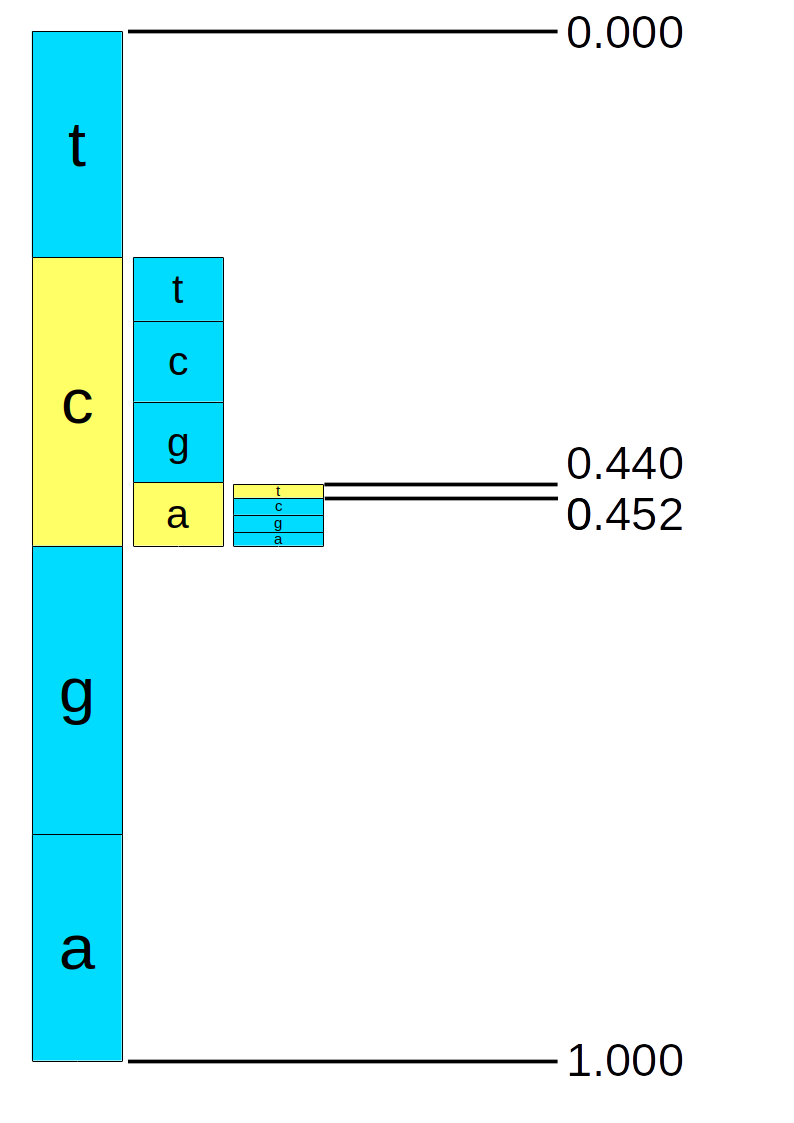
\includegraphics[height=250pt, keepaspectratio=true]{img/range_code.png}

Decoding is simply the reverse of this.  In the above picture we can see that 0.45 would read off `c', `a' and `t' by repeatedly comparing the symbol ranges to the current range and using those to identify the symbol and produce a new range.

\begin{threeparttable}[t]
\begin{tabular}{rrrr}
\hline
\textbf{Range low} & \textbf{Range high} & \textbf{Fraction into range} & \textbf{Symbol}\\
\hline
0.000 & 1.000 & 0.450 & c\\
0.200 & 0.500 & 0.833\tnote{\textbf{a}} & a\\
0.440\tnote{\textbf{b}} & 0.500 & 0.167 & t\\
\hline
\end{tabular}
\begin{tablenotes}
\item{\textbf{a.}} 0.45 into range 0.2 to 0.5: $(0.45-0.2)/(0.5-0.2) = 0.833$.
This falls within the 0.8 to 1.0 symbol range for `a'.
\item{\textbf{b.}} `a' symbol range 0.8 to 1.0 applied to range 0.2 to 0.5:  $0.2+0.8\times(0.5-0.2) = 0.44$ and $0.2+1.0\times(0.5-0.2) = 0.5$.
\end{tablenotes}
\end{threeparttable}

Note: The above example not how the actual implementation works\footnote{This implementation was designed by Eugene Shelwein, based on Michael Schindler's earlier work.}.
For efficiency, we use integer values having a starting range of 0 to $2^{32}-1$.
We write out the top 8-bits of the range when low and high become the same value.
Special care needs to be taken to handle small values are are numerically close but stradding a top byte value, such as 0x37ffba20 to 0x38000034.
The decoder does not need to do anything special here, but the encoder must track the number of 0xff or 0x00 values to emit in order to avoid needing arbitrary precision integers.

Pseudocode for the range codec decoding follows.
This implementation uses code (next few bytes in the current bit-stream) and range instead of low and high, both 32-bit unsigned integers.
This specification focuses on decoding, but given the additional complexity of the precision overflows in encoder we describe this implementation too.

\textsc{RangeDecodeCreate} initialises the range coder, reading the first bytes of the compressed data stream.

\begin{algorithmic}[1]
\Function{RangeDecodeCreate}{}
  \settowidth{\maxwidth}{range\ }
  %\State \algalign{low}{\gets} $0$\Comment{32-bit unsigned}
  \State \algalign{range}{\gets} $2^{32}-1$\Comment{Maximum 32-bit unsigned value}
  \State \algalign{code}{\gets} $0$\Comment{32-bit unsigned}
  \For{$i \gets 0$ to $4$}
    \State $code \gets (code \shiftl 8) + $\Call{ReadUint8}{}
  \EndFor
  \State $code \gets code \bitand 2^{32}-1$
  \State \Return this range coder ($range$, $code$)
\EndFunction
\end{algorithmic}

Decoding each symbol is in two parts; getting the current frequency and updating the range.

\begin{algorithmic}[1]
\Function{RangeGetFreq}{$tot\_freq$}
  \State $range \gets range \bdiv tot\_freq$
  \State \Return $code \bdiv range$
\EndFunction
\end{algorithmic}

\begin{algorithmic}[1]
\Procedure{RangeDecode}{$sym\_low, sym\_freq, tot\_freq$}
  \settowidth{\maxwidth}{range\ }
  \State \algalign{code}{\gets} $code - sym\_low \times range$
  \State \algalign{range}{\gets} $range \times sym\_freq$

  \While{$range < 2^{24}$} \Comment{Renormalise}
    \settowidth{\maxwidth}{range\ }
    \State \algalign{range}{\gets} $range \shiftl 8$
    \State \algalign{code}{\gets} $(code\shiftl8) + $\Call{ReadUint8}{}
  \EndWhile
\EndProcedure
\end{algorithmic}

As mentioned above, the encoder is more complex as it cannot shift out the top byte until it has determined the value.
This can take a considerable while if our current low / high (low + range) are very close but span a byte boundary, such as 0x37ffba20 to 0x38000034, where ultimately we will later emit either 0x37 or 0x38.
To handle this case, when the range gets too small but the top bytes still differ, the encoder caches the top byte of low (0x37) and keeps track of how many 0xff or 0x00 values will need to be written out once we finally observe which value the range has shrunk to.

The \textsc{RangeEncode} function is a straight forward reversal of the \textsc{RangeDecode}, with the exception of the special code for shifting the top byte out of the $low$ variable.

\begin{algorithmic}[1]
\Procedure{RangeEncode}{$sym\_low, sym\_freq, tot\_freq$}
  \settowidth{\maxwidth}{old\_low\ }
  \State \algalign{old\_low}{\gets} $low$
  \State \algalign{range}{\gets} $range \bdiv tot\_freq$
  \State \algalign{low}{\gets} $low + sym\_low \times range$
  \State \algalign{range}{\gets} $range \times sym\_freq$

  \Statex
  \If{low < old\_low}
    \State $carry \gets 1$ \Comment{overflow}
  \EndIf
  \While{$range < 2^{24}$} \Comment{Renormalise}
    \settowidth{\maxwidth}{range\ }
    \State \algalign{range}{\gets} $range \shiftl 8$
    \State \Call{RangeShiftLow}{}
  \EndWhile
\EndProcedure
\end{algorithmic}

\textsc{RangeShiftLow} is the main heart of the encoder renormalisation.
It tracks the total number of extra bytes to emit and $carry$ indicates whether they are a string of 0xFF or 0x00 values.

\begin{algorithmic}[1]
\Procedure{RangeShiftLow}{}
  \If{$low < $ 0xff000000 $\logor carry \ne 0$}
    \If{$carry = 0$}
      \State \Call{WriteByte}{$cache$} \Comment{top byte $cache$ plus FFs}
      \While{$FFnum > 0$}
        \State \Call{WriteByte}{0xff}
        \State $FFnum \gets FFnum - 1$
      \EndWhile
    \Else
      \State \Call{WriteByte}{$cache + 1$} \Comment{top byte $cache+1$ plus 00s}
      \While{$FFnum > 0$}
        \State \Call{WriteByte}{0}
        \State $FFnum \gets FFnum - 1$
      \EndWhile
    \EndIf
    \State $cache \gets low \shiftr 24$ \Comment{Copy of top byte ready for next flush}
    \State $carry \gets 0$
  \Else
    \State $FFnum \gets FFnum + 1$
  \EndIf
  \Statex
  \State $low \gets low \shiftl 8$
\EndProcedure
\end{algorithmic}

For completeness, the Encoder initialisation and finish functions are below.

\begin{algorithmic}[1]
\Procedure{RangeEncodeStart}{}
  \settowidth{\maxwidth}{FFnum\ }
  \State \algalign{low}{\gets} $0$
  \State \algalign{range}{\gets} $2^{32}-1$
  \State \algalign{FFnum}{\gets} $0$
  \State \algalign{carry}{\gets} $0$
  \State \algalign{cache}{\gets} $0$
\EndProcedure
\end{algorithmic}

\begin{algorithmic}[1]
\Procedure{RangeEncodeEnd}{}
  \For{$i \gets 0$ to $4$} \Comment{Flush any residual state in $low$}
    \State \Call{RangeShiftLow}{}
  \EndFor
\EndProcedure
\end{algorithmic}


\subsection{Statistical Modelling}

The probabilities passed to the range coder may be fixed for all scenarios (as we had in the ``cat'' example), or they may be adaptive and context aware.
For example the letter `u' occurs around 3\% of time in English text, but if the previous letter was `q' it is close to 100\% and if the previous letter was `u' it is close to 0\%.
Using the previous letter is known as an Order-1 entropy encoder, but the context can be anything.
We can also adaptively adjust our probabilities as we encode or
decode, learning the likelihoods and thus avoiding needing to store
frequency tables in the data stream covering all possible contexts.

To do this we use a statistical model, containing an array of symbols $S$ and their frequencies $F$.
The sum of these frequences must be less than $2^{16}-32$.
When they get too high, they are renormalised by approximately halving the frequencies (ensuring none drop to zero).

Typically an array of models are used where the array index represents the current context.

To encode any symbol the entropy encoder needs to know the frequency of the symbol to encode, the cumulative frequencies of all symbols prior to this symbol, and the total of all frequencies.
For decoding a cumulative frequency is obtained given the frequency total and the appropriate symbol is found matching this frequency.
Symbol frequencies are updated after each encode or decode call and the symbols are kept in order of most-frequent symbol first in order to  reduce the overhead of scanning through the cumulative frequencies.

\textsc{ModelCreate} initialises a model by setting every symbol to have a frequency of 1.
(At no point do we permit any symbol to have zero frequency.)

\begin{algorithmic}[1]
\Function{ModelCreate}{$num\_sym$}
  \State $total\_freq \gets num\_sym$
  \State $max\_sym \gets num\_sym-1$
  \For{$i \gets 0$ to $max\_sym$}
    \State $S_i \gets i$
    \State $F_i \gets 1$
  \EndFor
  \State \Return this model ($total\_freq$, $max\_sym$, $S$, $F$)
\EndFunction
\end{algorithmic}

\textsc{ModelDecode} is called once for each decoded symbol.
It returns the next symbol and updates the model frequencies automatically.

\begin{algorithmic}[1]
\Function{ModelDecode}{rc}
  \State $freq \gets$ $rc.$\Call{RangeGetFrequency}{$total\_freq$}
  \State $x \gets 0$
  \State $acc \gets 0$
  \While{$acc + F_x \le freq$}
    \State $acc \gets acc + F_x$
    \State $x \gets x+1$
  \EndWhile
  \State $rc.$\Call{RangeDecode}{$acc,\ F_x,\ total\_freq$}
  \State $F_x \gets F_x + 16$ \Comment{Update model frequencies}
  \State $total\_freq \gets total\_freq + 16$
  \If{$total\_freq > 2^{16}-17$}
    \State \Call{ModelRenormalise}{}
  \EndIf
  \State $sym \gets S_x$
  \If{$x > 0 \logand F_x > F_{x-1}$}
    \State \Call{Swap}{$F_x$, $F_{x-1}$}
    \State \Call{Swap}{$S_x$, $S_{x-1}$}
  \EndIf
  \State \Return $sym$
\EndFunction
\end{algorithmic}

\textsc{ModelRenormalise} is called whenever the total frequencies get too high.
The frequencies are halved, taking sure to avoid any zero frequencies being created.

\begin{algorithmic}[1]
\Procedure{ModelRenormalise}{}
  \State $total\_freq \gets 0$
  \For{$i \gets 0$ to $max\_sym$}
    \State $F_i \gets F_i - (F_i \bdiv 2)$
    \State $total\_freq \gets total\_freq + F_i$
  \EndFor
\EndProcedure
\end{algorithmic}

\subsection{Order-0 and Order-1 Encoding}

We can combine the model defined above and the range coder to provide a simple function to perform Order-0 entropy decoder.

\begin{algorithmic}[1]
\Function{DecodeOrder0}{$len$}
  \State $max\_sym \gets $\Call{ReadUint8}{}
  \If{$max\_sym = 0$}
    \State $max\_sym \gets 256$
  \EndIf
  \State $model\_lit \gets $\Call{ModelCreate}{$max\_sym$}
  \Statex
  \State $rc \gets $\Call{RangeDecodeCreate}{}
  \For{$i \gets 0$ to $len-1$}
    \State $out_i \gets model\_lit.$\Call{ModelDecode}{$rc$}
  \EndFor
  \State \Return $out$
\EndFunction
\end{algorithmic}

The Order-1 variant simply uses an array of models and selects the appropriate model based on the previous value encoded or decoded.
This array index is our ``context''.

\begin{algorithmic}[1]
\Function{DecodeOrder1}{$len$}
  \State $max\_sym \gets $\Call{ReadUint8}{}
  \If{$max\_sym = 0$}
    \State $max\_sym \gets 256$
  \EndIf
  \For{$i \gets 0$ to $max\_sym-1$}
    \State $model\_lit_i \gets $\Call{ModelCreate}{$max\_sym$}
  \EndFor
  \Statex
  \State $rc \gets $\Call{RangeDecodeCreate}{}
  \State $last \gets 0$
  \For{$i \gets 0$ to $len-1$}
    \State $out_i \gets model\_lit_{last}.$\Call{ModelDecode}{$rc$}
    \State $last \gets out_i$
  \EndFor
  \State \Return $out$
\EndFunction
\end{algorithmic}

\subsection{RLE with Order-0 and Order-1 Encoding}

The \textsc{DecodeOrder0} and \textsc{DecodeOrder1} codecs can be expanded to include a count of how many runs of each symbol should be decoded.
Both order 0 and order 1 variants are possible.

After the symbol is decoded, the run length must be decoded to
indicate how many \emph{extra} copies of this symbol occur.  Long runs
are broken into a series of lengths of no more than 3.  If length 3
is decoded it indicates we must decode an additional length and add to
the current one.  The context used for the run length model is the
symbol itself for the initial run, 256 for the first continuation run
(if $\ge 4$) and 257 for any further continuation runs.  Thus encoding
10 `A' characters would first store symbol `A' followed by run length
3 (with context `A'), length 3 (context 256), length 3 (context
257), and length 1 (context 258).

For example, if we have the string ``RRRRUNN'' we will decode
symbol `R' run 3, symbol `U' run 0, symbol `N' run 1.

\begin{algorithmic}[1]
\Function{DecodeRLE0}{$len$}
  \State $max\_sym \gets $\Call{ReadUint8}{}
  \If{$max\_sym = 0$}
    \State $max\_sym \gets 256$
  \EndIf
  \State $model\_lit \gets $\Call{ModelCreate}{$max\_sym$}

  \For{$i \gets 0$ to $257$}
    \State $model\_run_i \gets $\Call{ModelCreate}{$4$}
  \EndFor
  \Statex
  \State $rc \gets $\Call{RangeDecodeCreate}{}
  \State $i \gets 0$
  \While{$i < len$}
    \State $out_i \gets model\_lit.$\Call{ModelDecode}{$rc$}
    \State $part \gets model\_run_{out_i}.$\Call{ModelDecode}{$rc$}
    \State $run \gets part$
    \State $rctx \gets 256$
    \While{$part = 3$}
      \State $part \gets model\_run_{rctx}.$\Call{ModelDecode}{$rc$}
      \State $rctx \gets 257$
      \State $run \gets run + part$
    \EndWhile
    \For{$j \gets 1$ to $run$}
      \State $out_{i+j} \gets out_i$
    \EndFor
    \State $i \gets run+1$
  \EndWhile
  \State \Return $out$
\EndFunction
\end{algorithmic}

The order-1 run length variant is identical to order-0 except the
previous symbol is used as the context for the next literal.  The
context for the run length does not change.

\begin{algorithmic}[1]
\Function{DecodeRLE1}{$len$}
  \State $max\_sym \gets $\Call{ReadUint8}{}
  \If{$max\_sym = 0$}
    \State $max\_sym \gets 256$
  \EndIf
  \For{$i \gets 0$ to $max\_sym-1$}
    \State $model\_lit_i \gets $\Call{ModelCreate}{$max\_sym$}
  \EndFor
  \For{$i \gets 0$ to $257$}
    \State $model\_run_i \gets $\Call{ModelCreate}{$4$}
  \EndFor
  \Statex
  \State $rc \gets $\Call{RangeDecodeCreate}{}
  \State $last \gets 0$
  \State $i \gets 0$
  \While{$i < len$}
    \State $out_i \gets model\_lit_{last}.$\Call{ModelDecode}{$rc$}
    \State $last \gets out_i$
    \State $part \gets model\_run_{last}.$\Call{ModelDecode}{$rc$}
    \State $run \gets part$
    \State $rctx \gets 256$
    \While{$part = 3$}
      \State $part \gets model\_run_{rctx}.$\Call{ModelDecode}{$rc$}
      \State $rctx \gets 257$
      \State $run \gets run + part$
    \EndWhile
    \For{$j \gets 1$ to $run$}
      \State $out_{i+j} \gets last$
    \EndFor
    \State $i \gets run+1$
  \EndWhile
  \State \Return $out$
\EndFunction
\end{algorithmic}

%\subsection{General Purpose Entropy Encoder}

We wrap up the Order-0 and 1 entropy encoder, both with and without run length encoding, into a data stream that specifies the type of encoded data and also permits a number of additional transformations to be applied.
These transformations support bit packing (for example a data block with only 4 distinct values can be packed with 4 values per byte), no-op for tiny data blocks where entropy encoding would grow the data and N-way interleaving of the 8-bit components of a 32-bit value.

\begin{table}[h]
\centering
\begin{tabular}{|r|r|r|r|p{9cm}|l|}
\hline
\multicolumn{2}{|r|}{\textbf{Bits} } & \textbf{Type}  & \textbf{Name} & \multicolumn{2}{p{9cm}|}{\textbf{Description}} \\
\hline
\multicolumn{2}{|r|}{8} & uint8 & $flag$ & \multicolumn{2}{p{9cm}|}{Data format bit field}\\
\cline{1-6}

\multicolumn{6}{|l|}{}\\[-0.3em]
\multicolumn{6}{|l|}{\textit{Unless \textsc{NoSize} flag is set:} } \\
\cline{2-5}
& ? & uint7 & ulen & Uncompressed length & \\
\cline{2-5}

\multicolumn{6}{|l|}{}\\[-0.3em]
\multicolumn{6}{|l|}{\textit{If \textsc{Stripe} flag is set:} } \\
\cline{2-5}
& ? & uint8 & N & Number of sub-streams & \\
& ? & uint7[] & clen[] & N copies of compressed sub-block length & \\
& ? & uint8[] & cdata[] & N copies of Compressed data sub-block (recurse) & \\
\cline{2-5}

\multicolumn{6}{|l|}{}\\[-0.7em]
\multicolumn{6}{|l|}{\textit{If \textsc{Cat} flag is set (and \textsc{Stripe} flag is unset):} } \\
\cline{2-5}
& ? & uint8[] & udata & Uncompressed data stream & \\
\cline{2-5}

\multicolumn{6}{|l|}{}\\[-0.7em]
\multicolumn{6}{|l|}{\textit{If \textsc{Pack} flag is set (and neither \textsc{Stripe} or \textsc{Cat} flags are set):} } \\
\cline{2-5}
& ? & uint8[] & pack\_meta & Pack lookup table & \\
\cline{2-5}

\multicolumn{6}{|l|}{}\\[-0.7em]
\multicolumn{6}{|l|}{\textit{If neither \textsc{Stripe} or \textsc{Cat} flags are set:} } \\
\cline{2-5}
& ? & uint8[] & cdata & Entropy encoded data stream (see \textsc{Order} / \textsc{RLE} / \textsc{Ext} flags) & \\
\cline{2-5}
\multicolumn{6}{|l|}{}\\
\hline
\end{tabular}
\end{table}

The first byte of our generalised data stream is a bit-flag detailing the type of transformations and entropy encoders to be combined, followed by optional meta-data, followed by the actual compressed data stream.
The bit-flags are defined below, but note not all combinations are permitted.

\begin{threeparttable}[t]
\begin{tabular}{llll}
\hline
\textbf{Bit AND value} & \textbf{Code} & \textbf{Description} \\
\hline
1 & \textsc{Order}\tnote{\textbf{a}} & Order-0 or Order-1 entropy coding. \\
2 & reserved & Reserved (for possible order-2/3)\\
4 & \textsc{Ext} & ``External'' compression via bzip2\\
8 & \textsc{Stripe}\tnote{\textbf{b}} & N-way interleaving of byte streams.\\
16 & \textsc{NoSize} & original size is not recorded (used by \textsc{Stripe})\\
32 & \textsc{Cat}\tnote{\textbf{b}} & Data is uncompressed\\
64 & \textsc{RLE}\tnote{\textbf{a}} & Run length encoding, with runs and literals encoded separately\\
128 & \textsc{Pack} & Pack 2, 4, 8 or infinite symbols per byte.\\
\hline
\end{tabular}
\begin{tablenotes}
\item{\textbf{a.}} Has no effect when \textsc{Ext} flag is set.
\item{\textbf{b.}} Not to be used in conjunction with other flags
  except \textsc{Pack} and \textsc{NoSize}.
\end{tablenotes}
\end{threeparttable}

Of these \textsc{Stripe} is the most complex.
As with the rANS4x16 encoder, the data is rearranged such that every
$N^{th}$ byte is adjacent in a single block producing N distinct sub-blocks.
Each of the N streams is then itself compressed using this compression format.

For example an input block of small unsigned 32-bit little-endian numbers may use RLE for the first three streams as they are mostly zero, and a non-RLE Order-0 entropy encoder of the last stream.
Normally our data format will include the decoded size, but with \textsc{Stripe} we can omit this from the internal compressed streams as we know their size will be a computable fraction of the combined data.

The data layout differs for each of these bit types, as described below in the \textsc{ArithDecode} function.
Some of these can be used in combination, so the order needs to be observed.
The Pack format has additional meta data.
This is decoded first, before entropy decoding and finally expanding thespecified pack transformation after decompression.
For example value 193 is indicates a byte stream should be decoded with an RLE aware order-1 entropy encoder and then unpacked.

\begin{algorithmic}[1]
\Function{ArithDecode}{$len$}
  \State $flags \gets $\Call{ReadUint8}{}
  \If{$flags \bitand$ \textsc{NoSize} $\ne 0$}
    \State $len \gets$\Call{ReadUint7}{}
  \EndIf
  \If{$flags \bitand$ \textsc{Stripe}}
    \State $data \gets $\Call{DecodeSTRIPE}{$len$}
    \State \Return $data$
  \EndIf{}
  \If{$flags \bitand$ \textsc{Pack}}
    \State $pack\_len \gets len$
    \State $(P,\ nsym,\ len) \gets $\Call{DecodePackMeta}{}
  \EndIf
  \Statex \Comment{Entropy Decoding}
  \If{$flags \bitand$ \textsc{Cat}}
    \State $data \gets $\Call{ReadData}{$len$}
  \ElsIf{$flags \bitand$ \textsc{Ext}}
    \State $data \gets $\Call{DecodeEXT}{$len$}
  \ElsIf{$flags \bitand$ \textsc{RLE}}
    \If{$flags \bitand$ \textsc{Order}}
      \State $data \gets $\Call{DecodeRLE1}{$len$}
    \Else
      \State $data \gets $\Call{DecodeRLE0}{$len$}
    \EndIf
  \Else
    \If{$flags \bitand$ \textsc{Order}}
      \State $data \gets $\Call{DecodeOrder1}{$len$}
    \Else
      \State $data \gets $\Call{DecodeOrder0}{$len$}
    \EndIf
  \EndIf
  \Statex \Comment{Apply data transformations}
  \If{$flags \bitand$ \textsc{Pack}}
    \State $data \gets $\Call{DecodePack}{$data$, $P$, $nsym$, $pack\_len$}
  \EndIf
  \State \Return $data$
  \EndFunction
\end{algorithmic}

The specifics of each sub-format are described below, in the order (minus meta-data specific shuffling) they are applied.

\begin{itemize}
\item{\textbf{\textsc{Stripe}}:}
The byte stream consists of a 7-bit encoded uncompressed length and a
byte holding the number of substreams $N$, and their 7-bit encoded
compressed data streams lengths.  This is then followed by the
substreams themselves, each of which is a valid $cdata$ stream as
defined above, hence this offers a recursive mechanism as each
substream has its own format byte.

The total uncompressed byte stream is then an interleaving of one byte
in turn from each of the N substreams (in order of 1st to Nth).  Thus
an array of 32-bit unsigned integers could be unpacked using
\textsc{Stripe} to compress each of the 4 8-bit components together with
their own algorithm.

\begin{algorithmic}[1]
\Function{RansDecodeStripe}{$len$}
  \State $N \gets $\Call{ReadUint8}{}
  \For{$j \gets 0$ to $N$} \Comment{Fetch N compressed lengths}
    \State $clen_j \gets $\Call{ReadUint7}{}
  \EndFor
  \Statex
  \For{$j \gets 0$ to $N$} \Comment{Decode N streams}
    \State $ulen_j \gets (len \bdiv N) + ((len \bmod N) > j)$
\Comment{$(x > y)$ expression being 1 if true, 0 if false}
    \State $T_j \gets $\Call{ArithDecode}{$ulen_j$}
  \EndFor
  \Statex
%  \For{$i \gets 0$ to $len - 1$} \Comment{Interleave}
%    \State $out_i \gets T_{(i \bmod N),\ (i \bdiv N)}$
%  \EndFor
  \For{$j \gets 0$ to $N - 1$} \Comment{Interleave}
    \For{$i \gets 0$ to $ulen_j - 1$}
      \State $out_{i \times N + j} \gets T_{j,i}$
    \EndFor
  \EndFor
  \State \Return $out$
\EndFunction
\end{algorithmic}

\item{\textbf{\textsc{NoSize}}:}
Do not store the size of the uncompressed data stream.
This information is not required when the data stream is one of the four sub-streams in the \textsc{Stripe} format.

\item{\textbf{\textsc{Cat}}:}
If present, all other bit flags should be nul, with the possible
exception of \textsc{NoSize} or \textsc{Pack}.

The uncompressed data stream is the same as the compressed stream.
This is useful for very short data where the overheads of compressing are too high.

\item{\textbf{\textsc{Order}}:}
Bit field defining order-0 (unset) or order-1 (set) entropy encoding, as described above by the \textsc{DecodeOrder0} and \textsc{DecodeOrder1} functions.

\item{\textbf{\textsc{RLE}}:}
Bit field defining whether the Order-0 and Order-1 encoding should also use a run-length.
When set, the \textsc{DecodeRLE0} and \textsc{DecodeRLE1} functions will be used instead of \textsc{DecodeOrder0} and \textsc{DecodeOrder1}.

\item{\textbf{\textsc{Ext}}:}
Instead of using the adaptive arithmetic coder for decompression (with or without RLE), this uses an compression codec defined in an ``external'' library.
Currently the only supported such codec is Bzip2.
In future more may be added, so the magic number \emph{must} be validated to check the codec being used.

Given bzip2 is already supported elsewhere in CRAM, the purpose of adding it here is to permit bzip2 compression after \textsc{Pack} and \textsc{Stripe} transformations.
This may be tidied up in later CRAM releases to clarify the separation between compression codecs and data transforms, but that requires more major restructuring so for compatibility with v3.0 these have been placed into this single codec.

\begin{algorithmic}[1]
\Function{DecodeExt}{$len$}
  \If{Bzip2 magic number is present}
    \State \Return \Call{DecodeBzip2}{$len$}
  \Else
    \State Error
  \EndIf
\EndFunction
\end{algorithmic}

\item{\textbf{\textsc{Pack}}:}
Data containing only 1, 2, 4 or 16 distinct values can have multiple
values packed into a single byte (infinite, 8, 4 or 2).  The distinct
symbol values do not need to be adjacent as a mapping table $P$
converts mapped value $x$ to original symbol $P_x$.

The packed format is split into uncompressed meta-data (below) and the
compressed packed data as described in the rANS 4x16 bit-packing section.
The same \textsc{DecodePackMeta} and \textsc{DecodePack} functions are used.

\end{itemize}

\section{Name tokenisation codec}

Sequence names (identifiers) typically follow a structured pattern and compression based on columns within those structures usually leads to smaller sizes.
The sequence name (identifier) tokenisation relies heavily on the General Purpose Entropy Encoder described above.

As an example, take a series of names:

\begin{verbatim}
I17_08765:2:123:61541:01763#9
I17_08765:2:123:1636:08611#9
I17_08765:2:124:45613:16161#9
\end{verbatim}

We may wish to tokenise each of these into 7 tokens, e.g.
``I17\_08765:2:'', ``123'', ``:'', ``61541'', ``:'', ``01763''and
``\#9''. Some of these are multi-byte strings, some single characters,
and some numeric, possibily with a leading zero.  We also observe some
regularly have values that match the previous line (the initial prefix
string, colons, ``\#9'') while others are numerically very close to the
value in the previous line (124 vs 123).

The name tokeniser compares each name against a previous name (which
is not necessarily the one immediately prior) and encodes this name
either as a series of differences to the previous name or marking it
as an exact duplicate.  A maximum of 128 tokens are permitted within
any single read name.

Token IDs (types) are listed below.

\begin{tabular}{lllp{10cm}}
\hline
\textbf{ID} & \textbf{Type} & \textbf{Value} & \textbf{Description}\\
\hline
 0 & TYPE    & Type    & Used to determine the type of token at a given position. \\
\hline
 5 & DUP     & Integer (distance) & The entire name is a duplicate of an earlier one.  Used in position 0 only.\\
 6 & DIFF    & Integer (distance) & The entire name is differs to earlier ones.  Used in position 0 only.\\
\hline
 1 & STRING  & String  & A nul-terminated string of characters \\
 2 & CHAR    & Byte    & A single character \\
 7 & DIGITS  & $0 \le$ Int $< 2^{32}$ & A numerical value, not containing a leadng zero \\
 3 & DIGITS0 & $0 \le$ Int $< 2^{32}$ & A numerical value possibly starting in leading zeros \\
 4 & DZLEN   & Int length & Length of associated DIGITS0 token.\\
 8 & DELTA  & $0 \le$ Int $< 256$   & A numeric value being stored as the difference to the numeric value of this token on the previous name. \\
 9 & DELTA0 & $0 \le$ Int $< 256$ & As DELTA, but for numeric values starting with leading zeros \\
10 & MATCH   & (none) & This token is identical type and value to the same position in the previous name (NB: not permitted for DELTA/DELTA0)\\
11 & NOP & (none) & Does nothing\\
12 & END     & (none) & Marks end of name\\
\hline
\end{tabular}

The tokens and values are stored in a 2D array of byte streams,
$B_{pos,type}$, where pos 0 is reserved for name meta-data (whether it
is a duplicate name) and pos 1 onwards is for the first, second and
later tokens.  $Type$ is one of the token types listed above,
corresponding to the type of data being stored.  Some token types may
also have associated values.  $B_{pos,\texttt{TYPE}}$ ($type$) holds the token
type itself and that is then used to retrieve any associated
value(s) if appropriate from $B_{pos,type}$.  Thus multiple types at the same token
position will have their values encoded in distinct data streams,
e.g. if position 5 is of type either DIGITS or DELTA then data streams
will exist for $B_{5,\texttt{TYPE}}$, $B_{5,\texttt{DIGITS}}$ and $B_{5, \texttt{DELTA}}$.
Decoding per name continues until a token of type END is observed.

More detail on the token types is given below.

\begin{itemize}
\item{\textbf{TYPE}:}
This is the first token fetched at each token position.  It holds the
type of the token at this position, which in turn may then require
retrieval from type-specific data streams at this position.

For position 0, the TYPE field indicates whether this record is an
exact duplicate of a prior read name or has been encoded as a delta to
an earlier one.

\item{\textbf{DUP}, \textbf{DIFF}:}
These types are fetched for position 0, at the start of each new
identifier.  The value is an integer value describing how many reads
before this (with 1 being the immediately previous name) we are
comparing against.  When we refer to ``previous name'' below, we
always mean the one indicated by the DIFF field and not the one
immediately prior to the current name.

The first record will have a DIFF of zero and no delta or match
operations are permitted.

\item{\textbf{STRING}:}
We fetch one byte at a time from the value byte stream, appending to the
name buffer until the byte retrieved is zero.  The zero byte is not
stored in the name buffer.
For purposes of token type MATCH, a match is defined as entirely
matching the string including its length.

\item{\textbf{CHAR}:}
Fetch one single byte from the value byte stream and append to the name buffer.

\item{\textbf{DIGITS}:}
Fetch 4 bytes from the value byte stream and intrepret these as a little
endian unsigned integer.  This is appended to the name buffer as
string of base-10 digits, most significant digit first.  Larger
values may be represented, but will require multiple DIGITS tokens.
Negative values may be encoded by treating the minus sign as a CHAR or
STRING and storing the absolute value.

\item{\textbf{DIGITS0}, \textbf{DZLEN}:}
This fetches the 4 byte value from $B_{pos,DIGITS0}$ and a 1 byte
length from $B_{pos,DZLEN}$.  As per DIGITS, the value is intrepreted as a
little endian unsigned integer.  The length indicates the total
size of the numeric value when displayed in base 10 which must be
greater than $\log_{10}(value)$ with any remaining length indicating
the number of leading zeros.  For example if DIGITS0 value is 123 and
DZLEN length is 5 the string ``00123'' must be appended to the name.

For purposes of the MATCH type, both value and length must match.

\item{\textbf{DELTA}:}
Fetch a 1 byte value and add this to the DIGITS value from the
previous name.
The token in the prior name must be of type DIGITS or DELTA.

MATCH is not supported for this type.

\item{\textbf{DELTA0}:}
As per DELTA, but the 1 byte value retrieved is added to the DIGITS0
value in the previous name.  No DZLEN value is retrieved, with the
length from the previous name being used instead.
The token in the prior name must be of type DIGITS0 or DELTA0.

MATCH is not supported for this type.

\item{\textbf{MATCH}:}
This token matches the token at the same position in the previous
name.  (The previous name is permitted to also have a MATCH token at
this position, in which case it recurses to its previous name.)

MATCH is only valid when the token being matched against is CHAR,
STRING, DIGITS, DIGITS0 or MATCH.  (I.e. matching a numeric delta will not
repeat the delta increment.)

No value is needed for MATCH tokens.

\item{\textbf{NOP}:}
This token type does nothing.
The purpose of this is simply to permit skipping tokens in order to
keep token numbers in sync, such as when processing ``10'' vs ``-10''
with the latter needing an additional ``-'' token.

\item{\textbf{END}:}
Marks the end of the name.  A nul byte is added to the name output
buffer.  No value is needed for END tokens.
\end{itemize}

Decoding needs some simple functions to read successive bytes from our token byte streams, as 8-bit characters or unsigned integers, as 32-bit unsigned integers and nul-terminated strings.  We reuse the \textsc{ReadUint32} and related functions with the byte array specified as input.

\begin{algorithmic}[1]
\Statex
\Statex \textit{(Convert an integer to a string form in base-10 digits, at least $len$ bytes long with leading zeros)}
\Function{LeftPadNumber}{$val,\ len$}
  \State $str \gets val$ \Comment{Implicit language-specific Integer to String conversion}
  \While{\Call{Length}{$str$} < $len$}
    \State $str \gets$ `$0$' $ \concat str$
  \EndWhile
  \State \Return $str$
\EndFunction
\end{algorithmic}

For the main name decoding loop, we use a single dimensional array of
names decoded so far, $N$, and a two dimensional array of their tokens
$T$ (indexed by name number $n$ and token position $t$ within that
name).  We define a function to decode the $n^{th}$ name ($N_n$) using
a previous $m^{th}$ name ($N_m$).  The tokens $T$ are used in
\texttt{MATCH} and \texttt{DELTA} token types to copy data from when
constructing the name.

Now we have the basic primitives for pulling from the $B$ byte
streams, decoding the $n^{th}$ individual name is as
follows\footnote{For simplicity of algorithm description, we take a
  flexible approach as to whether we read/write $T$ in numeric or
  string form.  For example a \texttt{DELTA} token will fetch the
  previous token as a string, interpret it as a numeric value, add to
  it, and then write it back as a string.  Practical implementations
  may wish to separate out T into distinct integer and string
  arrays.}:


\begin{algorithmic}[1]
\Statex
\Statex \textit{(Decodes the $n^{th}$ name, returning $N_n$ and updating globals $N_n$ and $T_n$)}
\Function{DecodeSingleName}{$n$}
  \State $type \gets$ \Call{ReadUint8}{$B_{0,\textit{TYPE}}$}
  \State $dist \gets$ \Call{ReadUint32}{$B_{0,type}$}
  \State $m \gets n-dist$
  \If{$type = $ \texttt{DUP}}
    \State $N_n \gets N_m$
    \State $T_n \gets T_m$ \Comment{Copy for all $T_{n,*}$}
    \State \Return $N_n$
  \EndIf
  \Statex
  \State $t \gets 1$ \Comment{Token number $t$}
  \Repeat
    \State $type \gets$ \Call{ReadUint8}{$B_{t,\texttt{TYPE}}$}
    \If{$type = $ \texttt{CHAR}}
      \State $T_{n,t} \gets$ \Call{ReadChar}{$B_{t,\texttt{CHAR}}$}
    \ElsIf{$type = $ \texttt{STRING}}
      \State $T_{n,t} \gets$ \Call{ReadString}{$B_{t,\texttt{STRING}}$}
    \ElsIf{$type = $ \texttt{DIGITS}}
      \State $T_{n,t} \gets$ \Call{ReadUint32}{$B_{t,\texttt{DIGITS}}$}
    \ElsIf{$type = $ \texttt{DIGITS0}}
      \State $d \gets$ \Call{ReadUnt32}{$B_{t,\texttt{DIGITS0}}$}
      \State $l \gets$ \Call{ReadUint8}{$B_{t,\texttt{DZLEN}}$}
      \State $T_{n,t} \gets$ \Call{LeftPadNumber}{$d,\ l$}
    \ElsIf{$type = $ \texttt{DELTA}}
      \State $T_{n,t} \gets T_{m,t} + $ \Call{ReadUint8}{$B_{t,\texttt{DELTA}}$}
    \ElsIf{$type = $ \texttt{DELTA0}}
      \State $d \gets T_{m,t} + $ \Call{ReadUint8}{$B_{t,\texttt{DELTA0}}$}
      \State $l \gets$ \Call{Length}{$T_{m,t}$} \Comment{String length including leading zeros}
      \State $T_{n,t} \gets$ \Call{LeftPadNumber}{$d,\ l$}
    \ElsIf{$type = $ \texttt{MATCH}}
      \State $T_{n,t} \gets T_{m,t}$
    \Else
      \State $T_{n,t} \gets$\ `'
    \EndIf
    \State $N_n \gets N_n \concat T_{n,t}$
    \State $t \gets t+1$
  \Until{$type = $ \texttt{END}}
  \State \Return $N_n$
\EndFunction
\end{algorithmic}

Given a complex name with both position and type specific values, this
can lead to many separate data streams.  The name tokeniser codec is
a format within a format, as the multiple byte streams $B_{pos,type}$
are serialised into a single byte stream.

The serialised data stream starts with two unsigned little endiand 32-bit
integers holding the total size of uncompressed name buffer and the
number of read names.  This is followed the array elements
themselves.

Token types, $ttype$ holds one of the token ID values listed above
in the list above, plus special values to indicate certain additional
flags.  Bit 6 (64) set indicates that this entire token data stream is a
duplicate of one earlier.  Bit 7 (128) set indicates the token
is the first token at a new position.  This way we only need to store
token types and not token positions.

The total size of the serialised stream needs to be already known, in
order to determine when the token types finish.

\begin{tabular}{|r|r|r|l|l|p{10cm}|}
\hline
\multicolumn{3}{|r|}{\textbf{Bytes}} & \textbf{Type} & \textbf{Name} & \textbf{Description}\\
\hline
\multicolumn{3}{|r|}{4} & uint32 & $uncomp\_length$ & Length of uncompressed name buffer\\
\multicolumn{3}{|r|}{4} & uint32 & $num\_reads$ & Number of read names\\
\multicolumn{3}{|r|}{1} & uint8  & $use\_arith$ & Whether compression is arithmetic (1) or rANS4x16 (0)\\
\hline
\multicolumn{6}{|l|}{\quad\textit{For each token data stream}}\\
\cline{2-6}
& \multicolumn{2}{r|}{1} & uint8 & $ttype$ & Token type code plus flags (64=duplicate, 128=next token position).\\
\cline{2-6}
& \multicolumn{5}{l|}{\textit{If ttype AND 64 (duplicate)}}\\
\cline{3-6}
& & 1 & uint8 & $dup\_pos$  & Duplicate from this token position\\
& & 1 & uint8 & $dup\_type$ & Duplicate from this token type ID\\
\cline{3-6}
& \multicolumn{5}{l|}{\textit{else if not duplicate}}\\
\cline{3-6}
& & ? & i7 & $clen$ & compressed length (7-bit encoding)\\
& & $clen$ & $cdata$ & stream & compressed data stream\\
\hline
\end{tabular}

A few tricks are used to remove some byte streams.  In addition to the explicit marking of duplicate bytes streams, if a byte stream of token types is entirely MATCH apart from the very first value it is discarded.  It is possible to regenerate this during decode by observing the other byte streams.  For example if we have a byte stream $B_{5,DIGITS}$ but no $B_{5,TYPE}$ then we assume the contents of $B_{5,TYPE}$ consist of one DIGITS type followed by as many MATCH types as are needed.

The $cdata$ stream itself is as described in the General Purpose Entropy Encoder section above, with the \textsc{ArithDecode} function.

\begin{algorithmic}[1]
\Statex
\Statex \textit{(Decodes and uncompressed the serialised token byte streams)}
\Function{DecodeTokenByteStreams}{$use\_arith$}
  \State $sz \gets 0$
  \State $t \gets -1$
  \Repeat
    \State $ttype \gets$ \Call{ReadUint8}{}
    \State $tok\_new \gets ttype \bitand 128$
    \State $tok\_dup \gets ttype \bitand 64$
    \State $type \gets ttype \bitand 63$
    \If{$tok\_new \ne 0$}
      \State $t \gets t+1$
      \If{$type \ne \texttt{TYPE}$}
        \State $B_{t,\texttt{TYPE}} \gets (type, \texttt{TOK\_MATCH}, \texttt{TOK\_MATCH}, ...)$\Comment{for $nnames-1$ times}
      \EndIf
    \EndIf
    \Statex
    \If{$tok\_dup \ne 0$}
       \State $dup\_pos \gets$ \Call{ReadUint8}{}
       \State $dup\_type \gets$ \Call{ReadUint8}{}
       \State $B_{t,type} \gets B_{dup\_pos,dup\_type}$
    \Else
      \State $clen \gets$ \Call{ReadUint7}{}
      \State $data \gets$ \Call{ReadData}{$clen$}
      \If{$use\_arith$}
        \State $B_{t,type} \gets$ \Call{ArithDecode}{}
      \Else
        \State $B_{t,type} \gets$ \Call{RansDecode4x16}{}
      \EndIf
    \EndIf
  \Until{\Call{EOF}{}}
  \State \Return $B$
\EndFunction
\end{algorithmic}

\begin{algorithmic}[1]
\Statex
\Statex \textit{(Decodes the $n^{th}$ name, returning $N_n$ and updating $N_n$ and $T_n$)}
\Function{DecodeNames}{}
  \State $ulen \gets$ \Call{ReadUint32}{}
  \State $nnames \gets$ \Call{ReadUint32}{}
  \State $use\_arith \gets$ \Call{ReadUint8}{}
  \State $B \gets$ \Call{DecodeTokenByteStreams}{$use\_arith$}

  \For{$n \gets 0$ to $nnames-1$}
    \State $N_n \gets$ \Call{DecodeSingleName}{$n$}
  \EndFor
  \State \Return $N$
\EndFunction
\end{algorithmic}


\section{FQZComp quality codec}

% Ideas to explore and TODO list:
%
% 1. Move param do_rev to global part.  It's all or nothing
%
% 2. Delta updates immediately on base 0 to base 1.  Maybe delay
%    initialisation so prevq is 1st base qual.
%
% 3. ReadArray pseudocode needs fixing.
%
% 4. Add param sel_offset to subtract from decoded sel.
%    Eg if we have 2 params and max_sel 3 (0..3) then we may want
%    sel 0/1 for 1st param and sel 0/1 (sel_offset 2) for 2nd?
%
% 5. Add len_bytes to param so we don't need Model_len[4] always.
%
% 6. Permit do_term and term_sym to put in newlines (or whatever)
%    after each record. (See 7 below for example)
%
% 7. Add dmap to apply to quals before doing the prevq != q check.
%    Reason is maybe we're not compressing qualities!  Eg SA:Z: tag
%    may be best using dmap , = 1 and everything else = 0.  Then
%    ``chr4,100,5,blah''; becomes delta 000012223456666.  dtab to
%    divide by 2 then allows it to track token number.
%    Each semi-colon separated text is a new record (qlen) and they're
%    joined together with term_sym (6. above).
%
% 8. Consider adding selector as context for model len, rev and dup.
%    This is important on mixed data sets.  Do we want full sel, or
%    quantised stab[sel]?

The FQZComp quality codec uses an adaptive statistical model to
predict the next quality value in a given context (comprised of
previous quality values, position along this sequence, whether the
sequence is the second in a pair, and a running total of number of
times the quality has changed in this sequence).

For each quality value, the models produce probabilities for all
possible next quality values, which are passed into an arithmetic
entropy encoder to encode or decode the actual next quality value.
The models are then updated based on the actual next quality in order
to learn the statistical properties of the quality data stream.  This
step wise update process is identical for both encoding and decoding.

The algorithm is a generalisation on the original fqzcomp program,
described in \textit{Compression of FASTQ and SAM Format Sequencing
  Data} by Bonfield JK, Mahoney MV (2013). PLoS ONE 8(3):
e59190. \url{https://doi.org/10.1371/journal.pone.0059190}

\subsection{FQZComp Models}

The FQZComp process utilises knowledge of the read lengths, complement
(qualities reversed) status, and a generic parameter selector, but in
order to maintain a strict separation between CRAM data series this
knowledge is stored (duplicated) within the quality data stream
itself.  Note the complement model is only needed in CRAM 3.1 as CRAM
4 natively stores the quality in the original orientation already.
Both reversed and duplication models have no context and are boolean
values.

The parameter selector model also has no context associated with it
and encodes $max\_sel$ distrinct values.  The selector value may be
quantised further using $stab$ to reduce the selector to fewer
sets of parameters.  This is useful if we wish to use the selector
bits directly in the context using the same parameters.  The selector
is arbitrary and may be used for distinguishing READ1 from READ2, as
a precalculated ``delta'' instead of the running total, distinguishing
perfect alignments from imperfect ones, or any other factor that is
shown to improve quality predictability and increase compression
ratio (average quality, number of mismatches, tile, swathe, proximity
to tile edge, etc).

The quality model has a 16-bit context used to address an array of
$2^{16}$ models, each model permitting $max\_sym$ distinct quality
values.  The context used is defined by the FQZcomp parameters, of
which there may be multiple sets, selected using the selector model.
There are 4 read length models each having $max\_sym$ of 256.  Each
model is used for the 4 successive bytes in a 32-bit length value.

\begin{center}
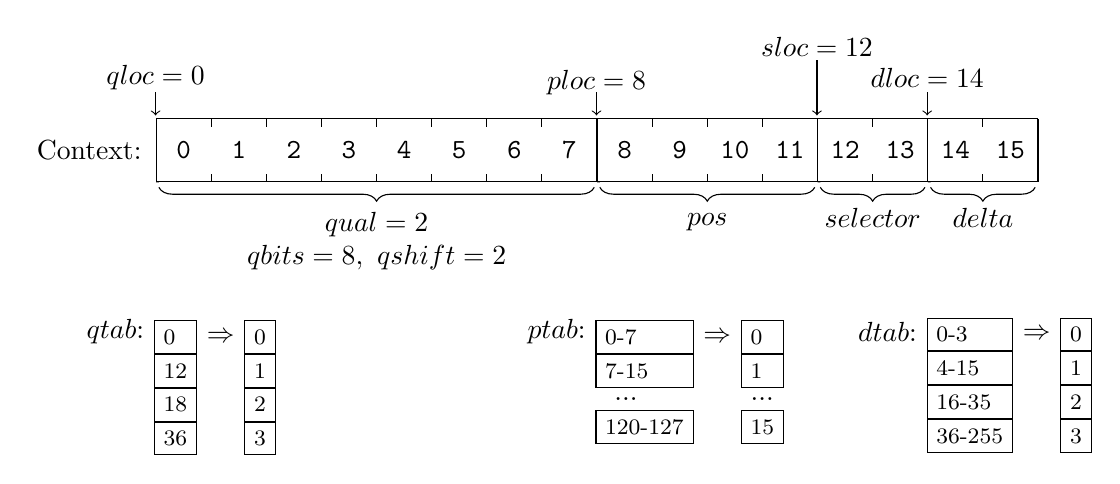
\begin{tikzpicture}[
  boxed/.style={rectangle, draw=black, text width=1cm},
  boxed1/.style={rectangle, draw=black},
  boxed2/.style={rectangle, draw=black, text width=.3cm},
  boxed3/.style={rectangle, draw=black, text width=0.85cm},
]
\newcommand{\x}{0.7cm}
\node at (-0.5, 0) {Context:};
\draw[-] (0*\x+.5*\x,-0.4) -- (0*\x+.5*\x,+0.4);
\foreach \w/\i [count=\n] in {
  3/0, 3/1, 3/2, 3/3, 3/4, 3/5, 3/6, 0/7,   % qual
  3/8, 3/9, 3/10, 0/11,                     % pos
  3/12, 0/13,                               % selector
  3/14, 0/15} {                             % delta
    \draw[-] (\n*\x+.5*\x,-0.4)  -- (\n*\x+.5*\x,-\w/10);
    \draw[-] (\n*\x+.5*\x,\w/10) -- (\n*\x+.5*\x, 0.4);
    \draw[-] (\n*\x-.5*\x,-0.4)  -- (\n*\x+.5*\x,-0.4);
    \draw[-] (\n*\x-.5*\x, 0.4)  -- (\n*\x+.5*\x, 0.4);
    \node(N\n)[minimum height=1cm,minimum width=\x,xshift=\n*\x,font=\ttfamily](N\n){\i};
}
\draw[<-] ([yshift=1pt]N1.north west)+(0,-0.1cm) -- +(0,0.2cm)
    node[yshift=5pt]{$qloc=0$};
\draw[<-] ([yshift=1pt]N9.north west)+(0,-0.1cm) -- +(0,0.2cm)
    node[yshift=3.5pt]{$ploc=8$};
\draw[<-] ([yshift=1pt]N13.north west)+(0,-0.1cm) -- +(0,0.6cm)
    node[yshift=5pt]{$sloc=12$};
\draw[<-] ([yshift=1pt]N15.north west)+(0,-0.1cm) -- +(0,0.2cm)
    node[yshift=5pt]{$dloc=14$};
\draw[decoration={brace,mirror,amplitude=5pt,raise=2pt, post=moveto, pre length=1pt, post length=1pt},decorate]
  (0.5*\x,-0.4) -- node[below=6pt] {\begin{tabular}{c}$qual \shiftl= 2$\\$qbits=8,\ qshift=2$\end{tabular}} +(8*\x,0);
\draw[decoration={brace,mirror,amplitude=5pt,raise=2pt, post=moveto, pre length=1pt, post length=1pt},decorate]
  (8.5*\x,-0.4) -- node[below=8pt] {$pos$} +(4*\x,0);
\draw[decoration={brace,mirror,amplitude=5pt,raise=2pt, post=moveto, pre length=1pt, post length=1pt},decorate]
  (12.5*\x,-0.4) -- node[below=6pt] {$selector$} +(2*\x,0);
\draw[decoration={brace,mirror,amplitude=5pt,raise=2pt, post=moveto, pre length=1pt, post length=1pt},decorate]
  (14.5*\x,-0.4) -- node[below=6pt] {$delta$} +(2*\x,0);

\node[right] (Q) at ([yshift=-1.8cm,xshift=-1cm]N1.south west) {$qtab$:};
\node[above right,boxed2] (Q0) at (Q.south east)  {\footnotesize{0}};
\node[below right,boxed2] (Q1) at (Q0.south west) {\footnotesize{12}};
\node[below right,boxed2] (Q2) at (Q1.south west) {\footnotesize{18}};
\node[below right,boxed2] (Q3) at (Q2.south west) {\footnotesize{36}};

\node[right] (Qeq) at (Q0.east) {$\Rightarrow$};
\node[      right,boxed1] (q0) at (Qeq.east) {\footnotesize{0}};
\node[below right,boxed1] (q1) at (q0.south west) {\footnotesize{1}};
\node[below right,boxed1] (q2) at (q1.south west) {\footnotesize{2}};
\node[below right,boxed1] (q3) at (q2.south west) {\footnotesize{3}};

%\node[right] (P) at ([xshift=3cm]Q.east) {$ptab$:};
\node[right] (P) at ([yshift=-1.8cm,xshift=-1cm]N9.south west) {$ptab$:};
\node[above right,boxed] (P0)   at (P.south east)  {\footnotesize{0-7}};
\node[below right,boxed] (P8)   at (P0.south west) {\footnotesize{7-15}};
\node[below right]       (P16)  at (P8.south west) {\ ...};
\node[below right,boxed] (P124) at (P16.south west) {\footnotesize{120-127}};

\node[right] (Peq) at (P0.east) {$\Rightarrow$};
\node[      right,boxed2] (p0)   at (Peq.east) {\footnotesize{0}};
\node[below right,boxed2] (p8)   at (p0.south west) {\footnotesize{1}};
\node[below right       ] (p16)  at (p8.south west) {...};
\node[below right,boxed2] (p124) at (p16.south west) {\footnotesize{15}};

%\node[right] (D) at ([xshift=4cm]P.east) {$dtab$:};
\node[right] (D) at ([yshift=-1.8cm,xshift=-1cm]N15.south west) {$dtab$:};
\node[above right,boxed3] (D0) at (D.south east)  {\footnotesize{0-3}};
\node[below right,boxed3] (D1) at (D0.south west) {\footnotesize{4-15}};
\node[below right,boxed3] (D2) at (D1.south west) {\footnotesize{16-35}};
\node[below right,boxed3] (D3) at (D2.south west) {\footnotesize{36-255}};

\node[right] (Ded) at (D0.east) {$\Rightarrow$};
\node[      right,boxed1] (d0) at (Ded.east) {\footnotesize{0}};
\node[below right,boxed1] (d1) at (d0.south west) {\footnotesize{1}};
\node[below right,boxed1] (d2) at (d1.south west) {\footnotesize{2}};
\node[below right,boxed1] (d3) at (d2.south west) {\footnotesize{3}};

\end{tikzpicture}
\end{center}

The entropy encoder used is shared between all models, so the bit
streams are multiplexed together.

The 16-bit quality value context is constructed by adding sub-contexts
together consisting of previous quality values, position along the
current record, a running count (per record) of how many times the
quality value has differed to the previous one (delta), and an
arbitrary stored selector value, each shifted to a defined location
within the combined context value ($qloc$, $ploc$, $dloc$ and
$sloc$ respectively).  The qual, pos and delta sub-contexts are
computed from the previous data while the selector, if used, is read
directly from the compressed data stream.  The selector may be used to
switch parameter sets, or simply to group quality strings into
arbitrary user-defined sub-sets.  The numeric values for each of these
components can be passed through lookup tables ($qtab$ for quality,
$ptab$ for positions, $dtab$ for running delta and $stab$ for turning
the selector $s$ into a parameter index $x$).  These all convert the
monotonically increasing range 0$\rightarrow$M to a (usually smaller)
monotonically increasing 0$\rightarrow$N.  For example if we wish to
use the approximate position along a 100 byte string, we may uniformly
map 0$\rightarrow$127 to 0$\rightarrow$15 to utilise 4 bits of our
16-bit combined context.

As some sequencing instruments produce binned qualities, e.g. 0, 10, 25,
35, these values are squashed to incremental values from 0 to
$max\_sym-1$ where $max\_sym$ is the maximum number of distinct
quality values observed.  If this transform is required, the flag
$have\_qmap$ will be set and a mapping table ($qmap$) will hold the
original quality values.  The decoded qualities will be the smaller
mapped range.

The quality sub-context is constructed by shifting left the previous
quality sub-context by $qshift$ bits and adding the current quality
after passing through the $qmap$ squashing process and if defined
through the $qtab$ lookup table.  The quality context is limited to
$qbits$ long and is added to the combined context starting at bit
$qloc$.  The quality sub-context is reset to zero at the start of each
new record.
\footnote{For example if we have 4 quality values in use -- 0, 10, 25 and
35 -- we will be encoding quality values 0, 1, 2 and 3.  We may wish to
define $qbits$ to be 6 and $qshift$ to be 2 such that the previous 3
quality values can be used as context, for the prediction of the next
quality value.  There will likely be little reason to use $qtab$ in
this scenario, but an encoder could define $qtab$ to convert \{0, 1, 2, 3\}
to \{0, 0, 0, 1\} and use $qshift$ of 1 instead, giving us
knowledge of which of the previous 6 values were maximum quality.}

The position context is simply the number of remaining quality values
in this record, so is a value starting at record length (minus 1) and
decrementing.  As with the quality context it may be passed through a
lookup table $ptab$ before shifting left by $ploc$ bits and adding to
the combined context.

Delta is a count of the number of times the quality value has changed
from one value to a different one.  Thus a run of identical values
will not increase delta.  It gets reset to zero at the start of every
record.  It may be adjusted by the $dtab$ lookup table and is shifted
by $dloc$ before adding to the combined context.

The selector value may also be used as a sub-context, if the $do\_sel$
paramter is set.  The initial context value (reset per record) is
defined within each parameter set, providing a more general purpose
alternative to adding the selector value at a defined location
($sloc$) into the context.

Thus the full context can be updated after each decoded quality with
the following pseudocode.  Note for brevity this is assuming the
$pos$, $delta$, $prevq$, $qctx$ and $sel$ parameters referred are global and updateable.

\begin{algorithmic}[1]
\Function{FQZUpdateContext}{$params, q$}
  \State $ctx \gets params.context$ \Comment{Also the initial value}
  \State $qctx \gets (qctx \shiftl params.qshift) + qtab_q$
  \State $ctx   \gets ctx + ((qctx \bitand (2^{params.qbits}-1)) \shiftl params.qloc)$
  \If{$params.pflags \bitand 32$} \Comment{$have\_ptab$}
    \State $p \gets $\Call{Min}{$pos$, $1023$}
    \State $ctx \gets ctx + (ptab_p \shiftl params.ploc)$
  \EndIf
  \If{$params.pflags \bitand 64$} \Comment{$have\_dtab$}
    \State $d \gets $\Call{Min}{$delta$, $255$}
    \State $ctx \gets ctx + (dtab_d \shiftl params.dloc)$
    \If{$prevq \ne q$}
      \State $delta \gets delta+1$
    \EndIf
    \State $prevq \gets q$
  \EndIf
  \If{$params.pflags \bitand 8$} \Comment{$do\_sel$}
    \State $ctx \gets ctx + (sel \shiftl params.sloc)$
  \EndIf
  \State \Return $ctx\bitand (2^{16}-1)$
\EndFunction
\end{algorithmic}

In summary context is produced using the following models:

\begin{table}[h]
\centering
\begin{tabular}{lrlp{9cm}}
 Model & Max symbol & Context size & Description\\
\hline
$model\_qual$ & $max\_sym$ & $2^{16}$ & Primary model for quality values \\
$model\_len$  & 256        & 4       & Read length models with the context 0-3 being successive byte numbers (little endian order) \\
$model\_rev$  & 2          & none    & Used if $pflags.do\_rev$ is defined.  Indicating which strings to reverse. \\
$model\_dup$  & 2          & none    & Used if $pflags.do\_dup$ is defined.  Indicates if this whole string is a duplicate of the last one \\
$model\_sel$  & $max\_sel$ & none    & Used if $gflags.multi\_param$ or $pflags.do\_sel$ are defined. \\
\end{tabular}
\end{table}

\pagebreak
\subsection{FQZComp Data Stream}

The start of an FQZComp data stream consists of the parameters used by
the decoder. The data layout is as follows.

\begin{table}
\centering
\begin{tabular}{|r|r|r|r|r|p{8cm}|l|l|}
\hline
\multicolumn{3}{|r|}{\textbf{Bits} }                   & \textbf{Type}  & \textbf{Name}                  & \multicolumn{3}{p{8.8cm}|}{\textbf{Description}} \\
\hline
\multicolumn{3}{|r|}{8}                                & uint8          & $version$                      & \multicolumn{3}{p{8.8cm}|}{FQZComp format version: must be 5}\\
\hline
\multicolumn{3}{|r|}{8}                                & uint8          & $gflags$                       & \multicolumn{3}{p{8.8cm}|}{Global FQZcomp bit-flags. From lowest bit to highest:}\\
\multicolumn{3}{|r|}{}                                 &                &                                & \multicolumn{3}{p{8.8cm}|}{1: $multi\_param$: indicates more than one parameter block is present.  Otherwise set $nparam = 1$} \\
\multicolumn{3}{|r|}{}                                 &                &                                & \multicolumn{3}{p{8.8cm}|}{2: $have\_stab$: indicates the parameter selector is mapped through $stab$.  Otherwise set $stab_i = i$} \\
\multicolumn{3}{|r|}{}                                 &                &                                & \multicolumn{3}{p{8.8cm}|}{4: $do\_rev$: $model\_revcomp$ will be used. (CRAM v3.1)} \\
\hline

\multicolumn{8}{|l|}{}\\[-0.7em]
\multicolumn{8}{|l|}{\textit{If $multi\_param$ gflag is set:} } \\
\cline{2-7}
                       & \multicolumn{2}{r|}{8}        & uint8          & \multicolumn{1}{r|}{$nparam$ } & \multicolumn{2}{p{8.4cm}|}{Number of parameter blocks (defaults to 1)} & \\
\cline{2-7}

\multicolumn{8}{|l|}{}\\[-0.5em]
\multicolumn{8}{|l|}{\textit{If $have\_stab$ gflag is set:} }                                                                                                                                 \\
\cline{2-7}
                       & \multicolumn{2}{r|}{8}        & uint8          & $max\_sel$                     & \multicolumn{2}{p{8.4cm}|}{Maximum parameter selector value} & \\
                       & \multicolumn{2}{r|}{variable} & table          & $stab$                         & \multicolumn{2}{p{8.4cm}|}{Parameter selector table} & \\
\cline{2-7}
\multicolumn{8}{|l|}{}\\
\hline
\hline
\multicolumn{8}{|l|}{}\\[-0.7em]
\multicolumn{8}{|l|}{\textit{Parameter block: repeated $nparam$ times: (selected via $model\_sel$ and $stab$)}} \\
\cline{2-7}
                       & \multicolumn{2}{r|}{16}        & uint16        & $context$                      & \multicolumn{2}{p{8.4cm}|}{Starting context value} & \\
\cline{2-7}
                       & \multicolumn{2}{r|}{8}        & uint8          & $pflags$                       & \multicolumn{2}{p{8.4cm}|}{Per-parameter block bit-flags. From lowest bit to highest:} & \\
                       & \multicolumn{2}{r|}{}         &                &                                & \multicolumn{2}{p{8.4cm}|}{1: Reserved} & \\
                       & \multicolumn{2}{r|}{}         &                &                                & \multicolumn{2}{p{8.4cm}|}{2: $do\_dedup$: model\_dup will be used} & \\
                       & \multicolumn{2}{r|}{}         &                &                                & \multicolumn{2}{p{8.4cm}|}{4: $do\_len$: model\_len will be used for every record.} & \\
                       & \multicolumn{2}{r|}{}         &                &                                & \multicolumn{2}{p{8.4cm}|}{8: $do\_sel$: model\_sel will be used.} & \\
                       & \multicolumn{2}{r|}{}         &                &                                & \multicolumn{2}{p{8.4cm}|}{16: $have\_qmap$: indicates quality map is present} & \\
                       & \multicolumn{2}{r|}{}         &                &                                & \multicolumn{2}{p{8.4cm}|}{32: $have\_ptab$: Load $ptab$, otherwise position contexts are unused} & \\
                       & \multicolumn{2}{r|}{}         &                &                                & \multicolumn{2}{p{8.4cm}|}{64: $have\_dtab$: Load $dtab$, otherwise delta contexts are unused} & \\
                       & \multicolumn{2}{r|}{}         &                &                                & \multicolumn{2}{p{8.4cm}|}{128: $have\_qtab$: Load $qtab$, otherwise set $qtab_i = i$} &\\
\cline{2-7}
                       & \multicolumn{2}{r|}{8}        & uint8          & $max\_sym$                     & \multicolumn{2}{p{8.4cm}|}{Total number of distinct quality values} & \\
\cline{2-7}
                       & \multicolumn{2}{r|}{4}        & uint4 (high)   & $qbits$                        & \multicolumn{2}{p{8.4cm}|}{Total number of bits for quality context} & \\
                       & \multicolumn{2}{r|}{4}        & uint4 (low)    & $qshift$                       & \multicolumn{2}{p{8.4cm}|}{Left bit shift per successive quality in quality context} & \\
                       & \multicolumn{2}{r|}{4}        & uint4 (high)   & $qloc$                         & \multicolumn{2}{p{8.4cm}|}{Bit position of quality context} & \\
                       & \multicolumn{2}{r|}{4}        & uint4 (low)    & $sloc$                         & \multicolumn{2}{p{8.4cm}|}{Bit position of selector context} & \\
                       & \multicolumn{2}{r|}{4}        & uint4 (high)   & $ploc$                         & \multicolumn{2}{p{8.4cm}|}{Bit position of position context} & \\
                       & \multicolumn{2}{r|}{4}        & uint4 (low)    & $dloc$                         & \multicolumn{2}{p{8.4cm}|}{Bit position of delta context }& \\
\cline{2-7}

& \multicolumn{6}{l|}{} & \\[-0.7em]
\multicolumn{1}{|l|}{} & \multicolumn{6}{l|}{ \textit{If $have\_map$ pflag is set:} } & \\
\cline{3-6}
                       &  & variable                   & uint8[$max\_sym$]          & $qmap$             & Map for unbinning quality values. & & \\
\cline{3-6}

& \multicolumn{6}{l|}{} & \\[-0.5em]
\multicolumn{1}{|l|}{} & \multicolumn{6}{l|}{ \textit{If $have\_qtab$ pflag is set:} } & \\
\cline{3-6}
                       &  & variable                   & table          & $qtab$                         & Quality context lookup table & & \\
\cline{3-6}

& \multicolumn{6}{l|}{} & \\[-0.5em]
\multicolumn{1}{|l|}{} & \multicolumn{6}{l|}{ \textit{If $have\_tab$ pflag is set:} } & \\
\cline{3-6}
                       &  & variable                   & table          & $ptab$                         & Position context lookup table & & \\
\cline{3-6}

& \multicolumn{6}{l|}{} & \\[-0.5em]
\multicolumn{1}{|l|}{} & \multicolumn{6}{l|}{ \textit{If $have\_tab$ pflag is set:} } & \\
\cline{3-6}
                       &  & variable                   & table          & $dtab$                         & Delta context lookup table & & \\
\cline{3-6}
& \multicolumn{6}{l|}{} & \\
\cline{2-7}
\multicolumn{8}{|l|}{}\\
\hline
\end{tabular}
\end{table}

% As an example configuration, with 8 distinct quality values we would
% use $qmap$ to encode/decode qualities in the range 0-7 and can do
% Order-3 entropy encoding by setting $qbits=9$ and $qshift=3$.  This
% leaves 7 bits remaining, which would could distribute as 3 bits of
% position (perhaps pos/16 or pos/32 to get approximate location), 3
% bits of running delta/4, and a bit to distinguish READ1 from READ2.
% Disagramatically the combined context layout would look this this:
%
% \includegraphics[width=250pt, keepaspectratio=true]{img/fqz_bits.png}
% FIXME: read2 becomes selector?
%
% In parameter terms we would use these values in the parameter block:
%
% \begin{tabular}{lrl}
% \hline
% \textbf{Field} & \textbf{Value} & \textbf{Note}\\
% \hline
% qbits  & 9  & 3 bit each $\implies$ Order-3 Markov model \\
% qshift & 3  & E.g. HiSeq X 8-binned, as 3 bit qmap \\
% qloc   & 0  & No $qtab$ needed, but $qmap$ converts qual to 0-7 range.\\
% \hline
% ploc   & 9  & With $ptab$ performing pos/32 function.\\
% \hline
% dloc   & 12 & With $dtab$ performing delta/4 function.\\
% \hline
% rloc   & 15 & 1 bit, iff $do\_read2$ flag is set\\
% \hline
% \end{tabular}
%
% FIXME: our worked example should include actual bytes for qmap, ptab
% and dtab too.


\textsc{FQZDecodeParams} below describes the pseudocode for reading
the parameter block.

\begin{algorithmic}[1]
\Procedure{FQZDecodeParams}{}
  \State $vers \gets $\Call{ReadUint8}{}
  \If{$vers \ne 5$}
    \State ERROR
  \EndIf
  \State $gflags \gets$ \Call{ReadUint8}{}
  \If{$gflags \bitand 1$} \Comment{$multi\_param$}
    \State $nparam \gets$ \Call{ReadUint8}{}
    \State $max\_sel \gets nparam$
  \Else
    \State $nparam \gets 1$
    \State $max\_sel \gets 0$
  \EndIf
  \If{$gflags \bitand 2$} \Comment{$have\_stab$}
    \State $max\_sel \gets$ \Call{ReadUint8}{}
    \State $stab \gets$ \Call{ReadArray}{$256$}
  \EndIf
  \State $max\_sym \gets 0$
  \For{$p \gets 0$ to $nparam-1$}
    \State $param_p \gets$ \Call{FQZDecodeSingleParam}{}
    \If {$max\_sym < param_p.max\_sym$}
      \State $max\_sym \gets param_p.max\_sym$ \Comment{Maximum across all param sets}
    \EndIf
  \EndFor
\EndProcedure
\end{algorithmic}

\begin{algorithmic}[1]
\Function{FQZDecodeSingleParam}{}
  \settowidth{\maxwidth}{p.have\_qtab\ }
  \State \algalign{p.context}{\gets} \Call{ReadUint16}{}
  \State \algalign{p.flags}{\gets} \Call{ReadUint8}{}
%  \State \algalign{have\_qtab}{\gets}    $p.flags\bitand 128$
%  \State \algalign{have\_dtab}{\gets}    $p.flags\bitand 64$
%  \State \algalign{have\_ptab}{\gets}    $p.flags\bitand 16$
%  \State \algalign{do\_rev}{\gets}    $flags\bitand 16$
%  \State \algalign{do\_sel}{\gets} $flags\bitand 8$
%  \State \algalign{do\_len}{\gets}    $flags\bitand 4$
%  \State \algalign{do\_dedup}{\gets}  $flags\bitand 2$
%  \State \algalign{have\_qmap}{\gets}   $flags\bitand 1$
  \State \algalign{p.max\_sym}{\gets} \Call{ReadUint8}{}
  \State \algalign{p.first\_len}{\gets} $1$

  \settowidth{\maxwidth}{p.qshift\ }
  \State \algalign{x}{\gets} \Call{ReadUint8}{}
  \State \algalign{p.qbits}{\gets} $x \bdiv 16$
  \State \algalign{p.qshift}{\gets} $x \bmod 16$
  \State \algalign{x}{\gets} \Call{ReadUint8}{}
  \State \algalign{p.qloc}{\gets} $x \bdiv 16$
  \State \algalign{p.sloc}{\gets} $x \bmod 16$
  \State \algalign{x}{\gets} \Call{ReadUint8}{}
  \State \algalign{p.ploc}{\gets} $x \bdiv 16$
  \State \algalign{p.dloc}{\gets} $x \bmod 16$

  \If{$p.flags\bitand 1$} \Comment{Have qmap}
    \For{$i \gets 0$ to $p.max\_sym-1$}
      \State $p.qmap_i \gets$ \Call{ReadUint8}{}
    \EndFor
  \EndIf

  \If{$p.flags\bitand 128$} \Comment{Have qtab}
    \State $p.qtab \gets$ \Call{ReadArray}{$256$}
  \Else
    \For{$i \gets 0$ to $256$}
      \State $p.qtab_i \gets i$
    \EndFor
  \EndIf

  \If{$p.flags\bitand 16$} \Comment{Have ptab}
    \State $p.ptab \gets$ \Call{ReadArray}{$1024$}
  \EndIf

  \If{$p.flags\bitand 64$} \Comment{Have dtab}
    \State $p.qtab \gets$ \Call{ReadArray}{$256$}
  \EndIf

  \State \Return $p$
\EndFunction
\end{algorithmic}

\textsc{FQZCreateModels} creates the decoder models based on the above
parameters and the shared range coder.

\begin{program}[H]
\begin{algorithmic}[1]
\Procedure{FQZCreateModels}{}
  \State $rc \gets $\Call{RangeDecodeCreate}{}
  \For{$i \gets 0$ to $3$}
    \State $model\_len_i \gets $\Call{ModelCreate}{$256$}
  \EndFor
  \For{$i \gets 0$ to $2^{16}-1$}
    \State $model\_qual_i \gets $\Call{ModelCreate}{$max\_sym+1$}
  \EndFor
  \State $model\_dup \gets $\Call{ModelCreate}{$2$}
  \State $model\_rev \gets $\Call{ModelCreate}{$2$}
  \If{$max\_sel > 0$}
    \State $model\_sel \gets $\Call{ModelCreate}{$max\_sel+1$}
  \EndIf
\EndProcedure
\end{algorithmic}
\end{program}

\textsc{ReadArray} reads an array $A$ of size $n$ which maps values 0
to $n-1$ to a smaller range (0 to $m-1$), both monotonically
increasing.  For efficiency this is done using a two-level run length
encoding.

Assuming $m < n$ there will be runs of the same value.  We measure run
lengths for all values (even if they are zero).  For example an array
$A = \{0,1,3,4,5,6,7,7,7,7\}$ may be converted to run lengths $R =
\{1,1,0,1,1,1,1,4\}$.  To keep values in this array fitting within one
byte, long runs are broken down in a successive series of 255 values,
so a run of length 600 becomes 255 255 90.

This array $R$ is no longer monotonically increasing but may still
have repeated values, so is run-length encoded by storing the number
of additional values whenever the last two lengths match.  This
converts $R$ to $R2 = \{1, 1, +0, 0, 1, 1, +2, 4\}$ where the `+'
symbol is shown purely to indicate the values representing the
additional run-length copy numbers.  (This also now turns the example
run of 600 above into 255 255 0 90.)

The final array $R2$ is the stored data stream.  The decoder process
is the reverse of the above, starting by converting $R2$ to $R$ and
then $A$.  The following pseudocode demonstrates this process.

\begin{algorithmic}[1]
\Function{ReadArray}{n}
\State $i,j,z \gets 0$
\State $last \gets -1$
\While{$z < n$} \Comment{Convert $R2$ to $R$}
  \State $run \gets $ \Call{ReadUint8}{}
  \State $R_j \gets run$
  \State $j \gets j+1$
  \State $z \gets z + run$
  \If{$run = last$}
    \State $copy \gets $ \Call{ReadUint8}{}
    \For{$x \gets 1 $ to $copy$}
      \State $R_j \gets run$
      \State $j \gets j+1$
    \EndFor
    \State $z \gets z + run \times copy$
  \EndIf
  \State $last \gets run$
\EndWhile
\Statex
\State $i,j,z \gets 0$
\While{$z < n$} \Comment{Convert $R$ to $A$}
  \State $run\_len \gets 0$
  \Repeat
    \State $part \gets R_j$
    \State $j \gets j + 1$
    \State $run\_len \gets run\_len + part$
  \Until{$part \ne 255$}
  \For{$x \gets 1 $ to $run\_len$}
    \State $A_z \gets i$
    \State $z \gets z+1$
  \EndFor
  \State $i \gets i+1$
\EndWhile
\Statex
\State \Return $A$
\EndFunction
\end{algorithmic}

The main loop decodes data in the following order per read:  read
length (if not fixed), the flag for whether this is read 2 (if
needed), a bit flag to indicate if the quality is duplicated (if
needed), followed by record length number of quality values using
various data gathered since the start of this read as context.

The output of this function is an array of quality values in the
variable $output$, indexed with the $i^{th}$ value via $output_i$.
The output buffer is a concatenation of all quality values for each
record.  The record lengths are recorded, but note this is the number
of qualities encoded in CRAM for this sequence record and this does
not necessarily have to match the number of base calls (for example
where qualities are explicitly specified for SNP bases but not
elsewhere).

\algnewcommand{\algorithmicgoto}{\textbf{go to}}%
\algnewcommand{\Goto}[1]{\algorithmicgoto\ \texttt{#1}}%
\algnewcommand{\Label}{\State\unskip}

\begin{algorithmic}[1]
\Function{FQZNewRecord}{}
  \State $sel \gets 0$
  \State $x \gets 0$
  \If{$max\_sel > 0$} \Comment{Find parameter selector}
    \State $sel \gets model\_sel.$\Call{ModelDecode}{$rc$}
    \If{$have\_stab$}
       \State $x \gets stab_{sel}$
    \EndIf
  \EndIf
  \State $param \gets params_x$

  \Statex
  \If{$param.do\_len \logor param.first\_len$} \Comment{Decode read length}
    \State $rec\_len \gets $\Call{DecodeLength}{rc}
    \State $param.last\_len \gets rec\_len$
    \If{$param.do\_len = 0$}
      \State $param.first\_len = 0$
    \EndIf
  \Else
    \State $rec\_len \gets param.last\_len$
  \EndIf
  \State $pos \gets rec\_len$

  \Statex
  \If{$param.do\_rev$} \Comment{Check if needs reversal}
    \State $rev_{rec} \gets model\_rev.$\Call{ModelDecode}{$rc$}
    \State $len_{rec} \gets rec\_len$
  \EndIf
  \State $rec \gets rec+1$

  \Statex
  \State $is\_dup \gets 0$
  \If{$do\_dedup$} \Comment{Duplicate last string if appropriate}
    \If{$model\_dup.$\Call{ModelDecode}{$rc$} > 0}
      \State $is\_dup \gets 1$
    \EndIf
  \EndIf
  \Statex
  \State $qctx \gets 0$
  \State $delta \gets 0$
  \State $prevq \gets 0$
  \State \Return $x$\Comment{Tabulated parameter selector}
\EndFunction
\end{algorithmic}

\begin{algorithmic}[1]
\Procedure{FQZDecode}{}
  \State $buf\_len \gets$ \Call{ReadUint7}{}
  \State \Call{FQZDecodeParams}{}
  \State \Call{FQZCreateModels}{}
  \State $i \gets 0$\Comment{Position in total quality block}
  \State $pos \gets 0$\Comment{Remaining base count current quality string}
  \Label \texttt{next\_record:}
  \While{$i < buf\_len$}
    \If{$pos = 0$}\Comment{Reset state at start of each new record}
      \State $x \gets $\Call{FQZNewRecord}{}
      \If {$is\_dup = 1$}
        \For{$j \gets 0$ to $rec\_len-1$}
          \State $output_{i+j} \gets output_{i+j-rec\_len}$
        \EndFor
        \State $i \gets i+rec\_len$
        \State $pos \gets 0$
        \State \Goto{next\_record}
      \EndIf

      \Statex
      \State $param \gets params_x$
      \State $ctx \gets param.context$
    \EndIf
    \Statex
    \State $q \gets model\_qual_{ctx}.$\Call{ModelDecode}{$rc$}
    \Comment{Decode a single quality value}
    \If{$param.have\_qmap$}
      \State $output_i \gets qmap_q$
    \Else
      \State $output_i \gets q$
    \EndIf
    \Statex
    \State $ctx \gets $\Call{FQZUpdateContext}{$param, q$}\Comment{Also updates qlast, prevq and delta}
    \Statex
    \State $i \gets i + 1$
    \State $pos \gets pos - 1$
  \EndWhile
  \If{$do\_rev$}
    \State \Call{ReverseQualities}{$output,\ buf\_len,\ rev,\ len$}
  \EndIf
\EndProcedure
\end{algorithmic}

Read lengths are encoded as 4 8-bit bytes, each having its own model.

\begin{algorithmic}[1]
\Function{DecodeLength}{rc}
\State $rec\_len \gets model\_len_0.$\Call{ModelDecode}{$rc$}
\State $rec\_len \gets rec\_len + (model\_len_1.$\Call{ModelDecode}{$rc$}$ \shiftl 8)$
\State $rec\_len \gets rec\_len + (model\_len_2.$\Call{ModelDecode}{$rc$}$ \shiftl 16)$
\State $rec\_len \gets rec\_len + (model\_len_3.$\Call{ModelDecode}{$rc$}$ \shiftl 24)$
\State \Return $rec\_len$
\EndFunction
\end{algorithmic}

For CRAM v4.0 quality values are stored in their original FASTQ
orientation.  For CRAM v3.1 they are stored in their alignment
orientation and it may be beneficial for compression purposes to
reverse them first.  If so $do\_rev$ will be set and the
\textsc{ReverseQualities} procedure called below after decoding.

\begin{algorithmic}[1]
\Procedure{ReverseQualities}{$qual,\ qual\_len,\ rev,\ len$}
\State $rec \gets 0$
\State $i \gets 0$
\While{$i < qual\_len$}
  \If{$rev_{rec} \ne 0$}
    \State $j \gets 0$
    \State $k \gets len_{rec}-1$
    \While{$j < k$}
      \State \Call{Swap}{$qual_{i+j}$, $qual_{i+k}$}
      \State $j \gets j+1$
      \State $k \gets k-1$
    \EndWhile
    \State $i \gets i + len_{rec}$
    \State $rec \gets rec+1$
  \EndIf
\EndWhile
\EndProcedure
\end{algorithmic}




\end{document}

\title{CRAM codec specification (version 3.1)}
\author{samtools-devel@lists.sourceforge.net}
\date{\headdate}
\maketitle


\begin{quote}\small
The master version of this document can be found at
\url{https://github.com/samtools/hts-specs}.\\
This printing is version~\commitdesc\ from that repository,
last modified on the date shown above.
\end{quote}

\begin{center}
\textit{license: Apache 2.0}
\end{center}
\vspace*{1em}

\newlength{\maxwidth}
\algnewcommand\algorithmicto{\text{ \textbf{to} }}
\algnewcommand\algorithmicin{\text{ \textbf{in} }}
\newcommand{\algalign}[2] % #1 = text to left, #2 = text to right
{\makebox[\maxwidth][l]{$#1{}$}${}#2$}
\algblockdefx[Foreach]{Foreach}{EndForeach}[1]{\textbf{foreach} #1 \textbf{do}}{\textbf{end foreach}}

\makeatletter
\newcommand*{\bdiv}{%
  \nonscript\mskip-\medmuskip\mkern5mu%
  \mathbin{\operator@font div}\penalty900\mkern5mu%
  \nonscript\mskip-\medmuskip
}
\newcommand*{\bitand}{%
  \nonscript\mskip-\medmuskip\mkern5mu%
  \mathbin{\operator@font AND}\penalty900\mkern5mu%
  \nonscript\mskip-\medmuskip
}
\newcommand*{\logand}{% keyword rather than mathematical operator
  \nonscript\mskip-\medmuskip\mkern5mu%
  \mathbin{\operator@font \textbf{and}}\penalty900\mkern5mu%
  \nonscript\mskip-\medmuskip
}
\newcommand*{\logor}{% keyword rather than mathematical operator
  \nonscript\mskip-\medmuskip\mkern5mu%
  \mathbin{\operator@font \textbf{or}}\penalty900\mkern5mu%
  \nonscript\mskip-\medmuskip
}
\newcommand*{\bitor}{%
  \nonscript\mskip-\medmuskip\mkern5mu%
  \mathbin{\operator@font OR}\penalty900\mkern5mu%
  \nonscript\mskip-\medmuskip
}
\newcommand*{\bitxor}{%
  \nonscript\mskip-\medmuskip\mkern5mu%
  \mathbin{\operator@font XOR}\penalty900\mkern5mu%
  \nonscript\mskip-\medmuskip
}
\newcommand\concat{\mathbin{+\mkern-10mu+\,}}
% \newcommand\concat{\mathbin{\oplus\,}}
% \newcommand\concat{\mathbin{\widetilde{+}\,}}
\newcommand\shiftl{\mathbin{<\mkern-3mu<\,}}
\newcommand\shiftr{\mathbin{>\mkern-3mu>\,}}
%\newcommand{\concat}{\ensuremath{+\!\!\!\!+\,}}
\makeatother

\section{introduction}

This document covers the compression and decompression algorithms
(codecs) specific to the CRAM format.  All bar the first of these were
introduced in CRAM v3.1.

It does not cover the CRAM format itself.  For that see \url{http://samtools.github.io/hts-specs/}.

\subsection{Pseudocode introduction}

Various parts of this specification are written in a simplistic
pseudocode.  This intentionally does not make explicit use of data
types and has minimal error checking.  The number of operators is kept
to a minimum, but some are necessary and may be language specific.
Due to the lack of explicit data types, we also have different
division operators to symbolise floating point and integer divisions.

The pseudocode doesn't prescribe any particular programming paradigm -
functional, precedural or object oriented - but it does have a few
implicit assumptions.  Variables are considered to be passed between
functions via unspecified means.  For example the Range Coder sets
$range$ and $code$ during creation and these are used during the
decoding steps, but are not explicitly passed in as variables.  We
make the implicit assumption they are simply local variables of the
particular usage of this range coder.  Other than ephemeral loop
counters, we do not reuse variable names so the intention should be
clear.

The exception to the above is occasionally we need to have multiple
instances of a particular data type, such as Order-1 decoding will
have many models.  Here we use an object oriented way of describing
the problem with $instance$.\textsc{Function} notation.

\subsection{Mathematical operators}

\begin{tabular}{rl}
\hline
\textbf{Operator} & \textbf{Description}\\
\hline
$a + b$       & Addition \\
$a - b$       & Subtraction \\
$a \times b$  & Multiplication \\
$a\ /\ b$     & Floating point division $a/b$\\
$a \bdiv b$   & Integer division $a/b$, equivalent to $\lfloor{a/b}\rfloor$\\
$a \bmod b$   & Integer modulo (remainder) $a - b\times(a \bdiv b)$\\
$a = b$       & Compares $a$ and $b$ variables, yielding true if they match, false otherwise\\
$a \gets b$   & Assigns value of $b$ to variable $a$\\
$a \shiftl b$ & Bit-wise left shift $a$ by $b$ bits, shifting in zeros \\
$a \shiftr b$ & Bit-wise right shift $a$ by $b$ bits, shifting in zeros \\
$a \bitand b$ & Bit-wise AND operator, joining values $a$, $b$\\
$a \bitor b$  & Bit-wise OR operator, joining values $a$, $b$\\
$a \logor b$  & Logical OR operator, joining expressions $a$, $b$\\
$a \logand b$ & Logical AND operator, joining expressions $a$, $b$\\
$a \concat b$ & String concatenation of $a$ and $b$: $ab$.\\
$V_i$         & Element $i$ of vector $V$.\\
              & The entire vector $V$ may be passed into a function.\\
$W_{i,j}$      & Element $i,j$ of two-dimensional vector $W$.\\
              & The entire vector $W$ or a one dimensional slice $W_i$ (of size $j$) may be passed into a function.\\
\hline
\end{tabular}

Note that string concatenation with the $\concat$ operator
assumes the left and right values are converted to string form.  For
example ``level'' $\concat 42$ will convert the integer 42 to ``42''
and produce the string ``level42''.

\subsection{Implicit functions}

\begin{tabular}{rl}
\hline
\textbf{Operator} & \textbf{Description}\\
\hline
\textsc{Min}$(a,\ b)$ & Smaller of $a$ and $b$\\
\textsc{Max}$(a,\ b)$ & Larger of $a$ and $b$\\
\textsc{ReadUint8} & Read an 8-bit unsigned integer (1 byte) from unspecified input source\\
\textsc{ReadUint32} & Read a 32-bit unsigned little-endian integer from unspecified input source\\
\textsc{ReadUint8}$(src)$ & Read an 8-bit unsigned integer (1 byte) from input $src$\\
\textsc{ReadUint32}$(src)$ & Read a 32-bit unsigned little-endian integer from input $src$\\
\textsc{ReadData}$(len)$ & Read $len$ bytes (8-bit unsigned) from an unspecified input source\\
\textsc{ReadData}$(len, src)$ & Read $len$ bytes (8-bit unsigned) from input $src$\\
\textsc{ReadChar}$(src)$ & Read a single character from input $src$\\
\textsc{ReadString}$(src)$ & Read a nul-terminated string from input $src$\\
\textsc{EOF} & Returns true if the input source is exhausted.\\
\textsc{Char}$(a)$ & Converts integer $a$ to a single character of appropriate ASCII value\\
\textsc{Length}$(a)$ & Returns length of string $a$ excluding any nul-termination bytes\\
\textsc{Swap}$(a,\ b)$ & Swaps the contents of $a$ and $b$ variables\\
\hline
\end{tabular}

Many of the input functions here and below are defined to read either
from an unspecified input source (such as the input file descriptor,
or a global buffer that has not been explicitly stated in the
pseudocode), but also have forms that may decode from specified inputs
/ buffers.  They both consume their input sources in the same manner,
using an implicit offset of how many bytes so far have been read.

\subsection{Other basic functions}

\begin{algorithmic}[1]
\Statex
\Statex \textit{Read a variable sized unsigned integer 7-bits at a time.}
\Statex \textit{Returns the value and number of bytes read, but caller is permitted to only use value in assignments.}
\Function{ReadUint7}{$source$} \Comment{If $source$ is unspecified then it is the default input stream}
  \State $value \gets 0$
  \State $length \gets 0$
  \Repeat
    \State $c \gets$ \Call{ReadUint8}{}
    \State $value \gets (value \shiftl 7) + (c \bitand 127)$
    \State $length \gets length + 1$
  \Until{$c < 128$}
  \State \Return ($value$, $length$) \Comment{or just $value$ if caller uses only that}
  \EndFunction
\end{algorithmic}

\section{rANS 4x8 - Asymmetric Numeral System}

% Lifted over from CRAMv3.tex

This is the rANS format first defined in CRAM v3.0.

rANS is the range-coder variant of the Asymmetric Numerical
System\footnote{J. Duda, \textit{Asymmetric numeral systems: entropy
    coding combining speed of Huffman coding with compression rate of
    arithmetic coding}, \url{http://arxiv.org/abs/1311.2540}}.

The structure of the external rANS codec consists of several
components: meta-data consisting of compression-order, and compressed
and uncompressed sizes; normalised frequencies of the alphabet systems
to be encoded, either in Order-0 or Order-1 context; and the rANS
encoded byte stream itself.

Here "Order" refers to the number of bytes of context used in
computing the frequencies. It will be 0 or 1.  Ignoring punctuation
and space, an Order-0 analysis of English text may observe that `e' is
the most common letter (12-13\%), and that `u' occurs only around 2.5\%
of the time.  If instead we consider the frequency of a letter in the
context of one previous letter (Order-1) then these statistics change
considerably;  we know that if the previous letter was `q' then `e'
becomes a rare letter while `u' is the most likely.

These observed frequencies are directly related to the amount of
storage required to encode a symbol (e.g. an alphabet
letter)\footnote{ C.E. Shannon, \textit{A Mathematical Theory of
    Communication}, Bell System Technical Journal, vol. 27,
    pp. 379-423, 623-656, July, October, 1948}.


\subsubsection*{\textbf{rANS 4x8 compressed data structure}}
A compressed data block consists of the following logical parts:

\begin{tabular}{|l|l|>{\raggedright}p{100pt}|>{\raggedright}p{220pt}|}
\hline
\textbf{Value data type} & \textbf{Name} & \textbf{Description}\tabularnewline
\hline
byte & order & the order of the codec, either 0 or 1\tabularnewline
\hline
int & compressed size & the size in bytes of frequency table and compressed blob\tabularnewline
\hline
int & data size & raw or uncompressed data size in bytes\tabularnewline
\hline
byte[] & frequency table & byte frequencies of input data written using RLE\tabularnewline
\hline
byte[] & compressed blob & compressed data\tabularnewline
\hline
\end{tabular}

\subsection{\textbf{Frequency table}}

The alphabet used here is simply byte values, so a maximum of 256
symbols as some values may not be present.

The symbol frequency table indicates which symbols are present and
what their relative frequencies are.  The total sum of symbol
frequencies are normalised to add up to 4095.

Formally, this is an ordered alphabet $\mathbb{A}$ containing symbols $s$ where
$s_{i}$ with the $i$-th symbol in $\mathbb{A}$, occurring with the frequency $freq_{i}$.

\subsubsection*{Order-0 encoding}

The normalised symbol frequencies are then written out as \{symbol,
frequency\} pairs in ascending order of symbol (0 to 255 inclusive).
If a symbol has a frequency of 0 then it is omitted.

To avoid storing long consecutive runs of symbols if all are present
(eg a-z in a long piece of English text) we use run-length-encoding on
the alphabet symbols.  If two consecutive symbols have non-zero
frequencies then a counter of how many other non-zero frequency
consecutive symbols is output directly after the second consecutive
symbol, with that many symbols being subsequently omitted.

For example for non-zero frequency symbols `a', `b', `c', `d' and `e'
we would write out symbol `a', `b' and the value 3 (to indicate `c',
`d' and `e' are also present).

The frequency is output after every symbol (whether explicit or
implicit) using ITF8 encoding. This means that frequencies 0-127 are
encoded in 1 byte while frequencies 128-4095 are encoded in 2 bytes.

Finally the symbol 0 is written out to indicate the end of the
symbol-frequency table.

As an example, take the string \texttt{abracadabra}.

\begin{minipage}[t]{0.5\textwidth}
Symbol frequency:
\\[8pt]
\begin{tabular}{ |r|r| }
\hline
Symbol & Frequency\\
\hline
a & 5 \\
b & 2 \\
c & 1 \\
d & 1 \\
r & 2 \\
\hline
\end{tabular}
\end{minipage}
\begin{minipage}[t]{0.5\textwidth}
Normalised to sum to 4095:
\\[8pt]
\begin{tabular}{ |r|r|}
\hline
Symbol & Frequency\\
\hline
a & 1863 \\
b &  744 \\
c &  372 \\
d &  372 \\
r &  744 \\
\hline
\end{tabular}
\end{minipage}

Encoded as:
\begin{verbatim}
0x61      0x87 0x47      # `a'           <1863>
0x62 0x02 0x82 0xe8      # `b' <+2: c,d>  <744>
          0x81 0x74      # `c' (implicit) <372>
          0x81 0x74      # `d' (implicit) <372>
0x72      0x82 0xe8      # `r'            <744>
0x00                     # <0>
\end{verbatim}


\subsubsection*{Order-1 encoding}

To encode Order-1 statistics typically requires a larger table as for
an $N$ sized alphabet we need to potentially store an $N$x$N$ matrix.
We store these as a series of Order-0 tables.

We start with the outer context byte, emitting the symbol if it is
non-zero frequency.  We perform the same run-length-encoding as we
use for the Order-0 table and end the contexts with a nul byte.  After
each context byte we emit the Order-0 table relating to that context.

One last caveat is that we have no context for the first byte in the
data stream (in fact for 4 equally spaced starting points, see
``interleaving" below).  We use the ASCII value (`\textbackslash0') as
the starting context and so need to consider this in our frequency
table.

Consider \texttt{abracadabraabracadabraabracadabraabracadabra} as
example input.

\begin{minipage}[t]{0.5\textwidth}
Observed Order-1 frequencies:
\\[8pt]
\begin{tabular}{ |r|r|r| }
\hline
Context & Symbol & Frequency\\
\hline
\textbackslash0 & a & 4 \\
\hline
a & a & 3 \\
  & b & 8 \\
  & c & 4 \\
  & d & 4 \\
\hline
b & r & 8 \\
\hline
c & a & 4 \\
\hline
d & a & 4 \\
\hline
r & a & 8 \\
\hline
\end{tabular}
\end{minipage}
\begin{minipage}[t]{0.5\textwidth}
Normalised (per Order-0 statistics):
\\[8pt]
\begin{tabular}{ |r|r|r|}
\hline
Context & Symbol & Frequency\\
\hline
\textbackslash0 & a & 4095 \\
\hline
a & a &  646 \\
  & b & 1725 \\
  & c &  862 \\
  & d &  862 \\
\hline
b & r & 4095 \\
\hline
c & a & 4095 \\
\hline
d & a & 4095 \\
\hline
r & a & 4095 \\
\hline
\end{tabular}
\end{minipage}


Encoded as:
\begin{verbatim}
0x00                 # `\0' context
0x61      0x8f 0xff  # a  <4095>
0x00                 # end of Order-0 table

0x61                 # `a' context
0x61      0x82 0x86  # a            <646>
0x62 0x02 0x86 0xbd  # b <+2: c,d> <1725>
          0x83 0x5e  # c (implicit) <862>
          0x83 0x5e  # d (implicit) <862>
0x00                 # end of Order-0 table

0x62 0x02            # `b' context, <+2: c, d>
0x72      0x8f 0xff  # r <4095>
0x00                 # end of Order-0 table

                     # `c' context (implicit)
0x61      0x8f 0xff  # a <4095>
0x00                 # end of Order-0 table

                     # `d' context (implicit)
0x61      0x8f 0xff  # a <4095>
0x00                 # end of Order-0 table

0x72                 # `r' context
0x61      0x8f 0xff  # a <4095>
0x00                 # end of Order-0 table

0x00                 # end of contexts
\end{verbatim}


\subsection{rANS entropy encoding}

The encoder takes a symbol $s$ and a current state $x$ (initially zero) to
produce a new state $x'$ with function $C$.

{
\setlength{\parindent}{1cm}
\indent $x' = C(s,x)$
}

The decoding function $D$ is the inverse of $C$ such that $C(D(x)) = x$.

{
\setlength{\parindent}{1cm}
\indent $D(x') = (s,x)$
}

The entire encoded message can be viewed as a series of nested $C$
operations, with decoding yielding the symbols in reverse order, much
like popping items off a stack.  This is where the asymmetric part of
ANS comes from.

As we encode into $x$ the value will grow, so for efficiency we ensure
that it always fits within known bounds. This is governed by

{
\setlength{\parindent}{1cm}
\indent $L \leq x < bL-1$
}


where $b$ is the base and $L$ is the lower-bound.

We ensure this property is true before every use of $C$ and after every
use of $D$.  Finally to end the stream we flush any remaining data out
by storing the end state of $x$.


\textbf{Implementation specifics}

We use an unsigned 32-bit integer to hold $x$. In encoding it is
initialised to zero. For decoding it is read little-endian from the
input stream.

Recall $freq_{i}$ is the frequency of the $i$-th symbol $s_{i}$ in alphabet
$\mathbb{A}$.  We define $cfreq_i$ to be cumulative frequency of all symbols
up to but not including $s_{i}$:

{
\setlength{\parindent}{1cm}
$ cfreq_{i} = \left\{
\begin{array}{l l}
0 & \quad \textrm{if $i < 1$} \\
cfreq_{i-1} + freq_{i-1} & \quad \textrm{if $i \geq 1$}
\end{array}
\right. $
% \\*[8pt]
% \indent $cfreq_{i} = \displaystyle \sum_{j=0}^{i-1} freq_j$
}


We have a reverse lookup table $cfreq\_to\_sym_c$ from 0 to 4095
(0xfff) that maps a cumulative frequency $c$ to a symbol $s$.

{
\setlength{\parindent}{1cm}
\indent   $cfreq\_to\_sym_c = s_{i} \quad where \quad c: \enskip cfreq_i \leq c <
cfreq_i + freq_i$
% \\*[8pt]
% \indent   $cfreq\_to\_sym_c = s_{i} ,
% \quad \forall c \in [cfreq_i, cfreq_i + freq_i)$
}


The $x' = C(s,x)$ function used for the ${i}-th symbol ${s} is:

{
\setlength{\parindent}{1cm}
\indent    $x' = (x/freq_i) \times \mathtt{0x1000} + cfreq_i + (x \bmod freq_i)$
}

The $D(x') = (s,x)$ function used to produce the $i$-th symbol $s$ and
a new state $x$ is:

{
\setlength{\parindent}{1cm}
\indent    $c = x' \bitand \mathtt{0xfff}$\\*
\indent    $s_{i} = cfreq\_to\_sym_{c}$\\*
\indent    $x = freq_{i} (x' / \mathtt{0x1000}) + c - cfreq_{i}$
}

Most of these operations can be implemented as bit-shifts and bit-AND,
with the encoder modulus being implemented as a multiplication by the
reciprocal, computed once only per alphabet symbol.

We use $L = \mathtt{0x800000}$ and $b = 256$, permitting us to flush out one byte
at a time (encoded and decoded in reverse order).

Before every encode $C(s,x)$ we renormalise $x$, shifting out the bottom 8
bits of $x$ until $x < \mathtt{0x80000} \times freq_i$.  After finishing encoding we
flush 4 more bytes (lowest 8-bits first) from $x$.

After every decoded $D(x')$ we renormalise $x'$, shifting in the bottom 8
bits until $x \geq \mathtt{0x800000}$.


\subsubsection*{Interleaving}

For efficiency, we interleave 4 separate rANS codecs at the same
time\footnote{F. Giesen, \textit{Interleaved entropy coders},
  \url{http://arxiv.org/abs/1402.3392}}.  For the Order-0 codecs these
simply encode or decode the 4 neighbouring bytes in cyclic fashion
using interleaved codec 1, 2, 3 and 4, sharing the same output buffer
(so the output bytes get interleaved).

For the Order-1 codec we cannot do this as we need to know the
previous byte value as the context for the next byte.  Therefore split
the input data into 4 approximately equal sized
fragments\footnote{This was why the `\textbackslash0' $\to$ `a'
  context in the example above had a frequency of 4 instead of 1.}
starting at $0$, $\lfloor{}len/4\rfloor{}$,
$\lfloor{}len/4\rfloor{}\times2$ and $\lfloor{}len/4\rfloor{}\times 3$.  Each
Order-1 codec operates in a cyclic fashion as with Order-0, all
starting with 0 as their state and sharing the same output buffer. Any
remainder, when the input buffer is not divisible by 4, is processed at
the end by the 4th rANS state.

We do not permit Order-1 encoding of data streams smaller than 4
bytes.

\newpage
\subsection{rANS decode pseudocode}

A na\"ive implementation of a rANS decoder, follows.
This pseudocode is for clarity only and is not expected to be performant and we would normally rewrite this to use lookup tables for maximum efficiency.
The function \textsc{ReadUint8} below is undefined, but is expected to fetch the next single unsigned byte from an unspecified input source.  Similarly for \textsc{ReadITF8} (variable size inetger) and \textsc{ReadUint32} (32-bit unsigned integer in little endian format).

\vskip 0.5cm

\begin{algorithmic}[1]
\Procedure{RansDecode}{$input,\ output$}
\settowidth{\maxwidth}{$n\_out$}
\State \algalign{order}{\gets} \Call{ReadUint8}{}\Comment{Implicit read from $input$}
\State \algalign{n\_in}{\gets} \Call{ReadUint32}{}
\State \algalign{n\_out}{\gets} \Call{ReadUint32}{}
\State \If{$order = 0$}
  \State \Call{RansDecode0}{$output,\ n\_out$}
\Else
  \State \Call{RansDecode1}{$output,\ n\_out$}
\EndIf
\EndProcedure
\end{algorithmic}


\subsubsection*{rANS order-0}

The Order-0 code is the simplest variant.
Here we also define some of the functions for manipulating the rANS state, which are shared between Order-0 and Order-1 decoders.

\vskip 0.5cm

\begin{algorithmic}[1]
\Statex (Reads a table of Order-0 symbol frequencies $F_i$
\Statex (and sets the cumulative frequency table $C_{i+1} = C_i+F_i$)
\Procedure{ReadFrequencies0}{$F, C$}
\State $s \gets$ \Call{ReadUint8}{}\Comment{Next alphabet symbol}
\State $last\_sym \gets s$
\State $rle \gets 0$
\Repeat
  \State $f \gets$ \Call{ReadITF8}{}
  \settowidth{\maxwidth}{$C_s$}
  \State \algalign{F_s}{\gets} $f$
  \If{$rle > 0$}
    \settowidth{\maxwidth}{rle\ }
    \State \algalign{rle}{\gets} $rle-1$
    \State \algalign{s}{\gets} $s+1$
  \Else
    \State $s \gets$ \Call{ReadUint8}{}
    \If{$s = last\_sym+1$}
      \State $rle \gets$ \Call{ReadUint8}{}
    \EndIf
  \EndIf
  \State $last\_sym \gets s$
\Until {$s = 0$}
\Statex \quad\ (Compute cumulative frequencies $C_i$ from $F_i$)
\State $C_0 \gets 0$
\For{$s\gets 0 \algorithmicto 255$}
  \State $C_{s+1} \gets C_s + F_s$
\EndFor
\EndProcedure

\Statex
\Statex (Bottom 12 bits of our rANS state $R$ are our frequency)
\Function{RansGetCumulativeFreq}{$R$}
  \State \Return $R\ \bitand$ 0xfff
\EndFunction
\Statex
\Statex (Convert frequency to a symbol. Find $s$ such that $C_s \le f < C_{s+1}$)
\Statex (We would normally implement this via a lookup table)
\Function{RansGetSymbolFromFreq}{$C, f$}
  \State $s \gets 0$
  \While{$f >= C_{s+1}$}
    \State $s \gets s+1$
  \EndWhile
  \State \Return $s$
\EndFunction
\Statex
\Statex (Compute the next rANS state $R$ given frequency $f$ and cumulative freq $c$)
\Function{RansAdvanceStep}{$R, c, f$}
  \State \Return $f \times (R \shiftr 12) + (R\ \bitand$ 0xfff$) - c$
\EndFunction
\Statex
\Statex (If too small, feed in more bytes to the rANS state $R$)
\Function{RansRenorm}{$R$}
  \While{$R < (1 \shiftl 23)$}
    \State $R \gets (R \shiftl 8) +$\ \Call{ReadUint8}{}
  \EndWhile
  \State \Return $R$
\EndFunction
\Statex
\Procedure{RansDecode0}{$output$, $nbytes$}
  \State \Call{ReadFrequencies0}{$F, C$}
  \For{$j\gets 0 \algorithmicto 3$}
    \State $R_j \gets$ \Call{ReadUint32}{}\Comment{Unsigned 32-bit little endian}
  \EndFor
  \For{$i\gets 0 \algorithmicto nbytes-1$}
    \State $j \gets i \bmod 4$
    \State $f \gets$ \Call{RansGetCumulativeFreq}{$R_j$}
    \State $s \gets$ \Call{RansGetSymbolFromFreq}{$C,\ f$}
    \State $output_i \gets s$
    \State $R_j \gets$\ \Call{RansAdvanceStep}{$R_j,\ C_s,\ F_s$}
    \State $R_j \gets$\ \Call{RansRenorm}{$R_j$}
  \EndFor
\EndProcedure
\end{algorithmic}

\subsubsection*{rANS order-1}

As described above, the decode logic is very similar to rANS Order-0 except we have a two dimensional array of frequencies to read and the decode uses the last character as the context for decoding the next one.
In the pseudocode we demonstrate this by using two dimensional vectors $C_{i,j}$ and $F_{i,j}$.
For simplicity, we reuse the Order-0 code by referring to $C_i$ and $F_i$ of the 2D vectors to get a single dimensional vector that operates in the same manner as the Order-0 code.
This is not necessarily the most efficient implementation.

Note the code for dealing with the remaining bytes when an output buffer is not an exact multiple of 4 is less elegant in the Order-1 code.
This is correct, but it is unfortunately a design oversight.

\vskip 0.5cm

\begin{algorithmic}[1]
\Statex (Reads a table of Order-1 symbol frequencies $F_{i,j}$
\Statex (and sets the cumulative frequency table $C_{i,j+1} = C_{i,j}+F_{i,j}$)
\Procedure{ReadFrequencies1}{$F, C$}
\State $sym \gets$ \Call{ReadUint8}{}\Comment{Next alphabet symbol}
\State $last\_sym \gets sym$
\State $rle \gets 0$
\Repeat
  \State \Call{ReadFrequencies0}{$F_i, C_i$}
  \If{$rle > 0$}
    \settowidth{\maxwidth}{sym}
    \State \algalign{rle}{\gets} $rle-1$
    \State \algalign{sym}{\gets} $sym+1$
  \Else
    \State $sym \gets$ \Call{ReadUint8}{}
    \If{$sym = last\_sym+1$}
      \State $rle \gets$ \Call{ReadUint8}{}
    \EndIf
  \EndIf
  \State $last\_sym \gets sym$
\Until {$sym = 0$}
\EndProcedure

\Statex
\Procedure{RansDecode1}{$output$, $nbytes$}
  \State \Call{ReadFrequencies1}{$F, C$}
  \For{$j\gets 0 \algorithmicto 3$}
    \State $R_j \gets$ \Call{ReadUint32}{}\Comment{Unsigned 32-bit little endian}
    \State $L_j \gets 0$
  \EndFor
  \State $i \gets 0$
  \While{$i < \lfloor nbytes/4 \rfloor$}
    \For{$j\gets 0 \algorithmicto 3$}
      \State $f \gets$ \Call{RansGetCumulativeFreq}{$R_j$}
      \State $s \gets$ \Call{RansGetSymbolFromFreq}{$C_{L_j},\ f$}
      \State $output_{i + j \times \lfloor nbytes/4 \rfloor} \gets s$
      \State $R_j \gets$\ \Call{RansAdvanceStep}{$R_j,\ C_{L_j,s},\ F_{L_j,s}$}
      \State $R_j \gets$\ \Call{RansRenorm}{$R_j$}
      \State $L_j \gets s$
    \EndFor
    \State $i \gets i+1$
  \EndWhile
  \Statex \ \ \ \ (Now deal with the remainder if buffer size is not a multiple of 4,)
  \Statex \ \ \ \ (using rANS state 3 exclusively.)
  \For{$i \gets i \times 4 \algorithmicto len-1$}
    \State $f \gets$ \Call{RansGetCumulativeFreq}{$R_3$}
    \State $s \gets$ \Call{RansGetSymbolFromFreq}{$C_{L_3},\ f$}
    \State $output_i \gets s$
    \State $R_3 \gets$\ \Call{RansAdvanceStep}{$R_3,\ C_{L_3,s},\ F_{L_3,s}$}
    \State $R_3 \gets$\ \Call{RansRenorm}{$R_3$}
    \State $L_3 \gets s$
  \EndFor
\EndProcedure
\end{algorithmic}

\section{rANS 4x16}

% FIXME: Maybe rANS Nx16 with interleaving size being a parameter, to
% permit SIMD optimisation.

CRAM version 3.1 defines an additional rANS entropy encoder, using
16-bit renormalisation instead of the 8-bit used in CRAM 3.0 and with
inbuilt bit-packing and run-length encoding.  The Order-1 rANS 4x16
encoder has also been modified to use a maximum frequency of 1024
instead of 4096.  This offers better cache performance for the large
Order-1 tables and usually has minimal impact on compression ratio.
(The 4x8 rANS entropy encoder is still available if the reduced
frequency range is a problem.)

Frequencies are now stored using uint7 format instead of ITF8.  The
tables are also stored differently, separating the list of symbols
present in the alphabet (those with frequency greater than zero) from
the frequencies themselves.  For the Order-1 frequency table this list
of symbols is those used in any context, thus we only have one
alphabet recorded for all contexts.  This means in some contexts
some (potentially many) symbols will have zero frequency.  To reduce
the Order-1 table size an additional zero run-length encoding step is
used.  Finally the Order-1 frequencies may optionally be compressed
using the Order-0 rANS 4x16 codec.

Frequencies must always add up to a power of 2, but do not necessarily
have to match the final power of two used in the Order-0 (4096) and
Order-1 (1024) entropy decoder algorithm.  A normalisation step is
applied after reading the frequencies to scale them appropriately.
This is required as the Order-1 frequencies may be scaled differently
for each context.

\subsection{Frequency tables}

\begin{algorithmic}[1]
\Statex (Reads a list of symbols used $A$ in our alphabet)
\Function{ReadAlphabet}{}
\State $s \gets$ \Call{ReadUint8}{}
\State $last\_sym \gets s$
\State $rle \gets 0$
\Repeat
  \State $A \gets (A,s)$ \Comment{Append $s$ to the symbol list $A$}
  \If{$rle > 0$}
    \settowidth{\maxwidth}{rle\ }
    \State \algalign{rle}{\gets} $rle-1$
    \State \algalign{s}{\gets} $s+1$
  \Else
    \State $s \gets$ \Call{ReadUint8}{}
    \If{$s = last\_sym+1$}
      \State $rle \gets$ \Call{ReadUint8}{}
    \EndIf
  \EndIf
  \State $last\_sym \gets s$
\Until {$s = 0$}
\State \Return $A$
\EndFunction
\end{algorithmic}

\vskip 0.5cm

\begin{algorithmic}[1]
\Statex (Reads a table of Order-0 symbol frequencies $F_i$
\Statex (and sets the cumulative frequency table $C_{i+1} = C_i+F_i$)
\Procedure{ReadFrequencies4x16\_0}{$F, C$}
\State $F \gets (0,\ ...)$ \Comment(Set to zero for all $i$)
\State $A \gets$ \Call{ReadAlphabet}{}
\Foreach{$i \algorithmicin A$}
  \State $F_i \gets$ \Call{ReadUint7}{}
\EndForeach
\State
\State \Call{NormaliseFrequencies4x16\_0}{$F,\ 12$}
\State
\State $C_0 \gets 0$
\For{$s\gets 0 \algorithmicto 255$}
  \State $C_{s+1} \gets C_s + F_s$
\EndFor
\EndProcedure
\end{algorithmic}

\begin{algorithmic}[1]
\Statex (Normalises a table of frequencies $F_i$ to sum to a specified power of 2.)
\Procedure{NormaliseFrequencies4x16\_0}{$F$, $bits$}
\State $tot \gets 0$
\For{$i\gets 0 \algorithmicto 255$}
  \State $tot \gets tot + F_i$
\EndFor
\If{$tot = 0 \logor tot = (1 \shiftl bits)$}
  \State \Return
\EndIf
\State
\State $shift \gets 0$
\While{$tot < (1 \shiftl bits)$}
  \State $tot \gets tot*2$
  \State $shift \gets shift+1$
\EndWhile
\State
\For{$i\gets 0 \algorithmicto 255$}
  \State $F_i \gets F_i \shiftl shift$
\EndFor
\EndProcedure
\end{algorithmic}

The Order-1 frequencies also store the complete alphabet of
observed symbols (ignoring context) followed by a table of frequencies for
each symbol in the alphabet.  Given many frequencies will be zero
where a symbol is present in one context but not in others, all zero
frequencies are followed by a run length to omit adjacent zeros.

The order-1 frequency table itself may still be quite large, so is
optionally compressed using the order-0 rANS4x16 codec.  This is
specified in the bottom bit of the first byte.  If this is 1, it is
followed by 7-bit encoded uncompressed and compressed lengths and then
the compressed frequency data.  The pseudocode here differs slightly
to elsewhere as it indicates the input sources, which are either the
uncompressed frequency buffer or the default (unspecified) source.
The top 4 bits of the first byte indicate the number of bits used for
the frequency tables.  Permitted values are 10 and 12.

% Should we just have a generic INPUT buffer so we can use either
% unspecified inputs or specified ones?

\begin{algorithmic}[1]
\Statex (Reads a table of Order-1 symbol frequencies $F_{i,j}$
\Statex (and sets the cumulative frequency table $C_{i,j+1} = C_{i,j}+F_{i,j}$)
\Procedure{ReadFrequencies4x16\_1}{$F, C, bits$}
\State $comp \gets$ \Call{ReadUint8}{}
\State $bits \gets comp \shiftr 4$
\If{$(comp \logand 1) \ne 0$}
  \State $u\_size \gets$ \Call{ReadUint7}{} \Comment{Uncompressed size}
  \State $c\_size \gets$ \Call{ReadUint7}{} \Comment{Compressed size}
  \State $c\_data \gets$ \Call{ReadData}{$c\_size$}
  \State $source \gets$ \Call{RansDecode4x16\_0}{$c\_data$} \Comment{Create $u\_size$ bytes of $source$ from $c\_data$}
\Else
  \State (define $source$ to be the default input stream)
\EndIf
\Statex
\State $F \gets ((0,\ ...),\ ...)$ \Comment(Set to zero for all $i$ and $j$)
\State $A \gets$ \Call{ReadAlphabet}{from $source$}
\Foreach{$i \algorithmicin A$}
  \State $run \gets 0$
  \Foreach{$j \algorithmicin A$}
    \If{$run > 0$}
      \State $run \gets run-1$ \Comment{$F_{i,j}$ is implicitly zero already}
    \Else
      \State $F_{i,j} \gets$ \Call{ReadUint7}{from $source$}
      \If{$F_{i,j} = 0$}
        \State $run \gets$ \Call{ReadUint8}{from $source$}
      \EndIf
    \EndIf
  \EndForeach
  \State \Call{NormaliseFrequencies4x16\_0}{$F_i$, $bits$}
  \State
  \State $C_{i,0} \gets 0$
  \For{$j\gets 0 \algorithmicto 255$}
    \State $C_{i,j+1} \gets C_{i,j} + F_{i,j}$
  \EndFor
\EndForeach
\EndProcedure
\end{algorithmic}

\subsection{rANS 4x16 Order-0}

To decode an Order-0 encoded byte stream we first decode the symbol
frequencies as described above and then decode the 4 interleaved rANS
streams.  This is similar to the old (4x8) rANS decoder, but the
\textsc{RansRenorm} function is replaced by a single 16-bit
renormalisation instead of a loop using 8-bit values.

\begin{algorithmic}[1]
\Function{RansGetCumulativeFreq4x16}{$R, bits$}
  \State \Return $R\ \bitand ((1 \shiftl bits) -1)$
\EndFunction
\Function{RansAdvanceStep4x16}{$R, c, f, bits$}
  \State \Return $f \times (R \shiftr bits) + (R\ \bitand ((1 \shiftl bits) -1) - c$
\EndFunction
\Statex
\Function{RansRenorm4x16}{$source$, $R$}
  \If{$R < (1 \shiftl 15)$}
    \State $R \gets (R \shiftl 16) +$\ \Call{ReadUint16}{$source$}
  \EndIf
  \State \Return $R$
\EndFunction
\Statex
\Function{RansDecode4x16\_0}{$len$}
  \State \Call{ReadFrequencies4x16\_0}{$F$, $C$}
  \For{$j \gets 0 \algorithmicto 3$}
    \State $R_j \gets$ \Call{ReadUint32}{}
  \EndFor
  \For{$i\gets 0 \algorithmicto len-1$}
    \State $j \gets i \bmod 4$
    \State $f \gets$ \Call{RansGetCumulativeFreq4x16}{$R_j,\ 12$}
    \State $s \gets$ \Call{RansGetSymbolFromFreq}{$C,\ f$}
    \State $out_i \gets s$
    \State $R_j \gets$\ \Call{RansAdvanceStep4x16}{$R_j,\ C_s,\ F_s,\ 12$}
    \State $R_j \gets$\ \Call{RansRenorm4x16}{$R_j$}
  \EndFor
  \State \Return $out$
\EndFunction
\end{algorithmic}

\subsection{rANS 4x16 Order-1}

The Order-1 code is comparable to Order-0 but with an extra dimension
(the previous value) to the $F$ and $C$ matrices and a more complex
system for storing the frequencies.  The frequencies may also add up
to either 1024 or 4096 (10 or 12 bits).

The 4 rANS streams aren't interleaved either, but in distinct regions.
This makes the handling of data that isn't a multiple of 4 is a little
more complex too.

\begin{algorithmic}[1]
\Function{RansDecode4x16\_1}{$len$}
  \State \Call{ReadFrequencies4x16\_1}{$F$, $C$, $bits$}
  \For{$j \gets 0 \algorithmicto 3$}
    \State $R_j \gets$ \Call{ReadUint32}{}
    \State $L_j \gets 0$
  \EndFor
  \Statex (The primary unrollable loop)
  \For{$i\gets 0 \algorithmicto \lfloor len/4 \rfloor - 1$}
    \For{$j\gets 0 \algorithmicto 3$}
        \State $f \gets$ \Call{RansGetCumulativeFreq4x16}{$R_j,\ bits$}
      \State $s \gets$ \Call{RansGetSymbolFromFreq}{$C_{L_j},\ f$}
      \State $out_{i + j \times \lfloor len/4 \rfloor} \gets s$
      \State $R_j \gets$\ \Call{RansAdvanceStep4x16}{$R_j,\ C_{L_j, s},\ F_{L_j, s},\ bits$}
      \State $R_j \gets$\ \Call{RansRenorm4x16}{$R_j$}
      \State $L_j \gets s$
    \EndFor
  \EndFor
  \Statex (The remainder for data not a multiple of 4 in size, using $R_3$ throughout.)
  \For{$i \gets i \times 4 \algorithmicto len-1$}
    \State $f \gets$ \Call{RansGetCumulativeFreq4x16}{$R_3,\ bits$}
    \State $s \gets$ \Call{RansGetSymbolFromFreq}{$C_{L_3},\ f$}
    \State $out_i \gets s$
    \State $R_3 \gets$\ \Call{RansAdvanceStep4x16}{$R_3,\ C_{L_3,s},\ F_{L_3,s},\ bits$}
    \State $R_3 \gets$\ \Call{RansRenorm4x16}{$R_3$}
    \State $L_3 \gets s$
  \EndFor
  \State \Return $out$
\EndFunction
\end{algorithmic}

\subsection{rANS 4x16 Run Length Encoding}
\label{sec:ransRLE}

For symbols that occur many times in succession, we can replace them
with a single symbol and a count.  In this specification, run lengths
are always provided for certain symbol values (even if the run length
is 1) and never for the other symbols (even if many are consecutive).

The data stream is split into two: meta-data holding run-lengths
and the run-removed data itself.

\begin{table}[h]
\centering
% \caption {Meta data format}
\begin{tabular}{lllp{9cm}}
\textbf{Bytes} & \textbf{Type} & \textbf{Name} & \textbf{Description}\\
\hline
? & uint7   & $rle\_meta\_len$     & RLE meta-data-size times 2. The bottom bit is a flag to indicate whether $rle\_meta$ is uncompressed (1) or compressed (0). \\
? & uint7   & $rle\_len$           & Size of uncompressed data before \textsc{DecodeRLE} is applied \\
? & uint7   & $(comp\_meta\_len)$  & Only stored if bottom bit of $rle\_meta$ is unset.  Size of compressed RLE meta data. \\
? & uint8[] & $rle\_meta$          & RLE meta-data.  Decompress with \textsc{RansDecode4x16\_0} if bottom bit of $rle\_meta\_len$ is unset. \\
\end{tabular}
\end{table}

The meta-data format starts with the count of symbols which have runs
associated with them (zero being interpreted as all of them) and the
list of these symbol values.  This is followed by the run lengths
encoded as variable sized integers in the \emph{int7} format.

\begin{algorithmic}[1]
\Statex (Reads and optionally uncompresses the blob of run-lengths and the array $L$)
\Statex (indicating which symbols have associates run-lengths.)
\Function{DecodeRLEMeta}{}
  \State $rle\_meta\_len \gets $\Call{ReadUint7}{}
  \State $len \gets $\Call{ReadUint7}{} \Comment{Length of uncompressed O0/O1 data, pre-expansion}
  \If{$rle\_meta\_len \bitand 1$}
    \State $rle\_meta \gets $\Call{ReadData}{$\lfloor{}rle\_meta\_len/2\rfloor{}$}
  \Else
    \State $comp\_meta\_len \gets $\Call{ReadUint7}{}
    \State $rle\_meta \gets $\Call{ReadData}{$comp\_meta\_len$}
    \State $rle\_meta \gets $\Call{RansDecode4x16\_0}{$rle\_meta\_len/2$, $source = rle\_meta$}
    \EndIf

  \Statex
  \State $n \gets$ \Call{ReadUint8}{$metadata$}
  \If{$n = 0$}
    \State $n \gets 256$
  \EndIf
  \For{$i \gets 0 \algorithmicto n-1$}
    \State $s \gets$ \Call{ReadUint8}{$metadata$}
    \State $L_s \gets 1$
  \EndFor
  \Statex
  \State \Return ($L$, $rle\_meta$, $len$)
\EndFunction
\end{algorithmic}

The use of the run length meta-data occurs when expanding the
uncompressed data, after Order-0 or Order-1 data decompression.

\begin{algorithmic}[1]
\Statex (Expands data ($in$) using run-length metadata)
\Function{DecodeRLE}{$in$, $L$, $metadata$, $in\_len$}
  \State $j \gets 0$
  \For{$i \gets 0 \algorithmicto in\_len - 1$}
    \State $sym \gets$ \Call{ReadUint8}{$in$}
    \If{$L_s$}
      \State $run \gets$ \Call{ReadUint7}{$metadata$}
      \For{$k \gets 0 \algorithmicto run$}
          \State $out_{j+k} \gets s$
      \EndFor
      \State $j \gets j + run + 1$
    \Else
      \State $out_j \gets s$
      \State $j \gets j + 1$
    \EndIf
  \EndFor
  \State \Return $out$
\EndFunction
\end{algorithmic}


\subsection{rANS 4x16 Bit Packing}
\label{sec:ranspack}

If the alphabet of used symbols in the uncompressed data stream is
small - no more than 16 - then we can pack multiple symbols together
to form bytes prior to compression.  This permits 2, 4, 8 and infinite
(all symbols are the same) numbers per byte.  The distinct
symbol values do not need to be adjacent as a mapping table $P$
converts mapped value $x$ to original symbol $P_x$.

The packed format is split into uncompressed meta-data (below) and the compressed packed data.

\begin{table}[h]
\centering
% \caption {Meta data format}
\begin{tabular}{lllp{9cm}}
\textbf{Bytes} & \textbf{Type} & \textbf{Name} & \textbf{Description}\\
\hline
1      & byte   & $nsym$ & Number of distinct symbols\\
$nsym$ & byte[] & $syms$ & Symbol map \\
-?     & int7   & $len$  & Length of packed data
\end{tabular}
\end{table}

The first meta-data byte holds $nsym$, the number of distinct values, followed
by $nsym$ bytes to construct the $P$ map.  If $nsym = 1$ then the byte
stream is a stream of constant values and no bit-packing is done (we
know every value already).  If $nsym = 2$ then each symbol is 1 bit (8
per byte), if $2 < nsym \le 4$ symbols are 2 bits each (4 per byte)
and if $4 < nsym \le 16$ symbols are 4 bits each (2 per byte). It is
not permitted to have $nsym > 16$ or $nsym = 0$ as bit packing is not
possible. Bits are unpacked from low to high.

Decoding this meta-data is implemented by the \textsc{DecodePackMeta}
function below.

\begin{algorithmic}[1]
\Function{DecodePackMeta}{}
  \State $nsym \gets $\Call{ReadUint8}{}
  \For{$i \gets 0$ to $nsym-1$}
    \State $P_i \gets $ \Call{ReadUint8}{}
  \EndFor
  \State $len \gets $ \Call{ReadUint7}{}
  \State \Return $(P,\ nsym, \ len)$
\EndFunction
\end{algorithmic}

After uncompressing the main data stream, it should be unpacked using
\textsc{DecodePack} below.  The format of this data stream is packed
data as described above.

\begin{algorithmic}[1]
\Function{DecodePack}{$data$, $P$, $nsym$, $len$}
  \State $j \gets 0$ \Comment{Index into $data$; $i$ is index into output}
  \If{$nsym \le 1$} \Comment{Constant value}
    \For{$i \gets 0$ to $len-1$}
      \State $out_i \gets P_0$
    \EndFor
  \Statex
  \ElsIf{$nsym \le 2$} \Comment{1 bit per value}
    \For{$i \gets 0$ to $len-1$}
      \If{$i \bmod 8 = 0$}
        \State $v \gets data_j$
        \State $j \gets j+1$
      \EndIf
      \State $out_i \gets P_{(v \bitand 1)}$
      \State $v = v \shiftr 1$
    \EndFor
  \Statex
  \ElsIf{$nsym \le 4$} \Comment{2 bits per value}
    \For{$i \gets 0$ to $len-1$}
      \If{$i \bmod 4 = 0$}
        \State $v \gets data_j$
        \State $j \gets j+1$
      \EndIf
      \State $out_i \gets P_{(v \bitand 3)}$
      \State $v = v \shiftr 2$
    \EndFor
  \Statex
  \ElsIf{$nsym \le 16$} \Comment{4 bits per value}
    \For{$i \gets 0$ to $len-1$}
      \If{$i \bmod 2 = 0$}
        \State $v \gets data_j$
        \State $j \gets j+1$
      \EndIf
      \State $out_i \gets P_{(v \bitand 15)}$
      \State $v = v \shiftr 4$
    \EndFor
  \Statex
  \Else
    \State \Call{Error}{}
  \EndIf
  \Statex
  \State \Return out
\EndFunction
\end{algorithmic}


\subsection{rANS 4x16 with N-way interleaving / striping}
\label{sec:ransstripe}

If we have a series of 32-bit values, we can get better compression by
treating it as a series of 4 8-bit values representing the first to
last bytes in each 32-bit word, than we can by simply processing it as
a stream of 8-bit values.
Each $4{th}$ byte is sent to its own stream producing 4 interleaved streams, so the $1^{st}$ stream will hold data from byte 0, 4, 8, etc while the $2^{nd}$ stream will hold data from byte 1, 5, 9, etc.
Each of those four streams is then itself compressed using this compression format.

For example an input block of small unsigned 32-bit little-endian numbers may use RLE for the first three streams as they are mostly zero, and a non-RLE Order-0 entropy encoder of the last stream.

In the general case we describe this as $N$-way interleaved streams.
We can consider this interleaving process to be equivalent to a table
transpose of $M$ rows by $N$ columns to $N$ rows by $M$ columns,
followed by compressing each $N$ row independently.

The byte stream consists of a 7-bit encoded uncompressed combined
length, a byte holding the value of $N$, followed by $N$ compressed
lengths also 7-bit encoded.  Finally the data sub-streams themselves,
each a valid $cdata$ stream, follow.

Normally our $cdata$ format will include the decoded size, but with
\textsc{Stripe} we can omit this from the internal compressed sub-streams
as given the total length we know how to compute the sub-lengths.

Reproducing the original uncompressed data involves decoding the $N$
sub-streams and interleaving them together again (reversing the table
transpose).  The uncompressed data length may not necessary be an exact
multiple of $N$, in which case the latter uncompressed sub-streams may
be 1 byte shorter.

As an example starting with input data $D$ we define the transposed data $T$ as:

\hspace{1cm}
$D = aA\underline{A}bB\underline{B}cC\underline{C}dD\underline{D}e$

\hspace{1cm}
$T = [\ abcde,\ ABCD,\ \underline{A}\underline{B}\underline{C}\underline{D}\ ]$

Note our example data is not a multiple of $N$ long, missing
$E\underline{E}$, which gives $T$ fragments of length [5, 4, 4].

If $D_i$ is the $i^{th}$ character in $D$ and $T_{j,i}$ is the
$i^{th}$ character of the $j^{th}$ substring in $T$, transformations
between $D$ and $T$ are defined as:

\hspace{1cm}
$T_{j,i} = D_{i N +j}$

\hspace{1cm}
$D_i = T_{(i \bmod N),\ (i \bdiv N)}$


% Example:
% echo -n aA0bB1cC2dD3eE | perl -e '@D=split("",<>); $L=scalar(@D);$N=3;for($j=0;$j<$N;$j++) {for($i=0;$i<$L/$N;$i++){$R[$j][$i]=$D[$i*$N + $j]}} print @{$R[0]}," ",@{$R[1]}, " ", @{$R[2]},"\n";for($i=0;$i<$L;$i++){$T[$i]=$R[$i%$N][$i/$N]} print @T,"\n"'


% ---
% Alternative phrasing, transform D to R as a single strings both L
% long, rather than R being a collection of N strings of length L/N.
%
% This can be considered as a data rotation by stride size $N$.  For
% example the string $D$ with stride $N = 3$ could be rotated to form
% string $R$ (spacing added for clarity only):
%
% \hspace{1cm}
% $D = $aA\underline{A} bB\underline{B} cC\underline{C} dD\underline{D} eE\underline{E} 
%
% \hspace{1cm}
% $R = $abcde ABCDE \underline{A}\underline{B}\underline{C}\underline{D}\underline{E}
%
% The 3 portions of $R$ can then be individually compressed using their
% own rANS frequency tables for potentially better compression ratio.
%
% With data length $L$ being an exact multiple of stride $N$ the
% sub-strings each have an identical sub-length $S$ of $L/N$
% ($S = [5, 5, 5]$ in the above example).  If the data $D$ is not a multiple
% of $N$, some later fragments may be 1 character shorter.  For example:
%
% \hspace{1cm}
% $D = $aA\underline{A} bB\underline{B} cC\underline{C} dD\underline{D}  e
%
% \hspace{1cm}
% $R = $abcde ABCD \underline{A}\underline{B}\underline{C}\underline{D}
%
% These sub-lengths $S$ and their cumulative lengths $C$ can be computed via:
%
% \hspace{1cm}
% $S_i = \left\lfloor{}\frac{L}{N}\right\rfloor{} + ((L \bmod N) > i)$
% \quad $\forall{i < N}$
%
% \hspace{1cm}
% $C_0 = 0$ \quad\quad $C_{i+1} = S_i + C_i$
%
% In the definition of $S_i$ above, the $>$ symbol is being used as a
% boolean operator that evaluates to 0 (false) or 1 (true).
% For example a string of length $L = 13$ and stride size $N = 3$ gives $S =
% [5, 4, 4]$ and $C = [0, 5, 9, 13]$.

%% L multiple of N case below:
%%
%% A data $D$ of length $L$ being a multiple of $N$ can be rotated to
%% form $N$ fragments, producing a new data $R$ and back again via:
%%
%% \hspace{1cm}
%% $R_i = D_{((i \times N)\bmod L) + \frac{i}{L/N}}$
%%
%% \hspace{1cm}
%% $D_i = R_{((i \times \frac{L}{N})\bmod L) + \lfloor\frac{i}{N}\rfloor}$

%These cumulative lengths may be used to unrotate $R$ to form the
%original data $D$:
%
%\hspace{1cm}
%$D_i = R_{\lfloor\frac{i}{n}\rfloor + C_{(i \bmod N)}}$

% % echo -n abcde0123ABCD \
% % | perl -e 'use POSIX qw/ceil floor/;$/=undef;@R=split("",<>);$N=3;$L=scalar(@R);for ($i=0;$i<$N;$i++) {$S[$i]=floor($L/$N) + (($L % $N)>$i)}; $C[0]=0;for ($i=0;$i<$N;$i++) {$C[$i+1]=$C[$i]+$S[$i]} for ($i=0;$i<$L;$i++) {$T[$i]=$R[$C[$i%$N] + floor($i/$N)]};print @T,"\n"'
% %
% % => aA0bB1cC2dD3e


\vskip 0.5cm

\begin{algorithmic}[1]
\Function{RansDecodeStripe}{$len$}
  \State $N \gets $\Call{ReadUint8}{}
  \For{$j \gets 0$ to $N$} \Comment{Fetch N compressed lengths}
    \State $clen_j \gets $\Call{ReadUint7}{}
  \EndFor
  \Statex
  \For{$j \gets 0$ to $N$} \Comment{Decode N streams}
    \State $ulen_j \gets (len \bdiv N) + ((len \bmod N) > j)$
\Comment{$(x > y)$ expression being 1 if true, 0 if false}
    \State $T_j \gets $\Call{RansDecode4x16}{$ulen_j$}
  \EndFor
  \Statex
%  \For{$i \gets 0$ to $len - 1$} \Comment{Interleave}
%    \State $out_i \gets T_{(i \bmod N),\ (i \bdiv N)}$
%  \EndFor
  \For{$j \gets 0$ to $N - 1$} \Comment{Interleave}
    \For{$i \gets 0$ to $ulen_j - 1$}
      \State $out_{i \times N + j} \gets T_{j,i}$
    \EndFor
  \EndFor
  \State \Return $out$
\EndFunction
\end{algorithmic}

\subsection{Combined rANS 4x16 Format}

We combine the Order-0 and Order-1 rANS 4x16 encoder with optional
run-length encoding, bit-packing and four-way interleaving into a
single data stream.

% Discussion:
%
% We could move clen[] to the top of this so the format itself starts
% with the length of the compressed byte stream.  This removes it from
% STRIPE
%
% This then permits concatenation of rANS streams so we permit
% multiple blocks, bringing it into line with gzip, bzip2, lzma, etc
% which all permit this.

\begin{table}[h]
\centering
\begin{tabular}{|r|r|r|r|p{9cm}|l|}
\hline
\multicolumn{2}{|r|}{\textbf{Bits} } & \textbf{Type}  & \textbf{Name} & \multicolumn{2}{p{9cm}|}{\textbf{Description}} \\
\hline
\multicolumn{2}{|r|}{8} & uint8 & $flag$ & \multicolumn{2}{p{9cm}|}{Data format bit field}\\
\cline{1-6}

\multicolumn{6}{|l|}{}\\[-0.3em]
\multicolumn{6}{|l|}{\textit{Unless \textsc{NoSize} flag is set:} } \\
\cline{2-5}
& ? & uint7 & ulen & Uncompressed length & \\
\cline{2-5}

\multicolumn{6}{|l|}{}\\[-0.3em]
\multicolumn{6}{|l|}{\textit{If \textsc{Stripe} flag is set:} } \\
\cline{2-5}
& ? & uint8 & N & Number of sub-streams & \\
& ? & uint7[] & clen[] & N copies of compressed sub-block length & \\
& ? & uint8[] & cdata[] & N copies of Compressed data sub-block (recurse) & \\
\cline{2-5}

\multicolumn{6}{|l|}{}\\[-0.7em]
\multicolumn{6}{|l|}{\textit{If \textsc{Cat} flag is set (and \textsc{Stripe} flag is unset):} } \\
\cline{2-5}
& ? & uint8[] & udata & Uncompressed data stream & \\
\cline{2-5}

\multicolumn{6}{|l|}{}\\[-0.7em]
\multicolumn{6}{|l|}{\textit{If \textsc{Pack} flag is set (and neither \textsc{Stripe} or \textsc{Cat} flags are set):} } \\
\cline{2-5}
& ? & uint8[] & pack\_meta & Pack lookup table & \\
\cline{2-5}

\multicolumn{6}{|l|}{}\\[-0.7em]
\multicolumn{6}{|l|}{\textit{If \textsc{RLE} flag is set (and neither \textsc{Stripe} or \textsc{Cat} flags are set):} } \\
\cline{2-5}
& ? & uint8[] & rle\_meta & RLE meta-data.\\
\cline{2-5}

\multicolumn{6}{|l|}{}\\[-0.7em]
\multicolumn{6}{|l|}{\textit{If neither \textsc{Stripe} or \textsc{Cat} flags are set:} } \\
\cline{2-5}
& ? & uint8[] & cdata & Entropy encoded data stream (see \textsc{Order} flag) & \\
\cline{2-5}
\multicolumn{6}{|l|}{}\\
\hline
\end{tabular}
\end{table}

The first byte of our generalised data stream is a bit-flag detailing the type of transformations and entropy encoders to be combined, followed by optional meta-data, followed by the actual compressed data stream.
The bit-flags are defined below, but note not all combinations are permitted.

\begin{threeparttable}[t]
\begin{tabular}{llll}
\hline
\textbf{Bit AND value} & \textbf{Code} & \textbf{Description} \\
\hline
1 & \textsc{Order} & Order-0 or Order-1 entropy coding. \\
2 & reserved & Reserved (for possible order-2/3)\\
4 & reserved & Reserved \\
8 & \textsc{Stripe}\tnote{\textbf{a}} & N-way interleaving of byte streams.\\
16 & \textsc{NoSize} & original size is not recorded (for use by \textsc{Stripe})\\
32 & \textsc{Cat} & Data is uncompressed\\
64 & \textsc{RLE} & Run length encoding, with runs and literals encoded separately\\
128 & \textsc{Pack} & Pack 2, 4, 8 or infinite symbols per byte.\\
\hline
\end{tabular}
\begin{tablenotes}
\item{\textbf{a.}} Not to be used in conjunction with other bit-field
  values except \textsc{NoSize}.
\end{tablenotes}
\end{threeparttable}

Bit-packing and run length encoding transforms have their own
meta-data, which is decoded prior to the main compressed data stream.
After decoding, these transforms are applied in order of RLE followed
by unpack as required and in that order.

For example a $flag$ data-format value of 193 indicates a byte stream
should decode the pack meta-data, the RLE meta-data, the compressed
data itself, and then apply the RLE followed by Unpack transforms to
yield the original uncompressed data.

\textsc{RansDecode4x16} describes the decoding of the generalised RANS 4x16 decoder.

\begin{algorithmic}[1]
\Function{RansDecode4x16}{$len$}
  \State $flags \gets $\Call{ReadUint8}{}
  \If{$flags \bitand$ \textsc{NoSize} $\ne 0$}
    \State $len \gets$\Call{ReadUint7}{}
  \EndIf
  \If{$flags \bitand$ \textsc{Stripe}}
    \State $data \gets $\Call{RansDecodeStripe}{$len$}
    \State \Return $data$
  \EndIf{}
  \Statex \Comment{Read meta-data}
  \If{$flags \bitand$ \textsc{Pack}}
    \State $pack\_len \gets len$
    \State $(P,\ nsym,\ len) \gets $\Call{DecodePackMeta}{}
  \EndIf
  \If{$flags \bitand$ \textsc{RLE}}
    \State $rle\_len \gets len$
    \State $(L,\ rle\_meta,\ len) \gets $\Call{DecodeRLEMeta}{}
  \EndIf
  \Statex \Comment{Uncompress main data block}
  \If{$flags \bitand$ \textsc{Cat}}
    \State $data \gets $\Call{ReadData}{$len$}
  \ElsIf{$flags \bitand$ \textsc{Order}}
    \State $data \gets $\Call{RansDecode4x16\_1}{$len$}
  \Else
    \State $data \gets $\Call{RansDecode4x16\_0}{$len$}
  \EndIf
  \Statex \Comment{Apply data transformations}
  \If{$flags \bitand$ \textsc{RLE}}
    \State $data \gets $\Call{DecodeRLE}{$data$, $L$, $rle\_meta$, $rle\_len$}
  \EndIf
  \If{$flags \bitand$ \textsc{Pack}}
    \State $data \gets $\Call{DecodePack}{$data$, $P$, $nsym$, $pack\_len$}
  \EndIf
  \State \Return $data$
  \EndFunction
\end{algorithmic}

The specifics of each sub-format are described below, in the order (minus meta-data specific shuffling) they are applied.

\begin{itemize}
\item{\textbf{\textsc{Stripe}}:}
rANS 4x16 with N-way interleaving (see Section~\ref{sec:ransstripe}).

\item{\textbf{\textsc{NoSize}}:}
Do not store the size of the uncompressed data stream.
This information is not required when the data stream is one of the four sub-streams in the \textsc{Stripe} format.

\item{\textbf{\textsc{Cat}}:}
If present, the order bit flag is ignored.

The uncompressed data stream is the same as the compressed stream.
This is useful for very short data where the overheads of compressing are too high.

\item{\textbf{\textsc{Order}}:}
Bit field defining order-0 (unset) or order-1 (set) entropy encoding, as described above by the \textsc{RansDecode4x16\_0} and \textsc{RansDecode4x16\_1} functions.

\item{\textbf{\textsc{RLE}}:}
Bit field defining whether Run Length Encoding has been applied to the data.  If set, the reverse transorm will be applied using \textsc{DecodeRLE} after Order-0 or Order-1 uncompression (see Section~\ref{sec:ransRLE}).

\item{\textbf{\textsc{Pack}}:}
Bit field indicating the data was packed prior to compression (see Section~\ref{sec:ranspack}).  If set, unpack the bits after any RLE decoding has been applied (if required) using the \textsc{DecodePack} function.

\end{itemize}

\section{Range coding}

The range coder is a byte-wise arithmetic coder that operates by
repeatedly reducing a probability range (for example 0.0 to 1.0) one
symbol (byte) at a time with the complete compressed data can be
represented by any value within the final range.

This is easiest demonstrated with a worked example, so let us imagine
we have an alphabet of 4 symbols, `t', `c', `g', and `a' with
probabilities 0.2, 0.3, 0.3 and 0.2 respectively.  We can construct a
cumulative distribution table and apply probability ranges to each of
the symbols:

\begin{tabular}{rrrr}
\hline
\textbf{Symbol} & \textbf{Probability} & \textbf{Range low} & \textbf{Range high}\\
\hline
t & 0.2 & 0.0 & 0.2 \\
c & 0.3 & 0.2 & 0.5 \\
g & 0.3 & 0.5 & 0.8 \\
a & 0.2 & 0.8 & 1.0 \\
\hline
\end{tabular}

As a \emph{conceptual example} (note: this is not how it is implemented in practice, see below) using arbitrary precision floating point mathematics this could operate as follows.

If we wish to encode a message, such as ``cat'' then we will encode
one symbol at a time (`c', `a', `t') successively reducing the
initial range of 0.0 to 1.0 by the cumulative distribution for that
symbol.  At each point the new range is adjusted to be the proportion
of the previous range covered by the cumulative symbol range.  See the
table footnotes below for the worked mathematics.

\begin{threeparttable}[t]
\begin{tabular}{rrrrr}
\hline
\textbf{Range low} & \textbf{Range high} & \textbf{Symbol} & \textbf{Symbol low} & \textbf{Symbol high}\\
\hline
0.000 & 1.000 & c & 0.2 & 0.5\\
0.200 & 0.500 & a & 0.8 & 1.0\\
0.440\tnote{\textbf{a}} & 0.500\tnote{\textbf{a}} & t & 0.0 & 0.2\\
0.440 & 0.452 & <end>\\
\hline
\end{tabular}
\begin{tablenotes}
\item{\textbf{a.}} Old range 0.2 to 0.5 plus symbol range 0.8 to 1.0 gives an updated range of 0.44 to 0.5:\\
 $0.2 + 0.8\times(0.5-0.2) = 0.44$\\
$0.2 + 1.0\times(0.5-0.2) = 0.50$
\end{tablenotes}
\end{threeparttable}

Our final range is 0.44 to 0.452 with any value in that range representing
``cat'', thus 0.45 would suffice.  A pictorial example of this process is below.

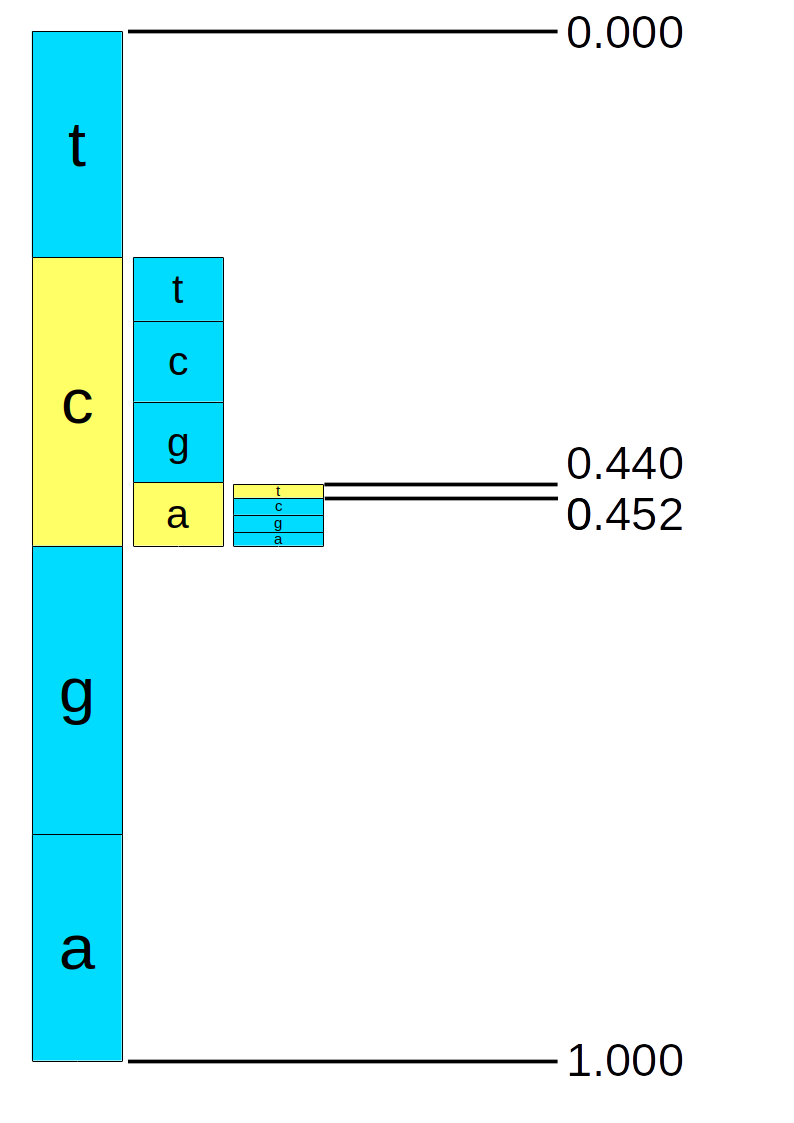
\includegraphics[height=250pt, keepaspectratio=true]{img/range_code.png}

Decoding is simply the reverse of this.  In the above picture we can see that 0.45 would read off `c', `a' and `t' by repeatedly comparing the symbol ranges to the current range and using those to identify the symbol and produce a new range.

\begin{threeparttable}[t]
\begin{tabular}{rrrr}
\hline
\textbf{Range low} & \textbf{Range high} & \textbf{Fraction into range} & \textbf{Symbol}\\
\hline
0.000 & 1.000 & 0.450 & c\\
0.200 & 0.500 & 0.833\tnote{\textbf{a}} & a\\
0.440\tnote{\textbf{b}} & 0.500 & 0.167 & t\\
\hline
\end{tabular}
\begin{tablenotes}
\item{\textbf{a.}} 0.45 into range 0.2 to 0.5: $(0.45-0.2)/(0.5-0.2) = 0.833$.
This falls within the 0.8 to 1.0 symbol range for `a'.
\item{\textbf{b.}} `a' symbol range 0.8 to 1.0 applied to range 0.2 to 0.5:  $0.2+0.8\times(0.5-0.2) = 0.44$ and $0.2+1.0\times(0.5-0.2) = 0.5$.
\end{tablenotes}
\end{threeparttable}

Note: The above example not how the actual implementation works\footnote{This implementation was designed by Eugene Shelwein, based on Michael Schindler's earlier work.}.
For efficiency, we use integer values having a starting range of 0 to $2^{32}-1$.
We write out the top 8-bits of the range when low and high become the same value.
Special care needs to be taken to handle small values are are numerically close but stradding a top byte value, such as 0x37ffba20 to 0x38000034.
The decoder does not need to do anything special here, but the encoder must track the number of 0xff or 0x00 values to emit in order to avoid needing arbitrary precision integers.

Pseudocode for the range codec decoding follows.
This implementation uses code (next few bytes in the current bit-stream) and range instead of low and high, both 32-bit unsigned integers.
This specification focuses on decoding, but given the additional complexity of the precision overflows in encoder we describe this implementation too.

\textsc{RangeDecodeCreate} initialises the range coder, reading the first bytes of the compressed data stream.

\begin{algorithmic}[1]
\Function{RangeDecodeCreate}{}
  \settowidth{\maxwidth}{range\ }
  %\State \algalign{low}{\gets} $0$\Comment{32-bit unsigned}
  \State \algalign{range}{\gets} $2^{32}-1$\Comment{Maximum 32-bit unsigned value}
  \State \algalign{code}{\gets} $0$\Comment{32-bit unsigned}
  \For{$i \gets 0$ to $4$}
    \State $code \gets (code \shiftl 8) + $\Call{ReadUint8}{}
  \EndFor
  \State $code \gets code \bitand 2^{32}-1$
  \State \Return this range coder ($range$, $code$)
\EndFunction
\end{algorithmic}

Decoding each symbol is in two parts; getting the current frequency and updating the range.

\begin{algorithmic}[1]
\Function{RangeGetFreq}{$tot\_freq$}
  \State $range \gets range \bdiv tot\_freq$
  \State \Return $code \bdiv range$
\EndFunction
\end{algorithmic}

\begin{algorithmic}[1]
\Procedure{RangeDecode}{$sym\_low, sym\_freq, tot\_freq$}
  \settowidth{\maxwidth}{range\ }
  \State \algalign{code}{\gets} $code - sym\_low \times range$
  \State \algalign{range}{\gets} $range \times sym\_freq$

  \While{$range < 2^{24}$} \Comment{Renormalise}
    \settowidth{\maxwidth}{range\ }
    \State \algalign{range}{\gets} $range \shiftl 8$
    \State \algalign{code}{\gets} $(code\shiftl8) + $\Call{ReadUint8}{}
  \EndWhile
\EndProcedure
\end{algorithmic}

As mentioned above, the encoder is more complex as it cannot shift out the top byte until it has determined the value.
This can take a considerable while if our current low / high (low + range) are very close but span a byte boundary, such as 0x37ffba20 to 0x38000034, where ultimately we will later emit either 0x37 or 0x38.
To handle this case, when the range gets too small but the top bytes still differ, the encoder caches the top byte of low (0x37) and keeps track of how many 0xff or 0x00 values will need to be written out once we finally observe which value the range has shrunk to.

The \textsc{RangeEncode} function is a straight forward reversal of the \textsc{RangeDecode}, with the exception of the special code for shifting the top byte out of the $low$ variable.

\begin{algorithmic}[1]
\Procedure{RangeEncode}{$sym\_low, sym\_freq, tot\_freq$}
  \settowidth{\maxwidth}{old\_low\ }
  \State \algalign{old\_low}{\gets} $low$
  \State \algalign{range}{\gets} $range \bdiv tot\_freq$
  \State \algalign{low}{\gets} $low + sym\_low \times range$
  \State \algalign{range}{\gets} $range \times sym\_freq$

  \Statex
  \If{low < old\_low}
    \State $carry \gets 1$ \Comment{overflow}
  \EndIf
  \While{$range < 2^{24}$} \Comment{Renormalise}
    \settowidth{\maxwidth}{range\ }
    \State \algalign{range}{\gets} $range \shiftl 8$
    \State \Call{RangeShiftLow}{}
  \EndWhile
\EndProcedure
\end{algorithmic}

\textsc{RangeShiftLow} is the main heart of the encoder renormalisation.
It tracks the total number of extra bytes to emit and $carry$ indicates whether they are a string of 0xFF or 0x00 values.

\begin{algorithmic}[1]
\Procedure{RangeShiftLow}{}
  \If{$low < $ 0xff000000 $\logor carry \ne 0$}
    \If{$carry = 0$}
      \State \Call{WriteByte}{$cache$} \Comment{top byte $cache$ plus FFs}
      \While{$FFnum > 0$}
        \State \Call{WriteByte}{0xff}
        \State $FFnum \gets FFnum - 1$
      \EndWhile
    \Else
      \State \Call{WriteByte}{$cache + 1$} \Comment{top byte $cache+1$ plus 00s}
      \While{$FFnum > 0$}
        \State \Call{WriteByte}{0}
        \State $FFnum \gets FFnum - 1$
      \EndWhile
    \EndIf
    \State $cache \gets low \shiftr 24$ \Comment{Copy of top byte ready for next flush}
    \State $carry \gets 0$
  \Else
    \State $FFnum \gets FFnum + 1$
  \EndIf
  \Statex
  \State $low \gets low \shiftl 8$
\EndProcedure
\end{algorithmic}

For completeness, the Encoder initialisation and finish functions are below.

\begin{algorithmic}[1]
\Procedure{RangeEncodeStart}{}
  \settowidth{\maxwidth}{FFnum\ }
  \State \algalign{low}{\gets} $0$
  \State \algalign{range}{\gets} $2^{32}-1$
  \State \algalign{FFnum}{\gets} $0$
  \State \algalign{carry}{\gets} $0$
  \State \algalign{cache}{\gets} $0$
\EndProcedure
\end{algorithmic}

\begin{algorithmic}[1]
\Procedure{RangeEncodeEnd}{}
  \For{$i \gets 0$ to $4$} \Comment{Flush any residual state in $low$}
    \State \Call{RangeShiftLow}{}
  \EndFor
\EndProcedure
\end{algorithmic}


\subsection{Statistical Modelling}

The probabilities passed to the range coder may be fixed for all scenarios (as we had in the ``cat'' example), or they may be adaptive and context aware.
For example the letter `u' occurs around 3\% of time in English text, but if the previous letter was `q' it is close to 100\% and if the previous letter was `u' it is close to 0\%.
Using the previous letter is known as an Order-1 entropy encoder, but the context can be anything.
We can also adaptively adjust our probabilities as we encode or
decode, learning the likelihoods and thus avoiding needing to store
frequency tables in the data stream covering all possible contexts.

To do this we use a statistical model, containing an array of symbols $S$ and their frequencies $F$.
The sum of these frequences must be less than $2^{16}-32$.
When they get too high, they are renormalised by approximately halving the frequencies (ensuring none drop to zero).

Typically an array of models are used where the array index represents the current context.

To encode any symbol the entropy encoder needs to know the frequency of the symbol to encode, the cumulative frequencies of all symbols prior to this symbol, and the total of all frequencies.
For decoding a cumulative frequency is obtained given the frequency total and the appropriate symbol is found matching this frequency.
Symbol frequencies are updated after each encode or decode call and the symbols are kept in order of most-frequent symbol first in order to  reduce the overhead of scanning through the cumulative frequencies.

\textsc{ModelCreate} initialises a model by setting every symbol to have a frequency of 1.
(At no point do we permit any symbol to have zero frequency.)

\begin{algorithmic}[1]
\Function{ModelCreate}{$num\_sym$}
  \State $total\_freq \gets num\_sym$
  \State $max\_sym \gets num\_sym-1$
  \For{$i \gets 0$ to $max\_sym$}
    \State $S_i \gets i$
    \State $F_i \gets 1$
  \EndFor
  \State \Return this model ($total\_freq$, $max\_sym$, $S$, $F$)
\EndFunction
\end{algorithmic}

\textsc{ModelDecode} is called once for each decoded symbol.
It returns the next symbol and updates the model frequencies automatically.

\begin{algorithmic}[1]
\Function{ModelDecode}{rc}
  \State $freq \gets$ $rc.$\Call{RangeGetFrequency}{$total\_freq$}
  \State $x \gets 0$
  \State $acc \gets 0$
  \While{$acc + F_x \le freq$}
    \State $acc \gets acc + F_x$
    \State $x \gets x+1$
  \EndWhile
  \State $rc.$\Call{RangeDecode}{$acc,\ F_x,\ total\_freq$}
  \State $F_x \gets F_x + 16$ \Comment{Update model frequencies}
  \State $total\_freq \gets total\_freq + 16$
  \If{$total\_freq > 2^{16}-17$}
    \State \Call{ModelRenormalise}{}
  \EndIf
  \State $sym \gets S_x$
  \If{$x > 0 \logand F_x > F_{x-1}$}
    \State \Call{Swap}{$F_x$, $F_{x-1}$}
    \State \Call{Swap}{$S_x$, $S_{x-1}$}
  \EndIf
  \State \Return $sym$
\EndFunction
\end{algorithmic}

\textsc{ModelRenormalise} is called whenever the total frequencies get too high.
The frequencies are halved, taking sure to avoid any zero frequencies being created.

\begin{algorithmic}[1]
\Procedure{ModelRenormalise}{}
  \State $total\_freq \gets 0$
  \For{$i \gets 0$ to $max\_sym$}
    \State $F_i \gets F_i - (F_i \bdiv 2)$
    \State $total\_freq \gets total\_freq + F_i$
  \EndFor
\EndProcedure
\end{algorithmic}

\subsection{Order-0 and Order-1 Encoding}

We can combine the model defined above and the range coder to provide a simple function to perform Order-0 entropy decoder.

\begin{algorithmic}[1]
\Function{DecodeOrder0}{$len$}
  \State $max\_sym \gets $\Call{ReadUint8}{}
  \If{$max\_sym = 0$}
    \State $max\_sym \gets 256$
  \EndIf
  \State $model\_lit \gets $\Call{ModelCreate}{$max\_sym$}
  \Statex
  \State $rc \gets $\Call{RangeDecodeCreate}{}
  \For{$i \gets 0$ to $len-1$}
    \State $out_i \gets model\_lit.$\Call{ModelDecode}{$rc$}
  \EndFor
  \State \Return $out$
\EndFunction
\end{algorithmic}

The Order-1 variant simply uses an array of models and selects the appropriate model based on the previous value encoded or decoded.
This array index is our ``context''.

\begin{algorithmic}[1]
\Function{DecodeOrder1}{$len$}
  \State $max\_sym \gets $\Call{ReadUint8}{}
  \If{$max\_sym = 0$}
    \State $max\_sym \gets 256$
  \EndIf
  \For{$i \gets 0$ to $max\_sym-1$}
    \State $model\_lit_i \gets $\Call{ModelCreate}{$max\_sym$}
  \EndFor
  \Statex
  \State $rc \gets $\Call{RangeDecodeCreate}{}
  \State $last \gets 0$
  \For{$i \gets 0$ to $len-1$}
    \State $out_i \gets model\_lit_{last}.$\Call{ModelDecode}{$rc$}
    \State $last \gets out_i$
  \EndFor
  \State \Return $out$
\EndFunction
\end{algorithmic}

\subsection{RLE with Order-0 and Order-1 Encoding}

The \textsc{DecodeOrder0} and \textsc{DecodeOrder1} codecs can be expanded to include a count of how many runs of each symbol should be decoded.
Both order 0 and order 1 variants are possible.

After the symbol is decoded, the run length must be decoded to
indicate how many \emph{extra} copies of this symbol occur.  Long runs
are broken into a series of lengths of no more than 3.  If length 3
is decoded it indicates we must decode an additional length and add to
the current one.  The context used for the run length model is the
symbol itself for the initial run, 256 for the first continuation run
(if $\ge 4$) and 257 for any further continuation runs.  Thus encoding
10 `A' characters would first store symbol `A' followed by run length
3 (with context `A'), length 3 (context 256), length 3 (context
257), and length 1 (context 258).

For example, if we have the string ``RRRRUNN'' we will decode
symbol `R' run 3, symbol `U' run 0, symbol `N' run 1.

\begin{algorithmic}[1]
\Function{DecodeRLE0}{$len$}
  \State $max\_sym \gets $\Call{ReadUint8}{}
  \If{$max\_sym = 0$}
    \State $max\_sym \gets 256$
  \EndIf
  \State $model\_lit \gets $\Call{ModelCreate}{$max\_sym$}

  \For{$i \gets 0$ to $257$}
    \State $model\_run_i \gets $\Call{ModelCreate}{$4$}
  \EndFor
  \Statex
  \State $rc \gets $\Call{RangeDecodeCreate}{}
  \State $i \gets 0$
  \While{$i < len$}
    \State $out_i \gets model\_lit.$\Call{ModelDecode}{$rc$}
    \State $part \gets model\_run_{out_i}.$\Call{ModelDecode}{$rc$}
    \State $run \gets part$
    \State $rctx \gets 256$
    \While{$part = 3$}
      \State $part \gets model\_run_{rctx}.$\Call{ModelDecode}{$rc$}
      \State $rctx \gets 257$
      \State $run \gets run + part$
    \EndWhile
    \For{$j \gets 1$ to $run$}
      \State $out_{i+j} \gets out_i$
    \EndFor
    \State $i \gets run+1$
  \EndWhile
  \State \Return $out$
\EndFunction
\end{algorithmic}

The order-1 run length variant is identical to order-0 except the
previous symbol is used as the context for the next literal.  The
context for the run length does not change.

\begin{algorithmic}[1]
\Function{DecodeRLE1}{$len$}
  \State $max\_sym \gets $\Call{ReadUint8}{}
  \If{$max\_sym = 0$}
    \State $max\_sym \gets 256$
  \EndIf
  \For{$i \gets 0$ to $max\_sym-1$}
    \State $model\_lit_i \gets $\Call{ModelCreate}{$max\_sym$}
  \EndFor
  \For{$i \gets 0$ to $257$}
    \State $model\_run_i \gets $\Call{ModelCreate}{$4$}
  \EndFor
  \Statex
  \State $rc \gets $\Call{RangeDecodeCreate}{}
  \State $last \gets 0$
  \State $i \gets 0$
  \While{$i < len$}
    \State $out_i \gets model\_lit_{last}.$\Call{ModelDecode}{$rc$}
    \State $last \gets out_i$
    \State $part \gets model\_run_{last}.$\Call{ModelDecode}{$rc$}
    \State $run \gets part$
    \State $rctx \gets 256$
    \While{$part = 3$}
      \State $part \gets model\_run_{rctx}.$\Call{ModelDecode}{$rc$}
      \State $rctx \gets 257$
      \State $run \gets run + part$
    \EndWhile
    \For{$j \gets 1$ to $run$}
      \State $out_{i+j} \gets last$
    \EndFor
    \State $i \gets run+1$
  \EndWhile
  \State \Return $out$
\EndFunction
\end{algorithmic}

%\subsection{General Purpose Entropy Encoder}

We wrap up the Order-0 and 1 entropy encoder, both with and without run length encoding, into a data stream that specifies the type of encoded data and also permits a number of additional transformations to be applied.
These transformations support bit packing (for example a data block with only 4 distinct values can be packed with 4 values per byte), no-op for tiny data blocks where entropy encoding would grow the data and N-way interleaving of the 8-bit components of a 32-bit value.

\begin{table}[h]
\centering
\begin{tabular}{|r|r|r|r|p{9cm}|l|}
\hline
\multicolumn{2}{|r|}{\textbf{Bits} } & \textbf{Type}  & \textbf{Name} & \multicolumn{2}{p{9cm}|}{\textbf{Description}} \\
\hline
\multicolumn{2}{|r|}{8} & uint8 & $flag$ & \multicolumn{2}{p{9cm}|}{Data format bit field}\\
\cline{1-6}

\multicolumn{6}{|l|}{}\\[-0.3em]
\multicolumn{6}{|l|}{\textit{Unless \textsc{NoSize} flag is set:} } \\
\cline{2-5}
& ? & uint7 & ulen & Uncompressed length & \\
\cline{2-5}

\multicolumn{6}{|l|}{}\\[-0.3em]
\multicolumn{6}{|l|}{\textit{If \textsc{Stripe} flag is set:} } \\
\cline{2-5}
& ? & uint8 & N & Number of sub-streams & \\
& ? & uint7[] & clen[] & N copies of compressed sub-block length & \\
& ? & uint8[] & cdata[] & N copies of Compressed data sub-block (recurse) & \\
\cline{2-5}

\multicolumn{6}{|l|}{}\\[-0.7em]
\multicolumn{6}{|l|}{\textit{If \textsc{Cat} flag is set (and \textsc{Stripe} flag is unset):} } \\
\cline{2-5}
& ? & uint8[] & udata & Uncompressed data stream & \\
\cline{2-5}

\multicolumn{6}{|l|}{}\\[-0.7em]
\multicolumn{6}{|l|}{\textit{If \textsc{Pack} flag is set (and neither \textsc{Stripe} or \textsc{Cat} flags are set):} } \\
\cline{2-5}
& ? & uint8[] & pack\_meta & Pack lookup table & \\
\cline{2-5}

\multicolumn{6}{|l|}{}\\[-0.7em]
\multicolumn{6}{|l|}{\textit{If neither \textsc{Stripe} or \textsc{Cat} flags are set:} } \\
\cline{2-5}
& ? & uint8[] & cdata & Entropy encoded data stream (see \textsc{Order} / \textsc{RLE} / \textsc{Ext} flags) & \\
\cline{2-5}
\multicolumn{6}{|l|}{}\\
\hline
\end{tabular}
\end{table}

The first byte of our generalised data stream is a bit-flag detailing the type of transformations and entropy encoders to be combined, followed by optional meta-data, followed by the actual compressed data stream.
The bit-flags are defined below, but note not all combinations are permitted.

\begin{threeparttable}[t]
\begin{tabular}{llll}
\hline
\textbf{Bit AND value} & \textbf{Code} & \textbf{Description} \\
\hline
1 & \textsc{Order}\tnote{\textbf{a}} & Order-0 or Order-1 entropy coding. \\
2 & reserved & Reserved (for possible order-2/3)\\
4 & \textsc{Ext} & ``External'' compression via bzip2\\
8 & \textsc{Stripe}\tnote{\textbf{b}} & N-way interleaving of byte streams.\\
16 & \textsc{NoSize} & original size is not recorded (used by \textsc{Stripe})\\
32 & \textsc{Cat}\tnote{\textbf{b}} & Data is uncompressed\\
64 & \textsc{RLE}\tnote{\textbf{a}} & Run length encoding, with runs and literals encoded separately\\
128 & \textsc{Pack} & Pack 2, 4, 8 or infinite symbols per byte.\\
\hline
\end{tabular}
\begin{tablenotes}
\item{\textbf{a.}} Has no effect when \textsc{Ext} flag is set.
\item{\textbf{b.}} Not to be used in conjunction with other flags
  except \textsc{Pack} and \textsc{NoSize}.
\end{tablenotes}
\end{threeparttable}

Of these \textsc{Stripe} is the most complex.
As with the rANS4x16 encoder, the data is rearranged such that every
$N^{th}$ byte is adjacent in a single block producing N distinct sub-blocks.
Each of the N streams is then itself compressed using this compression format.

For example an input block of small unsigned 32-bit little-endian numbers may use RLE for the first three streams as they are mostly zero, and a non-RLE Order-0 entropy encoder of the last stream.
Normally our data format will include the decoded size, but with \textsc{Stripe} we can omit this from the internal compressed streams as we know their size will be a computable fraction of the combined data.

The data layout differs for each of these bit types, as described below in the \textsc{ArithDecode} function.
Some of these can be used in combination, so the order needs to be observed.
The Pack format has additional meta data.
This is decoded first, before entropy decoding and finally expanding thespecified pack transformation after decompression.
For example value 193 is indicates a byte stream should be decoded with an RLE aware order-1 entropy encoder and then unpacked.

\begin{algorithmic}[1]
\Function{ArithDecode}{$len$}
  \State $flags \gets $\Call{ReadUint8}{}
  \If{$flags \bitand$ \textsc{NoSize} $\ne 0$}
    \State $len \gets$\Call{ReadUint7}{}
  \EndIf
  \If{$flags \bitand$ \textsc{Stripe}}
    \State $data \gets $\Call{DecodeSTRIPE}{$len$}
    \State \Return $data$
  \EndIf{}
  \If{$flags \bitand$ \textsc{Pack}}
    \State $pack\_len \gets len$
    \State $(P,\ nsym,\ len) \gets $\Call{DecodePackMeta}{}
  \EndIf
  \Statex \Comment{Entropy Decoding}
  \If{$flags \bitand$ \textsc{Cat}}
    \State $data \gets $\Call{ReadData}{$len$}
  \ElsIf{$flags \bitand$ \textsc{Ext}}
    \State $data \gets $\Call{DecodeEXT}{$len$}
  \ElsIf{$flags \bitand$ \textsc{RLE}}
    \If{$flags \bitand$ \textsc{Order}}
      \State $data \gets $\Call{DecodeRLE1}{$len$}
    \Else
      \State $data \gets $\Call{DecodeRLE0}{$len$}
    \EndIf
  \Else
    \If{$flags \bitand$ \textsc{Order}}
      \State $data \gets $\Call{DecodeOrder1}{$len$}
    \Else
      \State $data \gets $\Call{DecodeOrder0}{$len$}
    \EndIf
  \EndIf
  \Statex \Comment{Apply data transformations}
  \If{$flags \bitand$ \textsc{Pack}}
    \State $data \gets $\Call{DecodePack}{$data$, $P$, $nsym$, $pack\_len$}
  \EndIf
  \State \Return $data$
  \EndFunction
\end{algorithmic}

The specifics of each sub-format are described below, in the order (minus meta-data specific shuffling) they are applied.

\begin{itemize}
\item{\textbf{\textsc{Stripe}}:}
The byte stream consists of a 7-bit encoded uncompressed length and a
byte holding the number of substreams $N$, and their 7-bit encoded
compressed data streams lengths.  This is then followed by the
substreams themselves, each of which is a valid $cdata$ stream as
defined above, hence this offers a recursive mechanism as each
substream has its own format byte.

The total uncompressed byte stream is then an interleaving of one byte
in turn from each of the N substreams (in order of 1st to Nth).  Thus
an array of 32-bit unsigned integers could be unpacked using
\textsc{Stripe} to compress each of the 4 8-bit components together with
their own algorithm.

\begin{algorithmic}[1]
\Function{RansDecodeStripe}{$len$}
  \State $N \gets $\Call{ReadUint8}{}
  \For{$j \gets 0$ to $N$} \Comment{Fetch N compressed lengths}
    \State $clen_j \gets $\Call{ReadUint7}{}
  \EndFor
  \Statex
  \For{$j \gets 0$ to $N$} \Comment{Decode N streams}
    \State $ulen_j \gets (len \bdiv N) + ((len \bmod N) > j)$
\Comment{$(x > y)$ expression being 1 if true, 0 if false}
    \State $T_j \gets $\Call{ArithDecode}{$ulen_j$}
  \EndFor
  \Statex
%  \For{$i \gets 0$ to $len - 1$} \Comment{Interleave}
%    \State $out_i \gets T_{(i \bmod N),\ (i \bdiv N)}$
%  \EndFor
  \For{$j \gets 0$ to $N - 1$} \Comment{Interleave}
    \For{$i \gets 0$ to $ulen_j - 1$}
      \State $out_{i \times N + j} \gets T_{j,i}$
    \EndFor
  \EndFor
  \State \Return $out$
\EndFunction
\end{algorithmic}

\item{\textbf{\textsc{NoSize}}:}
Do not store the size of the uncompressed data stream.
This information is not required when the data stream is one of the four sub-streams in the \textsc{Stripe} format.

\item{\textbf{\textsc{Cat}}:}
If present, all other bit flags should be nul, with the possible
exception of \textsc{NoSize} or \textsc{Pack}.

The uncompressed data stream is the same as the compressed stream.
This is useful for very short data where the overheads of compressing are too high.

\item{\textbf{\textsc{Order}}:}
Bit field defining order-0 (unset) or order-1 (set) entropy encoding, as described above by the \textsc{DecodeOrder0} and \textsc{DecodeOrder1} functions.

\item{\textbf{\textsc{RLE}}:}
Bit field defining whether the Order-0 and Order-1 encoding should also use a run-length.
When set, the \textsc{DecodeRLE0} and \textsc{DecodeRLE1} functions will be used instead of \textsc{DecodeOrder0} and \textsc{DecodeOrder1}.

\item{\textbf{\textsc{Ext}}:}
Instead of using the adaptive arithmetic coder for decompression (with or without RLE), this uses an compression codec defined in an ``external'' library.
Currently the only supported such codec is Bzip2.
In future more may be added, so the magic number \emph{must} be validated to check the codec being used.

Given bzip2 is already supported elsewhere in CRAM, the purpose of adding it here is to permit bzip2 compression after \textsc{Pack} and \textsc{Stripe} transformations.
This may be tidied up in later CRAM releases to clarify the separation between compression codecs and data transforms, but that requires more major restructuring so for compatibility with v3.0 these have been placed into this single codec.

\begin{algorithmic}[1]
\Function{DecodeExt}{$len$}
  \If{Bzip2 magic number is present}
    \State \Return \Call{DecodeBzip2}{$len$}
  \Else
    \State Error
  \EndIf
\EndFunction
\end{algorithmic}

\item{\textbf{\textsc{Pack}}:}
Data containing only 1, 2, 4 or 16 distinct values can have multiple
values packed into a single byte (infinite, 8, 4 or 2).  The distinct
symbol values do not need to be adjacent as a mapping table $P$
converts mapped value $x$ to original symbol $P_x$.

The packed format is split into uncompressed meta-data (below) and the
compressed packed data as described in the rANS 4x16 bit-packing section.
The same \textsc{DecodePackMeta} and \textsc{DecodePack} functions are used.

\end{itemize}

\section{Name tokenisation codec}

Sequence names (identifiers) typically follow a structured pattern and compression based on columns within those structures usually leads to smaller sizes.
The sequence name (identifier) tokenisation relies heavily on the General Purpose Entropy Encoder described above.

As an example, take a series of names:

\begin{verbatim}
I17_08765:2:123:61541:01763#9
I17_08765:2:123:1636:08611#9
I17_08765:2:124:45613:16161#9
\end{verbatim}

We may wish to tokenise each of these into 7 tokens, e.g.
``I17\_08765:2:'', ``123'', ``:'', ``61541'', ``:'', ``01763''and
``\#9''. Some of these are multi-byte strings, some single characters,
and some numeric, possibily with a leading zero.  We also observe some
regularly have values that match the previous line (the initial prefix
string, colons, ``\#9'') while others are numerically very close to the
value in the previous line (124 vs 123).

The name tokeniser compares each name against a previous name (which
is not necessarily the one immediately prior) and encodes this name
either as a series of differences to the previous name or marking it
as an exact duplicate.  A maximum of 128 tokens are permitted within
any single read name.

Token IDs (types) are listed below.

\begin{tabular}{lllp{10cm}}
\hline
\textbf{ID} & \textbf{Type} & \textbf{Value} & \textbf{Description}\\
\hline
 0 & TYPE    & Type    & Used to determine the type of token at a given position. \\
\hline
 5 & DUP     & Integer (distance) & The entire name is a duplicate of an earlier one.  Used in position 0 only.\\
 6 & DIFF    & Integer (distance) & The entire name is differs to earlier ones.  Used in position 0 only.\\
\hline
 1 & STRING  & String  & A nul-terminated string of characters \\
 2 & CHAR    & Byte    & A single character \\
 7 & DIGITS  & $0 \le$ Int $< 2^{32}$ & A numerical value, not containing a leadng zero \\
 3 & DIGITS0 & $0 \le$ Int $< 2^{32}$ & A numerical value possibly starting in leading zeros \\
 4 & DZLEN   & Int length & Length of associated DIGITS0 token.\\
 8 & DELTA  & $0 \le$ Int $< 256$   & A numeric value being stored as the difference to the numeric value of this token on the previous name. \\
 9 & DELTA0 & $0 \le$ Int $< 256$ & As DELTA, but for numeric values starting with leading zeros \\
10 & MATCH   & (none) & This token is identical type and value to the same position in the previous name (NB: not permitted for DELTA/DELTA0)\\
11 & NOP & (none) & Does nothing\\
12 & END     & (none) & Marks end of name\\
\hline
\end{tabular}

The tokens and values are stored in a 2D array of byte streams,
$B_{pos,type}$, where pos 0 is reserved for name meta-data (whether it
is a duplicate name) and pos 1 onwards is for the first, second and
later tokens.  $Type$ is one of the token types listed above,
corresponding to the type of data being stored.  Some token types may
also have associated values.  $B_{pos,\texttt{TYPE}}$ ($type$) holds the token
type itself and that is then used to retrieve any associated
value(s) if appropriate from $B_{pos,type}$.  Thus multiple types at the same token
position will have their values encoded in distinct data streams,
e.g. if position 5 is of type either DIGITS or DELTA then data streams
will exist for $B_{5,\texttt{TYPE}}$, $B_{5,\texttt{DIGITS}}$ and $B_{5, \texttt{DELTA}}$.
Decoding per name continues until a token of type END is observed.

More detail on the token types is given below.

\begin{itemize}
\item{\textbf{TYPE}:}
This is the first token fetched at each token position.  It holds the
type of the token at this position, which in turn may then require
retrieval from type-specific data streams at this position.

For position 0, the TYPE field indicates whether this record is an
exact duplicate of a prior read name or has been encoded as a delta to
an earlier one.

\item{\textbf{DUP}, \textbf{DIFF}:}
These types are fetched for position 0, at the start of each new
identifier.  The value is an integer value describing how many reads
before this (with 1 being the immediately previous name) we are
comparing against.  When we refer to ``previous name'' below, we
always mean the one indicated by the DIFF field and not the one
immediately prior to the current name.

The first record will have a DIFF of zero and no delta or match
operations are permitted.

\item{\textbf{STRING}:}
We fetch one byte at a time from the value byte stream, appending to the
name buffer until the byte retrieved is zero.  The zero byte is not
stored in the name buffer.
For purposes of token type MATCH, a match is defined as entirely
matching the string including its length.

\item{\textbf{CHAR}:}
Fetch one single byte from the value byte stream and append to the name buffer.

\item{\textbf{DIGITS}:}
Fetch 4 bytes from the value byte stream and intrepret these as a little
endian unsigned integer.  This is appended to the name buffer as
string of base-10 digits, most significant digit first.  Larger
values may be represented, but will require multiple DIGITS tokens.
Negative values may be encoded by treating the minus sign as a CHAR or
STRING and storing the absolute value.

\item{\textbf{DIGITS0}, \textbf{DZLEN}:}
This fetches the 4 byte value from $B_{pos,DIGITS0}$ and a 1 byte
length from $B_{pos,DZLEN}$.  As per DIGITS, the value is intrepreted as a
little endian unsigned integer.  The length indicates the total
size of the numeric value when displayed in base 10 which must be
greater than $\log_{10}(value)$ with any remaining length indicating
the number of leading zeros.  For example if DIGITS0 value is 123 and
DZLEN length is 5 the string ``00123'' must be appended to the name.

For purposes of the MATCH type, both value and length must match.

\item{\textbf{DELTA}:}
Fetch a 1 byte value and add this to the DIGITS value from the
previous name.
The token in the prior name must be of type DIGITS or DELTA.

MATCH is not supported for this type.

\item{\textbf{DELTA0}:}
As per DELTA, but the 1 byte value retrieved is added to the DIGITS0
value in the previous name.  No DZLEN value is retrieved, with the
length from the previous name being used instead.
The token in the prior name must be of type DIGITS0 or DELTA0.

MATCH is not supported for this type.

\item{\textbf{MATCH}:}
This token matches the token at the same position in the previous
name.  (The previous name is permitted to also have a MATCH token at
this position, in which case it recurses to its previous name.)

MATCH is only valid when the token being matched against is CHAR,
STRING, DIGITS, DIGITS0 or MATCH.  (I.e. matching a numeric delta will not
repeat the delta increment.)

No value is needed for MATCH tokens.

\item{\textbf{NOP}:}
This token type does nothing.
The purpose of this is simply to permit skipping tokens in order to
keep token numbers in sync, such as when processing ``10'' vs ``-10''
with the latter needing an additional ``-'' token.

\item{\textbf{END}:}
Marks the end of the name.  A nul byte is added to the name output
buffer.  No value is needed for END tokens.
\end{itemize}

Decoding needs some simple functions to read successive bytes from our token byte streams, as 8-bit characters or unsigned integers, as 32-bit unsigned integers and nul-terminated strings.  We reuse the \textsc{ReadUint32} and related functions with the byte array specified as input.

\begin{algorithmic}[1]
\Statex
\Statex \textit{(Convert an integer to a string form in base-10 digits, at least $len$ bytes long with leading zeros)}
\Function{LeftPadNumber}{$val,\ len$}
  \State $str \gets val$ \Comment{Implicit language-specific Integer to String conversion}
  \While{\Call{Length}{$str$} < $len$}
    \State $str \gets$ `$0$' $ \concat str$
  \EndWhile
  \State \Return $str$
\EndFunction
\end{algorithmic}

For the main name decoding loop, we use a single dimensional array of
names decoded so far, $N$, and a two dimensional array of their tokens
$T$ (indexed by name number $n$ and token position $t$ within that
name).  We define a function to decode the $n^{th}$ name ($N_n$) using
a previous $m^{th}$ name ($N_m$).  The tokens $T$ are used in
\texttt{MATCH} and \texttt{DELTA} token types to copy data from when
constructing the name.

Now we have the basic primitives for pulling from the $B$ byte
streams, decoding the $n^{th}$ individual name is as
follows\footnote{For simplicity of algorithm description, we take a
  flexible approach as to whether we read/write $T$ in numeric or
  string form.  For example a \texttt{DELTA} token will fetch the
  previous token as a string, interpret it as a numeric value, add to
  it, and then write it back as a string.  Practical implementations
  may wish to separate out T into distinct integer and string
  arrays.}:


\begin{algorithmic}[1]
\Statex
\Statex \textit{(Decodes the $n^{th}$ name, returning $N_n$ and updating globals $N_n$ and $T_n$)}
\Function{DecodeSingleName}{$n$}
  \State $type \gets$ \Call{ReadUint8}{$B_{0,\textit{TYPE}}$}
  \State $dist \gets$ \Call{ReadUint32}{$B_{0,type}$}
  \State $m \gets n-dist$
  \If{$type = $ \texttt{DUP}}
    \State $N_n \gets N_m$
    \State $T_n \gets T_m$ \Comment{Copy for all $T_{n,*}$}
    \State \Return $N_n$
  \EndIf
  \Statex
  \State $t \gets 1$ \Comment{Token number $t$}
  \Repeat
    \State $type \gets$ \Call{ReadUint8}{$B_{t,\texttt{TYPE}}$}
    \If{$type = $ \texttt{CHAR}}
      \State $T_{n,t} \gets$ \Call{ReadChar}{$B_{t,\texttt{CHAR}}$}
    \ElsIf{$type = $ \texttt{STRING}}
      \State $T_{n,t} \gets$ \Call{ReadString}{$B_{t,\texttt{STRING}}$}
    \ElsIf{$type = $ \texttt{DIGITS}}
      \State $T_{n,t} \gets$ \Call{ReadUint32}{$B_{t,\texttt{DIGITS}}$}
    \ElsIf{$type = $ \texttt{DIGITS0}}
      \State $d \gets$ \Call{ReadUnt32}{$B_{t,\texttt{DIGITS0}}$}
      \State $l \gets$ \Call{ReadUint8}{$B_{t,\texttt{DZLEN}}$}
      \State $T_{n,t} \gets$ \Call{LeftPadNumber}{$d,\ l$}
    \ElsIf{$type = $ \texttt{DELTA}}
      \State $T_{n,t} \gets T_{m,t} + $ \Call{ReadUint8}{$B_{t,\texttt{DELTA}}$}
    \ElsIf{$type = $ \texttt{DELTA0}}
      \State $d \gets T_{m,t} + $ \Call{ReadUint8}{$B_{t,\texttt{DELTA0}}$}
      \State $l \gets$ \Call{Length}{$T_{m,t}$} \Comment{String length including leading zeros}
      \State $T_{n,t} \gets$ \Call{LeftPadNumber}{$d,\ l$}
    \ElsIf{$type = $ \texttt{MATCH}}
      \State $T_{n,t} \gets T_{m,t}$
    \Else
      \State $T_{n,t} \gets$\ `'
    \EndIf
    \State $N_n \gets N_n \concat T_{n,t}$
    \State $t \gets t+1$
  \Until{$type = $ \texttt{END}}
  \State \Return $N_n$
\EndFunction
\end{algorithmic}

Given a complex name with both position and type specific values, this
can lead to many separate data streams.  The name tokeniser codec is
a format within a format, as the multiple byte streams $B_{pos,type}$
are serialised into a single byte stream.

The serialised data stream starts with two unsigned little endiand 32-bit
integers holding the total size of uncompressed name buffer and the
number of read names.  This is followed the array elements
themselves.

Token types, $ttype$ holds one of the token ID values listed above
in the list above, plus special values to indicate certain additional
flags.  Bit 6 (64) set indicates that this entire token data stream is a
duplicate of one earlier.  Bit 7 (128) set indicates the token
is the first token at a new position.  This way we only need to store
token types and not token positions.

The total size of the serialised stream needs to be already known, in
order to determine when the token types finish.

\begin{tabular}{|r|r|r|l|l|p{10cm}|}
\hline
\multicolumn{3}{|r|}{\textbf{Bytes}} & \textbf{Type} & \textbf{Name} & \textbf{Description}\\
\hline
\multicolumn{3}{|r|}{4} & uint32 & $uncomp\_length$ & Length of uncompressed name buffer\\
\multicolumn{3}{|r|}{4} & uint32 & $num\_reads$ & Number of read names\\
\multicolumn{3}{|r|}{1} & uint8  & $use\_arith$ & Whether compression is arithmetic (1) or rANS4x16 (0)\\
\hline
\multicolumn{6}{|l|}{\quad\textit{For each token data stream}}\\
\cline{2-6}
& \multicolumn{2}{r|}{1} & uint8 & $ttype$ & Token type code plus flags (64=duplicate, 128=next token position).\\
\cline{2-6}
& \multicolumn{5}{l|}{\textit{If ttype AND 64 (duplicate)}}\\
\cline{3-6}
& & 1 & uint8 & $dup\_pos$  & Duplicate from this token position\\
& & 1 & uint8 & $dup\_type$ & Duplicate from this token type ID\\
\cline{3-6}
& \multicolumn{5}{l|}{\textit{else if not duplicate}}\\
\cline{3-6}
& & ? & i7 & $clen$ & compressed length (7-bit encoding)\\
& & $clen$ & $cdata$ & stream & compressed data stream\\
\hline
\end{tabular}

A few tricks are used to remove some byte streams.  In addition to the explicit marking of duplicate bytes streams, if a byte stream of token types is entirely MATCH apart from the very first value it is discarded.  It is possible to regenerate this during decode by observing the other byte streams.  For example if we have a byte stream $B_{5,DIGITS}$ but no $B_{5,TYPE}$ then we assume the contents of $B_{5,TYPE}$ consist of one DIGITS type followed by as many MATCH types as are needed.

The $cdata$ stream itself is as described in the General Purpose Entropy Encoder section above, with the \textsc{ArithDecode} function.

\begin{algorithmic}[1]
\Statex
\Statex \textit{(Decodes and uncompressed the serialised token byte streams)}
\Function{DecodeTokenByteStreams}{$use\_arith$}
  \State $sz \gets 0$
  \State $t \gets -1$
  \Repeat
    \State $ttype \gets$ \Call{ReadUint8}{}
    \State $tok\_new \gets ttype \bitand 128$
    \State $tok\_dup \gets ttype \bitand 64$
    \State $type \gets ttype \bitand 63$
    \If{$tok\_new \ne 0$}
      \State $t \gets t+1$
      \If{$type \ne \texttt{TYPE}$}
        \State $B_{t,\texttt{TYPE}} \gets (type, \texttt{TOK\_MATCH}, \texttt{TOK\_MATCH}, ...)$\Comment{for $nnames-1$ times}
      \EndIf
    \EndIf
    \Statex
    \If{$tok\_dup \ne 0$}
       \State $dup\_pos \gets$ \Call{ReadUint8}{}
       \State $dup\_type \gets$ \Call{ReadUint8}{}
       \State $B_{t,type} \gets B_{dup\_pos,dup\_type}$
    \Else
      \State $clen \gets$ \Call{ReadUint7}{}
      \State $data \gets$ \Call{ReadData}{$clen$}
      \If{$use\_arith$}
        \State $B_{t,type} \gets$ \Call{ArithDecode}{}
      \Else
        \State $B_{t,type} \gets$ \Call{RansDecode4x16}{}
      \EndIf
    \EndIf
  \Until{\Call{EOF}{}}
  \State \Return $B$
\EndFunction
\end{algorithmic}

\begin{algorithmic}[1]
\Statex
\Statex \textit{(Decodes the $n^{th}$ name, returning $N_n$ and updating $N_n$ and $T_n$)}
\Function{DecodeNames}{}
  \State $ulen \gets$ \Call{ReadUint32}{}
  \State $nnames \gets$ \Call{ReadUint32}{}
  \State $use\_arith \gets$ \Call{ReadUint8}{}
  \State $B \gets$ \Call{DecodeTokenByteStreams}{$use\_arith$}

  \For{$n \gets 0$ to $nnames-1$}
    \State $N_n \gets$ \Call{DecodeSingleName}{$n$}
  \EndFor
  \State \Return $N$
\EndFunction
\end{algorithmic}


\section{FQZComp quality codec}

% Ideas to explore and TODO list:
%
% 1. Move param do_rev to global part.  It's all or nothing
%
% 2. Delta updates immediately on base 0 to base 1.  Maybe delay
%    initialisation so prevq is 1st base qual.
%
% 3. ReadArray pseudocode needs fixing.
%
% 4. Add param sel_offset to subtract from decoded sel.
%    Eg if we have 2 params and max_sel 3 (0..3) then we may want
%    sel 0/1 for 1st param and sel 0/1 (sel_offset 2) for 2nd?
%
% 5. Add len_bytes to param so we don't need Model_len[4] always.
%
% 6. Permit do_term and term_sym to put in newlines (or whatever)
%    after each record. (See 7 below for example)
%
% 7. Add dmap to apply to quals before doing the prevq != q check.
%    Reason is maybe we're not compressing qualities!  Eg SA:Z: tag
%    may be best using dmap , = 1 and everything else = 0.  Then
%    ``chr4,100,5,blah''; becomes delta 000012223456666.  dtab to
%    divide by 2 then allows it to track token number.
%    Each semi-colon separated text is a new record (qlen) and they're
%    joined together with term_sym (6. above).
%
% 8. Consider adding selector as context for model len, rev and dup.
%    This is important on mixed data sets.  Do we want full sel, or
%    quantised stab[sel]?

The FQZComp quality codec uses an adaptive statistical model to
predict the next quality value in a given context (comprised of
previous quality values, position along this sequence, whether the
sequence is the second in a pair, and a running total of number of
times the quality has changed in this sequence).

For each quality value, the models produce probabilities for all
possible next quality values, which are passed into an arithmetic
entropy encoder to encode or decode the actual next quality value.
The models are then updated based on the actual next quality in order
to learn the statistical properties of the quality data stream.  This
step wise update process is identical for both encoding and decoding.

The algorithm is a generalisation on the original fqzcomp program,
described in \textit{Compression of FASTQ and SAM Format Sequencing
  Data} by Bonfield JK, Mahoney MV (2013). PLoS ONE 8(3):
e59190. \url{https://doi.org/10.1371/journal.pone.0059190}

\subsection{FQZComp Models}

The FQZComp process utilises knowledge of the read lengths, complement
(qualities reversed) status, and a generic parameter selector, but in
order to maintain a strict separation between CRAM data series this
knowledge is stored (duplicated) within the quality data stream
itself.  Note the complement model is only needed in CRAM 3.1 as CRAM
4 natively stores the quality in the original orientation already.
Both reversed and duplication models have no context and are boolean
values.

The parameter selector model also has no context associated with it
and encodes $max\_sel$ distrinct values.  The selector value may be
quantised further using $stab$ to reduce the selector to fewer
sets of parameters.  This is useful if we wish to use the selector
bits directly in the context using the same parameters.  The selector
is arbitrary and may be used for distinguishing READ1 from READ2, as
a precalculated ``delta'' instead of the running total, distinguishing
perfect alignments from imperfect ones, or any other factor that is
shown to improve quality predictability and increase compression
ratio (average quality, number of mismatches, tile, swathe, proximity
to tile edge, etc).

The quality model has a 16-bit context used to address an array of
$2^{16}$ models, each model permitting $max\_sym$ distinct quality
values.  The context used is defined by the FQZcomp parameters, of
which there may be multiple sets, selected using the selector model.
There are 4 read length models each having $max\_sym$ of 256.  Each
model is used for the 4 successive bytes in a 32-bit length value.

\begin{center}
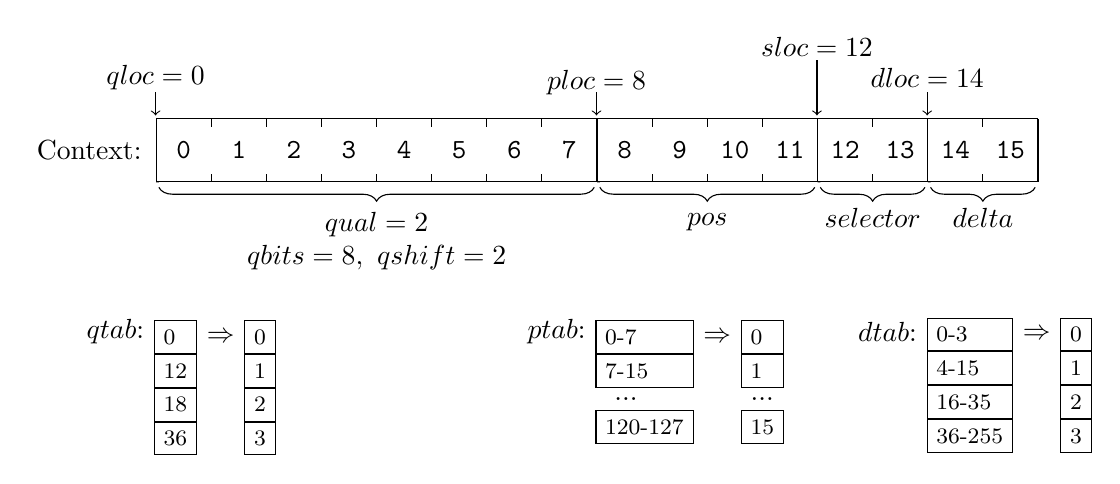
\begin{tikzpicture}[
  boxed/.style={rectangle, draw=black, text width=1cm},
  boxed1/.style={rectangle, draw=black},
  boxed2/.style={rectangle, draw=black, text width=.3cm},
  boxed3/.style={rectangle, draw=black, text width=0.85cm},
]
\newcommand{\x}{0.7cm}
\node at (-0.5, 0) {Context:};
\draw[-] (0*\x+.5*\x,-0.4) -- (0*\x+.5*\x,+0.4);
\foreach \w/\i [count=\n] in {
  3/0, 3/1, 3/2, 3/3, 3/4, 3/5, 3/6, 0/7,   % qual
  3/8, 3/9, 3/10, 0/11,                     % pos
  3/12, 0/13,                               % selector
  3/14, 0/15} {                             % delta
    \draw[-] (\n*\x+.5*\x,-0.4)  -- (\n*\x+.5*\x,-\w/10);
    \draw[-] (\n*\x+.5*\x,\w/10) -- (\n*\x+.5*\x, 0.4);
    \draw[-] (\n*\x-.5*\x,-0.4)  -- (\n*\x+.5*\x,-0.4);
    \draw[-] (\n*\x-.5*\x, 0.4)  -- (\n*\x+.5*\x, 0.4);
    \node(N\n)[minimum height=1cm,minimum width=\x,xshift=\n*\x,font=\ttfamily](N\n){\i};
}
\draw[<-] ([yshift=1pt]N1.north west)+(0,-0.1cm) -- +(0,0.2cm)
    node[yshift=5pt]{$qloc=0$};
\draw[<-] ([yshift=1pt]N9.north west)+(0,-0.1cm) -- +(0,0.2cm)
    node[yshift=3.5pt]{$ploc=8$};
\draw[<-] ([yshift=1pt]N13.north west)+(0,-0.1cm) -- +(0,0.6cm)
    node[yshift=5pt]{$sloc=12$};
\draw[<-] ([yshift=1pt]N15.north west)+(0,-0.1cm) -- +(0,0.2cm)
    node[yshift=5pt]{$dloc=14$};
\draw[decoration={brace,mirror,amplitude=5pt,raise=2pt, post=moveto, pre length=1pt, post length=1pt},decorate]
  (0.5*\x,-0.4) -- node[below=6pt] {\begin{tabular}{c}$qual \shiftl= 2$\\$qbits=8,\ qshift=2$\end{tabular}} +(8*\x,0);
\draw[decoration={brace,mirror,amplitude=5pt,raise=2pt, post=moveto, pre length=1pt, post length=1pt},decorate]
  (8.5*\x,-0.4) -- node[below=8pt] {$pos$} +(4*\x,0);
\draw[decoration={brace,mirror,amplitude=5pt,raise=2pt, post=moveto, pre length=1pt, post length=1pt},decorate]
  (12.5*\x,-0.4) -- node[below=6pt] {$selector$} +(2*\x,0);
\draw[decoration={brace,mirror,amplitude=5pt,raise=2pt, post=moveto, pre length=1pt, post length=1pt},decorate]
  (14.5*\x,-0.4) -- node[below=6pt] {$delta$} +(2*\x,0);

\node[right] (Q) at ([yshift=-1.8cm,xshift=-1cm]N1.south west) {$qtab$:};
\node[above right,boxed2] (Q0) at (Q.south east)  {\footnotesize{0}};
\node[below right,boxed2] (Q1) at (Q0.south west) {\footnotesize{12}};
\node[below right,boxed2] (Q2) at (Q1.south west) {\footnotesize{18}};
\node[below right,boxed2] (Q3) at (Q2.south west) {\footnotesize{36}};

\node[right] (Qeq) at (Q0.east) {$\Rightarrow$};
\node[      right,boxed1] (q0) at (Qeq.east) {\footnotesize{0}};
\node[below right,boxed1] (q1) at (q0.south west) {\footnotesize{1}};
\node[below right,boxed1] (q2) at (q1.south west) {\footnotesize{2}};
\node[below right,boxed1] (q3) at (q2.south west) {\footnotesize{3}};

%\node[right] (P) at ([xshift=3cm]Q.east) {$ptab$:};
\node[right] (P) at ([yshift=-1.8cm,xshift=-1cm]N9.south west) {$ptab$:};
\node[above right,boxed] (P0)   at (P.south east)  {\footnotesize{0-7}};
\node[below right,boxed] (P8)   at (P0.south west) {\footnotesize{7-15}};
\node[below right]       (P16)  at (P8.south west) {\ ...};
\node[below right,boxed] (P124) at (P16.south west) {\footnotesize{120-127}};

\node[right] (Peq) at (P0.east) {$\Rightarrow$};
\node[      right,boxed2] (p0)   at (Peq.east) {\footnotesize{0}};
\node[below right,boxed2] (p8)   at (p0.south west) {\footnotesize{1}};
\node[below right       ] (p16)  at (p8.south west) {...};
\node[below right,boxed2] (p124) at (p16.south west) {\footnotesize{15}};

%\node[right] (D) at ([xshift=4cm]P.east) {$dtab$:};
\node[right] (D) at ([yshift=-1.8cm,xshift=-1cm]N15.south west) {$dtab$:};
\node[above right,boxed3] (D0) at (D.south east)  {\footnotesize{0-3}};
\node[below right,boxed3] (D1) at (D0.south west) {\footnotesize{4-15}};
\node[below right,boxed3] (D2) at (D1.south west) {\footnotesize{16-35}};
\node[below right,boxed3] (D3) at (D2.south west) {\footnotesize{36-255}};

\node[right] (Ded) at (D0.east) {$\Rightarrow$};
\node[      right,boxed1] (d0) at (Ded.east) {\footnotesize{0}};
\node[below right,boxed1] (d1) at (d0.south west) {\footnotesize{1}};
\node[below right,boxed1] (d2) at (d1.south west) {\footnotesize{2}};
\node[below right,boxed1] (d3) at (d2.south west) {\footnotesize{3}};

\end{tikzpicture}
\end{center}

The entropy encoder used is shared between all models, so the bit
streams are multiplexed together.

The 16-bit quality value context is constructed by adding sub-contexts
together consisting of previous quality values, position along the
current record, a running count (per record) of how many times the
quality value has differed to the previous one (delta), and an
arbitrary stored selector value, each shifted to a defined location
within the combined context value ($qloc$, $ploc$, $dloc$ and
$sloc$ respectively).  The qual, pos and delta sub-contexts are
computed from the previous data while the selector, if used, is read
directly from the compressed data stream.  The selector may be used to
switch parameter sets, or simply to group quality strings into
arbitrary user-defined sub-sets.  The numeric values for each of these
components can be passed through lookup tables ($qtab$ for quality,
$ptab$ for positions, $dtab$ for running delta and $stab$ for turning
the selector $s$ into a parameter index $x$).  These all convert the
monotonically increasing range 0$\rightarrow$M to a (usually smaller)
monotonically increasing 0$\rightarrow$N.  For example if we wish to
use the approximate position along a 100 byte string, we may uniformly
map 0$\rightarrow$127 to 0$\rightarrow$15 to utilise 4 bits of our
16-bit combined context.

As some sequencing instruments produce binned qualities, e.g. 0, 10, 25,
35, these values are squashed to incremental values from 0 to
$max\_sym-1$ where $max\_sym$ is the maximum number of distinct
quality values observed.  If this transform is required, the flag
$have\_qmap$ will be set and a mapping table ($qmap$) will hold the
original quality values.  The decoded qualities will be the smaller
mapped range.

The quality sub-context is constructed by shifting left the previous
quality sub-context by $qshift$ bits and adding the current quality
after passing through the $qmap$ squashing process and if defined
through the $qtab$ lookup table.  The quality context is limited to
$qbits$ long and is added to the combined context starting at bit
$qloc$.  The quality sub-context is reset to zero at the start of each
new record.
\footnote{For example if we have 4 quality values in use -- 0, 10, 25 and
35 -- we will be encoding quality values 0, 1, 2 and 3.  We may wish to
define $qbits$ to be 6 and $qshift$ to be 2 such that the previous 3
quality values can be used as context, for the prediction of the next
quality value.  There will likely be little reason to use $qtab$ in
this scenario, but an encoder could define $qtab$ to convert \{0, 1, 2, 3\}
to \{0, 0, 0, 1\} and use $qshift$ of 1 instead, giving us
knowledge of which of the previous 6 values were maximum quality.}

The position context is simply the number of remaining quality values
in this record, so is a value starting at record length (minus 1) and
decrementing.  As with the quality context it may be passed through a
lookup table $ptab$ before shifting left by $ploc$ bits and adding to
the combined context.

Delta is a count of the number of times the quality value has changed
from one value to a different one.  Thus a run of identical values
will not increase delta.  It gets reset to zero at the start of every
record.  It may be adjusted by the $dtab$ lookup table and is shifted
by $dloc$ before adding to the combined context.

The selector value may also be used as a sub-context, if the $do\_sel$
paramter is set.  The initial context value (reset per record) is
defined within each parameter set, providing a more general purpose
alternative to adding the selector value at a defined location
($sloc$) into the context.

Thus the full context can be updated after each decoded quality with
the following pseudocode.  Note for brevity this is assuming the
$pos$, $delta$, $prevq$, $qctx$ and $sel$ parameters referred are global and updateable.

\begin{algorithmic}[1]
\Function{FQZUpdateContext}{$params, q$}
  \State $ctx \gets params.context$ \Comment{Also the initial value}
  \State $qctx \gets (qctx \shiftl params.qshift) + qtab_q$
  \State $ctx   \gets ctx + ((qctx \bitand (2^{params.qbits}-1)) \shiftl params.qloc)$
  \If{$params.pflags \bitand 32$} \Comment{$have\_ptab$}
    \State $p \gets $\Call{Min}{$pos$, $1023$}
    \State $ctx \gets ctx + (ptab_p \shiftl params.ploc)$
  \EndIf
  \If{$params.pflags \bitand 64$} \Comment{$have\_dtab$}
    \State $d \gets $\Call{Min}{$delta$, $255$}
    \State $ctx \gets ctx + (dtab_d \shiftl params.dloc)$
    \If{$prevq \ne q$}
      \State $delta \gets delta+1$
    \EndIf
    \State $prevq \gets q$
  \EndIf
  \If{$params.pflags \bitand 8$} \Comment{$do\_sel$}
    \State $ctx \gets ctx + (sel \shiftl params.sloc)$
  \EndIf
  \State \Return $ctx\bitand (2^{16}-1)$
\EndFunction
\end{algorithmic}

In summary context is produced using the following models:

\begin{table}[h]
\centering
\begin{tabular}{lrlp{9cm}}
 Model & Max symbol & Context size & Description\\
\hline
$model\_qual$ & $max\_sym$ & $2^{16}$ & Primary model for quality values \\
$model\_len$  & 256        & 4       & Read length models with the context 0-3 being successive byte numbers (little endian order) \\
$model\_rev$  & 2          & none    & Used if $pflags.do\_rev$ is defined.  Indicating which strings to reverse. \\
$model\_dup$  & 2          & none    & Used if $pflags.do\_dup$ is defined.  Indicates if this whole string is a duplicate of the last one \\
$model\_sel$  & $max\_sel$ & none    & Used if $gflags.multi\_param$ or $pflags.do\_sel$ are defined. \\
\end{tabular}
\end{table}

\pagebreak
\subsection{FQZComp Data Stream}

The start of an FQZComp data stream consists of the parameters used by
the decoder. The data layout is as follows.

\begin{table}
\centering
\begin{tabular}{|r|r|r|r|r|p{8cm}|l|l|}
\hline
\multicolumn{3}{|r|}{\textbf{Bits} }                   & \textbf{Type}  & \textbf{Name}                  & \multicolumn{3}{p{8.8cm}|}{\textbf{Description}} \\
\hline
\multicolumn{3}{|r|}{8}                                & uint8          & $version$                      & \multicolumn{3}{p{8.8cm}|}{FQZComp format version: must be 5}\\
\hline
\multicolumn{3}{|r|}{8}                                & uint8          & $gflags$                       & \multicolumn{3}{p{8.8cm}|}{Global FQZcomp bit-flags. From lowest bit to highest:}\\
\multicolumn{3}{|r|}{}                                 &                &                                & \multicolumn{3}{p{8.8cm}|}{1: $multi\_param$: indicates more than one parameter block is present.  Otherwise set $nparam = 1$} \\
\multicolumn{3}{|r|}{}                                 &                &                                & \multicolumn{3}{p{8.8cm}|}{2: $have\_stab$: indicates the parameter selector is mapped through $stab$.  Otherwise set $stab_i = i$} \\
\multicolumn{3}{|r|}{}                                 &                &                                & \multicolumn{3}{p{8.8cm}|}{4: $do\_rev$: $model\_revcomp$ will be used. (CRAM v3.1)} \\
\hline

\multicolumn{8}{|l|}{}\\[-0.7em]
\multicolumn{8}{|l|}{\textit{If $multi\_param$ gflag is set:} } \\
\cline{2-7}
                       & \multicolumn{2}{r|}{8}        & uint8          & \multicolumn{1}{r|}{$nparam$ } & \multicolumn{2}{p{8.4cm}|}{Number of parameter blocks (defaults to 1)} & \\
\cline{2-7}

\multicolumn{8}{|l|}{}\\[-0.5em]
\multicolumn{8}{|l|}{\textit{If $have\_stab$ gflag is set:} }                                                                                                                                 \\
\cline{2-7}
                       & \multicolumn{2}{r|}{8}        & uint8          & $max\_sel$                     & \multicolumn{2}{p{8.4cm}|}{Maximum parameter selector value} & \\
                       & \multicolumn{2}{r|}{variable} & table          & $stab$                         & \multicolumn{2}{p{8.4cm}|}{Parameter selector table} & \\
\cline{2-7}
\multicolumn{8}{|l|}{}\\
\hline
\hline
\multicolumn{8}{|l|}{}\\[-0.7em]
\multicolumn{8}{|l|}{\textit{Parameter block: repeated $nparam$ times: (selected via $model\_sel$ and $stab$)}} \\
\cline{2-7}
                       & \multicolumn{2}{r|}{16}        & uint16        & $context$                      & \multicolumn{2}{p{8.4cm}|}{Starting context value} & \\
\cline{2-7}
                       & \multicolumn{2}{r|}{8}        & uint8          & $pflags$                       & \multicolumn{2}{p{8.4cm}|}{Per-parameter block bit-flags. From lowest bit to highest:} & \\
                       & \multicolumn{2}{r|}{}         &                &                                & \multicolumn{2}{p{8.4cm}|}{1: Reserved} & \\
                       & \multicolumn{2}{r|}{}         &                &                                & \multicolumn{2}{p{8.4cm}|}{2: $do\_dedup$: model\_dup will be used} & \\
                       & \multicolumn{2}{r|}{}         &                &                                & \multicolumn{2}{p{8.4cm}|}{4: $do\_len$: model\_len will be used for every record.} & \\
                       & \multicolumn{2}{r|}{}         &                &                                & \multicolumn{2}{p{8.4cm}|}{8: $do\_sel$: model\_sel will be used.} & \\
                       & \multicolumn{2}{r|}{}         &                &                                & \multicolumn{2}{p{8.4cm}|}{16: $have\_qmap$: indicates quality map is present} & \\
                       & \multicolumn{2}{r|}{}         &                &                                & \multicolumn{2}{p{8.4cm}|}{32: $have\_ptab$: Load $ptab$, otherwise position contexts are unused} & \\
                       & \multicolumn{2}{r|}{}         &                &                                & \multicolumn{2}{p{8.4cm}|}{64: $have\_dtab$: Load $dtab$, otherwise delta contexts are unused} & \\
                       & \multicolumn{2}{r|}{}         &                &                                & \multicolumn{2}{p{8.4cm}|}{128: $have\_qtab$: Load $qtab$, otherwise set $qtab_i = i$} &\\
\cline{2-7}
                       & \multicolumn{2}{r|}{8}        & uint8          & $max\_sym$                     & \multicolumn{2}{p{8.4cm}|}{Total number of distinct quality values} & \\
\cline{2-7}
                       & \multicolumn{2}{r|}{4}        & uint4 (high)   & $qbits$                        & \multicolumn{2}{p{8.4cm}|}{Total number of bits for quality context} & \\
                       & \multicolumn{2}{r|}{4}        & uint4 (low)    & $qshift$                       & \multicolumn{2}{p{8.4cm}|}{Left bit shift per successive quality in quality context} & \\
                       & \multicolumn{2}{r|}{4}        & uint4 (high)   & $qloc$                         & \multicolumn{2}{p{8.4cm}|}{Bit position of quality context} & \\
                       & \multicolumn{2}{r|}{4}        & uint4 (low)    & $sloc$                         & \multicolumn{2}{p{8.4cm}|}{Bit position of selector context} & \\
                       & \multicolumn{2}{r|}{4}        & uint4 (high)   & $ploc$                         & \multicolumn{2}{p{8.4cm}|}{Bit position of position context} & \\
                       & \multicolumn{2}{r|}{4}        & uint4 (low)    & $dloc$                         & \multicolumn{2}{p{8.4cm}|}{Bit position of delta context }& \\
\cline{2-7}

& \multicolumn{6}{l|}{} & \\[-0.7em]
\multicolumn{1}{|l|}{} & \multicolumn{6}{l|}{ \textit{If $have\_map$ pflag is set:} } & \\
\cline{3-6}
                       &  & variable                   & uint8[$max\_sym$]          & $qmap$             & Map for unbinning quality values. & & \\
\cline{3-6}

& \multicolumn{6}{l|}{} & \\[-0.5em]
\multicolumn{1}{|l|}{} & \multicolumn{6}{l|}{ \textit{If $have\_qtab$ pflag is set:} } & \\
\cline{3-6}
                       &  & variable                   & table          & $qtab$                         & Quality context lookup table & & \\
\cline{3-6}

& \multicolumn{6}{l|}{} & \\[-0.5em]
\multicolumn{1}{|l|}{} & \multicolumn{6}{l|}{ \textit{If $have\_tab$ pflag is set:} } & \\
\cline{3-6}
                       &  & variable                   & table          & $ptab$                         & Position context lookup table & & \\
\cline{3-6}

& \multicolumn{6}{l|}{} & \\[-0.5em]
\multicolumn{1}{|l|}{} & \multicolumn{6}{l|}{ \textit{If $have\_tab$ pflag is set:} } & \\
\cline{3-6}
                       &  & variable                   & table          & $dtab$                         & Delta context lookup table & & \\
\cline{3-6}
& \multicolumn{6}{l|}{} & \\
\cline{2-7}
\multicolumn{8}{|l|}{}\\
\hline
\end{tabular}
\end{table}

% As an example configuration, with 8 distinct quality values we would
% use $qmap$ to encode/decode qualities in the range 0-7 and can do
% Order-3 entropy encoding by setting $qbits=9$ and $qshift=3$.  This
% leaves 7 bits remaining, which would could distribute as 3 bits of
% position (perhaps pos/16 or pos/32 to get approximate location), 3
% bits of running delta/4, and a bit to distinguish READ1 from READ2.
% Disagramatically the combined context layout would look this this:
%
% \includegraphics[width=250pt, keepaspectratio=true]{img/fqz_bits.png}
% FIXME: read2 becomes selector?
%
% In parameter terms we would use these values in the parameter block:
%
% \begin{tabular}{lrl}
% \hline
% \textbf{Field} & \textbf{Value} & \textbf{Note}\\
% \hline
% qbits  & 9  & 3 bit each $\implies$ Order-3 Markov model \\
% qshift & 3  & E.g. HiSeq X 8-binned, as 3 bit qmap \\
% qloc   & 0  & No $qtab$ needed, but $qmap$ converts qual to 0-7 range.\\
% \hline
% ploc   & 9  & With $ptab$ performing pos/32 function.\\
% \hline
% dloc   & 12 & With $dtab$ performing delta/4 function.\\
% \hline
% rloc   & 15 & 1 bit, iff $do\_read2$ flag is set\\
% \hline
% \end{tabular}
%
% FIXME: our worked example should include actual bytes for qmap, ptab
% and dtab too.


\textsc{FQZDecodeParams} below describes the pseudocode for reading
the parameter block.

\begin{algorithmic}[1]
\Procedure{FQZDecodeParams}{}
  \State $vers \gets $\Call{ReadUint8}{}
  \If{$vers \ne 5$}
    \State ERROR
  \EndIf
  \State $gflags \gets$ \Call{ReadUint8}{}
  \If{$gflags \bitand 1$} \Comment{$multi\_param$}
    \State $nparam \gets$ \Call{ReadUint8}{}
    \State $max\_sel \gets nparam$
  \Else
    \State $nparam \gets 1$
    \State $max\_sel \gets 0$
  \EndIf
  \If{$gflags \bitand 2$} \Comment{$have\_stab$}
    \State $max\_sel \gets$ \Call{ReadUint8}{}
    \State $stab \gets$ \Call{ReadArray}{$256$}
  \EndIf
  \State $max\_sym \gets 0$
  \For{$p \gets 0$ to $nparam-1$}
    \State $param_p \gets$ \Call{FQZDecodeSingleParam}{}
    \If {$max\_sym < param_p.max\_sym$}
      \State $max\_sym \gets param_p.max\_sym$ \Comment{Maximum across all param sets}
    \EndIf
  \EndFor
\EndProcedure
\end{algorithmic}

\begin{algorithmic}[1]
\Function{FQZDecodeSingleParam}{}
  \settowidth{\maxwidth}{p.have\_qtab\ }
  \State \algalign{p.context}{\gets} \Call{ReadUint16}{}
  \State \algalign{p.flags}{\gets} \Call{ReadUint8}{}
%  \State \algalign{have\_qtab}{\gets}    $p.flags\bitand 128$
%  \State \algalign{have\_dtab}{\gets}    $p.flags\bitand 64$
%  \State \algalign{have\_ptab}{\gets}    $p.flags\bitand 16$
%  \State \algalign{do\_rev}{\gets}    $flags\bitand 16$
%  \State \algalign{do\_sel}{\gets} $flags\bitand 8$
%  \State \algalign{do\_len}{\gets}    $flags\bitand 4$
%  \State \algalign{do\_dedup}{\gets}  $flags\bitand 2$
%  \State \algalign{have\_qmap}{\gets}   $flags\bitand 1$
  \State \algalign{p.max\_sym}{\gets} \Call{ReadUint8}{}
  \State \algalign{p.first\_len}{\gets} $1$

  \settowidth{\maxwidth}{p.qshift\ }
  \State \algalign{x}{\gets} \Call{ReadUint8}{}
  \State \algalign{p.qbits}{\gets} $x \bdiv 16$
  \State \algalign{p.qshift}{\gets} $x \bmod 16$
  \State \algalign{x}{\gets} \Call{ReadUint8}{}
  \State \algalign{p.qloc}{\gets} $x \bdiv 16$
  \State \algalign{p.sloc}{\gets} $x \bmod 16$
  \State \algalign{x}{\gets} \Call{ReadUint8}{}
  \State \algalign{p.ploc}{\gets} $x \bdiv 16$
  \State \algalign{p.dloc}{\gets} $x \bmod 16$

  \If{$p.flags\bitand 1$} \Comment{Have qmap}
    \For{$i \gets 0$ to $p.max\_sym-1$}
      \State $p.qmap_i \gets$ \Call{ReadUint8}{}
    \EndFor
  \EndIf

  \If{$p.flags\bitand 128$} \Comment{Have qtab}
    \State $p.qtab \gets$ \Call{ReadArray}{$256$}
  \Else
    \For{$i \gets 0$ to $256$}
      \State $p.qtab_i \gets i$
    \EndFor
  \EndIf

  \If{$p.flags\bitand 16$} \Comment{Have ptab}
    \State $p.ptab \gets$ \Call{ReadArray}{$1024$}
  \EndIf

  \If{$p.flags\bitand 64$} \Comment{Have dtab}
    \State $p.qtab \gets$ \Call{ReadArray}{$256$}
  \EndIf

  \State \Return $p$
\EndFunction
\end{algorithmic}

\textsc{FQZCreateModels} creates the decoder models based on the above
parameters and the shared range coder.

\begin{program}[H]
\begin{algorithmic}[1]
\Procedure{FQZCreateModels}{}
  \State $rc \gets $\Call{RangeDecodeCreate}{}
  \For{$i \gets 0$ to $3$}
    \State $model\_len_i \gets $\Call{ModelCreate}{$256$}
  \EndFor
  \For{$i \gets 0$ to $2^{16}-1$}
    \State $model\_qual_i \gets $\Call{ModelCreate}{$max\_sym+1$}
  \EndFor
  \State $model\_dup \gets $\Call{ModelCreate}{$2$}
  \State $model\_rev \gets $\Call{ModelCreate}{$2$}
  \If{$max\_sel > 0$}
    \State $model\_sel \gets $\Call{ModelCreate}{$max\_sel+1$}
  \EndIf
\EndProcedure
\end{algorithmic}
\end{program}

\textsc{ReadArray} reads an array $A$ of size $n$ which maps values 0
to $n-1$ to a smaller range (0 to $m-1$), both monotonically
increasing.  For efficiency this is done using a two-level run length
encoding.

Assuming $m < n$ there will be runs of the same value.  We measure run
lengths for all values (even if they are zero).  For example an array
$A = \{0,1,3,4,5,6,7,7,7,7\}$ may be converted to run lengths $R =
\{1,1,0,1,1,1,1,4\}$.  To keep values in this array fitting within one
byte, long runs are broken down in a successive series of 255 values,
so a run of length 600 becomes 255 255 90.

This array $R$ is no longer monotonically increasing but may still
have repeated values, so is run-length encoded by storing the number
of additional values whenever the last two lengths match.  This
converts $R$ to $R2 = \{1, 1, +0, 0, 1, 1, +2, 4\}$ where the `+'
symbol is shown purely to indicate the values representing the
additional run-length copy numbers.  (This also now turns the example
run of 600 above into 255 255 0 90.)

The final array $R2$ is the stored data stream.  The decoder process
is the reverse of the above, starting by converting $R2$ to $R$ and
then $A$.  The following pseudocode demonstrates this process.

\begin{algorithmic}[1]
\Function{ReadArray}{n}
\State $i,j,z \gets 0$
\State $last \gets -1$
\While{$z < n$} \Comment{Convert $R2$ to $R$}
  \State $run \gets $ \Call{ReadUint8}{}
  \State $R_j \gets run$
  \State $j \gets j+1$
  \State $z \gets z + run$
  \If{$run = last$}
    \State $copy \gets $ \Call{ReadUint8}{}
    \For{$x \gets 1 $ to $copy$}
      \State $R_j \gets run$
      \State $j \gets j+1$
    \EndFor
    \State $z \gets z + run \times copy$
  \EndIf
  \State $last \gets run$
\EndWhile
\Statex
\State $i,j,z \gets 0$
\While{$z < n$} \Comment{Convert $R$ to $A$}
  \State $run\_len \gets 0$
  \Repeat
    \State $part \gets R_j$
    \State $j \gets j + 1$
    \State $run\_len \gets run\_len + part$
  \Until{$part \ne 255$}
  \For{$x \gets 1 $ to $run\_len$}
    \State $A_z \gets i$
    \State $z \gets z+1$
  \EndFor
  \State $i \gets i+1$
\EndWhile
\Statex
\State \Return $A$
\EndFunction
\end{algorithmic}

The main loop decodes data in the following order per read:  read
length (if not fixed), the flag for whether this is read 2 (if
needed), a bit flag to indicate if the quality is duplicated (if
needed), followed by record length number of quality values using
various data gathered since the start of this read as context.

The output of this function is an array of quality values in the
variable $output$, indexed with the $i^{th}$ value via $output_i$.
The output buffer is a concatenation of all quality values for each
record.  The record lengths are recorded, but note this is the number
of qualities encoded in CRAM for this sequence record and this does
not necessarily have to match the number of base calls (for example
where qualities are explicitly specified for SNP bases but not
elsewhere).

\algnewcommand{\algorithmicgoto}{\textbf{go to}}%
\algnewcommand{\Goto}[1]{\algorithmicgoto\ \texttt{#1}}%
\algnewcommand{\Label}{\State\unskip}

\begin{algorithmic}[1]
\Function{FQZNewRecord}{}
  \State $sel \gets 0$
  \State $x \gets 0$
  \If{$max\_sel > 0$} \Comment{Find parameter selector}
    \State $sel \gets model\_sel.$\Call{ModelDecode}{$rc$}
    \If{$have\_stab$}
       \State $x \gets stab_{sel}$
    \EndIf
  \EndIf
  \State $param \gets params_x$

  \Statex
  \If{$param.do\_len \logor param.first\_len$} \Comment{Decode read length}
    \State $rec\_len \gets $\Call{DecodeLength}{rc}
    \State $param.last\_len \gets rec\_len$
    \If{$param.do\_len = 0$}
      \State $param.first\_len = 0$
    \EndIf
  \Else
    \State $rec\_len \gets param.last\_len$
  \EndIf
  \State $pos \gets rec\_len$

  \Statex
  \If{$param.do\_rev$} \Comment{Check if needs reversal}
    \State $rev_{rec} \gets model\_rev.$\Call{ModelDecode}{$rc$}
    \State $len_{rec} \gets rec\_len$
  \EndIf
  \State $rec \gets rec+1$

  \Statex
  \State $is\_dup \gets 0$
  \If{$do\_dedup$} \Comment{Duplicate last string if appropriate}
    \If{$model\_dup.$\Call{ModelDecode}{$rc$} > 0}
      \State $is\_dup \gets 1$
    \EndIf
  \EndIf
  \Statex
  \State $qctx \gets 0$
  \State $delta \gets 0$
  \State $prevq \gets 0$
  \State \Return $x$\Comment{Tabulated parameter selector}
\EndFunction
\end{algorithmic}

\begin{algorithmic}[1]
\Procedure{FQZDecode}{}
  \State $buf\_len \gets$ \Call{ReadUint7}{}
  \State \Call{FQZDecodeParams}{}
  \State \Call{FQZCreateModels}{}
  \State $i \gets 0$\Comment{Position in total quality block}
  \State $pos \gets 0$\Comment{Remaining base count current quality string}
  \Label \texttt{next\_record:}
  \While{$i < buf\_len$}
    \If{$pos = 0$}\Comment{Reset state at start of each new record}
      \State $x \gets $\Call{FQZNewRecord}{}
      \If {$is\_dup = 1$}
        \For{$j \gets 0$ to $rec\_len-1$}
          \State $output_{i+j} \gets output_{i+j-rec\_len}$
        \EndFor
        \State $i \gets i+rec\_len$
        \State $pos \gets 0$
        \State \Goto{next\_record}
      \EndIf

      \Statex
      \State $param \gets params_x$
      \State $ctx \gets param.context$
    \EndIf
    \Statex
    \State $q \gets model\_qual_{ctx}.$\Call{ModelDecode}{$rc$}
    \Comment{Decode a single quality value}
    \If{$param.have\_qmap$}
      \State $output_i \gets qmap_q$
    \Else
      \State $output_i \gets q$
    \EndIf
    \Statex
    \State $ctx \gets $\Call{FQZUpdateContext}{$param, q$}\Comment{Also updates qlast, prevq and delta}
    \Statex
    \State $i \gets i + 1$
    \State $pos \gets pos - 1$
  \EndWhile
  \If{$do\_rev$}
    \State \Call{ReverseQualities}{$output,\ buf\_len,\ rev,\ len$}
  \EndIf
\EndProcedure
\end{algorithmic}

Read lengths are encoded as 4 8-bit bytes, each having its own model.

\begin{algorithmic}[1]
\Function{DecodeLength}{rc}
\State $rec\_len \gets model\_len_0.$\Call{ModelDecode}{$rc$}
\State $rec\_len \gets rec\_len + (model\_len_1.$\Call{ModelDecode}{$rc$}$ \shiftl 8)$
\State $rec\_len \gets rec\_len + (model\_len_2.$\Call{ModelDecode}{$rc$}$ \shiftl 16)$
\State $rec\_len \gets rec\_len + (model\_len_3.$\Call{ModelDecode}{$rc$}$ \shiftl 24)$
\State \Return $rec\_len$
\EndFunction
\end{algorithmic}

For CRAM v4.0 quality values are stored in their original FASTQ
orientation.  For CRAM v3.1 they are stored in their alignment
orientation and it may be beneficial for compression purposes to
reverse them first.  If so $do\_rev$ will be set and the
\textsc{ReverseQualities} procedure called below after decoding.

\begin{algorithmic}[1]
\Procedure{ReverseQualities}{$qual,\ qual\_len,\ rev,\ len$}
\State $rec \gets 0$
\State $i \gets 0$
\While{$i < qual\_len$}
  \If{$rev_{rec} \ne 0$}
    \State $j \gets 0$
    \State $k \gets len_{rec}-1$
    \While{$j < k$}
      \State \Call{Swap}{$qual_{i+j}$, $qual_{i+k}$}
      \State $j \gets j+1$
      \State $k \gets k-1$
    \EndWhile
    \State $i \gets i + len_{rec}$
    \State $rec \gets rec+1$
  \EndIf
\EndWhile
\EndProcedure
\end{algorithmic}




\end{document}

\title{CRAM codec specification (version 3.1)}
\author{samtools-devel@lists.sourceforge.net}
\date{\headdate}
\maketitle


\begin{quote}\small
The master version of this document can be found at
\url{https://github.com/samtools/hts-specs}.\\
This printing is version~\commitdesc\ from that repository,
last modified on the date shown above.
\end{quote}

\begin{center}
\textit{license: Apache 2.0}
\end{center}
\vspace*{1em}

\newlength{\maxwidth}
\algnewcommand\algorithmicto{\text{ \textbf{to} }}
\algnewcommand\algorithmicin{\text{ \textbf{in} }}
\newcommand{\algalign}[2] % #1 = text to left, #2 = text to right
{\makebox[\maxwidth][l]{$#1{}$}${}#2$}
\algblockdefx[Foreach]{Foreach}{EndForeach}[1]{\textbf{foreach} #1 \textbf{do}}{\textbf{end foreach}}

\makeatletter
\newcommand*{\bdiv}{%
  \nonscript\mskip-\medmuskip\mkern5mu%
  \mathbin{\operator@font div}\penalty900\mkern5mu%
  \nonscript\mskip-\medmuskip
}
\newcommand*{\bitand}{%
  \nonscript\mskip-\medmuskip\mkern5mu%
  \mathbin{\operator@font AND}\penalty900\mkern5mu%
  \nonscript\mskip-\medmuskip
}
\newcommand*{\logand}{% keyword rather than mathematical operator
  \nonscript\mskip-\medmuskip\mkern5mu%
  \mathbin{\operator@font \textbf{and}}\penalty900\mkern5mu%
  \nonscript\mskip-\medmuskip
}
\newcommand*{\logor}{% keyword rather than mathematical operator
  \nonscript\mskip-\medmuskip\mkern5mu%
  \mathbin{\operator@font \textbf{or}}\penalty900\mkern5mu%
  \nonscript\mskip-\medmuskip
}
\newcommand*{\bitor}{%
  \nonscript\mskip-\medmuskip\mkern5mu%
  \mathbin{\operator@font OR}\penalty900\mkern5mu%
  \nonscript\mskip-\medmuskip
}
\newcommand*{\bitxor}{%
  \nonscript\mskip-\medmuskip\mkern5mu%
  \mathbin{\operator@font XOR}\penalty900\mkern5mu%
  \nonscript\mskip-\medmuskip
}
\newcommand\concat{\mathbin{+\mkern-10mu+\,}}
% \newcommand\concat{\mathbin{\oplus\,}}
% \newcommand\concat{\mathbin{\widetilde{+}\,}}
\newcommand\shiftl{\mathbin{<\mkern-3mu<\,}}
\newcommand\shiftr{\mathbin{>\mkern-3mu>\,}}
%\newcommand{\concat}{\ensuremath{+\!\!\!\!+\,}}
\makeatother

\section{introduction}

This document covers the compression and decompression algorithms
(codecs) specific to the CRAM format.  All bar the first of these were
introduced in CRAM v3.1.

It does not cover the CRAM format itself.  For that see \url{http://samtools.github.io/hts-specs/}.

\subsection{Pseudocode introduction}

Various parts of this specification are written in a simplistic
pseudocode.  This intentionally does not make explicit use of data
types and has minimal error checking.  The number of operators is kept
to a minimum, but some are necessary and may be language specific.
Due to the lack of explicit data types, we also have different
division operators to symbolise floating point and integer divisions.

The pseudocode doesn't prescribe any particular programming paradigm -
functional, precedural or object oriented - but it does have a few
implicit assumptions.  Variables are considered to be passed between
functions via unspecified means.  For example the Range Coder sets
$range$ and $code$ during creation and these are used during the
decoding steps, but are not explicitly passed in as variables.  We
make the implicit assumption they are simply local variables of the
particular usage of this range coder.  Other than ephemeral loop
counters, we do not reuse variable names so the intention should be
clear.

The exception to the above is occasionally we need to have multiple
instances of a particular data type, such as Order-1 decoding will
have many models.  Here we use an object oriented way of describing
the problem with $instance$.\textsc{Function} notation.

\subsection{Mathematical operators}

\begin{tabular}{rl}
\hline
\textbf{Operator} & \textbf{Description}\\
\hline
$a + b$       & Addition \\
$a - b$       & Subtraction \\
$a \times b$  & Multiplication \\
$a\ /\ b$     & Floating point division $a/b$\\
$a \bdiv b$   & Integer division $a/b$, equivalent to $\lfloor{a/b}\rfloor$\\
$a \bmod b$   & Integer modulo (remainder) $a - b\times(a \bdiv b)$\\
$a = b$       & Compares $a$ and $b$ variables, yielding true if they match, false otherwise\\
$a \gets b$   & Assigns value of $b$ to variable $a$\\
$a \shiftl b$ & Bit-wise left shift $a$ by $b$ bits, shifting in zeros \\
$a \shiftr b$ & Bit-wise right shift $a$ by $b$ bits, shifting in zeros \\
$a \bitand b$ & Bit-wise AND operator, joining values $a$, $b$\\
$a \bitor b$  & Bit-wise OR operator, joining values $a$, $b$\\
$a \logor b$  & Logical OR operator, joining expressions $a$, $b$\\
$a \logand b$ & Logical AND operator, joining expressions $a$, $b$\\
$a \concat b$ & String concatenation of $a$ and $b$: $ab$.\\
$V_i$         & Element $i$ of vector $V$.\\
              & The entire vector $V$ may be passed into a function.\\
$W_{i,j}$      & Element $i,j$ of two-dimensional vector $W$.\\
              & The entire vector $W$ or a one dimensional slice $W_i$ (of size $j$) may be passed into a function.\\
\hline
\end{tabular}

Note that string concatenation with the $\concat$ operator
assumes the left and right values are converted to string form.  For
example ``level'' $\concat 42$ will convert the integer 42 to ``42''
and produce the string ``level42''.

\subsection{Implicit functions}

\begin{tabular}{rl}
\hline
\textbf{Operator} & \textbf{Description}\\
\hline
\textsc{Min}$(a,\ b)$ & Smaller of $a$ and $b$\\
\textsc{Max}$(a,\ b)$ & Larger of $a$ and $b$\\
\textsc{ReadUint8} & Read an 8-bit unsigned integer (1 byte) from unspecified input source\\
\textsc{ReadUint32} & Read a 32-bit unsigned little-endian integer from unspecified input source\\
\textsc{ReadUint8}$(src)$ & Read an 8-bit unsigned integer (1 byte) from input $src$\\
\textsc{ReadUint32}$(src)$ & Read a 32-bit unsigned little-endian integer from input $src$\\
\textsc{ReadData}$(len)$ & Read $len$ bytes (8-bit unsigned) from an unspecified input source\\
\textsc{ReadData}$(len, src)$ & Read $len$ bytes (8-bit unsigned) from input $src$\\
\textsc{ReadChar}$(src)$ & Read a single character from input $src$\\
\textsc{ReadString}$(src)$ & Read a nul-terminated string from input $src$\\
\textsc{EOF} & Returns true if the input source is exhausted.\\
\textsc{Char}$(a)$ & Converts integer $a$ to a single character of appropriate ASCII value\\
\textsc{Length}$(a)$ & Returns length of string $a$ excluding any nul-termination bytes\\
\textsc{Swap}$(a,\ b)$ & Swaps the contents of $a$ and $b$ variables\\
\hline
\end{tabular}

Many of the input functions here and below are defined to read either
from an unspecified input source (such as the input file descriptor,
or a global buffer that has not been explicitly stated in the
pseudocode), but also have forms that may decode from specified inputs
/ buffers.  They both consume their input sources in the same manner,
using an implicit offset of how many bytes so far have been read.

\subsection{Other basic functions}

\begin{algorithmic}[1]
\Statex
\Statex \textit{Read a variable sized unsigned integer 7-bits at a time.}
\Statex \textit{Returns the value and number of bytes read, but caller is permitted to only use value in assignments.}
\Function{ReadUint7}{$source$} \Comment{If $source$ is unspecified then it is the default input stream}
  \State $value \gets 0$
  \State $length \gets 0$
  \Repeat
    \State $c \gets$ \Call{ReadUint8}{}
    \State $value \gets (value \shiftl 7) + (c \bitand 127)$
    \State $length \gets length + 1$
  \Until{$c < 128$}
  \State \Return ($value$, $length$) \Comment{or just $value$ if caller uses only that}
  \EndFunction
\end{algorithmic}

\section{rANS 4x8 - Asymmetric Numeral System}

% Lifted over from CRAMv3.tex

This is the rANS format first defined in CRAM v3.0.

rANS is the range-coder variant of the Asymmetric Numerical
System\footnote{J. Duda, \textit{Asymmetric numeral systems: entropy
    coding combining speed of Huffman coding with compression rate of
    arithmetic coding}, \url{http://arxiv.org/abs/1311.2540}}.

The structure of the external rANS codec consists of several
components: meta-data consisting of compression-order, and compressed
and uncompressed sizes; normalised frequencies of the alphabet systems
to be encoded, either in Order-0 or Order-1 context; and the rANS
encoded byte stream itself.

Here "Order" refers to the number of bytes of context used in
computing the frequencies. It will be 0 or 1.  Ignoring punctuation
and space, an Order-0 analysis of English text may observe that `e' is
the most common letter (12-13\%), and that `u' occurs only around 2.5\%
of the time.  If instead we consider the frequency of a letter in the
context of one previous letter (Order-1) then these statistics change
considerably;  we know that if the previous letter was `q' then `e'
becomes a rare letter while `u' is the most likely.

These observed frequencies are directly related to the amount of
storage required to encode a symbol (e.g. an alphabet
letter)\footnote{ C.E. Shannon, \textit{A Mathematical Theory of
    Communication}, Bell System Technical Journal, vol. 27,
    pp. 379-423, 623-656, July, October, 1948}.


\subsubsection*{\textbf{rANS 4x8 compressed data structure}}
A compressed data block consists of the following logical parts:

\begin{tabular}{|l|l|>{\raggedright}p{100pt}|>{\raggedright}p{220pt}|}
\hline
\textbf{Value data type} & \textbf{Name} & \textbf{Description}\tabularnewline
\hline
byte & order & the order of the codec, either 0 or 1\tabularnewline
\hline
int & compressed size & the size in bytes of frequency table and compressed blob\tabularnewline
\hline
int & data size & raw or uncompressed data size in bytes\tabularnewline
\hline
byte[] & frequency table & byte frequencies of input data written using RLE\tabularnewline
\hline
byte[] & compressed blob & compressed data\tabularnewline
\hline
\end{tabular}

\subsection{\textbf{Frequency table}}

The alphabet used here is simply byte values, so a maximum of 256
symbols as some values may not be present.

The symbol frequency table indicates which symbols are present and
what their relative frequencies are.  The total sum of symbol
frequencies are normalised to add up to 4095.

Formally, this is an ordered alphabet $\mathbb{A}$ containing symbols $s$ where
$s_{i}$ with the $i$-th symbol in $\mathbb{A}$, occurring with the frequency $freq_{i}$.

\subsubsection*{Order-0 encoding}

The normalised symbol frequencies are then written out as \{symbol,
frequency\} pairs in ascending order of symbol (0 to 255 inclusive).
If a symbol has a frequency of 0 then it is omitted.

To avoid storing long consecutive runs of symbols if all are present
(eg a-z in a long piece of English text) we use run-length-encoding on
the alphabet symbols.  If two consecutive symbols have non-zero
frequencies then a counter of how many other non-zero frequency
consecutive symbols is output directly after the second consecutive
symbol, with that many symbols being subsequently omitted.

For example for non-zero frequency symbols `a', `b', `c', `d' and `e'
we would write out symbol `a', `b' and the value 3 (to indicate `c',
`d' and `e' are also present).

The frequency is output after every symbol (whether explicit or
implicit) using ITF8 encoding. This means that frequencies 0-127 are
encoded in 1 byte while frequencies 128-4095 are encoded in 2 bytes.

Finally the symbol 0 is written out to indicate the end of the
symbol-frequency table.

As an example, take the string \texttt{abracadabra}.

\begin{minipage}[t]{0.5\textwidth}
Symbol frequency:
\\[8pt]
\begin{tabular}{ |r|r| }
\hline
Symbol & Frequency\\
\hline
a & 5 \\
b & 2 \\
c & 1 \\
d & 1 \\
r & 2 \\
\hline
\end{tabular}
\end{minipage}
\begin{minipage}[t]{0.5\textwidth}
Normalised to sum to 4095:
\\[8pt]
\begin{tabular}{ |r|r|}
\hline
Symbol & Frequency\\
\hline
a & 1863 \\
b &  744 \\
c &  372 \\
d &  372 \\
r &  744 \\
\hline
\end{tabular}
\end{minipage}

Encoded as:
\begin{verbatim}
0x61      0x87 0x47      # `a'           <1863>
0x62 0x02 0x82 0xe8      # `b' <+2: c,d>  <744>
          0x81 0x74      # `c' (implicit) <372>
          0x81 0x74      # `d' (implicit) <372>
0x72      0x82 0xe8      # `r'            <744>
0x00                     # <0>
\end{verbatim}


\subsubsection*{Order-1 encoding}

To encode Order-1 statistics typically requires a larger table as for
an $N$ sized alphabet we need to potentially store an $N$x$N$ matrix.
We store these as a series of Order-0 tables.

We start with the outer context byte, emitting the symbol if it is
non-zero frequency.  We perform the same run-length-encoding as we
use for the Order-0 table and end the contexts with a nul byte.  After
each context byte we emit the Order-0 table relating to that context.

One last caveat is that we have no context for the first byte in the
data stream (in fact for 4 equally spaced starting points, see
``interleaving" below).  We use the ASCII value (`\textbackslash0') as
the starting context and so need to consider this in our frequency
table.

Consider \texttt{abracadabraabracadabraabracadabraabracadabra} as
example input.

\begin{minipage}[t]{0.5\textwidth}
Observed Order-1 frequencies:
\\[8pt]
\begin{tabular}{ |r|r|r| }
\hline
Context & Symbol & Frequency\\
\hline
\textbackslash0 & a & 4 \\
\hline
a & a & 3 \\
  & b & 8 \\
  & c & 4 \\
  & d & 4 \\
\hline
b & r & 8 \\
\hline
c & a & 4 \\
\hline
d & a & 4 \\
\hline
r & a & 8 \\
\hline
\end{tabular}
\end{minipage}
\begin{minipage}[t]{0.5\textwidth}
Normalised (per Order-0 statistics):
\\[8pt]
\begin{tabular}{ |r|r|r|}
\hline
Context & Symbol & Frequency\\
\hline
\textbackslash0 & a & 4095 \\
\hline
a & a &  646 \\
  & b & 1725 \\
  & c &  862 \\
  & d &  862 \\
\hline
b & r & 4095 \\
\hline
c & a & 4095 \\
\hline
d & a & 4095 \\
\hline
r & a & 4095 \\
\hline
\end{tabular}
\end{minipage}


Encoded as:
\begin{verbatim}
0x00                 # `\0' context
0x61      0x8f 0xff  # a  <4095>
0x00                 # end of Order-0 table

0x61                 # `a' context
0x61      0x82 0x86  # a            <646>
0x62 0x02 0x86 0xbd  # b <+2: c,d> <1725>
          0x83 0x5e  # c (implicit) <862>
          0x83 0x5e  # d (implicit) <862>
0x00                 # end of Order-0 table

0x62 0x02            # `b' context, <+2: c, d>
0x72      0x8f 0xff  # r <4095>
0x00                 # end of Order-0 table

                     # `c' context (implicit)
0x61      0x8f 0xff  # a <4095>
0x00                 # end of Order-0 table

                     # `d' context (implicit)
0x61      0x8f 0xff  # a <4095>
0x00                 # end of Order-0 table

0x72                 # `r' context
0x61      0x8f 0xff  # a <4095>
0x00                 # end of Order-0 table

0x00                 # end of contexts
\end{verbatim}


\subsection{rANS entropy encoding}

The encoder takes a symbol $s$ and a current state $x$ (initially zero) to
produce a new state $x'$ with function $C$.

{
\setlength{\parindent}{1cm}
\indent $x' = C(s,x)$
}

The decoding function $D$ is the inverse of $C$ such that $C(D(x)) = x$.

{
\setlength{\parindent}{1cm}
\indent $D(x') = (s,x)$
}

The entire encoded message can be viewed as a series of nested $C$
operations, with decoding yielding the symbols in reverse order, much
like popping items off a stack.  This is where the asymmetric part of
ANS comes from.

As we encode into $x$ the value will grow, so for efficiency we ensure
that it always fits within known bounds. This is governed by

{
\setlength{\parindent}{1cm}
\indent $L \leq x < bL-1$
}


where $b$ is the base and $L$ is the lower-bound.

We ensure this property is true before every use of $C$ and after every
use of $D$.  Finally to end the stream we flush any remaining data out
by storing the end state of $x$.


\textbf{Implementation specifics}

We use an unsigned 32-bit integer to hold $x$. In encoding it is
initialised to zero. For decoding it is read little-endian from the
input stream.

Recall $freq_{i}$ is the frequency of the $i$-th symbol $s_{i}$ in alphabet
$\mathbb{A}$.  We define $cfreq_i$ to be cumulative frequency of all symbols
up to but not including $s_{i}$:

{
\setlength{\parindent}{1cm}
$ cfreq_{i} = \left\{
\begin{array}{l l}
0 & \quad \textrm{if $i < 1$} \\
cfreq_{i-1} + freq_{i-1} & \quad \textrm{if $i \geq 1$}
\end{array}
\right. $
% \\*[8pt]
% \indent $cfreq_{i} = \displaystyle \sum_{j=0}^{i-1} freq_j$
}


We have a reverse lookup table $cfreq\_to\_sym_c$ from 0 to 4095
(0xfff) that maps a cumulative frequency $c$ to a symbol $s$.

{
\setlength{\parindent}{1cm}
\indent   $cfreq\_to\_sym_c = s_{i} \quad where \quad c: \enskip cfreq_i \leq c <
cfreq_i + freq_i$
% \\*[8pt]
% \indent   $cfreq\_to\_sym_c = s_{i} ,
% \quad \forall c \in [cfreq_i, cfreq_i + freq_i)$
}


The $x' = C(s,x)$ function used for the ${i}-th symbol ${s} is:

{
\setlength{\parindent}{1cm}
\indent    $x' = (x/freq_i) \times \mathtt{0x1000} + cfreq_i + (x \bmod freq_i)$
}

The $D(x') = (s,x)$ function used to produce the $i$-th symbol $s$ and
a new state $x$ is:

{
\setlength{\parindent}{1cm}
\indent    $c = x' \bitand \mathtt{0xfff}$\\*
\indent    $s_{i} = cfreq\_to\_sym_{c}$\\*
\indent    $x = freq_{i} (x' / \mathtt{0x1000}) + c - cfreq_{i}$
}

Most of these operations can be implemented as bit-shifts and bit-AND,
with the encoder modulus being implemented as a multiplication by the
reciprocal, computed once only per alphabet symbol.

We use $L = \mathtt{0x800000}$ and $b = 256$, permitting us to flush out one byte
at a time (encoded and decoded in reverse order).

Before every encode $C(s,x)$ we renormalise $x$, shifting out the bottom 8
bits of $x$ until $x < \mathtt{0x80000} \times freq_i$.  After finishing encoding we
flush 4 more bytes (lowest 8-bits first) from $x$.

After every decoded $D(x')$ we renormalise $x'$, shifting in the bottom 8
bits until $x \geq \mathtt{0x800000}$.


\subsubsection*{Interleaving}

For efficiency, we interleave 4 separate rANS codecs at the same
time\footnote{F. Giesen, \textit{Interleaved entropy coders},
  \url{http://arxiv.org/abs/1402.3392}}.  For the Order-0 codecs these
simply encode or decode the 4 neighbouring bytes in cyclic fashion
using interleaved codec 1, 2, 3 and 4, sharing the same output buffer
(so the output bytes get interleaved).

For the Order-1 codec we cannot do this as we need to know the
previous byte value as the context for the next byte.  Therefore split
the input data into 4 approximately equal sized
fragments\footnote{This was why the `\textbackslash0' $\to$ `a'
  context in the example above had a frequency of 4 instead of 1.}
starting at $0$, $\lfloor{}len/4\rfloor{}$,
$\lfloor{}len/4\rfloor{}\times2$ and $\lfloor{}len/4\rfloor{}\times 3$.  Each
Order-1 codec operates in a cyclic fashion as with Order-0, all
starting with 0 as their state and sharing the same output buffer. Any
remainder, when the input buffer is not divisible by 4, is processed at
the end by the 4th rANS state.

We do not permit Order-1 encoding of data streams smaller than 4
bytes.

\newpage
\subsection{rANS decode pseudocode}

A na\"ive implementation of a rANS decoder, follows.
This pseudocode is for clarity only and is not expected to be performant and we would normally rewrite this to use lookup tables for maximum efficiency.
The function \textsc{ReadUint8} below is undefined, but is expected to fetch the next single unsigned byte from an unspecified input source.  Similarly for \textsc{ReadITF8} (variable size inetger) and \textsc{ReadUint32} (32-bit unsigned integer in little endian format).

\vskip 0.5cm

\begin{algorithmic}[1]
\Procedure{RansDecode}{$input,\ output$}
\settowidth{\maxwidth}{$n\_out$}
\State \algalign{order}{\gets} \Call{ReadUint8}{}\Comment{Implicit read from $input$}
\State \algalign{n\_in}{\gets} \Call{ReadUint32}{}
\State \algalign{n\_out}{\gets} \Call{ReadUint32}{}
\State \If{$order = 0$}
  \State \Call{RansDecode0}{$output,\ n\_out$}
\Else
  \State \Call{RansDecode1}{$output,\ n\_out$}
\EndIf
\EndProcedure
\end{algorithmic}


\subsubsection*{rANS order-0}

The Order-0 code is the simplest variant.
Here we also define some of the functions for manipulating the rANS state, which are shared between Order-0 and Order-1 decoders.

\vskip 0.5cm

\begin{algorithmic}[1]
\Statex (Reads a table of Order-0 symbol frequencies $F_i$
\Statex (and sets the cumulative frequency table $C_{i+1} = C_i+F_i$)
\Procedure{ReadFrequencies0}{$F, C$}
\State $s \gets$ \Call{ReadUint8}{}\Comment{Next alphabet symbol}
\State $last\_sym \gets s$
\State $rle \gets 0$
\Repeat
  \State $f \gets$ \Call{ReadITF8}{}
  \settowidth{\maxwidth}{$C_s$}
  \State \algalign{F_s}{\gets} $f$
  \If{$rle > 0$}
    \settowidth{\maxwidth}{rle\ }
    \State \algalign{rle}{\gets} $rle-1$
    \State \algalign{s}{\gets} $s+1$
  \Else
    \State $s \gets$ \Call{ReadUint8}{}
    \If{$s = last\_sym+1$}
      \State $rle \gets$ \Call{ReadUint8}{}
    \EndIf
  \EndIf
  \State $last\_sym \gets s$
\Until {$s = 0$}
\Statex \quad\ (Compute cumulative frequencies $C_i$ from $F_i$)
\State $C_0 \gets 0$
\For{$s\gets 0 \algorithmicto 255$}
  \State $C_{s+1} \gets C_s + F_s$
\EndFor
\EndProcedure

\Statex
\Statex (Bottom 12 bits of our rANS state $R$ are our frequency)
\Function{RansGetCumulativeFreq}{$R$}
  \State \Return $R\ \bitand$ 0xfff
\EndFunction
\Statex
\Statex (Convert frequency to a symbol. Find $s$ such that $C_s \le f < C_{s+1}$)
\Statex (We would normally implement this via a lookup table)
\Function{RansGetSymbolFromFreq}{$C, f$}
  \State $s \gets 0$
  \While{$f >= C_{s+1}$}
    \State $s \gets s+1$
  \EndWhile
  \State \Return $s$
\EndFunction
\Statex
\Statex (Compute the next rANS state $R$ given frequency $f$ and cumulative freq $c$)
\Function{RansAdvanceStep}{$R, c, f$}
  \State \Return $f \times (R \shiftr 12) + (R\ \bitand$ 0xfff$) - c$
\EndFunction
\Statex
\Statex (If too small, feed in more bytes to the rANS state $R$)
\Function{RansRenorm}{$R$}
  \While{$R < (1 \shiftl 23)$}
    \State $R \gets (R \shiftl 8) +$\ \Call{ReadUint8}{}
  \EndWhile
  \State \Return $R$
\EndFunction
\Statex
\Procedure{RansDecode0}{$output$, $nbytes$}
  \State \Call{ReadFrequencies0}{$F, C$}
  \For{$j\gets 0 \algorithmicto 3$}
    \State $R_j \gets$ \Call{ReadUint32}{}\Comment{Unsigned 32-bit little endian}
  \EndFor
  \For{$i\gets 0 \algorithmicto nbytes-1$}
    \State $j \gets i \bmod 4$
    \State $f \gets$ \Call{RansGetCumulativeFreq}{$R_j$}
    \State $s \gets$ \Call{RansGetSymbolFromFreq}{$C,\ f$}
    \State $output_i \gets s$
    \State $R_j \gets$\ \Call{RansAdvanceStep}{$R_j,\ C_s,\ F_s$}
    \State $R_j \gets$\ \Call{RansRenorm}{$R_j$}
  \EndFor
\EndProcedure
\end{algorithmic}

\subsubsection*{rANS order-1}

As described above, the decode logic is very similar to rANS Order-0 except we have a two dimensional array of frequencies to read and the decode uses the last character as the context for decoding the next one.
In the pseudocode we demonstrate this by using two dimensional vectors $C_{i,j}$ and $F_{i,j}$.
For simplicity, we reuse the Order-0 code by referring to $C_i$ and $F_i$ of the 2D vectors to get a single dimensional vector that operates in the same manner as the Order-0 code.
This is not necessarily the most efficient implementation.

Note the code for dealing with the remaining bytes when an output buffer is not an exact multiple of 4 is less elegant in the Order-1 code.
This is correct, but it is unfortunately a design oversight.

\vskip 0.5cm

\begin{algorithmic}[1]
\Statex (Reads a table of Order-1 symbol frequencies $F_{i,j}$
\Statex (and sets the cumulative frequency table $C_{i,j+1} = C_{i,j}+F_{i,j}$)
\Procedure{ReadFrequencies1}{$F, C$}
\State $sym \gets$ \Call{ReadUint8}{}\Comment{Next alphabet symbol}
\State $last\_sym \gets sym$
\State $rle \gets 0$
\Repeat
  \State \Call{ReadFrequencies0}{$F_i, C_i$}
  \If{$rle > 0$}
    \settowidth{\maxwidth}{sym}
    \State \algalign{rle}{\gets} $rle-1$
    \State \algalign{sym}{\gets} $sym+1$
  \Else
    \State $sym \gets$ \Call{ReadUint8}{}
    \If{$sym = last\_sym+1$}
      \State $rle \gets$ \Call{ReadUint8}{}
    \EndIf
  \EndIf
  \State $last\_sym \gets sym$
\Until {$sym = 0$}
\EndProcedure

\Statex
\Procedure{RansDecode1}{$output$, $nbytes$}
  \State \Call{ReadFrequencies1}{$F, C$}
  \For{$j\gets 0 \algorithmicto 3$}
    \State $R_j \gets$ \Call{ReadUint32}{}\Comment{Unsigned 32-bit little endian}
    \State $L_j \gets 0$
  \EndFor
  \State $i \gets 0$
  \While{$i < \lfloor nbytes/4 \rfloor$}
    \For{$j\gets 0 \algorithmicto 3$}
      \State $f \gets$ \Call{RansGetCumulativeFreq}{$R_j$}
      \State $s \gets$ \Call{RansGetSymbolFromFreq}{$C_{L_j},\ f$}
      \State $output_{i + j \times \lfloor nbytes/4 \rfloor} \gets s$
      \State $R_j \gets$\ \Call{RansAdvanceStep}{$R_j,\ C_{L_j,s},\ F_{L_j,s}$}
      \State $R_j \gets$\ \Call{RansRenorm}{$R_j$}
      \State $L_j \gets s$
    \EndFor
    \State $i \gets i+1$
  \EndWhile
  \Statex \ \ \ \ (Now deal with the remainder if buffer size is not a multiple of 4,)
  \Statex \ \ \ \ (using rANS state 3 exclusively.)
  \For{$i \gets i \times 4 \algorithmicto len-1$}
    \State $f \gets$ \Call{RansGetCumulativeFreq}{$R_3$}
    \State $s \gets$ \Call{RansGetSymbolFromFreq}{$C_{L_3},\ f$}
    \State $output_i \gets s$
    \State $R_3 \gets$\ \Call{RansAdvanceStep}{$R_3,\ C_{L_3,s},\ F_{L_3,s}$}
    \State $R_3 \gets$\ \Call{RansRenorm}{$R_3$}
    \State $L_3 \gets s$
  \EndFor
\EndProcedure
\end{algorithmic}

\section{rANS 4x16}

% FIXME: Maybe rANS Nx16 with interleaving size being a parameter, to
% permit SIMD optimisation.

CRAM version 3.1 defines an additional rANS entropy encoder, using
16-bit renormalisation instead of the 8-bit used in CRAM 3.0 and with
inbuilt bit-packing and run-length encoding.  The Order-1 rANS 4x16
encoder has also been modified to use a maximum frequency of 1024
instead of 4096.  This offers better cache performance for the large
Order-1 tables and usually has minimal impact on compression ratio.
(The 4x8 rANS entropy encoder is still available if the reduced
frequency range is a problem.)

Frequencies are now stored using uint7 format instead of ITF8.  The
tables are also stored differently, separating the list of symbols
present in the alphabet (those with frequency greater than zero) from
the frequencies themselves.  For the Order-1 frequency table this list
of symbols is those used in any context, thus we only have one
alphabet recorded for all contexts.  This means in some contexts
some (potentially many) symbols will have zero frequency.  To reduce
the Order-1 table size an additional zero run-length encoding step is
used.  Finally the Order-1 frequencies may optionally be compressed
using the Order-0 rANS 4x16 codec.

Frequencies must always add up to a power of 2, but do not necessarily
have to match the final power of two used in the Order-0 (4096) and
Order-1 (1024) entropy decoder algorithm.  A normalisation step is
applied after reading the frequencies to scale them appropriately.
This is required as the Order-1 frequencies may be scaled differently
for each context.

\subsection{Frequency tables}

\begin{algorithmic}[1]
\Statex (Reads a list of symbols used $A$ in our alphabet)
\Function{ReadAlphabet}{}
\State $s \gets$ \Call{ReadUint8}{}
\State $last\_sym \gets s$
\State $rle \gets 0$
\Repeat
  \State $A \gets (A,s)$ \Comment{Append $s$ to the symbol list $A$}
  \If{$rle > 0$}
    \settowidth{\maxwidth}{rle\ }
    \State \algalign{rle}{\gets} $rle-1$
    \State \algalign{s}{\gets} $s+1$
  \Else
    \State $s \gets$ \Call{ReadUint8}{}
    \If{$s = last\_sym+1$}
      \State $rle \gets$ \Call{ReadUint8}{}
    \EndIf
  \EndIf
  \State $last\_sym \gets s$
\Until {$s = 0$}
\State \Return $A$
\EndFunction
\end{algorithmic}

\vskip 0.5cm

\begin{algorithmic}[1]
\Statex (Reads a table of Order-0 symbol frequencies $F_i$
\Statex (and sets the cumulative frequency table $C_{i+1} = C_i+F_i$)
\Procedure{ReadFrequencies4x16\_0}{$F, C$}
\State $F \gets (0,\ ...)$ \Comment(Set to zero for all $i$)
\State $A \gets$ \Call{ReadAlphabet}{}
\Foreach{$i \algorithmicin A$}
  \State $F_i \gets$ \Call{ReadUint7}{}
\EndForeach
\State
\State \Call{NormaliseFrequencies4x16\_0}{$F,\ 12$}
\State
\State $C_0 \gets 0$
\For{$s\gets 0 \algorithmicto 255$}
  \State $C_{s+1} \gets C_s + F_s$
\EndFor
\EndProcedure
\end{algorithmic}

\begin{algorithmic}[1]
\Statex (Normalises a table of frequencies $F_i$ to sum to a specified power of 2.)
\Procedure{NormaliseFrequencies4x16\_0}{$F$, $bits$}
\State $tot \gets 0$
\For{$i\gets 0 \algorithmicto 255$}
  \State $tot \gets tot + F_i$
\EndFor
\If{$tot = 0 \logor tot = (1 \shiftl bits)$}
  \State \Return
\EndIf
\State
\State $shift \gets 0$
\While{$tot < (1 \shiftl bits)$}
  \State $tot \gets tot*2$
  \State $shift \gets shift+1$
\EndWhile
\State
\For{$i\gets 0 \algorithmicto 255$}
  \State $F_i \gets F_i \shiftl shift$
\EndFor
\EndProcedure
\end{algorithmic}

The Order-1 frequencies also store the complete alphabet of
observed symbols (ignoring context) followed by a table of frequencies for
each symbol in the alphabet.  Given many frequencies will be zero
where a symbol is present in one context but not in others, all zero
frequencies are followed by a run length to omit adjacent zeros.

The order-1 frequency table itself may still be quite large, so is
optionally compressed using the order-0 rANS4x16 codec.  This is
specified in the bottom bit of the first byte.  If this is 1, it is
followed by 7-bit encoded uncompressed and compressed lengths and then
the compressed frequency data.  The pseudocode here differs slightly
to elsewhere as it indicates the input sources, which are either the
uncompressed frequency buffer or the default (unspecified) source.
The top 4 bits of the first byte indicate the number of bits used for
the frequency tables.  Permitted values are 10 and 12.

% Should we just have a generic INPUT buffer so we can use either
% unspecified inputs or specified ones?

\begin{algorithmic}[1]
\Statex (Reads a table of Order-1 symbol frequencies $F_{i,j}$
\Statex (and sets the cumulative frequency table $C_{i,j+1} = C_{i,j}+F_{i,j}$)
\Procedure{ReadFrequencies4x16\_1}{$F, C, bits$}
\State $comp \gets$ \Call{ReadUint8}{}
\State $bits \gets comp \shiftr 4$
\If{$(comp \logand 1) \ne 0$}
  \State $u\_size \gets$ \Call{ReadUint7}{} \Comment{Uncompressed size}
  \State $c\_size \gets$ \Call{ReadUint7}{} \Comment{Compressed size}
  \State $c\_data \gets$ \Call{ReadData}{$c\_size$}
  \State $source \gets$ \Call{RansDecode4x16\_0}{$c\_data$} \Comment{Create $u\_size$ bytes of $source$ from $c\_data$}
\Else
  \State (define $source$ to be the default input stream)
\EndIf
\Statex
\State $F \gets ((0,\ ...),\ ...)$ \Comment(Set to zero for all $i$ and $j$)
\State $A \gets$ \Call{ReadAlphabet}{from $source$}
\Foreach{$i \algorithmicin A$}
  \State $run \gets 0$
  \Foreach{$j \algorithmicin A$}
    \If{$run > 0$}
      \State $run \gets run-1$ \Comment{$F_{i,j}$ is implicitly zero already}
    \Else
      \State $F_{i,j} \gets$ \Call{ReadUint7}{from $source$}
      \If{$F_{i,j} = 0$}
        \State $run \gets$ \Call{ReadUint8}{from $source$}
      \EndIf
    \EndIf
  \EndForeach
  \State \Call{NormaliseFrequencies4x16\_0}{$F_i$, $bits$}
  \State
  \State $C_{i,0} \gets 0$
  \For{$j\gets 0 \algorithmicto 255$}
    \State $C_{i,j+1} \gets C_{i,j} + F_{i,j}$
  \EndFor
\EndForeach
\EndProcedure
\end{algorithmic}

\subsection{rANS 4x16 Order-0}

To decode an Order-0 encoded byte stream we first decode the symbol
frequencies as described above and then decode the 4 interleaved rANS
streams.  This is similar to the old (4x8) rANS decoder, but the
\textsc{RansRenorm} function is replaced by a single 16-bit
renormalisation instead of a loop using 8-bit values.

\begin{algorithmic}[1]
\Function{RansGetCumulativeFreq4x16}{$R, bits$}
  \State \Return $R\ \bitand ((1 \shiftl bits) -1)$
\EndFunction
\Function{RansAdvanceStep4x16}{$R, c, f, bits$}
  \State \Return $f \times (R \shiftr bits) + (R\ \bitand ((1 \shiftl bits) -1) - c$
\EndFunction
\Statex
\Function{RansRenorm4x16}{$source$, $R$}
  \If{$R < (1 \shiftl 15)$}
    \State $R \gets (R \shiftl 16) +$\ \Call{ReadUint16}{$source$}
  \EndIf
  \State \Return $R$
\EndFunction
\Statex
\Function{RansDecode4x16\_0}{$len$}
  \State \Call{ReadFrequencies4x16\_0}{$F$, $C$}
  \For{$j \gets 0 \algorithmicto 3$}
    \State $R_j \gets$ \Call{ReadUint32}{}
  \EndFor
  \For{$i\gets 0 \algorithmicto len-1$}
    \State $j \gets i \bmod 4$
    \State $f \gets$ \Call{RansGetCumulativeFreq4x16}{$R_j,\ 12$}
    \State $s \gets$ \Call{RansGetSymbolFromFreq}{$C,\ f$}
    \State $out_i \gets s$
    \State $R_j \gets$\ \Call{RansAdvanceStep4x16}{$R_j,\ C_s,\ F_s,\ 12$}
    \State $R_j \gets$\ \Call{RansRenorm4x16}{$R_j$}
  \EndFor
  \State \Return $out$
\EndFunction
\end{algorithmic}

\subsection{rANS 4x16 Order-1}

The Order-1 code is comparable to Order-0 but with an extra dimension
(the previous value) to the $F$ and $C$ matrices and a more complex
system for storing the frequencies.  The frequencies may also add up
to either 1024 or 4096 (10 or 12 bits).

The 4 rANS streams aren't interleaved either, but in distinct regions.
This makes the handling of data that isn't a multiple of 4 is a little
more complex too.

\begin{algorithmic}[1]
\Function{RansDecode4x16\_1}{$len$}
  \State \Call{ReadFrequencies4x16\_1}{$F$, $C$, $bits$}
  \For{$j \gets 0 \algorithmicto 3$}
    \State $R_j \gets$ \Call{ReadUint32}{}
    \State $L_j \gets 0$
  \EndFor
  \Statex (The primary unrollable loop)
  \For{$i\gets 0 \algorithmicto \lfloor len/4 \rfloor - 1$}
    \For{$j\gets 0 \algorithmicto 3$}
        \State $f \gets$ \Call{RansGetCumulativeFreq4x16}{$R_j,\ bits$}
      \State $s \gets$ \Call{RansGetSymbolFromFreq}{$C_{L_j},\ f$}
      \State $out_{i + j \times \lfloor len/4 \rfloor} \gets s$
      \State $R_j \gets$\ \Call{RansAdvanceStep4x16}{$R_j,\ C_{L_j, s},\ F_{L_j, s},\ bits$}
      \State $R_j \gets$\ \Call{RansRenorm4x16}{$R_j$}
      \State $L_j \gets s$
    \EndFor
  \EndFor
  \Statex (The remainder for data not a multiple of 4 in size, using $R_3$ throughout.)
  \For{$i \gets i \times 4 \algorithmicto len-1$}
    \State $f \gets$ \Call{RansGetCumulativeFreq4x16}{$R_3,\ bits$}
    \State $s \gets$ \Call{RansGetSymbolFromFreq}{$C_{L_3},\ f$}
    \State $out_i \gets s$
    \State $R_3 \gets$\ \Call{RansAdvanceStep4x16}{$R_3,\ C_{L_3,s},\ F_{L_3,s},\ bits$}
    \State $R_3 \gets$\ \Call{RansRenorm4x16}{$R_3$}
    \State $L_3 \gets s$
  \EndFor
  \State \Return $out$
\EndFunction
\end{algorithmic}

\subsection{rANS 4x16 Run Length Encoding}
\label{sec:ransRLE}

For symbols that occur many times in succession, we can replace them
with a single symbol and a count.  In this specification, run lengths
are always provided for certain symbol values (even if the run length
is 1) and never for the other symbols (even if many are consecutive).

The data stream is split into two: meta-data holding run-lengths
and the run-removed data itself.

\begin{table}[h]
\centering
% \caption {Meta data format}
\begin{tabular}{lllp{9cm}}
\textbf{Bytes} & \textbf{Type} & \textbf{Name} & \textbf{Description}\\
\hline
? & uint7   & $rle\_meta\_len$     & RLE meta-data-size times 2. The bottom bit is a flag to indicate whether $rle\_meta$ is uncompressed (1) or compressed (0). \\
? & uint7   & $rle\_len$           & Size of uncompressed data before \textsc{DecodeRLE} is applied \\
? & uint7   & $(comp\_meta\_len)$  & Only stored if bottom bit of $rle\_meta$ is unset.  Size of compressed RLE meta data. \\
? & uint8[] & $rle\_meta$          & RLE meta-data.  Decompress with \textsc{RansDecode4x16\_0} if bottom bit of $rle\_meta\_len$ is unset. \\
\end{tabular}
\end{table}

The meta-data format starts with the count of symbols which have runs
associated with them (zero being interpreted as all of them) and the
list of these symbol values.  This is followed by the run lengths
encoded as variable sized integers in the \emph{int7} format.

\begin{algorithmic}[1]
\Statex (Reads and optionally uncompresses the blob of run-lengths and the array $L$)
\Statex (indicating which symbols have associates run-lengths.)
\Function{DecodeRLEMeta}{}
  \State $rle\_meta\_len \gets $\Call{ReadUint7}{}
  \State $len \gets $\Call{ReadUint7}{} \Comment{Length of uncompressed O0/O1 data, pre-expansion}
  \If{$rle\_meta\_len \bitand 1$}
    \State $rle\_meta \gets $\Call{ReadData}{$\lfloor{}rle\_meta\_len/2\rfloor{}$}
  \Else
    \State $comp\_meta\_len \gets $\Call{ReadUint7}{}
    \State $rle\_meta \gets $\Call{ReadData}{$comp\_meta\_len$}
    \State $rle\_meta \gets $\Call{RansDecode4x16\_0}{$rle\_meta\_len/2$, $source = rle\_meta$}
    \EndIf

  \Statex
  \State $n \gets$ \Call{ReadUint8}{$metadata$}
  \If{$n = 0$}
    \State $n \gets 256$
  \EndIf
  \For{$i \gets 0 \algorithmicto n-1$}
    \State $s \gets$ \Call{ReadUint8}{$metadata$}
    \State $L_s \gets 1$
  \EndFor
  \Statex
  \State \Return ($L$, $rle\_meta$, $len$)
\EndFunction
\end{algorithmic}

The use of the run length meta-data occurs when expanding the
uncompressed data, after Order-0 or Order-1 data decompression.

\begin{algorithmic}[1]
\Statex (Expands data ($in$) using run-length metadata)
\Function{DecodeRLE}{$in$, $L$, $metadata$, $in\_len$}
  \State $j \gets 0$
  \For{$i \gets 0 \algorithmicto in\_len - 1$}
    \State $sym \gets$ \Call{ReadUint8}{$in$}
    \If{$L_s$}
      \State $run \gets$ \Call{ReadUint7}{$metadata$}
      \For{$k \gets 0 \algorithmicto run$}
          \State $out_{j+k} \gets s$
      \EndFor
      \State $j \gets j + run + 1$
    \Else
      \State $out_j \gets s$
      \State $j \gets j + 1$
    \EndIf
  \EndFor
  \State \Return $out$
\EndFunction
\end{algorithmic}


\subsection{rANS 4x16 Bit Packing}
\label{sec:ranspack}

If the alphabet of used symbols in the uncompressed data stream is
small - no more than 16 - then we can pack multiple symbols together
to form bytes prior to compression.  This permits 2, 4, 8 and infinite
(all symbols are the same) numbers per byte.  The distinct
symbol values do not need to be adjacent as a mapping table $P$
converts mapped value $x$ to original symbol $P_x$.

The packed format is split into uncompressed meta-data (below) and the compressed packed data.

\begin{table}[h]
\centering
% \caption {Meta data format}
\begin{tabular}{lllp{9cm}}
\textbf{Bytes} & \textbf{Type} & \textbf{Name} & \textbf{Description}\\
\hline
1      & byte   & $nsym$ & Number of distinct symbols\\
$nsym$ & byte[] & $syms$ & Symbol map \\
-?     & int7   & $len$  & Length of packed data
\end{tabular}
\end{table}

The first meta-data byte holds $nsym$, the number of distinct values, followed
by $nsym$ bytes to construct the $P$ map.  If $nsym = 1$ then the byte
stream is a stream of constant values and no bit-packing is done (we
know every value already).  If $nsym = 2$ then each symbol is 1 bit (8
per byte), if $2 < nsym \le 4$ symbols are 2 bits each (4 per byte)
and if $4 < nsym \le 16$ symbols are 4 bits each (2 per byte). It is
not permitted to have $nsym > 16$ or $nsym = 0$ as bit packing is not
possible. Bits are unpacked from low to high.

Decoding this meta-data is implemented by the \textsc{DecodePackMeta}
function below.

\begin{algorithmic}[1]
\Function{DecodePackMeta}{}
  \State $nsym \gets $\Call{ReadUint8}{}
  \For{$i \gets 0$ to $nsym-1$}
    \State $P_i \gets $ \Call{ReadUint8}{}
  \EndFor
  \State $len \gets $ \Call{ReadUint7}{}
  \State \Return $(P,\ nsym, \ len)$
\EndFunction
\end{algorithmic}

After uncompressing the main data stream, it should be unpacked using
\textsc{DecodePack} below.  The format of this data stream is packed
data as described above.

\begin{algorithmic}[1]
\Function{DecodePack}{$data$, $P$, $nsym$, $len$}
  \State $j \gets 0$ \Comment{Index into $data$; $i$ is index into output}
  \If{$nsym \le 1$} \Comment{Constant value}
    \For{$i \gets 0$ to $len-1$}
      \State $out_i \gets P_0$
    \EndFor
  \Statex
  \ElsIf{$nsym \le 2$} \Comment{1 bit per value}
    \For{$i \gets 0$ to $len-1$}
      \If{$i \bmod 8 = 0$}
        \State $v \gets data_j$
        \State $j \gets j+1$
      \EndIf
      \State $out_i \gets P_{(v \bitand 1)}$
      \State $v = v \shiftr 1$
    \EndFor
  \Statex
  \ElsIf{$nsym \le 4$} \Comment{2 bits per value}
    \For{$i \gets 0$ to $len-1$}
      \If{$i \bmod 4 = 0$}
        \State $v \gets data_j$
        \State $j \gets j+1$
      \EndIf
      \State $out_i \gets P_{(v \bitand 3)}$
      \State $v = v \shiftr 2$
    \EndFor
  \Statex
  \ElsIf{$nsym \le 16$} \Comment{4 bits per value}
    \For{$i \gets 0$ to $len-1$}
      \If{$i \bmod 2 = 0$}
        \State $v \gets data_j$
        \State $j \gets j+1$
      \EndIf
      \State $out_i \gets P_{(v \bitand 15)}$
      \State $v = v \shiftr 4$
    \EndFor
  \Statex
  \Else
    \State \Call{Error}{}
  \EndIf
  \Statex
  \State \Return out
\EndFunction
\end{algorithmic}


\subsection{rANS 4x16 with N-way interleaving / striping}
\label{sec:ransstripe}

If we have a series of 32-bit values, we can get better compression by
treating it as a series of 4 8-bit values representing the first to
last bytes in each 32-bit word, than we can by simply processing it as
a stream of 8-bit values.
Each $4{th}$ byte is sent to its own stream producing 4 interleaved streams, so the $1^{st}$ stream will hold data from byte 0, 4, 8, etc while the $2^{nd}$ stream will hold data from byte 1, 5, 9, etc.
Each of those four streams is then itself compressed using this compression format.

For example an input block of small unsigned 32-bit little-endian numbers may use RLE for the first three streams as they are mostly zero, and a non-RLE Order-0 entropy encoder of the last stream.

In the general case we describe this as $N$-way interleaved streams.
We can consider this interleaving process to be equivalent to a table
transpose of $M$ rows by $N$ columns to $N$ rows by $M$ columns,
followed by compressing each $N$ row independently.

The byte stream consists of a 7-bit encoded uncompressed combined
length, a byte holding the value of $N$, followed by $N$ compressed
lengths also 7-bit encoded.  Finally the data sub-streams themselves,
each a valid $cdata$ stream, follow.

Normally our $cdata$ format will include the decoded size, but with
\textsc{Stripe} we can omit this from the internal compressed sub-streams
as given the total length we know how to compute the sub-lengths.

Reproducing the original uncompressed data involves decoding the $N$
sub-streams and interleaving them together again (reversing the table
transpose).  The uncompressed data length may not necessary be an exact
multiple of $N$, in which case the latter uncompressed sub-streams may
be 1 byte shorter.

As an example starting with input data $D$ we define the transposed data $T$ as:

\hspace{1cm}
$D = aA\underline{A}bB\underline{B}cC\underline{C}dD\underline{D}e$

\hspace{1cm}
$T = [\ abcde,\ ABCD,\ \underline{A}\underline{B}\underline{C}\underline{D}\ ]$

Note our example data is not a multiple of $N$ long, missing
$E\underline{E}$, which gives $T$ fragments of length [5, 4, 4].

If $D_i$ is the $i^{th}$ character in $D$ and $T_{j,i}$ is the
$i^{th}$ character of the $j^{th}$ substring in $T$, transformations
between $D$ and $T$ are defined as:

\hspace{1cm}
$T_{j,i} = D_{i N +j}$

\hspace{1cm}
$D_i = T_{(i \bmod N),\ (i \bdiv N)}$


% Example:
% echo -n aA0bB1cC2dD3eE | perl -e '@D=split("",<>); $L=scalar(@D);$N=3;for($j=0;$j<$N;$j++) {for($i=0;$i<$L/$N;$i++){$R[$j][$i]=$D[$i*$N + $j]}} print @{$R[0]}," ",@{$R[1]}, " ", @{$R[2]},"\n";for($i=0;$i<$L;$i++){$T[$i]=$R[$i%$N][$i/$N]} print @T,"\n"'


% ---
% Alternative phrasing, transform D to R as a single strings both L
% long, rather than R being a collection of N strings of length L/N.
%
% This can be considered as a data rotation by stride size $N$.  For
% example the string $D$ with stride $N = 3$ could be rotated to form
% string $R$ (spacing added for clarity only):
%
% \hspace{1cm}
% $D = $aA\underline{A} bB\underline{B} cC\underline{C} dD\underline{D} eE\underline{E} 
%
% \hspace{1cm}
% $R = $abcde ABCDE \underline{A}\underline{B}\underline{C}\underline{D}\underline{E}
%
% The 3 portions of $R$ can then be individually compressed using their
% own rANS frequency tables for potentially better compression ratio.
%
% With data length $L$ being an exact multiple of stride $N$ the
% sub-strings each have an identical sub-length $S$ of $L/N$
% ($S = [5, 5, 5]$ in the above example).  If the data $D$ is not a multiple
% of $N$, some later fragments may be 1 character shorter.  For example:
%
% \hspace{1cm}
% $D = $aA\underline{A} bB\underline{B} cC\underline{C} dD\underline{D}  e
%
% \hspace{1cm}
% $R = $abcde ABCD \underline{A}\underline{B}\underline{C}\underline{D}
%
% These sub-lengths $S$ and their cumulative lengths $C$ can be computed via:
%
% \hspace{1cm}
% $S_i = \left\lfloor{}\frac{L}{N}\right\rfloor{} + ((L \bmod N) > i)$
% \quad $\forall{i < N}$
%
% \hspace{1cm}
% $C_0 = 0$ \quad\quad $C_{i+1} = S_i + C_i$
%
% In the definition of $S_i$ above, the $>$ symbol is being used as a
% boolean operator that evaluates to 0 (false) or 1 (true).
% For example a string of length $L = 13$ and stride size $N = 3$ gives $S =
% [5, 4, 4]$ and $C = [0, 5, 9, 13]$.

%% L multiple of N case below:
%%
%% A data $D$ of length $L$ being a multiple of $N$ can be rotated to
%% form $N$ fragments, producing a new data $R$ and back again via:
%%
%% \hspace{1cm}
%% $R_i = D_{((i \times N)\bmod L) + \frac{i}{L/N}}$
%%
%% \hspace{1cm}
%% $D_i = R_{((i \times \frac{L}{N})\bmod L) + \lfloor\frac{i}{N}\rfloor}$

%These cumulative lengths may be used to unrotate $R$ to form the
%original data $D$:
%
%\hspace{1cm}
%$D_i = R_{\lfloor\frac{i}{n}\rfloor + C_{(i \bmod N)}}$

% % echo -n abcde0123ABCD \
% % | perl -e 'use POSIX qw/ceil floor/;$/=undef;@R=split("",<>);$N=3;$L=scalar(@R);for ($i=0;$i<$N;$i++) {$S[$i]=floor($L/$N) + (($L % $N)>$i)}; $C[0]=0;for ($i=0;$i<$N;$i++) {$C[$i+1]=$C[$i]+$S[$i]} for ($i=0;$i<$L;$i++) {$T[$i]=$R[$C[$i%$N] + floor($i/$N)]};print @T,"\n"'
% %
% % => aA0bB1cC2dD3e


\vskip 0.5cm

\begin{algorithmic}[1]
\Function{RansDecodeStripe}{$len$}
  \State $N \gets $\Call{ReadUint8}{}
  \For{$j \gets 0$ to $N$} \Comment{Fetch N compressed lengths}
    \State $clen_j \gets $\Call{ReadUint7}{}
  \EndFor
  \Statex
  \For{$j \gets 0$ to $N$} \Comment{Decode N streams}
    \State $ulen_j \gets (len \bdiv N) + ((len \bmod N) > j)$
\Comment{$(x > y)$ expression being 1 if true, 0 if false}
    \State $T_j \gets $\Call{RansDecode4x16}{$ulen_j$}
  \EndFor
  \Statex
%  \For{$i \gets 0$ to $len - 1$} \Comment{Interleave}
%    \State $out_i \gets T_{(i \bmod N),\ (i \bdiv N)}$
%  \EndFor
  \For{$j \gets 0$ to $N - 1$} \Comment{Interleave}
    \For{$i \gets 0$ to $ulen_j - 1$}
      \State $out_{i \times N + j} \gets T_{j,i}$
    \EndFor
  \EndFor
  \State \Return $out$
\EndFunction
\end{algorithmic}

\subsection{Combined rANS 4x16 Format}

We combine the Order-0 and Order-1 rANS 4x16 encoder with optional
run-length encoding, bit-packing and four-way interleaving into a
single data stream.

% Discussion:
%
% We could move clen[] to the top of this so the format itself starts
% with the length of the compressed byte stream.  This removes it from
% STRIPE
%
% This then permits concatenation of rANS streams so we permit
% multiple blocks, bringing it into line with gzip, bzip2, lzma, etc
% which all permit this.

\begin{table}[h]
\centering
\begin{tabular}{|r|r|r|r|p{9cm}|l|}
\hline
\multicolumn{2}{|r|}{\textbf{Bits} } & \textbf{Type}  & \textbf{Name} & \multicolumn{2}{p{9cm}|}{\textbf{Description}} \\
\hline
\multicolumn{2}{|r|}{8} & uint8 & $flag$ & \multicolumn{2}{p{9cm}|}{Data format bit field}\\
\cline{1-6}

\multicolumn{6}{|l|}{}\\[-0.3em]
\multicolumn{6}{|l|}{\textit{Unless \textsc{NoSize} flag is set:} } \\
\cline{2-5}
& ? & uint7 & ulen & Uncompressed length & \\
\cline{2-5}

\multicolumn{6}{|l|}{}\\[-0.3em]
\multicolumn{6}{|l|}{\textit{If \textsc{Stripe} flag is set:} } \\
\cline{2-5}
& ? & uint8 & N & Number of sub-streams & \\
& ? & uint7[] & clen[] & N copies of compressed sub-block length & \\
& ? & uint8[] & cdata[] & N copies of Compressed data sub-block (recurse) & \\
\cline{2-5}

\multicolumn{6}{|l|}{}\\[-0.7em]
\multicolumn{6}{|l|}{\textit{If \textsc{Cat} flag is set (and \textsc{Stripe} flag is unset):} } \\
\cline{2-5}
& ? & uint8[] & udata & Uncompressed data stream & \\
\cline{2-5}

\multicolumn{6}{|l|}{}\\[-0.7em]
\multicolumn{6}{|l|}{\textit{If \textsc{Pack} flag is set (and neither \textsc{Stripe} or \textsc{Cat} flags are set):} } \\
\cline{2-5}
& ? & uint8[] & pack\_meta & Pack lookup table & \\
\cline{2-5}

\multicolumn{6}{|l|}{}\\[-0.7em]
\multicolumn{6}{|l|}{\textit{If \textsc{RLE} flag is set (and neither \textsc{Stripe} or \textsc{Cat} flags are set):} } \\
\cline{2-5}
& ? & uint8[] & rle\_meta & RLE meta-data.\\
\cline{2-5}

\multicolumn{6}{|l|}{}\\[-0.7em]
\multicolumn{6}{|l|}{\textit{If neither \textsc{Stripe} or \textsc{Cat} flags are set:} } \\
\cline{2-5}
& ? & uint8[] & cdata & Entropy encoded data stream (see \textsc{Order} flag) & \\
\cline{2-5}
\multicolumn{6}{|l|}{}\\
\hline
\end{tabular}
\end{table}

The first byte of our generalised data stream is a bit-flag detailing the type of transformations and entropy encoders to be combined, followed by optional meta-data, followed by the actual compressed data stream.
The bit-flags are defined below, but note not all combinations are permitted.

\begin{threeparttable}[t]
\begin{tabular}{llll}
\hline
\textbf{Bit AND value} & \textbf{Code} & \textbf{Description} \\
\hline
1 & \textsc{Order} & Order-0 or Order-1 entropy coding. \\
2 & reserved & Reserved (for possible order-2/3)\\
4 & reserved & Reserved \\
8 & \textsc{Stripe}\tnote{\textbf{a}} & N-way interleaving of byte streams.\\
16 & \textsc{NoSize} & original size is not recorded (for use by \textsc{Stripe})\\
32 & \textsc{Cat} & Data is uncompressed\\
64 & \textsc{RLE} & Run length encoding, with runs and literals encoded separately\\
128 & \textsc{Pack} & Pack 2, 4, 8 or infinite symbols per byte.\\
\hline
\end{tabular}
\begin{tablenotes}
\item{\textbf{a.}} Not to be used in conjunction with other bit-field
  values except \textsc{NoSize}.
\end{tablenotes}
\end{threeparttable}

Bit-packing and run length encoding transforms have their own
meta-data, which is decoded prior to the main compressed data stream.
After decoding, these transforms are applied in order of RLE followed
by unpack as required and in that order.

For example a $flag$ data-format value of 193 indicates a byte stream
should decode the pack meta-data, the RLE meta-data, the compressed
data itself, and then apply the RLE followed by Unpack transforms to
yield the original uncompressed data.

\textsc{RansDecode4x16} describes the decoding of the generalised RANS 4x16 decoder.

\begin{algorithmic}[1]
\Function{RansDecode4x16}{$len$}
  \State $flags \gets $\Call{ReadUint8}{}
  \If{$flags \bitand$ \textsc{NoSize} $\ne 0$}
    \State $len \gets$\Call{ReadUint7}{}
  \EndIf
  \If{$flags \bitand$ \textsc{Stripe}}
    \State $data \gets $\Call{RansDecodeStripe}{$len$}
    \State \Return $data$
  \EndIf{}
  \Statex \Comment{Read meta-data}
  \If{$flags \bitand$ \textsc{Pack}}
    \State $pack\_len \gets len$
    \State $(P,\ nsym,\ len) \gets $\Call{DecodePackMeta}{}
  \EndIf
  \If{$flags \bitand$ \textsc{RLE}}
    \State $rle\_len \gets len$
    \State $(L,\ rle\_meta,\ len) \gets $\Call{DecodeRLEMeta}{}
  \EndIf
  \Statex \Comment{Uncompress main data block}
  \If{$flags \bitand$ \textsc{Cat}}
    \State $data \gets $\Call{ReadData}{$len$}
  \ElsIf{$flags \bitand$ \textsc{Order}}
    \State $data \gets $\Call{RansDecode4x16\_1}{$len$}
  \Else
    \State $data \gets $\Call{RansDecode4x16\_0}{$len$}
  \EndIf
  \Statex \Comment{Apply data transformations}
  \If{$flags \bitand$ \textsc{RLE}}
    \State $data \gets $\Call{DecodeRLE}{$data$, $L$, $rle\_meta$, $rle\_len$}
  \EndIf
  \If{$flags \bitand$ \textsc{Pack}}
    \State $data \gets $\Call{DecodePack}{$data$, $P$, $nsym$, $pack\_len$}
  \EndIf
  \State \Return $data$
  \EndFunction
\end{algorithmic}

The specifics of each sub-format are described below, in the order (minus meta-data specific shuffling) they are applied.

\begin{itemize}
\item{\textbf{\textsc{Stripe}}:}
rANS 4x16 with N-way interleaving (see Section~\ref{sec:ransstripe}).

\item{\textbf{\textsc{NoSize}}:}
Do not store the size of the uncompressed data stream.
This information is not required when the data stream is one of the four sub-streams in the \textsc{Stripe} format.

\item{\textbf{\textsc{Cat}}:}
If present, the order bit flag is ignored.

The uncompressed data stream is the same as the compressed stream.
This is useful for very short data where the overheads of compressing are too high.

\item{\textbf{\textsc{Order}}:}
Bit field defining order-0 (unset) or order-1 (set) entropy encoding, as described above by the \textsc{RansDecode4x16\_0} and \textsc{RansDecode4x16\_1} functions.

\item{\textbf{\textsc{RLE}}:}
Bit field defining whether Run Length Encoding has been applied to the data.  If set, the reverse transorm will be applied using \textsc{DecodeRLE} after Order-0 or Order-1 uncompression (see Section~\ref{sec:ransRLE}).

\item{\textbf{\textsc{Pack}}:}
Bit field indicating the data was packed prior to compression (see Section~\ref{sec:ranspack}).  If set, unpack the bits after any RLE decoding has been applied (if required) using the \textsc{DecodePack} function.

\end{itemize}

\section{Range coding}

The range coder is a byte-wise arithmetic coder that operates by
repeatedly reducing a probability range (for example 0.0 to 1.0) one
symbol (byte) at a time with the complete compressed data can be
represented by any value within the final range.

This is easiest demonstrated with a worked example, so let us imagine
we have an alphabet of 4 symbols, `t', `c', `g', and `a' with
probabilities 0.2, 0.3, 0.3 and 0.2 respectively.  We can construct a
cumulative distribution table and apply probability ranges to each of
the symbols:

\begin{tabular}{rrrr}
\hline
\textbf{Symbol} & \textbf{Probability} & \textbf{Range low} & \textbf{Range high}\\
\hline
t & 0.2 & 0.0 & 0.2 \\
c & 0.3 & 0.2 & 0.5 \\
g & 0.3 & 0.5 & 0.8 \\
a & 0.2 & 0.8 & 1.0 \\
\hline
\end{tabular}

As a \emph{conceptual example} (note: this is not how it is implemented in practice, see below) using arbitrary precision floating point mathematics this could operate as follows.

If we wish to encode a message, such as ``cat'' then we will encode
one symbol at a time (`c', `a', `t') successively reducing the
initial range of 0.0 to 1.0 by the cumulative distribution for that
symbol.  At each point the new range is adjusted to be the proportion
of the previous range covered by the cumulative symbol range.  See the
table footnotes below for the worked mathematics.

\begin{threeparttable}[t]
\begin{tabular}{rrrrr}
\hline
\textbf{Range low} & \textbf{Range high} & \textbf{Symbol} & \textbf{Symbol low} & \textbf{Symbol high}\\
\hline
0.000 & 1.000 & c & 0.2 & 0.5\\
0.200 & 0.500 & a & 0.8 & 1.0\\
0.440\tnote{\textbf{a}} & 0.500\tnote{\textbf{a}} & t & 0.0 & 0.2\\
0.440 & 0.452 & <end>\\
\hline
\end{tabular}
\begin{tablenotes}
\item{\textbf{a.}} Old range 0.2 to 0.5 plus symbol range 0.8 to 1.0 gives an updated range of 0.44 to 0.5:\\
 $0.2 + 0.8\times(0.5-0.2) = 0.44$\\
$0.2 + 1.0\times(0.5-0.2) = 0.50$
\end{tablenotes}
\end{threeparttable}

Our final range is 0.44 to 0.452 with any value in that range representing
``cat'', thus 0.45 would suffice.  A pictorial example of this process is below.

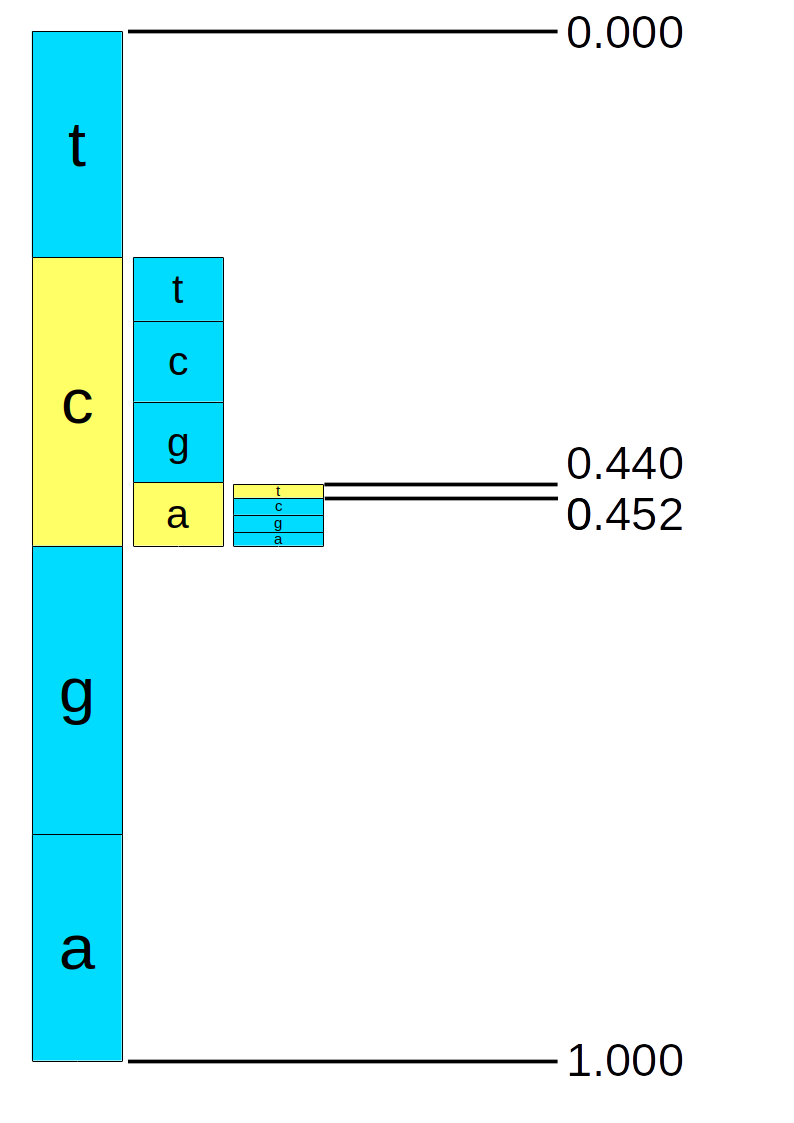
\includegraphics[height=250pt, keepaspectratio=true]{img/range_code.png}

Decoding is simply the reverse of this.  In the above picture we can see that 0.45 would read off `c', `a' and `t' by repeatedly comparing the symbol ranges to the current range and using those to identify the symbol and produce a new range.

\begin{threeparttable}[t]
\begin{tabular}{rrrr}
\hline
\textbf{Range low} & \textbf{Range high} & \textbf{Fraction into range} & \textbf{Symbol}\\
\hline
0.000 & 1.000 & 0.450 & c\\
0.200 & 0.500 & 0.833\tnote{\textbf{a}} & a\\
0.440\tnote{\textbf{b}} & 0.500 & 0.167 & t\\
\hline
\end{tabular}
\begin{tablenotes}
\item{\textbf{a.}} 0.45 into range 0.2 to 0.5: $(0.45-0.2)/(0.5-0.2) = 0.833$.
This falls within the 0.8 to 1.0 symbol range for `a'.
\item{\textbf{b.}} `a' symbol range 0.8 to 1.0 applied to range 0.2 to 0.5:  $0.2+0.8\times(0.5-0.2) = 0.44$ and $0.2+1.0\times(0.5-0.2) = 0.5$.
\end{tablenotes}
\end{threeparttable}

Note: The above example not how the actual implementation works\footnote{This implementation was designed by Eugene Shelwein, based on Michael Schindler's earlier work.}.
For efficiency, we use integer values having a starting range of 0 to $2^{32}-1$.
We write out the top 8-bits of the range when low and high become the same value.
Special care needs to be taken to handle small values are are numerically close but stradding a top byte value, such as 0x37ffba20 to 0x38000034.
The decoder does not need to do anything special here, but the encoder must track the number of 0xff or 0x00 values to emit in order to avoid needing arbitrary precision integers.

Pseudocode for the range codec decoding follows.
This implementation uses code (next few bytes in the current bit-stream) and range instead of low and high, both 32-bit unsigned integers.
This specification focuses on decoding, but given the additional complexity of the precision overflows in encoder we describe this implementation too.

\textsc{RangeDecodeCreate} initialises the range coder, reading the first bytes of the compressed data stream.

\begin{algorithmic}[1]
\Function{RangeDecodeCreate}{}
  \settowidth{\maxwidth}{range\ }
  %\State \algalign{low}{\gets} $0$\Comment{32-bit unsigned}
  \State \algalign{range}{\gets} $2^{32}-1$\Comment{Maximum 32-bit unsigned value}
  \State \algalign{code}{\gets} $0$\Comment{32-bit unsigned}
  \For{$i \gets 0$ to $4$}
    \State $code \gets (code \shiftl 8) + $\Call{ReadUint8}{}
  \EndFor
  \State $code \gets code \bitand 2^{32}-1$
  \State \Return this range coder ($range$, $code$)
\EndFunction
\end{algorithmic}

Decoding each symbol is in two parts; getting the current frequency and updating the range.

\begin{algorithmic}[1]
\Function{RangeGetFreq}{$tot\_freq$}
  \State $range \gets range \bdiv tot\_freq$
  \State \Return $code \bdiv range$
\EndFunction
\end{algorithmic}

\begin{algorithmic}[1]
\Procedure{RangeDecode}{$sym\_low, sym\_freq, tot\_freq$}
  \settowidth{\maxwidth}{range\ }
  \State \algalign{code}{\gets} $code - sym\_low \times range$
  \State \algalign{range}{\gets} $range \times sym\_freq$

  \While{$range < 2^{24}$} \Comment{Renormalise}
    \settowidth{\maxwidth}{range\ }
    \State \algalign{range}{\gets} $range \shiftl 8$
    \State \algalign{code}{\gets} $(code\shiftl8) + $\Call{ReadUint8}{}
  \EndWhile
\EndProcedure
\end{algorithmic}

As mentioned above, the encoder is more complex as it cannot shift out the top byte until it has determined the value.
This can take a considerable while if our current low / high (low + range) are very close but span a byte boundary, such as 0x37ffba20 to 0x38000034, where ultimately we will later emit either 0x37 or 0x38.
To handle this case, when the range gets too small but the top bytes still differ, the encoder caches the top byte of low (0x37) and keeps track of how many 0xff or 0x00 values will need to be written out once we finally observe which value the range has shrunk to.

The \textsc{RangeEncode} function is a straight forward reversal of the \textsc{RangeDecode}, with the exception of the special code for shifting the top byte out of the $low$ variable.

\begin{algorithmic}[1]
\Procedure{RangeEncode}{$sym\_low, sym\_freq, tot\_freq$}
  \settowidth{\maxwidth}{old\_low\ }
  \State \algalign{old\_low}{\gets} $low$
  \State \algalign{range}{\gets} $range \bdiv tot\_freq$
  \State \algalign{low}{\gets} $low + sym\_low \times range$
  \State \algalign{range}{\gets} $range \times sym\_freq$

  \Statex
  \If{low < old\_low}
    \State $carry \gets 1$ \Comment{overflow}
  \EndIf
  \While{$range < 2^{24}$} \Comment{Renormalise}
    \settowidth{\maxwidth}{range\ }
    \State \algalign{range}{\gets} $range \shiftl 8$
    \State \Call{RangeShiftLow}{}
  \EndWhile
\EndProcedure
\end{algorithmic}

\textsc{RangeShiftLow} is the main heart of the encoder renormalisation.
It tracks the total number of extra bytes to emit and $carry$ indicates whether they are a string of 0xFF or 0x00 values.

\begin{algorithmic}[1]
\Procedure{RangeShiftLow}{}
  \If{$low < $ 0xff000000 $\logor carry \ne 0$}
    \If{$carry = 0$}
      \State \Call{WriteByte}{$cache$} \Comment{top byte $cache$ plus FFs}
      \While{$FFnum > 0$}
        \State \Call{WriteByte}{0xff}
        \State $FFnum \gets FFnum - 1$
      \EndWhile
    \Else
      \State \Call{WriteByte}{$cache + 1$} \Comment{top byte $cache+1$ plus 00s}
      \While{$FFnum > 0$}
        \State \Call{WriteByte}{0}
        \State $FFnum \gets FFnum - 1$
      \EndWhile
    \EndIf
    \State $cache \gets low \shiftr 24$ \Comment{Copy of top byte ready for next flush}
    \State $carry \gets 0$
  \Else
    \State $FFnum \gets FFnum + 1$
  \EndIf
  \Statex
  \State $low \gets low \shiftl 8$
\EndProcedure
\end{algorithmic}

For completeness, the Encoder initialisation and finish functions are below.

\begin{algorithmic}[1]
\Procedure{RangeEncodeStart}{}
  \settowidth{\maxwidth}{FFnum\ }
  \State \algalign{low}{\gets} $0$
  \State \algalign{range}{\gets} $2^{32}-1$
  \State \algalign{FFnum}{\gets} $0$
  \State \algalign{carry}{\gets} $0$
  \State \algalign{cache}{\gets} $0$
\EndProcedure
\end{algorithmic}

\begin{algorithmic}[1]
\Procedure{RangeEncodeEnd}{}
  \For{$i \gets 0$ to $4$} \Comment{Flush any residual state in $low$}
    \State \Call{RangeShiftLow}{}
  \EndFor
\EndProcedure
\end{algorithmic}


\subsection{Statistical Modelling}

The probabilities passed to the range coder may be fixed for all scenarios (as we had in the ``cat'' example), or they may be adaptive and context aware.
For example the letter `u' occurs around 3\% of time in English text, but if the previous letter was `q' it is close to 100\% and if the previous letter was `u' it is close to 0\%.
Using the previous letter is known as an Order-1 entropy encoder, but the context can be anything.
We can also adaptively adjust our probabilities as we encode or
decode, learning the likelihoods and thus avoiding needing to store
frequency tables in the data stream covering all possible contexts.

To do this we use a statistical model, containing an array of symbols $S$ and their frequencies $F$.
The sum of these frequences must be less than $2^{16}-32$.
When they get too high, they are renormalised by approximately halving the frequencies (ensuring none drop to zero).

Typically an array of models are used where the array index represents the current context.

To encode any symbol the entropy encoder needs to know the frequency of the symbol to encode, the cumulative frequencies of all symbols prior to this symbol, and the total of all frequencies.
For decoding a cumulative frequency is obtained given the frequency total and the appropriate symbol is found matching this frequency.
Symbol frequencies are updated after each encode or decode call and the symbols are kept in order of most-frequent symbol first in order to  reduce the overhead of scanning through the cumulative frequencies.

\textsc{ModelCreate} initialises a model by setting every symbol to have a frequency of 1.
(At no point do we permit any symbol to have zero frequency.)

\begin{algorithmic}[1]
\Function{ModelCreate}{$num\_sym$}
  \State $total\_freq \gets num\_sym$
  \State $max\_sym \gets num\_sym-1$
  \For{$i \gets 0$ to $max\_sym$}
    \State $S_i \gets i$
    \State $F_i \gets 1$
  \EndFor
  \State \Return this model ($total\_freq$, $max\_sym$, $S$, $F$)
\EndFunction
\end{algorithmic}

\textsc{ModelDecode} is called once for each decoded symbol.
It returns the next symbol and updates the model frequencies automatically.

\begin{algorithmic}[1]
\Function{ModelDecode}{rc}
  \State $freq \gets$ $rc.$\Call{RangeGetFrequency}{$total\_freq$}
  \State $x \gets 0$
  \State $acc \gets 0$
  \While{$acc + F_x \le freq$}
    \State $acc \gets acc + F_x$
    \State $x \gets x+1$
  \EndWhile
  \State $rc.$\Call{RangeDecode}{$acc,\ F_x,\ total\_freq$}
  \State $F_x \gets F_x + 16$ \Comment{Update model frequencies}
  \State $total\_freq \gets total\_freq + 16$
  \If{$total\_freq > 2^{16}-17$}
    \State \Call{ModelRenormalise}{}
  \EndIf
  \State $sym \gets S_x$
  \If{$x > 0 \logand F_x > F_{x-1}$}
    \State \Call{Swap}{$F_x$, $F_{x-1}$}
    \State \Call{Swap}{$S_x$, $S_{x-1}$}
  \EndIf
  \State \Return $sym$
\EndFunction
\end{algorithmic}

\textsc{ModelRenormalise} is called whenever the total frequencies get too high.
The frequencies are halved, taking sure to avoid any zero frequencies being created.

\begin{algorithmic}[1]
\Procedure{ModelRenormalise}{}
  \State $total\_freq \gets 0$
  \For{$i \gets 0$ to $max\_sym$}
    \State $F_i \gets F_i - (F_i \bdiv 2)$
    \State $total\_freq \gets total\_freq + F_i$
  \EndFor
\EndProcedure
\end{algorithmic}

\subsection{Order-0 and Order-1 Encoding}

We can combine the model defined above and the range coder to provide a simple function to perform Order-0 entropy decoder.

\begin{algorithmic}[1]
\Function{DecodeOrder0}{$len$}
  \State $max\_sym \gets $\Call{ReadUint8}{}
  \If{$max\_sym = 0$}
    \State $max\_sym \gets 256$
  \EndIf
  \State $model\_lit \gets $\Call{ModelCreate}{$max\_sym$}
  \Statex
  \State $rc \gets $\Call{RangeDecodeCreate}{}
  \For{$i \gets 0$ to $len-1$}
    \State $out_i \gets model\_lit.$\Call{ModelDecode}{$rc$}
  \EndFor
  \State \Return $out$
\EndFunction
\end{algorithmic}

The Order-1 variant simply uses an array of models and selects the appropriate model based on the previous value encoded or decoded.
This array index is our ``context''.

\begin{algorithmic}[1]
\Function{DecodeOrder1}{$len$}
  \State $max\_sym \gets $\Call{ReadUint8}{}
  \If{$max\_sym = 0$}
    \State $max\_sym \gets 256$
  \EndIf
  \For{$i \gets 0$ to $max\_sym-1$}
    \State $model\_lit_i \gets $\Call{ModelCreate}{$max\_sym$}
  \EndFor
  \Statex
  \State $rc \gets $\Call{RangeDecodeCreate}{}
  \State $last \gets 0$
  \For{$i \gets 0$ to $len-1$}
    \State $out_i \gets model\_lit_{last}.$\Call{ModelDecode}{$rc$}
    \State $last \gets out_i$
  \EndFor
  \State \Return $out$
\EndFunction
\end{algorithmic}

\subsection{RLE with Order-0 and Order-1 Encoding}

The \textsc{DecodeOrder0} and \textsc{DecodeOrder1} codecs can be expanded to include a count of how many runs of each symbol should be decoded.
Both order 0 and order 1 variants are possible.

After the symbol is decoded, the run length must be decoded to
indicate how many \emph{extra} copies of this symbol occur.  Long runs
are broken into a series of lengths of no more than 3.  If length 3
is decoded it indicates we must decode an additional length and add to
the current one.  The context used for the run length model is the
symbol itself for the initial run, 256 for the first continuation run
(if $\ge 4$) and 257 for any further continuation runs.  Thus encoding
10 `A' characters would first store symbol `A' followed by run length
3 (with context `A'), length 3 (context 256), length 3 (context
257), and length 1 (context 258).

For example, if we have the string ``RRRRUNN'' we will decode
symbol `R' run 3, symbol `U' run 0, symbol `N' run 1.

\begin{algorithmic}[1]
\Function{DecodeRLE0}{$len$}
  \State $max\_sym \gets $\Call{ReadUint8}{}
  \If{$max\_sym = 0$}
    \State $max\_sym \gets 256$
  \EndIf
  \State $model\_lit \gets $\Call{ModelCreate}{$max\_sym$}

  \For{$i \gets 0$ to $257$}
    \State $model\_run_i \gets $\Call{ModelCreate}{$4$}
  \EndFor
  \Statex
  \State $rc \gets $\Call{RangeDecodeCreate}{}
  \State $i \gets 0$
  \While{$i < len$}
    \State $out_i \gets model\_lit.$\Call{ModelDecode}{$rc$}
    \State $part \gets model\_run_{out_i}.$\Call{ModelDecode}{$rc$}
    \State $run \gets part$
    \State $rctx \gets 256$
    \While{$part = 3$}
      \State $part \gets model\_run_{rctx}.$\Call{ModelDecode}{$rc$}
      \State $rctx \gets 257$
      \State $run \gets run + part$
    \EndWhile
    \For{$j \gets 1$ to $run$}
      \State $out_{i+j} \gets out_i$
    \EndFor
    \State $i \gets run+1$
  \EndWhile
  \State \Return $out$
\EndFunction
\end{algorithmic}

The order-1 run length variant is identical to order-0 except the
previous symbol is used as the context for the next literal.  The
context for the run length does not change.

\begin{algorithmic}[1]
\Function{DecodeRLE1}{$len$}
  \State $max\_sym \gets $\Call{ReadUint8}{}
  \If{$max\_sym = 0$}
    \State $max\_sym \gets 256$
  \EndIf
  \For{$i \gets 0$ to $max\_sym-1$}
    \State $model\_lit_i \gets $\Call{ModelCreate}{$max\_sym$}
  \EndFor
  \For{$i \gets 0$ to $257$}
    \State $model\_run_i \gets $\Call{ModelCreate}{$4$}
  \EndFor
  \Statex
  \State $rc \gets $\Call{RangeDecodeCreate}{}
  \State $last \gets 0$
  \State $i \gets 0$
  \While{$i < len$}
    \State $out_i \gets model\_lit_{last}.$\Call{ModelDecode}{$rc$}
    \State $last \gets out_i$
    \State $part \gets model\_run_{last}.$\Call{ModelDecode}{$rc$}
    \State $run \gets part$
    \State $rctx \gets 256$
    \While{$part = 3$}
      \State $part \gets model\_run_{rctx}.$\Call{ModelDecode}{$rc$}
      \State $rctx \gets 257$
      \State $run \gets run + part$
    \EndWhile
    \For{$j \gets 1$ to $run$}
      \State $out_{i+j} \gets last$
    \EndFor
    \State $i \gets run+1$
  \EndWhile
  \State \Return $out$
\EndFunction
\end{algorithmic}

%\subsection{General Purpose Entropy Encoder}

We wrap up the Order-0 and 1 entropy encoder, both with and without run length encoding, into a data stream that specifies the type of encoded data and also permits a number of additional transformations to be applied.
These transformations support bit packing (for example a data block with only 4 distinct values can be packed with 4 values per byte), no-op for tiny data blocks where entropy encoding would grow the data and N-way interleaving of the 8-bit components of a 32-bit value.

\begin{table}[h]
\centering
\begin{tabular}{|r|r|r|r|p{9cm}|l|}
\hline
\multicolumn{2}{|r|}{\textbf{Bits} } & \textbf{Type}  & \textbf{Name} & \multicolumn{2}{p{9cm}|}{\textbf{Description}} \\
\hline
\multicolumn{2}{|r|}{8} & uint8 & $flag$ & \multicolumn{2}{p{9cm}|}{Data format bit field}\\
\cline{1-6}

\multicolumn{6}{|l|}{}\\[-0.3em]
\multicolumn{6}{|l|}{\textit{Unless \textsc{NoSize} flag is set:} } \\
\cline{2-5}
& ? & uint7 & ulen & Uncompressed length & \\
\cline{2-5}

\multicolumn{6}{|l|}{}\\[-0.3em]
\multicolumn{6}{|l|}{\textit{If \textsc{Stripe} flag is set:} } \\
\cline{2-5}
& ? & uint8 & N & Number of sub-streams & \\
& ? & uint7[] & clen[] & N copies of compressed sub-block length & \\
& ? & uint8[] & cdata[] & N copies of Compressed data sub-block (recurse) & \\
\cline{2-5}

\multicolumn{6}{|l|}{}\\[-0.7em]
\multicolumn{6}{|l|}{\textit{If \textsc{Cat} flag is set (and \textsc{Stripe} flag is unset):} } \\
\cline{2-5}
& ? & uint8[] & udata & Uncompressed data stream & \\
\cline{2-5}

\multicolumn{6}{|l|}{}\\[-0.7em]
\multicolumn{6}{|l|}{\textit{If \textsc{Pack} flag is set (and neither \textsc{Stripe} or \textsc{Cat} flags are set):} } \\
\cline{2-5}
& ? & uint8[] & pack\_meta & Pack lookup table & \\
\cline{2-5}

\multicolumn{6}{|l|}{}\\[-0.7em]
\multicolumn{6}{|l|}{\textit{If neither \textsc{Stripe} or \textsc{Cat} flags are set:} } \\
\cline{2-5}
& ? & uint8[] & cdata & Entropy encoded data stream (see \textsc{Order} / \textsc{RLE} / \textsc{Ext} flags) & \\
\cline{2-5}
\multicolumn{6}{|l|}{}\\
\hline
\end{tabular}
\end{table}

The first byte of our generalised data stream is a bit-flag detailing the type of transformations and entropy encoders to be combined, followed by optional meta-data, followed by the actual compressed data stream.
The bit-flags are defined below, but note not all combinations are permitted.

\begin{threeparttable}[t]
\begin{tabular}{llll}
\hline
\textbf{Bit AND value} & \textbf{Code} & \textbf{Description} \\
\hline
1 & \textsc{Order}\tnote{\textbf{a}} & Order-0 or Order-1 entropy coding. \\
2 & reserved & Reserved (for possible order-2/3)\\
4 & \textsc{Ext} & ``External'' compression via bzip2\\
8 & \textsc{Stripe}\tnote{\textbf{b}} & N-way interleaving of byte streams.\\
16 & \textsc{NoSize} & original size is not recorded (used by \textsc{Stripe})\\
32 & \textsc{Cat}\tnote{\textbf{b}} & Data is uncompressed\\
64 & \textsc{RLE}\tnote{\textbf{a}} & Run length encoding, with runs and literals encoded separately\\
128 & \textsc{Pack} & Pack 2, 4, 8 or infinite symbols per byte.\\
\hline
\end{tabular}
\begin{tablenotes}
\item{\textbf{a.}} Has no effect when \textsc{Ext} flag is set.
\item{\textbf{b.}} Not to be used in conjunction with other flags
  except \textsc{Pack} and \textsc{NoSize}.
\end{tablenotes}
\end{threeparttable}

Of these \textsc{Stripe} is the most complex.
As with the rANS4x16 encoder, the data is rearranged such that every
$N^{th}$ byte is adjacent in a single block producing N distinct sub-blocks.
Each of the N streams is then itself compressed using this compression format.

For example an input block of small unsigned 32-bit little-endian numbers may use RLE for the first three streams as they are mostly zero, and a non-RLE Order-0 entropy encoder of the last stream.
Normally our data format will include the decoded size, but with \textsc{Stripe} we can omit this from the internal compressed streams as we know their size will be a computable fraction of the combined data.

The data layout differs for each of these bit types, as described below in the \textsc{ArithDecode} function.
Some of these can be used in combination, so the order needs to be observed.
The Pack format has additional meta data.
This is decoded first, before entropy decoding and finally expanding thespecified pack transformation after decompression.
For example value 193 is indicates a byte stream should be decoded with an RLE aware order-1 entropy encoder and then unpacked.

\begin{algorithmic}[1]
\Function{ArithDecode}{$len$}
  \State $flags \gets $\Call{ReadUint8}{}
  \If{$flags \bitand$ \textsc{NoSize} $\ne 0$}
    \State $len \gets$\Call{ReadUint7}{}
  \EndIf
  \If{$flags \bitand$ \textsc{Stripe}}
    \State $data \gets $\Call{DecodeSTRIPE}{$len$}
    \State \Return $data$
  \EndIf{}
  \If{$flags \bitand$ \textsc{Pack}}
    \State $pack\_len \gets len$
    \State $(P,\ nsym,\ len) \gets $\Call{DecodePackMeta}{}
  \EndIf
  \Statex \Comment{Entropy Decoding}
  \If{$flags \bitand$ \textsc{Cat}}
    \State $data \gets $\Call{ReadData}{$len$}
  \ElsIf{$flags \bitand$ \textsc{Ext}}
    \State $data \gets $\Call{DecodeEXT}{$len$}
  \ElsIf{$flags \bitand$ \textsc{RLE}}
    \If{$flags \bitand$ \textsc{Order}}
      \State $data \gets $\Call{DecodeRLE1}{$len$}
    \Else
      \State $data \gets $\Call{DecodeRLE0}{$len$}
    \EndIf
  \Else
    \If{$flags \bitand$ \textsc{Order}}
      \State $data \gets $\Call{DecodeOrder1}{$len$}
    \Else
      \State $data \gets $\Call{DecodeOrder0}{$len$}
    \EndIf
  \EndIf
  \Statex \Comment{Apply data transformations}
  \If{$flags \bitand$ \textsc{Pack}}
    \State $data \gets $\Call{DecodePack}{$data$, $P$, $nsym$, $pack\_len$}
  \EndIf
  \State \Return $data$
  \EndFunction
\end{algorithmic}

The specifics of each sub-format are described below, in the order (minus meta-data specific shuffling) they are applied.

\begin{itemize}
\item{\textbf{\textsc{Stripe}}:}
The byte stream consists of a 7-bit encoded uncompressed length and a
byte holding the number of substreams $N$, and their 7-bit encoded
compressed data streams lengths.  This is then followed by the
substreams themselves, each of which is a valid $cdata$ stream as
defined above, hence this offers a recursive mechanism as each
substream has its own format byte.

The total uncompressed byte stream is then an interleaving of one byte
in turn from each of the N substreams (in order of 1st to Nth).  Thus
an array of 32-bit unsigned integers could be unpacked using
\textsc{Stripe} to compress each of the 4 8-bit components together with
their own algorithm.

\begin{algorithmic}[1]
\Function{RansDecodeStripe}{$len$}
  \State $N \gets $\Call{ReadUint8}{}
  \For{$j \gets 0$ to $N$} \Comment{Fetch N compressed lengths}
    \State $clen_j \gets $\Call{ReadUint7}{}
  \EndFor
  \Statex
  \For{$j \gets 0$ to $N$} \Comment{Decode N streams}
    \State $ulen_j \gets (len \bdiv N) + ((len \bmod N) > j)$
\Comment{$(x > y)$ expression being 1 if true, 0 if false}
    \State $T_j \gets $\Call{ArithDecode}{$ulen_j$}
  \EndFor
  \Statex
%  \For{$i \gets 0$ to $len - 1$} \Comment{Interleave}
%    \State $out_i \gets T_{(i \bmod N),\ (i \bdiv N)}$
%  \EndFor
  \For{$j \gets 0$ to $N - 1$} \Comment{Interleave}
    \For{$i \gets 0$ to $ulen_j - 1$}
      \State $out_{i \times N + j} \gets T_{j,i}$
    \EndFor
  \EndFor
  \State \Return $out$
\EndFunction
\end{algorithmic}

\item{\textbf{\textsc{NoSize}}:}
Do not store the size of the uncompressed data stream.
This information is not required when the data stream is one of the four sub-streams in the \textsc{Stripe} format.

\item{\textbf{\textsc{Cat}}:}
If present, all other bit flags should be nul, with the possible
exception of \textsc{NoSize} or \textsc{Pack}.

The uncompressed data stream is the same as the compressed stream.
This is useful for very short data where the overheads of compressing are too high.

\item{\textbf{\textsc{Order}}:}
Bit field defining order-0 (unset) or order-1 (set) entropy encoding, as described above by the \textsc{DecodeOrder0} and \textsc{DecodeOrder1} functions.

\item{\textbf{\textsc{RLE}}:}
Bit field defining whether the Order-0 and Order-1 encoding should also use a run-length.
When set, the \textsc{DecodeRLE0} and \textsc{DecodeRLE1} functions will be used instead of \textsc{DecodeOrder0} and \textsc{DecodeOrder1}.

\item{\textbf{\textsc{Ext}}:}
Instead of using the adaptive arithmetic coder for decompression (with or without RLE), this uses an compression codec defined in an ``external'' library.
Currently the only supported such codec is Bzip2.
In future more may be added, so the magic number \emph{must} be validated to check the codec being used.

Given bzip2 is already supported elsewhere in CRAM, the purpose of adding it here is to permit bzip2 compression after \textsc{Pack} and \textsc{Stripe} transformations.
This may be tidied up in later CRAM releases to clarify the separation between compression codecs and data transforms, but that requires more major restructuring so for compatibility with v3.0 these have been placed into this single codec.

\begin{algorithmic}[1]
\Function{DecodeExt}{$len$}
  \If{Bzip2 magic number is present}
    \State \Return \Call{DecodeBzip2}{$len$}
  \Else
    \State Error
  \EndIf
\EndFunction
\end{algorithmic}

\item{\textbf{\textsc{Pack}}:}
Data containing only 1, 2, 4 or 16 distinct values can have multiple
values packed into a single byte (infinite, 8, 4 or 2).  The distinct
symbol values do not need to be adjacent as a mapping table $P$
converts mapped value $x$ to original symbol $P_x$.

The packed format is split into uncompressed meta-data (below) and the
compressed packed data as described in the rANS 4x16 bit-packing section.
The same \textsc{DecodePackMeta} and \textsc{DecodePack} functions are used.

\end{itemize}

\section{Name tokenisation codec}

Sequence names (identifiers) typically follow a structured pattern and compression based on columns within those structures usually leads to smaller sizes.
The sequence name (identifier) tokenisation relies heavily on the General Purpose Entropy Encoder described above.

As an example, take a series of names:

\begin{verbatim}
I17_08765:2:123:61541:01763#9
I17_08765:2:123:1636:08611#9
I17_08765:2:124:45613:16161#9
\end{verbatim}

We may wish to tokenise each of these into 7 tokens, e.g.
``I17\_08765:2:'', ``123'', ``:'', ``61541'', ``:'', ``01763''and
``\#9''. Some of these are multi-byte strings, some single characters,
and some numeric, possibily with a leading zero.  We also observe some
regularly have values that match the previous line (the initial prefix
string, colons, ``\#9'') while others are numerically very close to the
value in the previous line (124 vs 123).

The name tokeniser compares each name against a previous name (which
is not necessarily the one immediately prior) and encodes this name
either as a series of differences to the previous name or marking it
as an exact duplicate.  A maximum of 128 tokens are permitted within
any single read name.

Token IDs (types) are listed below.

\begin{tabular}{lllp{10cm}}
\hline
\textbf{ID} & \textbf{Type} & \textbf{Value} & \textbf{Description}\\
\hline
 0 & TYPE    & Type    & Used to determine the type of token at a given position. \\
\hline
 5 & DUP     & Integer (distance) & The entire name is a duplicate of an earlier one.  Used in position 0 only.\\
 6 & DIFF    & Integer (distance) & The entire name is differs to earlier ones.  Used in position 0 only.\\
\hline
 1 & STRING  & String  & A nul-terminated string of characters \\
 2 & CHAR    & Byte    & A single character \\
 7 & DIGITS  & $0 \le$ Int $< 2^{32}$ & A numerical value, not containing a leadng zero \\
 3 & DIGITS0 & $0 \le$ Int $< 2^{32}$ & A numerical value possibly starting in leading zeros \\
 4 & DZLEN   & Int length & Length of associated DIGITS0 token.\\
 8 & DELTA  & $0 \le$ Int $< 256$   & A numeric value being stored as the difference to the numeric value of this token on the previous name. \\
 9 & DELTA0 & $0 \le$ Int $< 256$ & As DELTA, but for numeric values starting with leading zeros \\
10 & MATCH   & (none) & This token is identical type and value to the same position in the previous name (NB: not permitted for DELTA/DELTA0)\\
11 & NOP & (none) & Does nothing\\
12 & END     & (none) & Marks end of name\\
\hline
\end{tabular}

The tokens and values are stored in a 2D array of byte streams,
$B_{pos,type}$, where pos 0 is reserved for name meta-data (whether it
is a duplicate name) and pos 1 onwards is for the first, second and
later tokens.  $Type$ is one of the token types listed above,
corresponding to the type of data being stored.  Some token types may
also have associated values.  $B_{pos,\texttt{TYPE}}$ ($type$) holds the token
type itself and that is then used to retrieve any associated
value(s) if appropriate from $B_{pos,type}$.  Thus multiple types at the same token
position will have their values encoded in distinct data streams,
e.g. if position 5 is of type either DIGITS or DELTA then data streams
will exist for $B_{5,\texttt{TYPE}}$, $B_{5,\texttt{DIGITS}}$ and $B_{5, \texttt{DELTA}}$.
Decoding per name continues until a token of type END is observed.

More detail on the token types is given below.

\begin{itemize}
\item{\textbf{TYPE}:}
This is the first token fetched at each token position.  It holds the
type of the token at this position, which in turn may then require
retrieval from type-specific data streams at this position.

For position 0, the TYPE field indicates whether this record is an
exact duplicate of a prior read name or has been encoded as a delta to
an earlier one.

\item{\textbf{DUP}, \textbf{DIFF}:}
These types are fetched for position 0, at the start of each new
identifier.  The value is an integer value describing how many reads
before this (with 1 being the immediately previous name) we are
comparing against.  When we refer to ``previous name'' below, we
always mean the one indicated by the DIFF field and not the one
immediately prior to the current name.

The first record will have a DIFF of zero and no delta or match
operations are permitted.

\item{\textbf{STRING}:}
We fetch one byte at a time from the value byte stream, appending to the
name buffer until the byte retrieved is zero.  The zero byte is not
stored in the name buffer.
For purposes of token type MATCH, a match is defined as entirely
matching the string including its length.

\item{\textbf{CHAR}:}
Fetch one single byte from the value byte stream and append to the name buffer.

\item{\textbf{DIGITS}:}
Fetch 4 bytes from the value byte stream and intrepret these as a little
endian unsigned integer.  This is appended to the name buffer as
string of base-10 digits, most significant digit first.  Larger
values may be represented, but will require multiple DIGITS tokens.
Negative values may be encoded by treating the minus sign as a CHAR or
STRING and storing the absolute value.

\item{\textbf{DIGITS0}, \textbf{DZLEN}:}
This fetches the 4 byte value from $B_{pos,DIGITS0}$ and a 1 byte
length from $B_{pos,DZLEN}$.  As per DIGITS, the value is intrepreted as a
little endian unsigned integer.  The length indicates the total
size of the numeric value when displayed in base 10 which must be
greater than $\log_{10}(value)$ with any remaining length indicating
the number of leading zeros.  For example if DIGITS0 value is 123 and
DZLEN length is 5 the string ``00123'' must be appended to the name.

For purposes of the MATCH type, both value and length must match.

\item{\textbf{DELTA}:}
Fetch a 1 byte value and add this to the DIGITS value from the
previous name.
The token in the prior name must be of type DIGITS or DELTA.

MATCH is not supported for this type.

\item{\textbf{DELTA0}:}
As per DELTA, but the 1 byte value retrieved is added to the DIGITS0
value in the previous name.  No DZLEN value is retrieved, with the
length from the previous name being used instead.
The token in the prior name must be of type DIGITS0 or DELTA0.

MATCH is not supported for this type.

\item{\textbf{MATCH}:}
This token matches the token at the same position in the previous
name.  (The previous name is permitted to also have a MATCH token at
this position, in which case it recurses to its previous name.)

MATCH is only valid when the token being matched against is CHAR,
STRING, DIGITS, DIGITS0 or MATCH.  (I.e. matching a numeric delta will not
repeat the delta increment.)

No value is needed for MATCH tokens.

\item{\textbf{NOP}:}
This token type does nothing.
The purpose of this is simply to permit skipping tokens in order to
keep token numbers in sync, such as when processing ``10'' vs ``-10''
with the latter needing an additional ``-'' token.

\item{\textbf{END}:}
Marks the end of the name.  A nul byte is added to the name output
buffer.  No value is needed for END tokens.
\end{itemize}

Decoding needs some simple functions to read successive bytes from our token byte streams, as 8-bit characters or unsigned integers, as 32-bit unsigned integers and nul-terminated strings.  We reuse the \textsc{ReadUint32} and related functions with the byte array specified as input.

\begin{algorithmic}[1]
\Statex
\Statex \textit{(Convert an integer to a string form in base-10 digits, at least $len$ bytes long with leading zeros)}
\Function{LeftPadNumber}{$val,\ len$}
  \State $str \gets val$ \Comment{Implicit language-specific Integer to String conversion}
  \While{\Call{Length}{$str$} < $len$}
    \State $str \gets$ `$0$' $ \concat str$
  \EndWhile
  \State \Return $str$
\EndFunction
\end{algorithmic}

For the main name decoding loop, we use a single dimensional array of
names decoded so far, $N$, and a two dimensional array of their tokens
$T$ (indexed by name number $n$ and token position $t$ within that
name).  We define a function to decode the $n^{th}$ name ($N_n$) using
a previous $m^{th}$ name ($N_m$).  The tokens $T$ are used in
\texttt{MATCH} and \texttt{DELTA} token types to copy data from when
constructing the name.

Now we have the basic primitives for pulling from the $B$ byte
streams, decoding the $n^{th}$ individual name is as
follows\footnote{For simplicity of algorithm description, we take a
  flexible approach as to whether we read/write $T$ in numeric or
  string form.  For example a \texttt{DELTA} token will fetch the
  previous token as a string, interpret it as a numeric value, add to
  it, and then write it back as a string.  Practical implementations
  may wish to separate out T into distinct integer and string
  arrays.}:


\begin{algorithmic}[1]
\Statex
\Statex \textit{(Decodes the $n^{th}$ name, returning $N_n$ and updating globals $N_n$ and $T_n$)}
\Function{DecodeSingleName}{$n$}
  \State $type \gets$ \Call{ReadUint8}{$B_{0,\textit{TYPE}}$}
  \State $dist \gets$ \Call{ReadUint32}{$B_{0,type}$}
  \State $m \gets n-dist$
  \If{$type = $ \texttt{DUP}}
    \State $N_n \gets N_m$
    \State $T_n \gets T_m$ \Comment{Copy for all $T_{n,*}$}
    \State \Return $N_n$
  \EndIf
  \Statex
  \State $t \gets 1$ \Comment{Token number $t$}
  \Repeat
    \State $type \gets$ \Call{ReadUint8}{$B_{t,\texttt{TYPE}}$}
    \If{$type = $ \texttt{CHAR}}
      \State $T_{n,t} \gets$ \Call{ReadChar}{$B_{t,\texttt{CHAR}}$}
    \ElsIf{$type = $ \texttt{STRING}}
      \State $T_{n,t} \gets$ \Call{ReadString}{$B_{t,\texttt{STRING}}$}
    \ElsIf{$type = $ \texttt{DIGITS}}
      \State $T_{n,t} \gets$ \Call{ReadUint32}{$B_{t,\texttt{DIGITS}}$}
    \ElsIf{$type = $ \texttt{DIGITS0}}
      \State $d \gets$ \Call{ReadUnt32}{$B_{t,\texttt{DIGITS0}}$}
      \State $l \gets$ \Call{ReadUint8}{$B_{t,\texttt{DZLEN}}$}
      \State $T_{n,t} \gets$ \Call{LeftPadNumber}{$d,\ l$}
    \ElsIf{$type = $ \texttt{DELTA}}
      \State $T_{n,t} \gets T_{m,t} + $ \Call{ReadUint8}{$B_{t,\texttt{DELTA}}$}
    \ElsIf{$type = $ \texttt{DELTA0}}
      \State $d \gets T_{m,t} + $ \Call{ReadUint8}{$B_{t,\texttt{DELTA0}}$}
      \State $l \gets$ \Call{Length}{$T_{m,t}$} \Comment{String length including leading zeros}
      \State $T_{n,t} \gets$ \Call{LeftPadNumber}{$d,\ l$}
    \ElsIf{$type = $ \texttt{MATCH}}
      \State $T_{n,t} \gets T_{m,t}$
    \Else
      \State $T_{n,t} \gets$\ `'
    \EndIf
    \State $N_n \gets N_n \concat T_{n,t}$
    \State $t \gets t+1$
  \Until{$type = $ \texttt{END}}
  \State \Return $N_n$
\EndFunction
\end{algorithmic}

Given a complex name with both position and type specific values, this
can lead to many separate data streams.  The name tokeniser codec is
a format within a format, as the multiple byte streams $B_{pos,type}$
are serialised into a single byte stream.

The serialised data stream starts with two unsigned little endiand 32-bit
integers holding the total size of uncompressed name buffer and the
number of read names.  This is followed the array elements
themselves.

Token types, $ttype$ holds one of the token ID values listed above
in the list above, plus special values to indicate certain additional
flags.  Bit 6 (64) set indicates that this entire token data stream is a
duplicate of one earlier.  Bit 7 (128) set indicates the token
is the first token at a new position.  This way we only need to store
token types and not token positions.

The total size of the serialised stream needs to be already known, in
order to determine when the token types finish.

\begin{tabular}{|r|r|r|l|l|p{10cm}|}
\hline
\multicolumn{3}{|r|}{\textbf{Bytes}} & \textbf{Type} & \textbf{Name} & \textbf{Description}\\
\hline
\multicolumn{3}{|r|}{4} & uint32 & $uncomp\_length$ & Length of uncompressed name buffer\\
\multicolumn{3}{|r|}{4} & uint32 & $num\_reads$ & Number of read names\\
\multicolumn{3}{|r|}{1} & uint8  & $use\_arith$ & Whether compression is arithmetic (1) or rANS4x16 (0)\\
\hline
\multicolumn{6}{|l|}{\quad\textit{For each token data stream}}\\
\cline{2-6}
& \multicolumn{2}{r|}{1} & uint8 & $ttype$ & Token type code plus flags (64=duplicate, 128=next token position).\\
\cline{2-6}
& \multicolumn{5}{l|}{\textit{If ttype AND 64 (duplicate)}}\\
\cline{3-6}
& & 1 & uint8 & $dup\_pos$  & Duplicate from this token position\\
& & 1 & uint8 & $dup\_type$ & Duplicate from this token type ID\\
\cline{3-6}
& \multicolumn{5}{l|}{\textit{else if not duplicate}}\\
\cline{3-6}
& & ? & i7 & $clen$ & compressed length (7-bit encoding)\\
& & $clen$ & $cdata$ & stream & compressed data stream\\
\hline
\end{tabular}

A few tricks are used to remove some byte streams.  In addition to the explicit marking of duplicate bytes streams, if a byte stream of token types is entirely MATCH apart from the very first value it is discarded.  It is possible to regenerate this during decode by observing the other byte streams.  For example if we have a byte stream $B_{5,DIGITS}$ but no $B_{5,TYPE}$ then we assume the contents of $B_{5,TYPE}$ consist of one DIGITS type followed by as many MATCH types as are needed.

The $cdata$ stream itself is as described in the General Purpose Entropy Encoder section above, with the \textsc{ArithDecode} function.

\begin{algorithmic}[1]
\Statex
\Statex \textit{(Decodes and uncompressed the serialised token byte streams)}
\Function{DecodeTokenByteStreams}{$use\_arith$}
  \State $sz \gets 0$
  \State $t \gets -1$
  \Repeat
    \State $ttype \gets$ \Call{ReadUint8}{}
    \State $tok\_new \gets ttype \bitand 128$
    \State $tok\_dup \gets ttype \bitand 64$
    \State $type \gets ttype \bitand 63$
    \If{$tok\_new \ne 0$}
      \State $t \gets t+1$
      \If{$type \ne \texttt{TYPE}$}
        \State $B_{t,\texttt{TYPE}} \gets (type, \texttt{TOK\_MATCH}, \texttt{TOK\_MATCH}, ...)$\Comment{for $nnames-1$ times}
      \EndIf
    \EndIf
    \Statex
    \If{$tok\_dup \ne 0$}
       \State $dup\_pos \gets$ \Call{ReadUint8}{}
       \State $dup\_type \gets$ \Call{ReadUint8}{}
       \State $B_{t,type} \gets B_{dup\_pos,dup\_type}$
    \Else
      \State $clen \gets$ \Call{ReadUint7}{}
      \State $data \gets$ \Call{ReadData}{$clen$}
      \If{$use\_arith$}
        \State $B_{t,type} \gets$ \Call{ArithDecode}{}
      \Else
        \State $B_{t,type} \gets$ \Call{RansDecode4x16}{}
      \EndIf
    \EndIf
  \Until{\Call{EOF}{}}
  \State \Return $B$
\EndFunction
\end{algorithmic}

\begin{algorithmic}[1]
\Statex
\Statex \textit{(Decodes the $n^{th}$ name, returning $N_n$ and updating $N_n$ and $T_n$)}
\Function{DecodeNames}{}
  \State $ulen \gets$ \Call{ReadUint32}{}
  \State $nnames \gets$ \Call{ReadUint32}{}
  \State $use\_arith \gets$ \Call{ReadUint8}{}
  \State $B \gets$ \Call{DecodeTokenByteStreams}{$use\_arith$}

  \For{$n \gets 0$ to $nnames-1$}
    \State $N_n \gets$ \Call{DecodeSingleName}{$n$}
  \EndFor
  \State \Return $N$
\EndFunction
\end{algorithmic}


\section{FQZComp quality codec}

% Ideas to explore and TODO list:
%
% 1. Move param do_rev to global part.  It's all or nothing
%
% 2. Delta updates immediately on base 0 to base 1.  Maybe delay
%    initialisation so prevq is 1st base qual.
%
% 3. ReadArray pseudocode needs fixing.
%
% 4. Add param sel_offset to subtract from decoded sel.
%    Eg if we have 2 params and max_sel 3 (0..3) then we may want
%    sel 0/1 for 1st param and sel 0/1 (sel_offset 2) for 2nd?
%
% 5. Add len_bytes to param so we don't need Model_len[4] always.
%
% 6. Permit do_term and term_sym to put in newlines (or whatever)
%    after each record. (See 7 below for example)
%
% 7. Add dmap to apply to quals before doing the prevq != q check.
%    Reason is maybe we're not compressing qualities!  Eg SA:Z: tag
%    may be best using dmap , = 1 and everything else = 0.  Then
%    ``chr4,100,5,blah''; becomes delta 000012223456666.  dtab to
%    divide by 2 then allows it to track token number.
%    Each semi-colon separated text is a new record (qlen) and they're
%    joined together with term_sym (6. above).
%
% 8. Consider adding selector as context for model len, rev and dup.
%    This is important on mixed data sets.  Do we want full sel, or
%    quantised stab[sel]?

The FQZComp quality codec uses an adaptive statistical model to
predict the next quality value in a given context (comprised of
previous quality values, position along this sequence, whether the
sequence is the second in a pair, and a running total of number of
times the quality has changed in this sequence).

For each quality value, the models produce probabilities for all
possible next quality values, which are passed into an arithmetic
entropy encoder to encode or decode the actual next quality value.
The models are then updated based on the actual next quality in order
to learn the statistical properties of the quality data stream.  This
step wise update process is identical for both encoding and decoding.

The algorithm is a generalisation on the original fqzcomp program,
described in \textit{Compression of FASTQ and SAM Format Sequencing
  Data} by Bonfield JK, Mahoney MV (2013). PLoS ONE 8(3):
e59190. \url{https://doi.org/10.1371/journal.pone.0059190}

\subsection{FQZComp Models}

The FQZComp process utilises knowledge of the read lengths, complement
(qualities reversed) status, and a generic parameter selector, but in
order to maintain a strict separation between CRAM data series this
knowledge is stored (duplicated) within the quality data stream
itself.  Note the complement model is only needed in CRAM 3.1 as CRAM
4 natively stores the quality in the original orientation already.
Both reversed and duplication models have no context and are boolean
values.

The parameter selector model also has no context associated with it
and encodes $max\_sel$ distrinct values.  The selector value may be
quantised further using $stab$ to reduce the selector to fewer
sets of parameters.  This is useful if we wish to use the selector
bits directly in the context using the same parameters.  The selector
is arbitrary and may be used for distinguishing READ1 from READ2, as
a precalculated ``delta'' instead of the running total, distinguishing
perfect alignments from imperfect ones, or any other factor that is
shown to improve quality predictability and increase compression
ratio (average quality, number of mismatches, tile, swathe, proximity
to tile edge, etc).

The quality model has a 16-bit context used to address an array of
$2^{16}$ models, each model permitting $max\_sym$ distinct quality
values.  The context used is defined by the FQZcomp parameters, of
which there may be multiple sets, selected using the selector model.
There are 4 read length models each having $max\_sym$ of 256.  Each
model is used for the 4 successive bytes in a 32-bit length value.

\begin{center}
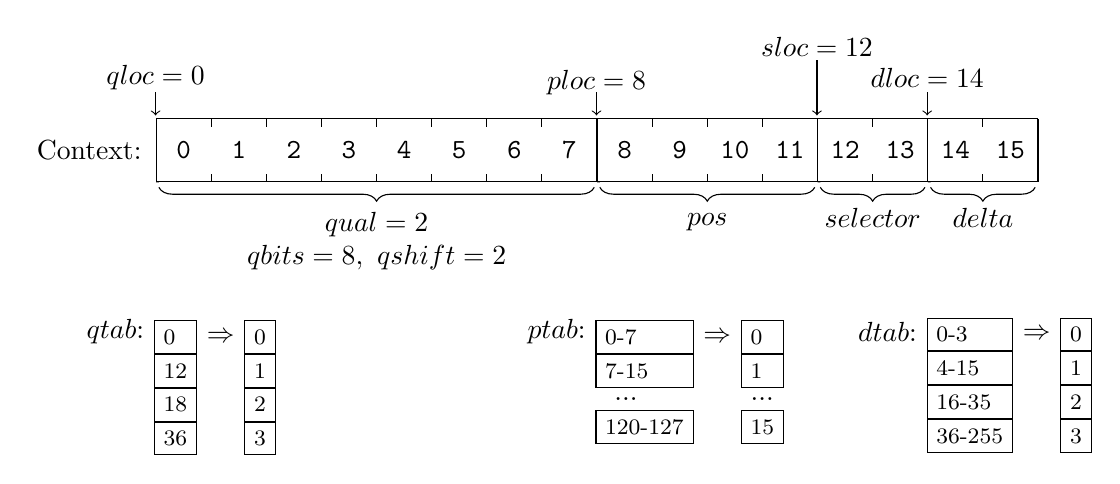
\begin{tikzpicture}[
  boxed/.style={rectangle, draw=black, text width=1cm},
  boxed1/.style={rectangle, draw=black},
  boxed2/.style={rectangle, draw=black, text width=.3cm},
  boxed3/.style={rectangle, draw=black, text width=0.85cm},
]
\newcommand{\x}{0.7cm}
\node at (-0.5, 0) {Context:};
\draw[-] (0*\x+.5*\x,-0.4) -- (0*\x+.5*\x,+0.4);
\foreach \w/\i [count=\n] in {
  3/0, 3/1, 3/2, 3/3, 3/4, 3/5, 3/6, 0/7,   % qual
  3/8, 3/9, 3/10, 0/11,                     % pos
  3/12, 0/13,                               % selector
  3/14, 0/15} {                             % delta
    \draw[-] (\n*\x+.5*\x,-0.4)  -- (\n*\x+.5*\x,-\w/10);
    \draw[-] (\n*\x+.5*\x,\w/10) -- (\n*\x+.5*\x, 0.4);
    \draw[-] (\n*\x-.5*\x,-0.4)  -- (\n*\x+.5*\x,-0.4);
    \draw[-] (\n*\x-.5*\x, 0.4)  -- (\n*\x+.5*\x, 0.4);
    \node(N\n)[minimum height=1cm,minimum width=\x,xshift=\n*\x,font=\ttfamily](N\n){\i};
}
\draw[<-] ([yshift=1pt]N1.north west)+(0,-0.1cm) -- +(0,0.2cm)
    node[yshift=5pt]{$qloc=0$};
\draw[<-] ([yshift=1pt]N9.north west)+(0,-0.1cm) -- +(0,0.2cm)
    node[yshift=3.5pt]{$ploc=8$};
\draw[<-] ([yshift=1pt]N13.north west)+(0,-0.1cm) -- +(0,0.6cm)
    node[yshift=5pt]{$sloc=12$};
\draw[<-] ([yshift=1pt]N15.north west)+(0,-0.1cm) -- +(0,0.2cm)
    node[yshift=5pt]{$dloc=14$};
\draw[decoration={brace,mirror,amplitude=5pt,raise=2pt, post=moveto, pre length=1pt, post length=1pt},decorate]
  (0.5*\x,-0.4) -- node[below=6pt] {\begin{tabular}{c}$qual \shiftl= 2$\\$qbits=8,\ qshift=2$\end{tabular}} +(8*\x,0);
\draw[decoration={brace,mirror,amplitude=5pt,raise=2pt, post=moveto, pre length=1pt, post length=1pt},decorate]
  (8.5*\x,-0.4) -- node[below=8pt] {$pos$} +(4*\x,0);
\draw[decoration={brace,mirror,amplitude=5pt,raise=2pt, post=moveto, pre length=1pt, post length=1pt},decorate]
  (12.5*\x,-0.4) -- node[below=6pt] {$selector$} +(2*\x,0);
\draw[decoration={brace,mirror,amplitude=5pt,raise=2pt, post=moveto, pre length=1pt, post length=1pt},decorate]
  (14.5*\x,-0.4) -- node[below=6pt] {$delta$} +(2*\x,0);

\node[right] (Q) at ([yshift=-1.8cm,xshift=-1cm]N1.south west) {$qtab$:};
\node[above right,boxed2] (Q0) at (Q.south east)  {\footnotesize{0}};
\node[below right,boxed2] (Q1) at (Q0.south west) {\footnotesize{12}};
\node[below right,boxed2] (Q2) at (Q1.south west) {\footnotesize{18}};
\node[below right,boxed2] (Q3) at (Q2.south west) {\footnotesize{36}};

\node[right] (Qeq) at (Q0.east) {$\Rightarrow$};
\node[      right,boxed1] (q0) at (Qeq.east) {\footnotesize{0}};
\node[below right,boxed1] (q1) at (q0.south west) {\footnotesize{1}};
\node[below right,boxed1] (q2) at (q1.south west) {\footnotesize{2}};
\node[below right,boxed1] (q3) at (q2.south west) {\footnotesize{3}};

%\node[right] (P) at ([xshift=3cm]Q.east) {$ptab$:};
\node[right] (P) at ([yshift=-1.8cm,xshift=-1cm]N9.south west) {$ptab$:};
\node[above right,boxed] (P0)   at (P.south east)  {\footnotesize{0-7}};
\node[below right,boxed] (P8)   at (P0.south west) {\footnotesize{7-15}};
\node[below right]       (P16)  at (P8.south west) {\ ...};
\node[below right,boxed] (P124) at (P16.south west) {\footnotesize{120-127}};

\node[right] (Peq) at (P0.east) {$\Rightarrow$};
\node[      right,boxed2] (p0)   at (Peq.east) {\footnotesize{0}};
\node[below right,boxed2] (p8)   at (p0.south west) {\footnotesize{1}};
\node[below right       ] (p16)  at (p8.south west) {...};
\node[below right,boxed2] (p124) at (p16.south west) {\footnotesize{15}};

%\node[right] (D) at ([xshift=4cm]P.east) {$dtab$:};
\node[right] (D) at ([yshift=-1.8cm,xshift=-1cm]N15.south west) {$dtab$:};
\node[above right,boxed3] (D0) at (D.south east)  {\footnotesize{0-3}};
\node[below right,boxed3] (D1) at (D0.south west) {\footnotesize{4-15}};
\node[below right,boxed3] (D2) at (D1.south west) {\footnotesize{16-35}};
\node[below right,boxed3] (D3) at (D2.south west) {\footnotesize{36-255}};

\node[right] (Ded) at (D0.east) {$\Rightarrow$};
\node[      right,boxed1] (d0) at (Ded.east) {\footnotesize{0}};
\node[below right,boxed1] (d1) at (d0.south west) {\footnotesize{1}};
\node[below right,boxed1] (d2) at (d1.south west) {\footnotesize{2}};
\node[below right,boxed1] (d3) at (d2.south west) {\footnotesize{3}};

\end{tikzpicture}
\end{center}

The entropy encoder used is shared between all models, so the bit
streams are multiplexed together.

The 16-bit quality value context is constructed by adding sub-contexts
together consisting of previous quality values, position along the
current record, a running count (per record) of how many times the
quality value has differed to the previous one (delta), and an
arbitrary stored selector value, each shifted to a defined location
within the combined context value ($qloc$, $ploc$, $dloc$ and
$sloc$ respectively).  The qual, pos and delta sub-contexts are
computed from the previous data while the selector, if used, is read
directly from the compressed data stream.  The selector may be used to
switch parameter sets, or simply to group quality strings into
arbitrary user-defined sub-sets.  The numeric values for each of these
components can be passed through lookup tables ($qtab$ for quality,
$ptab$ for positions, $dtab$ for running delta and $stab$ for turning
the selector $s$ into a parameter index $x$).  These all convert the
monotonically increasing range 0$\rightarrow$M to a (usually smaller)
monotonically increasing 0$\rightarrow$N.  For example if we wish to
use the approximate position along a 100 byte string, we may uniformly
map 0$\rightarrow$127 to 0$\rightarrow$15 to utilise 4 bits of our
16-bit combined context.

As some sequencing instruments produce binned qualities, e.g. 0, 10, 25,
35, these values are squashed to incremental values from 0 to
$max\_sym-1$ where $max\_sym$ is the maximum number of distinct
quality values observed.  If this transform is required, the flag
$have\_qmap$ will be set and a mapping table ($qmap$) will hold the
original quality values.  The decoded qualities will be the smaller
mapped range.

The quality sub-context is constructed by shifting left the previous
quality sub-context by $qshift$ bits and adding the current quality
after passing through the $qmap$ squashing process and if defined
through the $qtab$ lookup table.  The quality context is limited to
$qbits$ long and is added to the combined context starting at bit
$qloc$.  The quality sub-context is reset to zero at the start of each
new record.
\footnote{For example if we have 4 quality values in use -- 0, 10, 25 and
35 -- we will be encoding quality values 0, 1, 2 and 3.  We may wish to
define $qbits$ to be 6 and $qshift$ to be 2 such that the previous 3
quality values can be used as context, for the prediction of the next
quality value.  There will likely be little reason to use $qtab$ in
this scenario, but an encoder could define $qtab$ to convert \{0, 1, 2, 3\}
to \{0, 0, 0, 1\} and use $qshift$ of 1 instead, giving us
knowledge of which of the previous 6 values were maximum quality.}

The position context is simply the number of remaining quality values
in this record, so is a value starting at record length (minus 1) and
decrementing.  As with the quality context it may be passed through a
lookup table $ptab$ before shifting left by $ploc$ bits and adding to
the combined context.

Delta is a count of the number of times the quality value has changed
from one value to a different one.  Thus a run of identical values
will not increase delta.  It gets reset to zero at the start of every
record.  It may be adjusted by the $dtab$ lookup table and is shifted
by $dloc$ before adding to the combined context.

The selector value may also be used as a sub-context, if the $do\_sel$
paramter is set.  The initial context value (reset per record) is
defined within each parameter set, providing a more general purpose
alternative to adding the selector value at a defined location
($sloc$) into the context.

Thus the full context can be updated after each decoded quality with
the following pseudocode.  Note for brevity this is assuming the
$pos$, $delta$, $prevq$, $qctx$ and $sel$ parameters referred are global and updateable.

\begin{algorithmic}[1]
\Function{FQZUpdateContext}{$params, q$}
  \State $ctx \gets params.context$ \Comment{Also the initial value}
  \State $qctx \gets (qctx \shiftl params.qshift) + qtab_q$
  \State $ctx   \gets ctx + ((qctx \bitand (2^{params.qbits}-1)) \shiftl params.qloc)$
  \If{$params.pflags \bitand 32$} \Comment{$have\_ptab$}
    \State $p \gets $\Call{Min}{$pos$, $1023$}
    \State $ctx \gets ctx + (ptab_p \shiftl params.ploc)$
  \EndIf
  \If{$params.pflags \bitand 64$} \Comment{$have\_dtab$}
    \State $d \gets $\Call{Min}{$delta$, $255$}
    \State $ctx \gets ctx + (dtab_d \shiftl params.dloc)$
    \If{$prevq \ne q$}
      \State $delta \gets delta+1$
    \EndIf
    \State $prevq \gets q$
  \EndIf
  \If{$params.pflags \bitand 8$} \Comment{$do\_sel$}
    \State $ctx \gets ctx + (sel \shiftl params.sloc)$
  \EndIf
  \State \Return $ctx\bitand (2^{16}-1)$
\EndFunction
\end{algorithmic}

In summary context is produced using the following models:

\begin{table}[h]
\centering
\begin{tabular}{lrlp{9cm}}
 Model & Max symbol & Context size & Description\\
\hline
$model\_qual$ & $max\_sym$ & $2^{16}$ & Primary model for quality values \\
$model\_len$  & 256        & 4       & Read length models with the context 0-3 being successive byte numbers (little endian order) \\
$model\_rev$  & 2          & none    & Used if $pflags.do\_rev$ is defined.  Indicating which strings to reverse. \\
$model\_dup$  & 2          & none    & Used if $pflags.do\_dup$ is defined.  Indicates if this whole string is a duplicate of the last one \\
$model\_sel$  & $max\_sel$ & none    & Used if $gflags.multi\_param$ or $pflags.do\_sel$ are defined. \\
\end{tabular}
\end{table}

\pagebreak
\subsection{FQZComp Data Stream}

The start of an FQZComp data stream consists of the parameters used by
the decoder. The data layout is as follows.

\begin{table}
\centering
\begin{tabular}{|r|r|r|r|r|p{8cm}|l|l|}
\hline
\multicolumn{3}{|r|}{\textbf{Bits} }                   & \textbf{Type}  & \textbf{Name}                  & \multicolumn{3}{p{8.8cm}|}{\textbf{Description}} \\
\hline
\multicolumn{3}{|r|}{8}                                & uint8          & $version$                      & \multicolumn{3}{p{8.8cm}|}{FQZComp format version: must be 5}\\
\hline
\multicolumn{3}{|r|}{8}                                & uint8          & $gflags$                       & \multicolumn{3}{p{8.8cm}|}{Global FQZcomp bit-flags. From lowest bit to highest:}\\
\multicolumn{3}{|r|}{}                                 &                &                                & \multicolumn{3}{p{8.8cm}|}{1: $multi\_param$: indicates more than one parameter block is present.  Otherwise set $nparam = 1$} \\
\multicolumn{3}{|r|}{}                                 &                &                                & \multicolumn{3}{p{8.8cm}|}{2: $have\_stab$: indicates the parameter selector is mapped through $stab$.  Otherwise set $stab_i = i$} \\
\multicolumn{3}{|r|}{}                                 &                &                                & \multicolumn{3}{p{8.8cm}|}{4: $do\_rev$: $model\_revcomp$ will be used. (CRAM v3.1)} \\
\hline

\multicolumn{8}{|l|}{}\\[-0.7em]
\multicolumn{8}{|l|}{\textit{If $multi\_param$ gflag is set:} } \\
\cline{2-7}
                       & \multicolumn{2}{r|}{8}        & uint8          & \multicolumn{1}{r|}{$nparam$ } & \multicolumn{2}{p{8.4cm}|}{Number of parameter blocks (defaults to 1)} & \\
\cline{2-7}

\multicolumn{8}{|l|}{}\\[-0.5em]
\multicolumn{8}{|l|}{\textit{If $have\_stab$ gflag is set:} }                                                                                                                                 \\
\cline{2-7}
                       & \multicolumn{2}{r|}{8}        & uint8          & $max\_sel$                     & \multicolumn{2}{p{8.4cm}|}{Maximum parameter selector value} & \\
                       & \multicolumn{2}{r|}{variable} & table          & $stab$                         & \multicolumn{2}{p{8.4cm}|}{Parameter selector table} & \\
\cline{2-7}
\multicolumn{8}{|l|}{}\\
\hline
\hline
\multicolumn{8}{|l|}{}\\[-0.7em]
\multicolumn{8}{|l|}{\textit{Parameter block: repeated $nparam$ times: (selected via $model\_sel$ and $stab$)}} \\
\cline{2-7}
                       & \multicolumn{2}{r|}{16}        & uint16        & $context$                      & \multicolumn{2}{p{8.4cm}|}{Starting context value} & \\
\cline{2-7}
                       & \multicolumn{2}{r|}{8}        & uint8          & $pflags$                       & \multicolumn{2}{p{8.4cm}|}{Per-parameter block bit-flags. From lowest bit to highest:} & \\
                       & \multicolumn{2}{r|}{}         &                &                                & \multicolumn{2}{p{8.4cm}|}{1: Reserved} & \\
                       & \multicolumn{2}{r|}{}         &                &                                & \multicolumn{2}{p{8.4cm}|}{2: $do\_dedup$: model\_dup will be used} & \\
                       & \multicolumn{2}{r|}{}         &                &                                & \multicolumn{2}{p{8.4cm}|}{4: $do\_len$: model\_len will be used for every record.} & \\
                       & \multicolumn{2}{r|}{}         &                &                                & \multicolumn{2}{p{8.4cm}|}{8: $do\_sel$: model\_sel will be used.} & \\
                       & \multicolumn{2}{r|}{}         &                &                                & \multicolumn{2}{p{8.4cm}|}{16: $have\_qmap$: indicates quality map is present} & \\
                       & \multicolumn{2}{r|}{}         &                &                                & \multicolumn{2}{p{8.4cm}|}{32: $have\_ptab$: Load $ptab$, otherwise position contexts are unused} & \\
                       & \multicolumn{2}{r|}{}         &                &                                & \multicolumn{2}{p{8.4cm}|}{64: $have\_dtab$: Load $dtab$, otherwise delta contexts are unused} & \\
                       & \multicolumn{2}{r|}{}         &                &                                & \multicolumn{2}{p{8.4cm}|}{128: $have\_qtab$: Load $qtab$, otherwise set $qtab_i = i$} &\\
\cline{2-7}
                       & \multicolumn{2}{r|}{8}        & uint8          & $max\_sym$                     & \multicolumn{2}{p{8.4cm}|}{Total number of distinct quality values} & \\
\cline{2-7}
                       & \multicolumn{2}{r|}{4}        & uint4 (high)   & $qbits$                        & \multicolumn{2}{p{8.4cm}|}{Total number of bits for quality context} & \\
                       & \multicolumn{2}{r|}{4}        & uint4 (low)    & $qshift$                       & \multicolumn{2}{p{8.4cm}|}{Left bit shift per successive quality in quality context} & \\
                       & \multicolumn{2}{r|}{4}        & uint4 (high)   & $qloc$                         & \multicolumn{2}{p{8.4cm}|}{Bit position of quality context} & \\
                       & \multicolumn{2}{r|}{4}        & uint4 (low)    & $sloc$                         & \multicolumn{2}{p{8.4cm}|}{Bit position of selector context} & \\
                       & \multicolumn{2}{r|}{4}        & uint4 (high)   & $ploc$                         & \multicolumn{2}{p{8.4cm}|}{Bit position of position context} & \\
                       & \multicolumn{2}{r|}{4}        & uint4 (low)    & $dloc$                         & \multicolumn{2}{p{8.4cm}|}{Bit position of delta context }& \\
\cline{2-7}

& \multicolumn{6}{l|}{} & \\[-0.7em]
\multicolumn{1}{|l|}{} & \multicolumn{6}{l|}{ \textit{If $have\_map$ pflag is set:} } & \\
\cline{3-6}
                       &  & variable                   & uint8[$max\_sym$]          & $qmap$             & Map for unbinning quality values. & & \\
\cline{3-6}

& \multicolumn{6}{l|}{} & \\[-0.5em]
\multicolumn{1}{|l|}{} & \multicolumn{6}{l|}{ \textit{If $have\_qtab$ pflag is set:} } & \\
\cline{3-6}
                       &  & variable                   & table          & $qtab$                         & Quality context lookup table & & \\
\cline{3-6}

& \multicolumn{6}{l|}{} & \\[-0.5em]
\multicolumn{1}{|l|}{} & \multicolumn{6}{l|}{ \textit{If $have\_tab$ pflag is set:} } & \\
\cline{3-6}
                       &  & variable                   & table          & $ptab$                         & Position context lookup table & & \\
\cline{3-6}

& \multicolumn{6}{l|}{} & \\[-0.5em]
\multicolumn{1}{|l|}{} & \multicolumn{6}{l|}{ \textit{If $have\_tab$ pflag is set:} } & \\
\cline{3-6}
                       &  & variable                   & table          & $dtab$                         & Delta context lookup table & & \\
\cline{3-6}
& \multicolumn{6}{l|}{} & \\
\cline{2-7}
\multicolumn{8}{|l|}{}\\
\hline
\end{tabular}
\end{table}

% As an example configuration, with 8 distinct quality values we would
% use $qmap$ to encode/decode qualities in the range 0-7 and can do
% Order-3 entropy encoding by setting $qbits=9$ and $qshift=3$.  This
% leaves 7 bits remaining, which would could distribute as 3 bits of
% position (perhaps pos/16 or pos/32 to get approximate location), 3
% bits of running delta/4, and a bit to distinguish READ1 from READ2.
% Disagramatically the combined context layout would look this this:
%
% \includegraphics[width=250pt, keepaspectratio=true]{img/fqz_bits.png}
% FIXME: read2 becomes selector?
%
% In parameter terms we would use these values in the parameter block:
%
% \begin{tabular}{lrl}
% \hline
% \textbf{Field} & \textbf{Value} & \textbf{Note}\\
% \hline
% qbits  & 9  & 3 bit each $\implies$ Order-3 Markov model \\
% qshift & 3  & E.g. HiSeq X 8-binned, as 3 bit qmap \\
% qloc   & 0  & No $qtab$ needed, but $qmap$ converts qual to 0-7 range.\\
% \hline
% ploc   & 9  & With $ptab$ performing pos/32 function.\\
% \hline
% dloc   & 12 & With $dtab$ performing delta/4 function.\\
% \hline
% rloc   & 15 & 1 bit, iff $do\_read2$ flag is set\\
% \hline
% \end{tabular}
%
% FIXME: our worked example should include actual bytes for qmap, ptab
% and dtab too.


\textsc{FQZDecodeParams} below describes the pseudocode for reading
the parameter block.

\begin{algorithmic}[1]
\Procedure{FQZDecodeParams}{}
  \State $vers \gets $\Call{ReadUint8}{}
  \If{$vers \ne 5$}
    \State ERROR
  \EndIf
  \State $gflags \gets$ \Call{ReadUint8}{}
  \If{$gflags \bitand 1$} \Comment{$multi\_param$}
    \State $nparam \gets$ \Call{ReadUint8}{}
    \State $max\_sel \gets nparam$
  \Else
    \State $nparam \gets 1$
    \State $max\_sel \gets 0$
  \EndIf
  \If{$gflags \bitand 2$} \Comment{$have\_stab$}
    \State $max\_sel \gets$ \Call{ReadUint8}{}
    \State $stab \gets$ \Call{ReadArray}{$256$}
  \EndIf
  \State $max\_sym \gets 0$
  \For{$p \gets 0$ to $nparam-1$}
    \State $param_p \gets$ \Call{FQZDecodeSingleParam}{}
    \If {$max\_sym < param_p.max\_sym$}
      \State $max\_sym \gets param_p.max\_sym$ \Comment{Maximum across all param sets}
    \EndIf
  \EndFor
\EndProcedure
\end{algorithmic}

\begin{algorithmic}[1]
\Function{FQZDecodeSingleParam}{}
  \settowidth{\maxwidth}{p.have\_qtab\ }
  \State \algalign{p.context}{\gets} \Call{ReadUint16}{}
  \State \algalign{p.flags}{\gets} \Call{ReadUint8}{}
%  \State \algalign{have\_qtab}{\gets}    $p.flags\bitand 128$
%  \State \algalign{have\_dtab}{\gets}    $p.flags\bitand 64$
%  \State \algalign{have\_ptab}{\gets}    $p.flags\bitand 16$
%  \State \algalign{do\_rev}{\gets}    $flags\bitand 16$
%  \State \algalign{do\_sel}{\gets} $flags\bitand 8$
%  \State \algalign{do\_len}{\gets}    $flags\bitand 4$
%  \State \algalign{do\_dedup}{\gets}  $flags\bitand 2$
%  \State \algalign{have\_qmap}{\gets}   $flags\bitand 1$
  \State \algalign{p.max\_sym}{\gets} \Call{ReadUint8}{}
  \State \algalign{p.first\_len}{\gets} $1$

  \settowidth{\maxwidth}{p.qshift\ }
  \State \algalign{x}{\gets} \Call{ReadUint8}{}
  \State \algalign{p.qbits}{\gets} $x \bdiv 16$
  \State \algalign{p.qshift}{\gets} $x \bmod 16$
  \State \algalign{x}{\gets} \Call{ReadUint8}{}
  \State \algalign{p.qloc}{\gets} $x \bdiv 16$
  \State \algalign{p.sloc}{\gets} $x \bmod 16$
  \State \algalign{x}{\gets} \Call{ReadUint8}{}
  \State \algalign{p.ploc}{\gets} $x \bdiv 16$
  \State \algalign{p.dloc}{\gets} $x \bmod 16$

  \If{$p.flags\bitand 1$} \Comment{Have qmap}
    \For{$i \gets 0$ to $p.max\_sym-1$}
      \State $p.qmap_i \gets$ \Call{ReadUint8}{}
    \EndFor
  \EndIf

  \If{$p.flags\bitand 128$} \Comment{Have qtab}
    \State $p.qtab \gets$ \Call{ReadArray}{$256$}
  \Else
    \For{$i \gets 0$ to $256$}
      \State $p.qtab_i \gets i$
    \EndFor
  \EndIf

  \If{$p.flags\bitand 16$} \Comment{Have ptab}
    \State $p.ptab \gets$ \Call{ReadArray}{$1024$}
  \EndIf

  \If{$p.flags\bitand 64$} \Comment{Have dtab}
    \State $p.qtab \gets$ \Call{ReadArray}{$256$}
  \EndIf

  \State \Return $p$
\EndFunction
\end{algorithmic}

\textsc{FQZCreateModels} creates the decoder models based on the above
parameters and the shared range coder.

\begin{program}[H]
\begin{algorithmic}[1]
\Procedure{FQZCreateModels}{}
  \State $rc \gets $\Call{RangeDecodeCreate}{}
  \For{$i \gets 0$ to $3$}
    \State $model\_len_i \gets $\Call{ModelCreate}{$256$}
  \EndFor
  \For{$i \gets 0$ to $2^{16}-1$}
    \State $model\_qual_i \gets $\Call{ModelCreate}{$max\_sym+1$}
  \EndFor
  \State $model\_dup \gets $\Call{ModelCreate}{$2$}
  \State $model\_rev \gets $\Call{ModelCreate}{$2$}
  \If{$max\_sel > 0$}
    \State $model\_sel \gets $\Call{ModelCreate}{$max\_sel+1$}
  \EndIf
\EndProcedure
\end{algorithmic}
\end{program}

\textsc{ReadArray} reads an array $A$ of size $n$ which maps values 0
to $n-1$ to a smaller range (0 to $m-1$), both monotonically
increasing.  For efficiency this is done using a two-level run length
encoding.

Assuming $m < n$ there will be runs of the same value.  We measure run
lengths for all values (even if they are zero).  For example an array
$A = \{0,1,3,4,5,6,7,7,7,7\}$ may be converted to run lengths $R =
\{1,1,0,1,1,1,1,4\}$.  To keep values in this array fitting within one
byte, long runs are broken down in a successive series of 255 values,
so a run of length 600 becomes 255 255 90.

This array $R$ is no longer monotonically increasing but may still
have repeated values, so is run-length encoded by storing the number
of additional values whenever the last two lengths match.  This
converts $R$ to $R2 = \{1, 1, +0, 0, 1, 1, +2, 4\}$ where the `+'
symbol is shown purely to indicate the values representing the
additional run-length copy numbers.  (This also now turns the example
run of 600 above into 255 255 0 90.)

The final array $R2$ is the stored data stream.  The decoder process
is the reverse of the above, starting by converting $R2$ to $R$ and
then $A$.  The following pseudocode demonstrates this process.

\begin{algorithmic}[1]
\Function{ReadArray}{n}
\State $i,j,z \gets 0$
\State $last \gets -1$
\While{$z < n$} \Comment{Convert $R2$ to $R$}
  \State $run \gets $ \Call{ReadUint8}{}
  \State $R_j \gets run$
  \State $j \gets j+1$
  \State $z \gets z + run$
  \If{$run = last$}
    \State $copy \gets $ \Call{ReadUint8}{}
    \For{$x \gets 1 $ to $copy$}
      \State $R_j \gets run$
      \State $j \gets j+1$
    \EndFor
    \State $z \gets z + run \times copy$
  \EndIf
  \State $last \gets run$
\EndWhile
\Statex
\State $i,j,z \gets 0$
\While{$z < n$} \Comment{Convert $R$ to $A$}
  \State $run\_len \gets 0$
  \Repeat
    \State $part \gets R_j$
    \State $j \gets j + 1$
    \State $run\_len \gets run\_len + part$
  \Until{$part \ne 255$}
  \For{$x \gets 1 $ to $run\_len$}
    \State $A_z \gets i$
    \State $z \gets z+1$
  \EndFor
  \State $i \gets i+1$
\EndWhile
\Statex
\State \Return $A$
\EndFunction
\end{algorithmic}

The main loop decodes data in the following order per read:  read
length (if not fixed), the flag for whether this is read 2 (if
needed), a bit flag to indicate if the quality is duplicated (if
needed), followed by record length number of quality values using
various data gathered since the start of this read as context.

The output of this function is an array of quality values in the
variable $output$, indexed with the $i^{th}$ value via $output_i$.
The output buffer is a concatenation of all quality values for each
record.  The record lengths are recorded, but note this is the number
of qualities encoded in CRAM for this sequence record and this does
not necessarily have to match the number of base calls (for example
where qualities are explicitly specified for SNP bases but not
elsewhere).

\algnewcommand{\algorithmicgoto}{\textbf{go to}}%
\algnewcommand{\Goto}[1]{\algorithmicgoto\ \texttt{#1}}%
\algnewcommand{\Label}{\State\unskip}

\begin{algorithmic}[1]
\Function{FQZNewRecord}{}
  \State $sel \gets 0$
  \State $x \gets 0$
  \If{$max\_sel > 0$} \Comment{Find parameter selector}
    \State $sel \gets model\_sel.$\Call{ModelDecode}{$rc$}
    \If{$have\_stab$}
       \State $x \gets stab_{sel}$
    \EndIf
  \EndIf
  \State $param \gets params_x$

  \Statex
  \If{$param.do\_len \logor param.first\_len$} \Comment{Decode read length}
    \State $rec\_len \gets $\Call{DecodeLength}{rc}
    \State $param.last\_len \gets rec\_len$
    \If{$param.do\_len = 0$}
      \State $param.first\_len = 0$
    \EndIf
  \Else
    \State $rec\_len \gets param.last\_len$
  \EndIf
  \State $pos \gets rec\_len$

  \Statex
  \If{$param.do\_rev$} \Comment{Check if needs reversal}
    \State $rev_{rec} \gets model\_rev.$\Call{ModelDecode}{$rc$}
    \State $len_{rec} \gets rec\_len$
  \EndIf
  \State $rec \gets rec+1$

  \Statex
  \State $is\_dup \gets 0$
  \If{$do\_dedup$} \Comment{Duplicate last string if appropriate}
    \If{$model\_dup.$\Call{ModelDecode}{$rc$} > 0}
      \State $is\_dup \gets 1$
    \EndIf
  \EndIf
  \Statex
  \State $qctx \gets 0$
  \State $delta \gets 0$
  \State $prevq \gets 0$
  \State \Return $x$\Comment{Tabulated parameter selector}
\EndFunction
\end{algorithmic}

\begin{algorithmic}[1]
\Procedure{FQZDecode}{}
  \State $buf\_len \gets$ \Call{ReadUint7}{}
  \State \Call{FQZDecodeParams}{}
  \State \Call{FQZCreateModels}{}
  \State $i \gets 0$\Comment{Position in total quality block}
  \State $pos \gets 0$\Comment{Remaining base count current quality string}
  \Label \texttt{next\_record:}
  \While{$i < buf\_len$}
    \If{$pos = 0$}\Comment{Reset state at start of each new record}
      \State $x \gets $\Call{FQZNewRecord}{}
      \If {$is\_dup = 1$}
        \For{$j \gets 0$ to $rec\_len-1$}
          \State $output_{i+j} \gets output_{i+j-rec\_len}$
        \EndFor
        \State $i \gets i+rec\_len$
        \State $pos \gets 0$
        \State \Goto{next\_record}
      \EndIf

      \Statex
      \State $param \gets params_x$
      \State $ctx \gets param.context$
    \EndIf
    \Statex
    \State $q \gets model\_qual_{ctx}.$\Call{ModelDecode}{$rc$}
    \Comment{Decode a single quality value}
    \If{$param.have\_qmap$}
      \State $output_i \gets qmap_q$
    \Else
      \State $output_i \gets q$
    \EndIf
    \Statex
    \State $ctx \gets $\Call{FQZUpdateContext}{$param, q$}\Comment{Also updates qlast, prevq and delta}
    \Statex
    \State $i \gets i + 1$
    \State $pos \gets pos - 1$
  \EndWhile
  \If{$do\_rev$}
    \State \Call{ReverseQualities}{$output,\ buf\_len,\ rev,\ len$}
  \EndIf
\EndProcedure
\end{algorithmic}

Read lengths are encoded as 4 8-bit bytes, each having its own model.

\begin{algorithmic}[1]
\Function{DecodeLength}{rc}
\State $rec\_len \gets model\_len_0.$\Call{ModelDecode}{$rc$}
\State $rec\_len \gets rec\_len + (model\_len_1.$\Call{ModelDecode}{$rc$}$ \shiftl 8)$
\State $rec\_len \gets rec\_len + (model\_len_2.$\Call{ModelDecode}{$rc$}$ \shiftl 16)$
\State $rec\_len \gets rec\_len + (model\_len_3.$\Call{ModelDecode}{$rc$}$ \shiftl 24)$
\State \Return $rec\_len$
\EndFunction
\end{algorithmic}

For CRAM v4.0 quality values are stored in their original FASTQ
orientation.  For CRAM v3.1 they are stored in their alignment
orientation and it may be beneficial for compression purposes to
reverse them first.  If so $do\_rev$ will be set and the
\textsc{ReverseQualities} procedure called below after decoding.

\begin{algorithmic}[1]
\Procedure{ReverseQualities}{$qual,\ qual\_len,\ rev,\ len$}
\State $rec \gets 0$
\State $i \gets 0$
\While{$i < qual\_len$}
  \If{$rev_{rec} \ne 0$}
    \State $j \gets 0$
    \State $k \gets len_{rec}-1$
    \While{$j < k$}
      \State \Call{Swap}{$qual_{i+j}$, $qual_{i+k}$}
      \State $j \gets j+1$
      \State $k \gets k-1$
    \EndWhile
    \State $i \gets i + len_{rec}$
    \State $rec \gets rec+1$
  \EndIf
\EndWhile
\EndProcedure
\end{algorithmic}




\end{document}
